%        File: main.tex
%     Created: Thu Oct 27 09:00 PM 2011 C
% Last Change: Thu Oct 27 09:00 PM 2011 C
%
\documentclass[a4paper,12pt]{book}
\usepackage[utf8]{inputenc}
\usepackage[francais]{babel}
\usepackage{graphicx}
\usepackage{amsmath}
%\usepackage{fullpage}
\usepackage{setspace}
\usepackage{mathrsfs} %lettre ronde

\setstretch{1.2}

\begin{document}
\author{Romain Vincent} 
\title{\Huge Détection d'un spin nucléaire unique à l'aide d'un transistor de spin} 
\date{Décembre 2012}
\maketitle
\thispagestyle{empty}

\frontmatter 
\sloppy %permet de forcer certains retours à la ligne plutôt qu'un mot qui dépasse
\tableofcontents
<<<<<<< HEAD
\part{Théorie}



\chapter{Transport mésoscopique}

Nous allons dans ce chapitre aborder quelques notions de transport mésoscopique essentielles à la compréhension des résultats présentés dans la suite de cette thèse. La physique mésoscopique traite des systèmes de petites tailles, habituellement de la dizaine ou de la centaine de nanomètres~(parfois moins). Le transport mésoscopique s'intéresse plus particulièrement à la façon dont les électrons vont pouvoir circuler mais aussi interagir dans de telles structures pour donner naissance à des phénomènes quantiques tels que l'éffet Kondo ou le blocage de Coulomb. 

Il s'agit d'un domaine bien trop riche pour être traité dans un chapitre introductif et je concentrerai donc mon propos sur trois phénomènes déjà largement étudiés. Deux de ces phénomènes ont un point commun historique en cela qu'ils ont été découverts et expliqués bien avant la naissance de la physique mésoscopique telle que nous la connaissons aujourd'hui.

Le blocage de Coulomb par exemple que nous aborderons dans la première partie a été pour la première fois mis en évidence en 1951 par C.J. Gorter. Il avait constaté qu'en mesurant la conductance d'un matériau métallique granuleux à basse température, celle-ci diminuait de façon inattendue. Il expliquait cette baisse de conductance par la répulsion coulombienne au sein des grains de métaux composant son matériaux. Nous montrerons comment ce phénomène joue un rôle central dans le transport à travers des structures mésoscopiques.

L'effet Kondo que nous introduirons en fin de chapitre a lui aussi été mis en évidence dans la première partie du siècle dernier~(dans les années 1930) par des mesures sur des échantillons de métaux massif contenant des impuretés magnétiques. Les mesures de conductances à basse température avait montré qu'après avoir atteint un maximum, la conductance diminuait à nouveau. L'explication du phénomène n'a pas été immédiate et ce n'est qu'en 1964 que Jung Kondo a pu fournir une explication satisfaisante. Selon lui, les impuretés magnétiques agissent, à basse température, comme des centres diffuseurs très actifs diminuant d'autant la conductance de l'échantillon. Je donnerai plus de détails sur ce phénomène dans la suite du chapitre. En particulier, je détaillerai comment l'effet Kondo se manifeste dans les systèmes mésoscopiques.

Nous aborderons également un autre phénomène, le cotunneling, qui permet aux électrons de s'affranchir pendant un temps très court du régime de blocage de Coulomb. Nous verrons que ceci n'est possible que de part les lois de la physique quantique. Pour cela, nous distinguerons deux situation, l'une dans lequel aucun apport en énergie n'est nécessaire au phénomène - le cotunneling élastique- et une seconde pour laquelle if faudra fournir un certaine énergie au système - le cotunneling inélastique.

Afin d'étudier ces différents phénomènes, nous commencerons par définir les paramètres de notre système. En particulier, nous détaillerons chacun des éléments qui le composent ainsi que l'influence des paramètres qui le caractérisent. Nous poursuivrons ensuite par la définition et l'illustration du concept de potentiel chimique dans le cadre du transport mésoscopique. Nous verrons comment cette notion permet de façon simple et intuitive de comprendre quelles sont les conditions pour qu'un courant traverse le système.

Quand cela sera possible, nous préciserons pour chacun de ces phénomènes les conditions nécessaires à leur observation ainsi que les variables expérimentales dont ils dépendent.
%%%%%%%%%%%%%%%%%%%%%%%%
%SECTION I
%%%%%%%%%%%%%%%%%%%%%%%%


\section{Les paramètres du système}
Dans le cadre de nos expériences, nous avons utilisé ce que l'on appelle un transistor à électron unique ou Single Electron Transistor~(SET). En général un tel système est composé d'un point quantique~(ou ilôt) connecté à trois terminaux que l'on nommera source, drain et grille~(en référence aux transistors à effet de champ). L'il\^ot est couplé à ces trois terminaux par trois capacitances : $C_g$ pour la grille, $C_d$ pour le drain et $C_s$ pour la source. De plus, des barrière tunnel entre le point quantique,la source et le drain permettent le passage d'électron (sous certaines conditions) et sont caractérisées par les paramètre $\gamma_s$~(source/il\^ot) et $\gamma_d$~(drain/il\^ot). La source et le drain sont considérés comme des matériaux métalliques massifs et dont les électrons obéissent à la statistique de Fermi-Dirac. Enfin, nous attribuons à l'il\^ot une taille caractéristique $L$. 

Ce système, les paramètres qui le caractérisent ainsi qu'un schéma électrique équivalent sont représentés dans la Fig. \ref{description_systeme}. Nous allons maintenant détailler chacun de ces éléments.


\subsection{Les capacitances du système}
Comme expliqué précédemment, trois capacitances couplent l'il\^ot central aux trois terminaux. L'application d'un tension sur l'un ou plusieurs de ces terminaux va donc modifier l'énergie du point quantique. Cette modification s'exprime comme suit :

\begin{eqnarray}
E = \frac{(C_sV_s + C_dV_d + C_gV_g)^2}{2(C_g + C_s + C_g)}=\frac{(C_sV_s + C_dV_d + C_gV_g)^2}{2C_{\Sigma}} \nonumber
\end{eqnarray}




Ces capacitances vont également induire un "co\^ut" énergétique à l'ajout d'un électron dans l'il\^ot central. Cet ajout est associé à l'énergie $E_c$ appelée énergie de charge dont la valeur est donnée par :
\begin{eqnarray}
\frac{E_c}{2} = \frac{e^2}{2(C_s+C_d+C_g)}=\frac{e^2}{2C_{\Sigma}} \nonumber
\end{eqnarray}


Cette énergie est à l'origine de la diminution de la conductance observée par C.J. Gorter en 1951. Lorsque la température est suffisamment élevée, elle fourni l'énergie nécessaire aux électrons pour passer d'un grain à l'autre. A basse température en revanche, les électrons n'ont plus la possibilité de se mouvoir de la sorte et la conductance mesurée diminue. On voit ici une première condition nécessaire à l'apparition du phénomène de blocage de Coulomb : $E_c \gg k_bT$.

En tenant compte de ces deux contributions, l'énergie d'un il\^ot contenant $N$ électrons et soumis à trois tensions $V_g$, $V_d$ et $V_s$ est donnée par :
\begin{eqnarray}
U(N) = \frac{1}{2C_{\Sigma}} (-|e|N + C_sV_s + C_dV_d + C_gV_g)^2
\end{eqnarray}

On inclus parfois dans cette expression une charge $eN_0$ pour tenir compte de l'environement électrostatique. Nous verrons en abordant la notion de potentiel chimique que seule la différence d'énergie entre les différents états de charge importe et que donc l'offset introduit par ce dernier terme peut \^etre ignoré. \newline

\fbox{\begin{minipage}{0.9\textwidth}
\textbf{Remarque :} dans les expériences de Microscopie à Effet Tunnel ou Scanning Tunneling Microscopie~(STM), seules les tensions de source et de drain peuvent \^etre modifiées. Ce désavantage est compensé par la possibilité de modifier les paramètres de couplage $\gamma$~(que l'on détaillera dans la suite) en modulant la distance séparant la pointe de l'échantillon.
\end{minipage}}

\begin{figure}
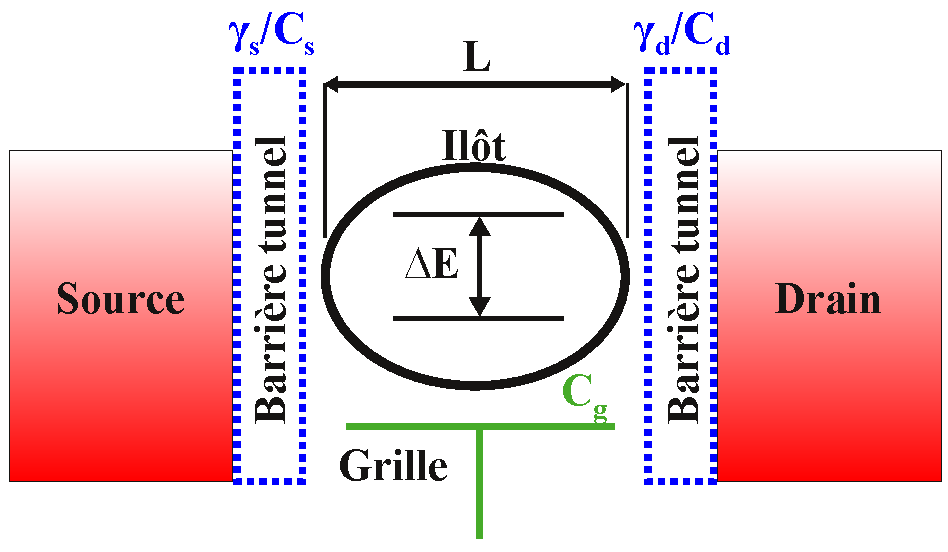
\includegraphics[scale=1]{Theorie/Transport/figure1/figure1ThTr.pdf} 
\caption{Paramètres caractérisant un système à trois terminaux}
\label{description_systeme}
\end{figure}



\subsection{L'il\^ot}
Les points quantiques que l'on utilise le plus fréquemment dans les expériences mésoscopiques sont souvent~(mais pas exclusivement) basés sur l'un des systèmes suivants:
\begin{itemize}
\item \textbf{un gaz d'électron bidimensionnel:} généralement une hétérostructre de semi-conducteur est utilisé pour obtenir un gaz d'électron bidimmensionnel proche de la surface. Par des technique de lithographie, des électrodes sont ajoutées sur l'échantillon. En appliquant une tension sur ces grilles, le gaz d'électron peut \^etre manipulé pour former un ou plusieurs points quantiques connectés à plusieurs électrodes.
\item \textbf{un grain métallique:} une grain de metal~(souvent noble) de quelques nanomètres joue le rôle de point quantique. Ces grains peuvent \^etre notamment obtenue en utilisant la technique d'électromigration que l'on verra dans la suite.
\item \textbf{une molécule:} c'est ce type de point quantique que nous utiliserons. Les molécule pouvant \^etre utilisées pour jouer ce r\^ole sont trop nombreuses pour toutes \^etre cité mais on donner quelques célèbres : les nanotubes, les fullerène, les aimants moléculaires etc.. \newline
\end{itemize}

Dans le cas d'électrons bidimensionnel ou celui d'un grain métallique, du fait de la taille des échantillons~($\sim 100nm$ pour les premiers, $\sim 10nm$ pour les seconds), on observe une quantification des différents états du système. Le spectre énergétique de l'il\^ot peut s'exprimer en fonction de trois nombres quantiques $n_x$, $n_y$ et $n_z$ à travers la relation suivante:
\begin{eqnarray}
E_n = \frac{\pi^2 \hbar^2}{2m}(\frac{n_x^2}{L_x^2} + \frac{n_y^2}{L_y^2} + \frac{n_z^2}{L_z^2}) \nonumber
\end{eqnarray}


Il s'agit bien entendu ici d'une expression très simplifiée car elle suppose une forme de potentiel de confinement difficile~(pour ne pas dire impossible) à obtenir en pratique (variation abrupte et hauteur de potentiel infini). Elle a le mérite en revanche de faire appara\^itre une deuxième condition nécessaire à l'observation de ce que l'on appelle habituellement le blocage de Coulomb quantique (par opposition au blocage de Coulomb classique où seul la quantification de la charge joue un rôle). En effet, pour résoudre le spectre de l'il\^ot, l'énergie associée à l'agitation thermique doit \^etre négligeable devant l'énergie séparant deux niveaux à savoir:

\begin{eqnarray}
\frac{\hbar^2}{2mL^2} \gg k_bT \nonumber
\end{eqnarray}

Si cette condition est facilement atteinte lorsque l'on utilise des gaz d'électrons bidimensionnels, elle est en revanche plus difficile à satisfaire dans le cas d'un point quantique métallique~(du fait d'une masse effective de l'électron très petite dans le premier cas contrairement au second). \newline


Lorsque des molécule sont utilisées, cette quantification apparait beaucoup plus naturellement à travers la notion d'orbitales moléculaires. En effet, c'est sur ces orbitales que vont venir s'ajouter les électrons lors de la charge de l'il\^ot. On désigne souvent la dernière orbitale contenant un électron par HOMO~(Highest Occupied Molecular Orbital). De même, la première orbitale ne contenant aucun électron est désignée par le terme LUMO~(Lowest Unoccupied Molecular Orbital).

Il faut se garder cependant de penser qu'une molécule jouant le r\^ole de point quantique conserve les m\^eme propriétés que cette m\^eme molécule isolée. Tout d'abord, les niveaux d'énergie sont fortement influencés par la présence des électrodes du fait de l'hybridisation. De plus, les électrodes peuvent induire une déformation qui va altérer la structure électronique de celle-ci. Ce phénomène est connu sour le nom d'effet Jhan-Teller. 

Nous montrerons par la suite que dans le cadre de l'électronique moléculaire et plus particulièrement celui de la spintronique moléculaire, il est important de pouvoir évaluer l'influence de ces différents phénomènes.

\subsection{Les paramètre de couplage tunnel $\gamma_{s/d}$}
On peut voir ces coefficient comme définissant "l'aisance" avec laquelle les électrons peuvent passer par effect tunnel de la source ou du drain vers l'il\^ot et vice-versas. Les valeurs $\gamma_{s/d}$ sont déterminantes dans la valeur du courant qui va \^etre mesuré dans notre système. Plus précisément, de leurs valeurs va dépendre la conductance $G$ de l'échantillon. Partant de cette conductance, on peut par un raisonnement simple montrer que celle-ci doit satisfaire la relation suivante:
\begin{eqnarray}
G \ll G_0 \text{ avec } G_0 = \frac{2e^2}{h}
\end{eqnarray}
où $G$ est la conductance de l'échantillon, $G_0$ est le quantum de conductance ($\sim 77.5 \mu S$), $e$ est la charge de l'électron et $h$ la constante de Planck.


De plus, le paramètre $\gamma$ rend compte de l'hybridisation des niveaux d'énergie du point quantique avec ceux des électrodes. Cette hybridisation entraîne l'élargissement des niveaux d'énergie d'une largeur $\Delta E_{\text{intrinsèque}}$ donnée par :
\begin{eqnarray}
\Delta E_{\text{intrinsèque}} = h (\gamma_s + \gamma_d)
\end{eqnarray}

Cette élargissement est appelé élargissement intrinsèque par opposition à l'élargissement induit par la température. On peut deviner ici une seconde condition nécéssaire à l'apparition du phénomène de blocage de Coulomb à savoir $\Delta E_{\text{intrinsèque}} \ll E_c$. De plus, dans un régime de blocage fort on a $\Delta E_{\text{intrinsèque}} \ll k_bT$. Si cette dernière condition est remplie, on peut avoir accès aux distributions de Fermi-Dirac des électrodes et donc ,à la température du système.




\section{La notion de potentiel chimique}
La notion de potentiel chimique est à mes yeux une des notions les plus importantes afin de comprendre de manière simple et intuitive le phénomène de blocage de Coulomb. Un exemple de son utilisation dans la cadre du transport quantique peut \^etre trouvé dans la très belle et très pédagogique revue de Hanson \textit{et Al.}. Dans cette section, nous allons tout d'abord présenter le concept de potentiel chimique. Nous exprimerons ensuite, à partir des considérations exposés dans la partie précédente, le potentiel chimique de la source, du drain et surtout de l'ilôt central.

\subsection{Définition}

On recontre souvent le potentiel chimique en thermodynamique lorsque l'on s'intéresse aux systèmes ouverts échangeant des particules~(cf. ensemble Grand Canonique). Cette grandeur défini la variation d'énergie d'un système d\^u à la modification du nombre de particules qui le compose. On le trouve parfois défini comme suit :
\begin{eqnarray}
\mu = \frac{\partial U}{\partial N} \nonumber
\end{eqnarray}
$U$ étant l'énergie du système et $N$ le nombre de particules. Dans la suite, nous allons plut\^ot adopter la notation de Hanson et Al. et prendre la définition suivante :
\begin{eqnarray}
\mu(N) = U(N) - U(N-1)
\end{eqnarray}
où $\mu(N)$ est le potentiel chimique de l'état de charge $N$, $U(N)$ et $U(N-1)$ étant respectivement l'énergie du système avec $N$ et $N-1$ particules.

\subsection{Expérience de pensé}

Partant de cette définition on peut imaginer un système de deux réservoirs contenant un grand nombre de particules, chacune d'entre elles possédant un potentiel chimique différent. Connectons les par un canal ne laissant passer qu'une particule de potentiel chimique $\mu_{canal}$. Si une particule du réservoir de droite possède ce potentiel chimique, elle peut donc passer dans le réservoir de gauche. Pour cela, elle passe tout d'abord du réservoir de droite au canal ce qui n'entra\^ine pas de variation dans l'énergie du système~($\Delta E = -\mu_{canal} + \mu_{canal} = 0$). De m\^eme, la particule peut ensuite passer du canal au réservoir de gauche. Les trois configurations : particule dans le réservoir de droite, de gauche ou dans le canal sont dégénérés et la particule peut circuler librement dans le système.

Supposons maintenant que le nombre de particules au potentiel chimique $\mu_{canal}$ soit plus grand dans le réservoir de droite que dans le réservoir de gauche. M\^eme si les particules de gauche peuvent circuler en direction du réservoir de droite, il y aura en proportion, plus de particules venant du réservoir de droite et allant vers le réservoir de gauche. Il y a donc un flux moyen de particules de la droite vers la gauche. Au bout d'un temps plus ou moins long, le système devrait tendre vers un équilibre et le flux vers zéro. En revanche, si l'on maintient "artificiellement" cette différence en nombre de particules, le flux devrait perdurer.

Dans le cadre de notre nanostructure, les particules sont des électrons, le nombre de particule au potentiel $\mu$ est gouverné par la distribution de Fermi pondéré par la densité d'état. Le canal filtrant n'est rien d'autre que notre point quantique. En introduisant un tension source drain, on induit une différence entre la source et le drain dans le nombre d'électron possédant le potentiel chimique $\mu$ tel que $\mu_s < \mu < \mu_d$~(cf Fig.\ref{distrib_fermi}.a). Un courant peut donc \^etre mesuré si le potentiel chimique du point quantique se trouve dans cette fen\^etre.

Ce raisonnement certe un peu simpliste peut \^etre formalisé aisément dans le cadre de la méthode des équations pilotes. L'ensemble de la procédure à suivre est détaillé dans l'annexe?!.



\subsection{Les potentiels chimique de la source et du drain.}
L'expression du potentiel chimique de la source et du drain est directement donnée par $\mu_i = e V_i$ ou $i=source/drain$. Il s'agit en fait du niveau de Fermi des électrons dans la source et le drain (à ne pas confondre avec l'énergie de Fermi). La probabilité dans un métal de niveau de fermi $\mu_F$ de trouvé un électron de potentiel chimique $\mu$ est donnée par la distribution de fermi:
\begin{eqnarray}
p(\mu) = \frac{1}{1 + \exp{(\frac{\mu - \mu_F}{k_bT})}} \nonumber
\end{eqnarray}
où $\mu$ est le potentiel chimique de l'électron, $\mu_F$ celui du métal, $k_b$ est la constante de Boltzmann et $T$ est la température du système. On obtient donc en fonction des tensions source et drain:
\begin{eqnarray}
p_i(\mu) = \frac{1}{1 + \exp{(\frac{\mu - eV_i}{k_bT})}}
\end{eqnarray}
ou $i$=source/drain, $V_i$ est la tension appliquée et $e$ la charge de l'électron. Comme nous l'avons vu dans notre expérience de pensé, cette notion est essentielle dans la détermination du courant qui traverse notre structure.

\begin{figure}
\centering 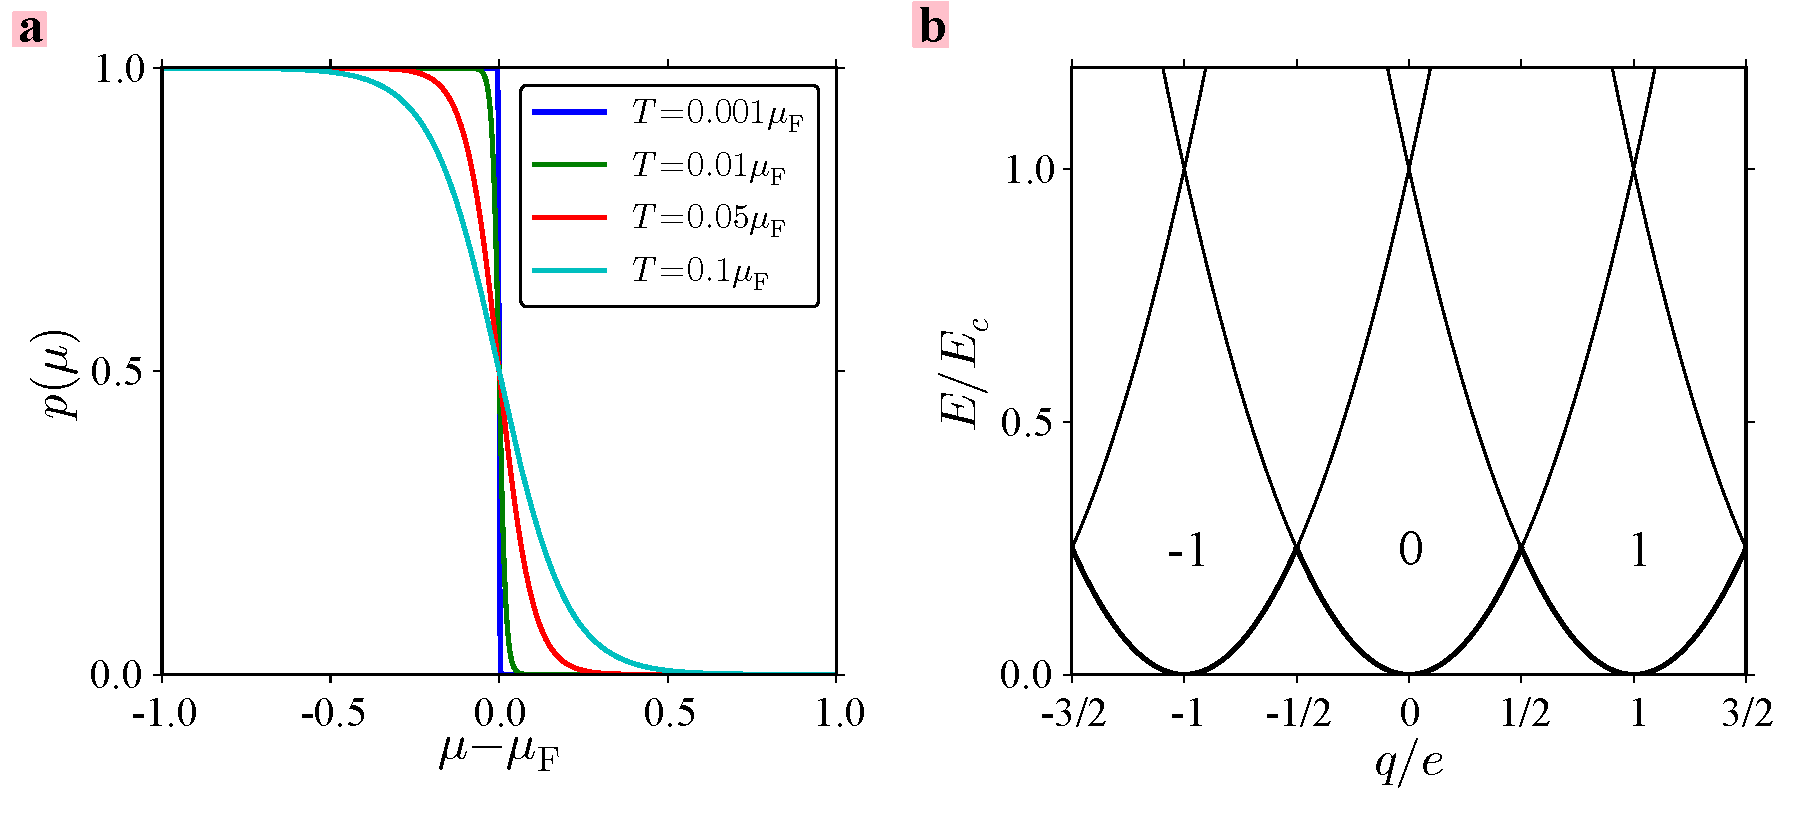
\includegraphics[scale=0.5]{Theorie/Transport/figure2/figure2.pdf} 
\caption{Probabilité d'avoir un électron de potentiel chimique $\mu$ sachant que le potentiel chimique du métal est $\mu_{\rm{F}}$. Le potentiel chimique $\mu_{\rm{F}}$ correspondant à une tension de $1mV$ que l'on applique habituellement dans ce genre d'éxpérience correspond à une énergie de $11.5K$.}
\label{distrib_fermi}
\end{figure}



\subsection{Le potentiel chimique de l'il\^ot}
Si l'expression du potentiel chimique de la source et du drain n'a rien de compliquée~(dans le cas d'électrode normale tout du moins), on ne peut pas en dire de m\^eme de celle de l'il\^ot. C'est m\^eme là que réside toute la difficulté de la compréhension d'une expérience. Heureusement, dans la partie précédente nous avons déjà fait le bilan des différentes énergie en jeux dans le système. A savoir, nous devons prendre en compte l'énergie électrostatique, l'énergie d'interaction électron-électron ainsi que la discrétisation des niveaux d'énergie dans l'il\^ot. Tout ceci donne :
\begin{eqnarray}
U(N) = \underbrace{\frac{1}{2C_{\Sigma}} (-|e|N + C_sV_s + C_dV_d + C_gV_g)^2}_{\text{couplage électrostatique et énergie de charge}}
+ 
\underbrace{\sum_{n=1}^{N} E_n}_{\substack{\text{énergie liés aux} \\\text{aux états discret}}}
\end{eqnarray}

On peut également tenir compte d'un éventuel champ magnétique en faisant le remplacement suivant :
\begin{eqnarray}
\sum_{n=1}^N E_n = \sum_{n=1}^N E_n(B) \nonumber
\end{eqnarray}
c'est à dire en attribuant à chaque niveau discret, une dépendance en champ magnétique. Nous verrons rapidement dans la suite comment cela se traduit dans le cas d'un système simple. 

Une fois l'énergie en fonction de $N$ exprimée simplement, il suffit d'appliquer la définition précédente à savoir :
\begin{eqnarray}
\mu(N) = U(N) - U(N-1) \nonumber
\end{eqnarray}

On se retrouve avec une expression relativement simple du potentiel chimique :
\begin{eqnarray}
\mu(N) = (N-\frac{1}{2})\frac{e^2}{C_{\Sigma}}
+ 
\frac{e}{C_{\Sigma}}(C_gV_g + C_sV_s + C_dV_d)
+
E_N(B)
\end{eqnarray}

En utilisant la définition de l'énergie de charge $E_c$ introduite précédemment, nous pouvons réécrire la relation sous la forme~(le terme 1/2 introduit précédemment permet une écriture plus compacte dans ce qui va suivre):

\begin{eqnarray}
\mu(N) = (N-\frac{1}{2})E_c
- 
\frac{E_c}{|e|}(C_gV_g + C_sV_s + C_dV_d)
+
E_N(B)
\label{pot_chim}
\end{eqnarray}

L'énergie $E_c$ est donc la quantité d'énergie d\^u à la répulsion Coulombienne qui sépare deux potentiels chimiques d'état de charge différents.


\section{Détermination des conditions de circulation d'un courant}
Pour rendre l'exposé qui va suivre plus clair, nous allons le décomposer en trois partie. Dans la première partie, nous allons voir quelles sont les conditions à remplir pour qu'un électron du drain puisse aller dans l'il\^ot. Dans la deuxième partie, nous ferrons de m\^eme pour la source. Enfin, dans la dernière partie, nous exploiterons les résultats obtenues pour en déduire les conditions nécessaires pour qu'un courant circule dans notre structure. Afin d'adapter les solutions trouvées aux conditions expérimentales, on posera $V_s = 0$ car dans la grande majorité des dispositifs, une des électrodes est directement connectée à la masse. Ce qui donnera $V_d=V_{ds}$, $V_{ds}$ étant la tension appliquée à l'échantillon.

\subsection{Charge de l'il\^ot par le drain}
Comme nous en avons discuté précédemment, pour qu'une particule (ici un électron) puisse passer d'un réservoir à l'autre, il faut que son potentiel chimique soit identique dans les deux réservoirs. Si l'on adapte se raisonnement à notre système, il faut donc qu'il y ait dans le drain des électrons dont le potentiel chimique corresponde à celui de cette électron une fois sur l'il\^ot. Supposons l'il\^ot dans l'état de charge $N-1$, pour passer à l'état de charge $N$, il faut qu'il y ait au moins un électron dans le drain dont le potentiel chimique soit égale à $\mu(N)$. Il nous suffit d'oberver la courbe de la Fig. \ref{distrib_fermi} pour comprendre que cela suppose :
\begin{eqnarray}
p(\mu) > 0 \Longrightarrow  -|e|V_{ds} \geq \mu(N) \nonumber
\end{eqnarray}

Ce qui conduit à la relation suivante :
\begin{eqnarray}
-|e|V_{ds} \geq (N-\frac{1}{2})\frac{e^2}{C_{\Sigma}}
-
\frac{|e|}{C_{\Sigma}}(C_gV_g + C_sV_s + C_dV_d)
+
E_N(B) \nonumber
\end{eqnarray}

En tenant compte des conditions $V_s= 0$ et que $V_{ds} = V_d$ évoquées plus haut, cette relation peut se réécrire de la façon suivante :
\begin{eqnarray}
V_{ds} \leq \frac{1}{C_g + C_s} \left\lbrace C_gV_g - \frac{C_{\Sigma}}{|e|}\left(E_N(B) + (N-\frac{1}{2})E_c \right) \right\rbrace 
\end{eqnarray}

La zone de transition entre charge et décharge dans le plan ($V_g$,$V_{ds}$) est délimité par une droite dont la pente $\dfrac{C_g}{C_g + C_s}$ determinée par les différentes capacitances du système.


\begin{figure}
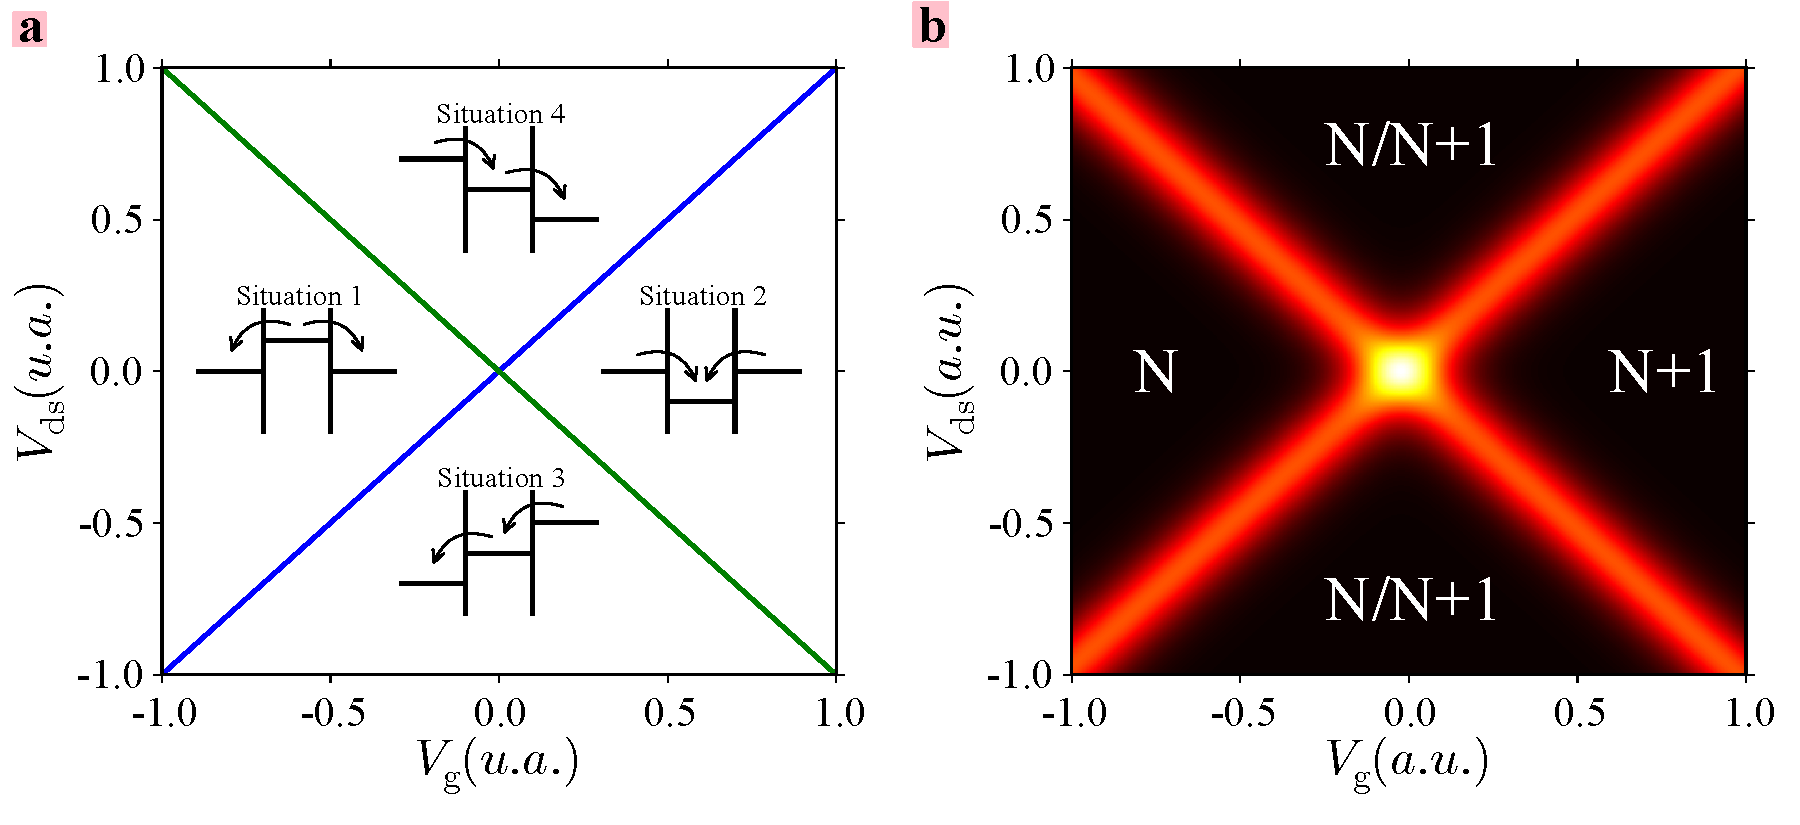
\includegraphics[scale=0.5]{Theorie/Transport/figure3/figure3.pdf} 
\caption{Représentation de la charge et de la décharge de l'il\^ot dans le plan ($V_g$,$V_{ds}$)}
\label{charge_discharge}
\end{figure}



\subsection{Charge de l'il\^ot par la source}
Un raisonnement similaire au précédent conduit à la relation suivante :

\begin{eqnarray}
V_{ds} \geq -\frac{1}{C_d} \left\lbrace C_gV_g + \frac{C_{\Sigma}}{|e|}\left( E_N(B) + (N-\frac{1}{2})E_c \right) \right\rbrace
\end{eqnarray}


On peut extraire une deuxième pente $-\dfrac{C_g}{C_d}$ qui correspond à la charge ou la décharge de l'il\^ot par la source.

Nous pouvons également déduire de ce qui précède une deuxième relations importantes. Deux états de charge consécutifs sont séparés par une tension de grille $\Delta V_g$ que l'on peut relier aux paramètres du système par la formule suivante:
\begin{eqnarray}
\frac{C_g}{C_{\Sigma}} |e| \Delta V_g = E_c + \Delta E
\end{eqnarray}
où $\Delta E = E_N(B) - E_{N-1}(B)$ est l'écart entre deux niveaux d'énergie du spectre discret.
\subsection{Condition de circulation du courant}

Si l'on reprend les deux paragraphes précédents, on peut imaginer quatre situations :
\begin{itemize}
\item \textbf{Situation 1} : aucun électron ne peut \^etre chargé ni par la source ni par le drain. L'état de charge reste à N.
\item \textbf{Situation 2} : un électron peut \^etre chargé à la fois par la source et par le drain. L'état de charge est donc fixé à N+1.
\item \textbf{Situation 3} : un électron ne peut \^etre chargé que par la source. Dans ce cas, il finit par se décharger dans le drain
\item \textbf{Situation 4} : un électron ne peut \^etre chargé que par le drain. Dans ce cas, il finit par se décharger dans la source. \newline
\end{itemize}

Dans les situations un et deux, l'état de charge de l'il\^ot est bien défini et on se trouve dans le régime de blocage de Coulomb. Dans la situation 3 les électrons circulent de la source vers le drain. Un courant positif est donc mesuré. Dans la situation 4, les électrons circulent du drain vers la source. Un courant négatif est donc mesuré. L'emsemble de ces régimes est représenté dans la Fig. \ref{charge_discharge}.a. 

Souvent, les mesures ne se font non pas en courant mais en conductance différentielle $dI/dV$. Une simulation d'une telle mesure obtenue par la méthode des équations pilote est présenté dans la  Fig.\ref{charge_discharge}.b où les différentes zones décrites précédemment sont séparées par de grande variations dans la conductance différentielle mesurée.\newline


\fbox{\begin{minipage}{0.90\textwidth}
\textbf{Remarque :} dans le cas d'une tension source-drain nulle, la condition de circulation de courant impose $\mu(N)=0$ soit $U(N)=U(N-1)$. Les deux états de charge sont dégénérés et on parle alors de point de dégénérescence. Un représentation de l'énergie $U(N)$ pour différents états de charge est représenté dans la Fig.\ref{distrib_fermi}.b.
\end{minipage}}



\section{Etats excités et transport}

Dans de nombreux cas, une transition d'un état de charge à l'autre ne peut pas être associée à un unique potentiel chimique du fait de la présence d'états excités pour l'un ou les deux états de charges. Il faut donc prendre en compte toutes les transitions afin de déterminer correctement la signature transport. Pour illustrer ceci, nous allons pendre un exemple simple dans lequel une boite quantique oscille entre les états de charges $N=0/1$. Nous tiendrons de plus compte du spin de l'électron. 

Sans champ magnétique appliqué le potentiel chimique $\mu_{+}$ associé à la transition d'un état de charge $N=0$ à un état de charge $N=1$ avec un état de spin up~($0\rightarrow +$) possède la m\^eme énergie que le potentiel chimique  $\mu_{-}$ associé la transition de l'état de charge $N=0$ à l'état de charge $N=1$ avec un état de spin down~($0\rightarrow -$).


Si l'on applique un champ magnétique au système, la dégénérescence en d'énergie des deux états de spin est levée du fait de l'effet Zeeman (cf Fig. \ref{charge_discharge}.b). Les deux potentiels chimiques $\mu_{-}$ et $\mu_{+}$ ne sont plus égaux. Le premier correspond désormais à la transition entre deux état fondamentaux~($EF(0)\rightarrow EF(1)$). Le second en revanche correspond à la transition de l'état fondamental de $N=0$ à l'état excité de $N=1$~($EF(0)\rightarrow EE(1)$).

On peut donc construire deux jeux de diamants de Coulomb, l'un correspondant à $\mu_{-}$ et l'autre à $\mu_{+}$~(cf Fig. \ref{charge_discharge}.a en bleu et rouge respectivement). Cependant, dans les zones de blocage associé au diamant de la transition $EF(0)\rightarrow EF(1)$ (représenté ici par le potentiel chimique $\mu_{-}$) , aucun courant de peut circuler (zone grisé dans la Fig.\ref{charge_discharge}.a). Les bords de diamant situés dans cette zone doivent apparaître en pointillés car ils ne correspondent pas réellement à une modification du courant.

De part cette construction, on constate que l'intersection entre les bord de diamant de la transistion $EF(0)\rightarrow EE(1)$ et ceux de la transition $EF(0)\rightarrow EF(1)$ donne une lecture directe de l'effet Zeeman (cf Fig. \ref{charge_discharge}.a). On peut donc par une mesure transport faire la spectroscopie du point quantique en fonction du champe magnétique. Dans ce cas prècis, celle-ci est fort simple.

 Cependant, dans la plus part des cas, les états N/N+1 possèdent tout deux des états fondamentaux et des états excités et l'analyse de la signature du système en transport devient plus difficile. Ces différentes configurations sont notamment traité par Hanson et Al., et un exemple peut \^etre trouvé dans l'analyse du $N@C_{60}$ et les références qu'elle contient proposée en fin de thèse.

\begin{figure}
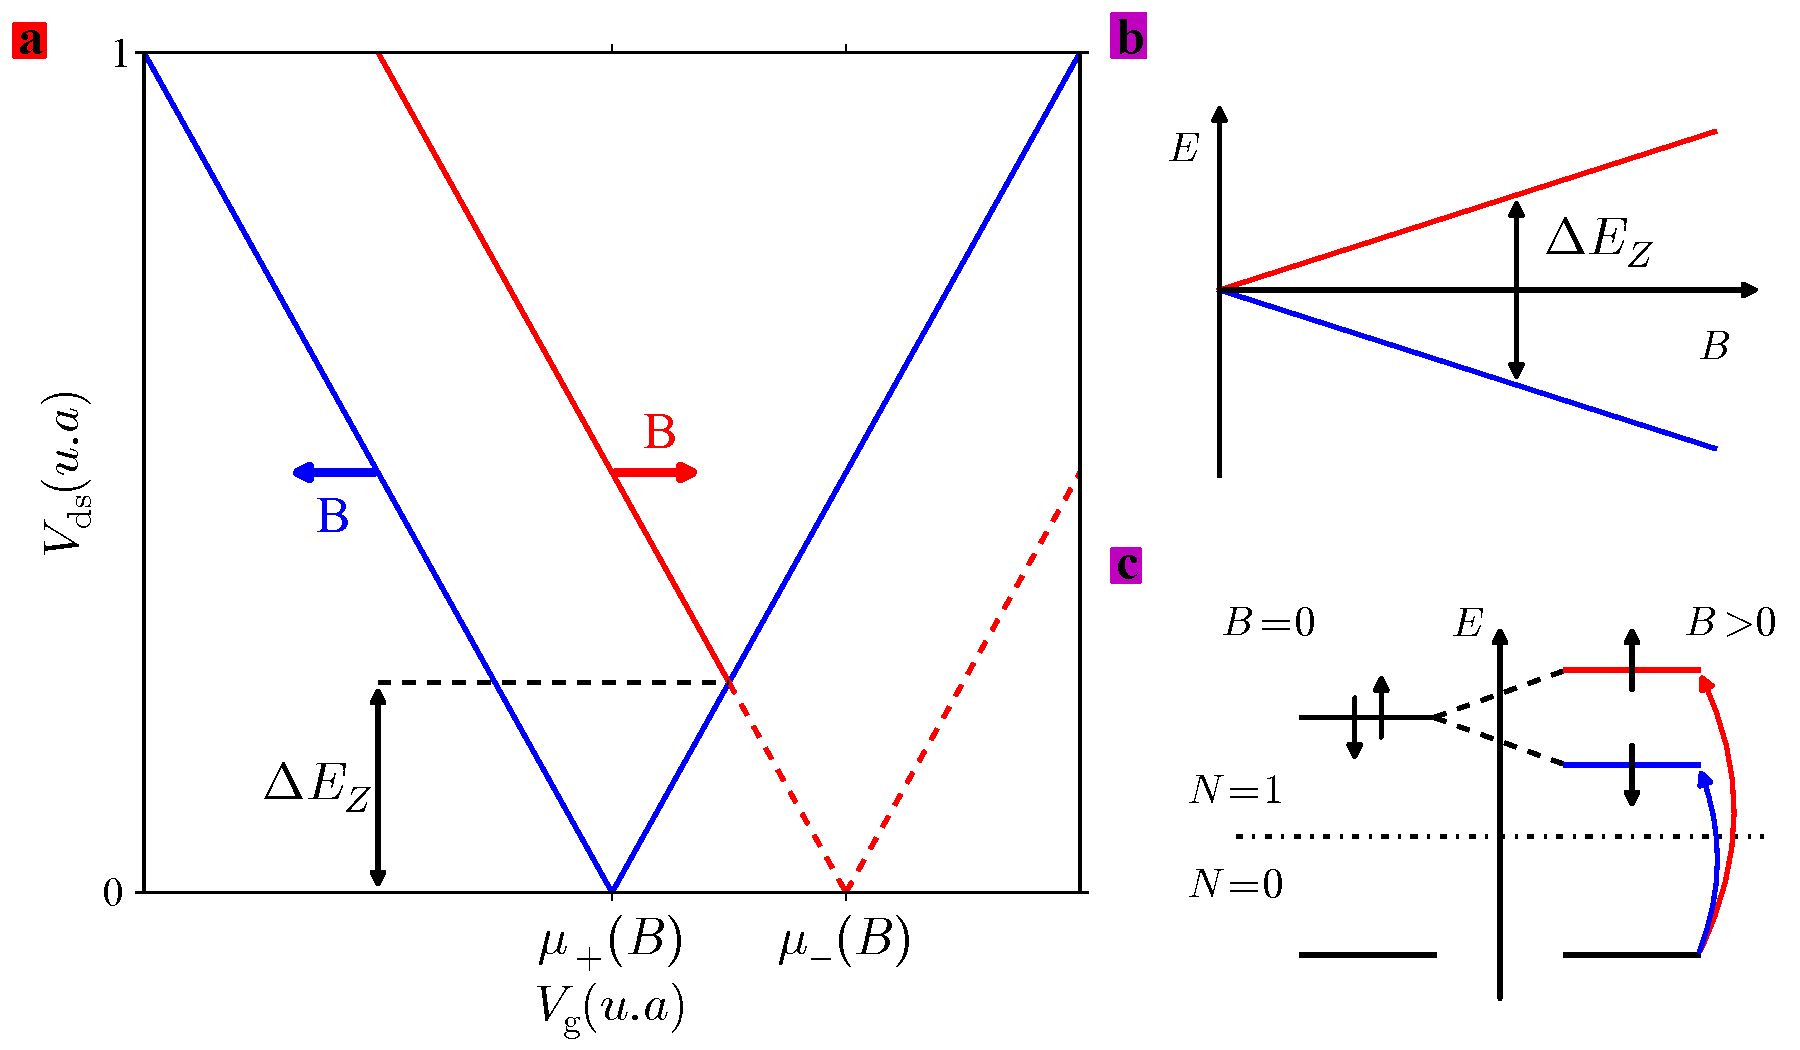
\includegraphics[scale=0.5]{Theorie/Transport/figure4/figure4.pdf} 
\caption{Diagramme Zeeman de l'état de charge N=1. Potentiel chimique correspondant à la transition 0/1}
\label{charge_discharge}
\end{figure}

\section{Cotunneling}
Nous avons vu jusqu'à maintenant que dans les zones de blocage de Coulomb, l'état de charge du système est fixe du fait de l'énergie de charge. En effet, l'ajout d'un électron supplémentaire aurait un "co\^ut" énergétique trop grand pour le système. Cependant, de part les inégalités d'Heinsenberg, un système peut outrepasser ce problème de "co\^ut" énergétique pendant un temps très court. L'ordre de grandeur de ce temps dépend de l'énergie nécessaire et est donné par la relation :
\begin{eqnarray}
\tau \simeq \frac{\hbar}{E_c} \nonumber
\end{eqnarray}


\begin{figure}
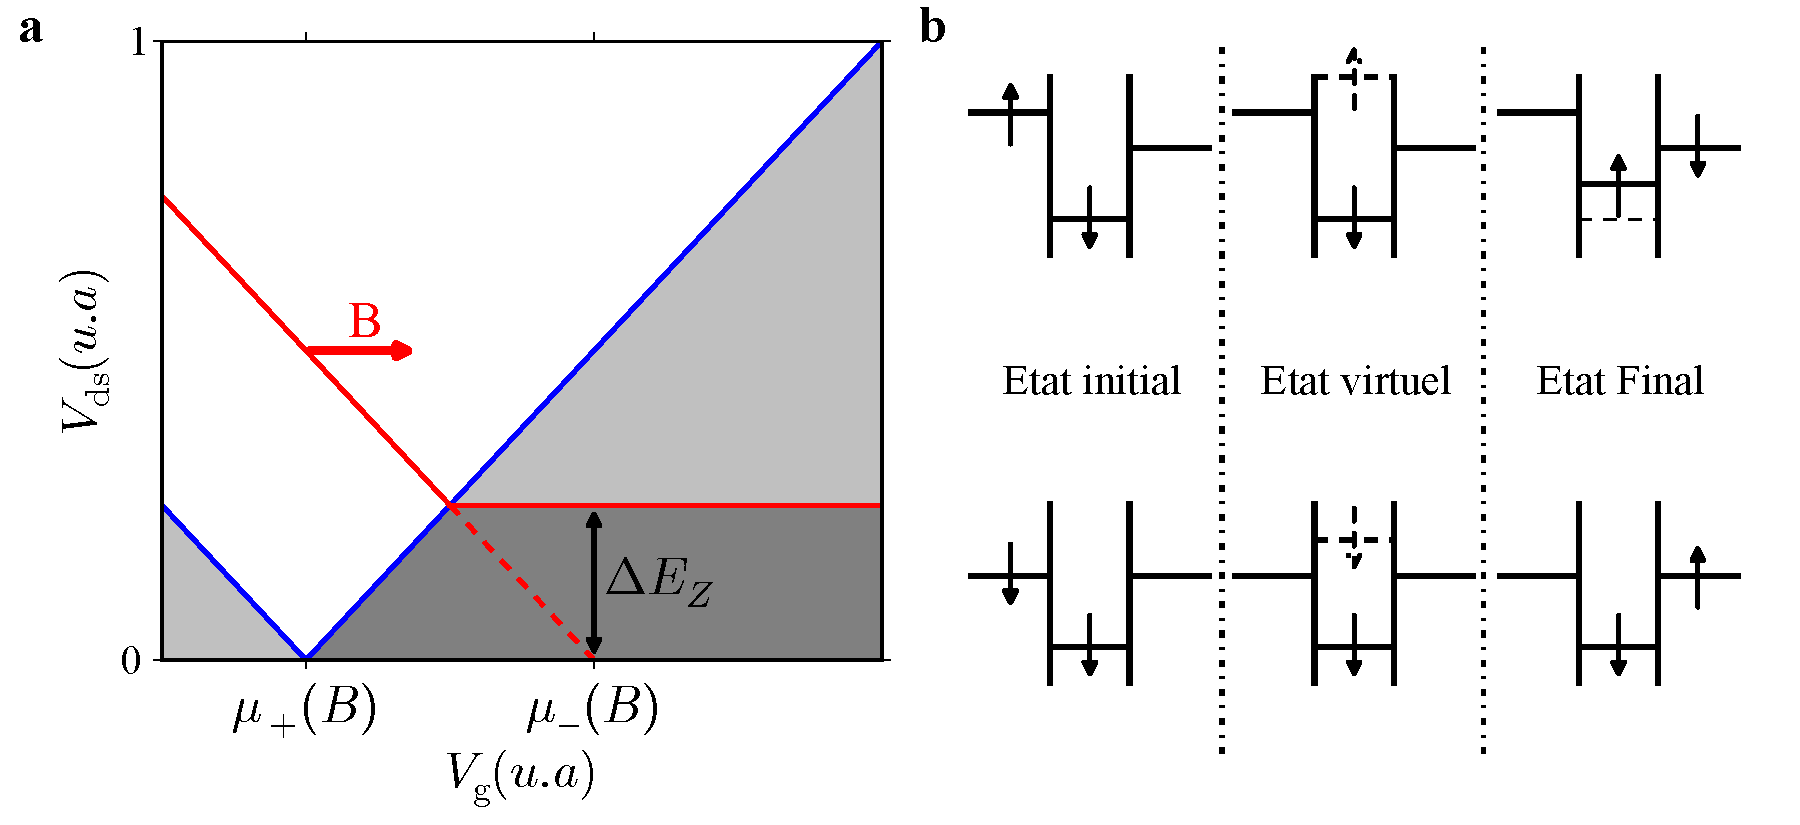
\includegraphics[scale=0.5]{Theorie/Transport/figure5/figure5.pdf} 
\caption{Représentation du cotunneling dans le plan ($V_g$,$V_{ds}$)}
\label{charge_discharge}
\end{figure}


Un façon de voir le phénomène est de dire que pendant le temps $\tau$ un électron est entré dans le point quantique pendant qu'un autre en est sorti. Si un m\^eme état de charge possède plusieurs états~(fondamentaux et excités), on peut imaginer deux situations. Dans le premier cas, l'électron entrant vient occuper un état de m\^eme énergie que celui de l'électron sortant et dans ce cas on parle de cotunnling élastique. L'électron entrant occupe un état d'énergie plus élevée que l'électron sortant et dans ce cas on parle de cotunneling inélastique. Dans le deuxième cas, cette différence en énergie que l'on notera $\Delta E_{cot}$ dans la suite doit être fournis au système. Dans notre cas, ce rôle est assuré par la tension $V_{\rm{ds}}$. Pour qu'un processus inélastique est lieu, il faut donc que :
\begin{eqnarray}
|e|V_{\rm{ds}} \geq \Delta E_{cot}
\end{eqnarray}

Dans le cas du cotunneling élastique cette condition est toujours remplie. C'est ce phénomène qui donne le fond de conductance mesuré dans les expériences de blocage de Coulomb. Plus intéressant encore, en faisant varier la tension de polarisation on peut venir sonder les différents état d'énergie pour un état de charge donnée.  Dans la zone de blocage de Coulomb, on va donc observer des zones avec des valeurs de courant différentes~(cf nuance de gris Fig.\ref{charge_discharge}.a). Dans le cas présenté ici, la limite entre les deux zones permet une lecture directe de l'effet Zeeman $\Delta E_z$. Encore une fois, il s'agit ici d'un cas simple avec seulement un état excité. Un étude plus complexe de la molécule endofullerène est présentée dans l'article en fin de thèse.\newline

\fbox{\begin{minipage}{0.9\textwidth}
\textbf{Remarque :} je voudrais ici insister sur la différence entre la spectroscopie en tunneling et celle en cotunneling. La première s'intéresse aux transitions entre des états relatifs à deux états de charges différents. Il faut donc "deconvoluer" le signal pour pouvoir analyser le spectre des deux états de charge. Dans le cas du cotunneling, on peut accéder directement aux spectres d'un état de charge donné. De part cette différence, les règles de sélection des transitions sont également différentes. Dans le cas du tunneling, on doit avoir $\Delta m = \pm 1/2$. Pour le cotunneling, cette règle de sélection devient $\Delta m = 0 \text{ ou } \pm 1$. Il peut arriver que des états inaccessibles par un spectroscopie en régime de tunneling soient en revanche accessibles par une mesure en régime de cotunneling. Une comparaison des deux méthodes peut \^etre trouvée dans l'article en fin de thèse ainsi que dans la thèse de Nicolas Roch.
\end{minipage}}


\section{Effet Kondo}

Tout comme le blocage de Coulomb, l'effet Kondo a d'abord été mesuré sur des échantillons macroscopique consistant en un metal massif contenant des impuretés magnétiques. En mesurant la conductance d'un tel échantillon, on avait constaté  qu'en dessous d'une certaine température la conductance avait tendance non plus à augmenter mais à atteindre un maximum pour diminuer à nouveau et tendre vers une limite inférieure à celle attendu par les modèles de l'époque. Ce problème est resté insoluble pendant quelques années jusqu'au modèle proposé par Jung Kondo en 1964. Ce modèle est relativement simple à concevoir mais en revanche très difficile à résoudre car faisant appel à la physique à $N$ corps. Dans ce modèle, les électrons de conduction viennent se coupler de façon antiférromagnétique aux impuretés du métal de telle sorte que le moment magnétique total devient nul. Chaque impureté agit donc comme un centre de diffusion très actif diminuant d'autant la conductance du système. La physique à $N$ corps apparait au travers des électrons de conduction. En effet, l'impureté magnétique n'interagit pas avec un seul électron du métal mais plutôt avec ce que l'on appelle un nuage Kondo. Il s'agit d'un phénomène hautement cohérent. Le seul problème du modèle à l'époque, c'est qu'il prevoit une divergence de la conductance quand la température tend vers zero. Il faudra attendre encore quelques années avec la théorie de renormalization proposée par Wilson, pour résoudre complètement le problème.

Ce problème est réapparu récemment dans ce que certain ont appelé "The revival of the Kondo Effect" (mettre la référence). La physique mésoscopique a permis de mettre à disposition des théoriciens des modèles bien plus simples à résoudre dans lesquels le nombre d'impuretés magnétiques pouvait être réduit à l'unité et également dans lequel le couplage aux électrons pouvait être contrôlé de manière précise. Les 2DEG par exemple permettent un contrôle quasi-parfait de ces différent paramètre. La littérature est riche en article et revues de toutes sortes couvrant de nombreux aspect de l'effet Kondo. Notre groupe à notablement contribuer à l'investigation de cette physique au travers notamment de l'étude de transition de phase et de Kondo sous écranté. Cependant, je ne traiterai pas en détail ici de ces effets.

\begin{figure}
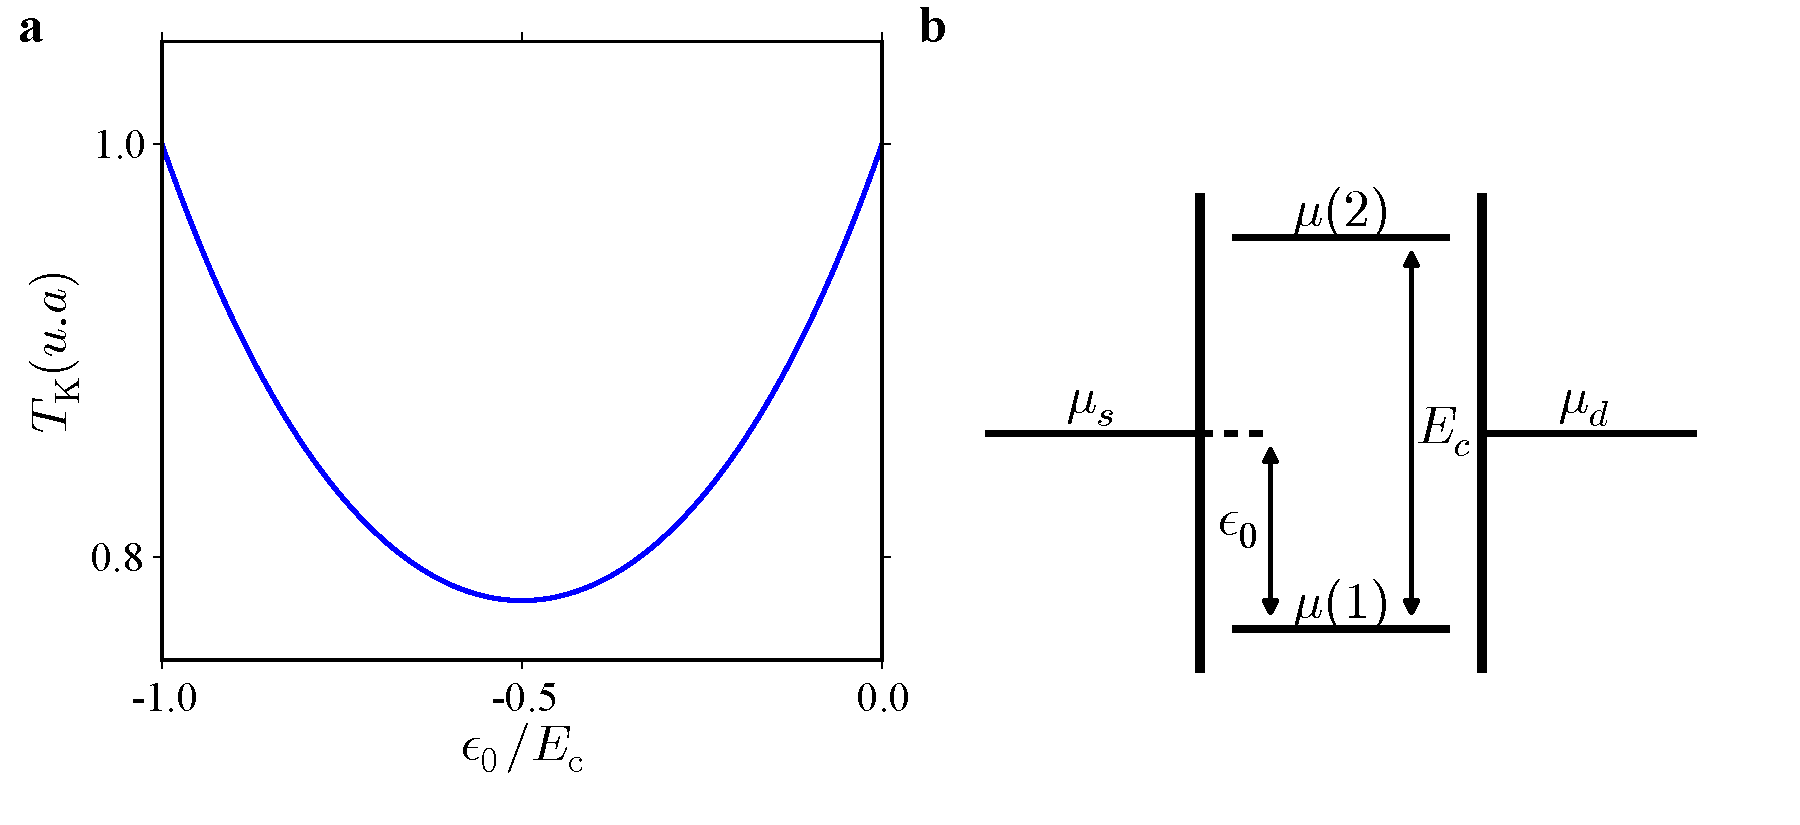
\includegraphics[scale=0.5]{Theorie/Transport/figure6/figure6.pdf} 
\caption{Kondo}
\label{Kondo_param}
\end{figure}


Je voudrait en revanche dresser quelques généralités de l'effet Kondo dans les transistors moléculaires. Comme je le disait précedemment, l'effet Kondo~(de spin) réside dans le couplage entre une impureté magnétique et les électrons de conduction. Dans notre système, cette impureté peut être jouée par un niveau ne contenant qu'un seul électron non apparié. Il s'agit donc d'une impureté de spin $1/2$. Cette impureté est couplée aux électrons de la source et du drain. Le couplage anti-ferromagnétique n'est effectif qu'en dessous d'une température caractéristique nommée température Kondo et noté $T_K$ dans la suite. Cette température $T_K$ dépend principalement de trois paramètres : l'énergie de charge $E_c$, le couplage aux électrodes $\gamma$ et la différence en énergie entre le potentiel chimique du point quantique et le niveau de Fermi des électrodes. Ces trois paramètres sont représentés sur la Fig.\ref{Kondo_param}.b et sont liés par la relation suivante:
\begin{eqnarray}
T_K \sim \frac{\sqrt{\gamma E_c}}{2} \exp(\frac{\pi \epsilon_0(\epsilon_0 + E_c)}{2\gamma E_c})
\end{eqnarray}

Première constatation, plus l'énergie de charge $E_c$ est grande plus la température Kondo sera élevée. C'est ici que réside un des avantages des transistors moléculaire comparativement aux 2DEGs. Les énergies de charge sont en général beaucoup plus élevé ce qui peut conduire à des $T_K$ de l'ordre de quelques dizaines de Kelvin. On remarque également que lorsqu'on s'éloigne d'un point de dégénérescence~(quand les trois potentiels chimiques sont alignés), $\epsilon_0$ augmente et donc la témpérature Kondo diminue pour atteindre son minimum au centre du diamant~(cf Fig.\ref{Kondo_param}.a). On peut donc moduler $T_K$ par l'intermédiaire de la grille.

De plus, l'effet Kondo se traduit dans nos structures par une augmentation de la conductance contrairement à ce qui avait été observé dans les matériaux massifs. En effet, la forte interaction des électrons de conduction avec le point quantique va grandement augmenter les évènements tunnels d'ordre plus élevé~(cotunneling d'ordre supérieur). Ceci peut être vu comme l'apparition d'une densité d'état dans l'ilôt alignée avec le niveau de Fermi des électrodes. Cela se traduit dans les mesures de transport par une conductance non nulle à tension source-drain proche de zéro à l'intérieur des zones des blocage. 

L'effet Kondo est sensible à des perturbations extérieures comme la tension source/drain~($E \sim eV_{\rm{ds}}$), la température~($E \sim k_bT$) ou bien encore le champ magnétique~($E \sim g \mu_bB$). On peut discerner deux régimes :
\begin{itemize}
\item $E \ll k_bT_K$ : dans ce cas, la conductance est donnée par $G(E) = G_0(1-C (E/k_bT_K))^2$, $C$ étant un nombre qui dépend de la perturbation appliquée au système ainsi que de la géométrie du système.
\item $E \gg k_bT_K$ : on obtient la dépendance suivante : $G(E) = 1/\ln^2(E/k_bT_K)$. C'est ce régime qu'avait décrit Kondo.
\end{itemize}
Afin de décrire le régime intermédiaire, il est nécessaire de faire appel à la technique du groupe de renormlization numérique, NRG en anglais. Nous verrons dans la partie résultat comment cette sensibilité aux perturbations peut \^etre utilisé pour évaluer l'énergie d'interaction des électrons du point quantique avec un moment magnétique proche.
\chapter{Le Magnétisme Moléculaire}

Pour classer une molécule en tant qu'aimant moléculaire, il faut qu'elle possède un moment magnétique non nul. Celui-ci peut \^etre de spin, orbital ou bien les deux. Il faut de plus, que ce moment magnétique est une orientation préférentielle. Cela se traduit par l'existence d'un axe facile, c'est à dire deux orientations qui correspondent à un minimum d'énergie. Ces deux conditions sont les conditions minimales à remplir pour parler d'aimant moléculaire. Mais pour mettre en évidence ces propriétés, il faut qu'il soit possible de les mesurer. Autrement dit, l'anisotropie doit \^etre suffisamment forte pour que l'énergie thermique ne puisse pas retourner l'aimantation.

Cependant, l'aimant moléculaire que l'on vient de décrire n'est pas vraiment "sexy" pour reprendre les termes de Wolfgang Wernsdorfer. Ce que l'on souhaite aussi, c'est pouvoir mettre en évidence des phénomènes quantiques tel que le retournement de l'aimantation par effet tunnel~(ou Quantum Tunneling of the Magnetization - QTM) ou bien encore la phase de Berry. Ceci n'est possible que s'il existe, en plus de l'axe facile, un plan difficile. En effet, comme nous le verrons dans la suite, la presence d'un plan difficile entraîne un couplage entre les différents états magnétique de la molécule.

De plus, le spin électronique n'est pas toujours l'unique acteur du magnétisme moléculaire. Il arrive parfois que le spin nucléaire, au travers du couplage hyperfin, joue un r\^ole majeur dans les phénomènes quantique et les propriétés magnétiques mesurés.

Afin de comprendre la physique associé aux aimants moléculaires, on peut donc procéder par étape. On peut tout d'abord décrire l'origine physique du moment magnétique d'une molécule. On peut ensuite introduire la notion d'axe facile et voir comment cette notion se traduit dans le formalisme quantique. On peut ensuite aborder la notions de plan difficile, son origine et ces conséquences. Enfin, une description des interaction entre spin électronique et spin nucléaire est nécessaire pour décrire de la façon la plus complète certains aimants moléculaire, à base de lanthanide notamment.

\section{L'origine du moment magnétique}
Nous l'avons déjà dit, pour qu'une molécule puisse \^etre appelé aimant moléculaire, il faut tout d'abord qu'elle possède un moment magnétique non nul. Pour arriver à ce résulat, on peut adopter deux stratégies. La première consiste à synthétiser une molécule composé de plusieurs atomes magnétique qui vont interagir entre eux, par l'intermédiaire des ligands, pour donner un moment magnétique résultant non nul. La deuxième technique consiste à n'utiliser qu'un atome métallique magnétique que l'on va venir entourer de ligands non magnétiques.

\subsection{La solution a plusieurs centres}
Cette solution a été la première adopté dans le domaine du magnétisme moléculaire. Elle a permis notamment de synthétiser la désormais célèbre molécule de Mn$_{12}$-ac~(cf Fig.\ref{Mn12}). Cette dernière est composé de douze atomes de Manganèse et autant d'atomes d'oxygène~(qui consituent le coeur magnétique) ainsi que des ligands organiques. Les huit atomes de manganèse en périphérie, de part leur interaction, sont parallèles les uns au autres. Chacun d'eux possédant un spin $S=2$, on se retrouve avec un spin total $S=16$. Les trois atomes situés au centre du coeur magnétique sont également alignés entre eux pour un spin total de $S=6$~(pour chaque manganèse $S=3/2$). Ces deux groupes étant antiparallèle l'un par raport à l'autre, on obtient un spin total de $S=10$. Dans cet exemple, les atomes d'oxygène jouent un r\^ole majeur au travers de l'interaction dite de "super échange" qui lie les différents atomes de manganèses entre eux.
\begin{figure}
\centering 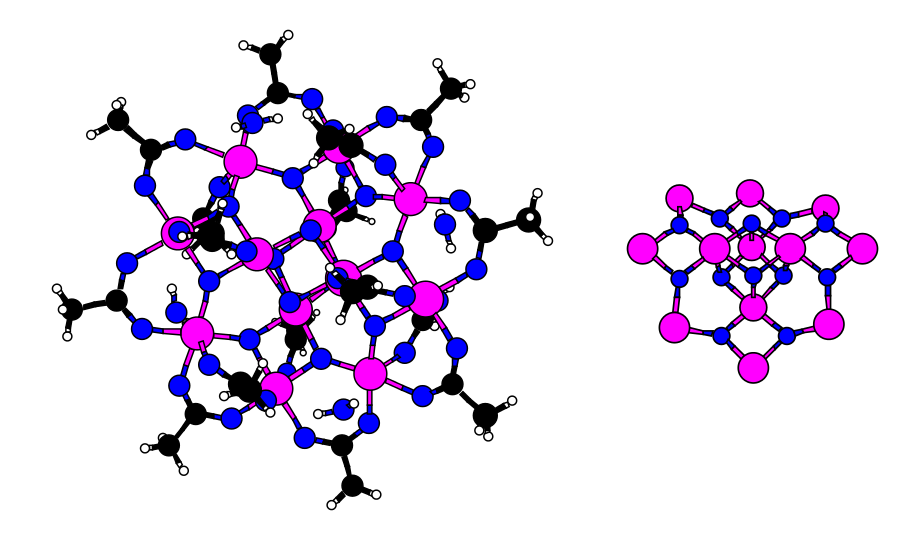
\includegraphics[scale=0.3]{Theorie/MagMol/figure1/Mn12.png} 
\caption{Sur la gauche, la molécule de Mn$_{12}$-ac. Sur la droite, le centre magnétique Mn$_{12}$O$_{12}$. Les quatre manganèses internes de spin $S=3/2$ sont antiparallèles aux huit maganèses de spin $S=2$ situés en périphérie. Le moment magnétique total résultant est $S=10$~(extrait de When Magnetism Goes Nano). Le couplage entre les différents spins est médié par les atomes d'oxygène en bleus sur la figure.}
\label{Mn12}
\end{figure}

\subsection{La solution de l'ion métallique unique}
Dans ce deuxième type d'aimants moléculaires, le moment magnétique total ne dépend que de celui de l'ion qui la compose. Cet ion va \^etre ensuite inséré dans un ligand pour former un aimant moléculaire. Contrairement à ce qui a été présenté précédemment, le moment magnétique total ne dépend donc pas des interactions entre différents centre magnétique. On peut dors et déjà y voir un signe de robustesse, ce type d'aimant moléculaire étant par construction, moins sensible à une déformation de sa structure~(cf chapitre précédent avec l'effet Jhan-Teller). Parmis les molécules les plus étudiées , on trouve le "double-decker"~(nommé en référence aux avions à deux ailes) où plusieurs ion peuvent \^etre choisi comme centre magnétique. Dans notre cas, nous utiliserons le TbPc$_2$ où terbium "double-decker".

\begin{figure}
\centering 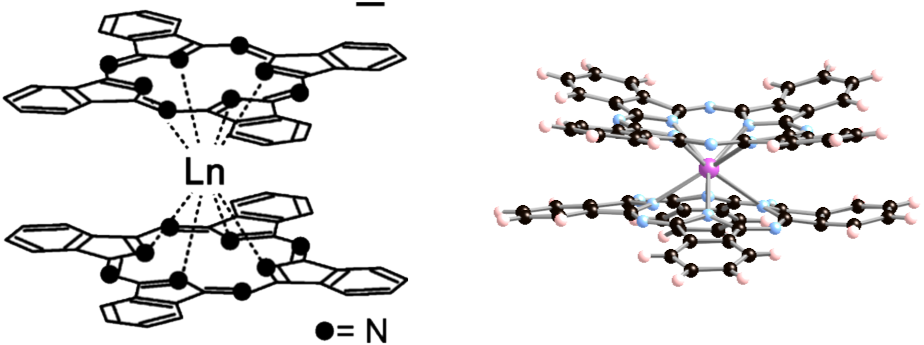
\includegraphics[scale=0.5]{Theorie/MagMol/figure2/figure2.png} 
\caption{A gauche, structure générale d'un "double decker" à base de Lanthanide~(noté Ln - tiré de Ishikawa, Single molecule magnet with single lanthanide ion). A droite, vu d'artiste de cette m\^eme molécule. Les atomes d'azote sont représentés en bleu, ceux de carbone en noir, ceux hydrogènes en beige et l'atome lanthanide en mauve}
\label{TbPc2}
\end{figure}

\section{Hamiltonien d'un aimant moléculaire "standard"}
\subsection{L'axe facile}
Comme nous le disions plus haut, le ligand a aussi une influence sur le magnétisme de la molécule. Cette influence peut \^etre prise en compte par l'introduction d'un champ de ligand. Son origine est purement Coulombienne
 et dépend très fortement des symétrie du système. On utilise pour rendre compte de ce phénomène les opérateurs de Stevens rappelé en annexe. Pour notre introduction, nous allons nous concentrer sur le terme le plus simple qui peut introduire un axe facile à savoir:
 \begin{eqnarray}
E_{ani} = -DS_z^2 \nonumber
\end{eqnarray}
où $D$ est le paramètre d'anisotropie, $S_z$ la composante en $z$ du moment magnétique et $E_{ani}$ la modification de l'énergie du système du à cette anisotropie. Si $D>0$, nous avons à faire à un axe difficile et le moment magnétique se trouvera de préférence dans le plan perpendiculaire à l'axe $z$. Si $D<0$, nous avons un axe facile et le moment magnétique sera aligné le long de l'axe z.

\subsection{Le plan difficile}
De m\^eme que nous pouvons avoir un axe facile( ou difficile), on peut égalment rencontrer un plan difficile(~ou facile). Il peut \^etre exprimé deux façons rigoureusement équivalente :
\begin{eqnarray}
E_{plan} = E ( S_x^2 -S_y^2) \nonumber
\end{eqnarray}
ou bien encore
\begin{eqnarray}
E_{plan} = \frac{E}{2} ( S_+^2  + S_-^2) \nonumber \\
\end{eqnarray}
où $S_x$ et $S_y$ sont les projection du moment magnétique dans le plan $(x,y)$, $S_+$ et $S_-$ les opérateurs création anhilation, $E$ est le paramètre d'anysotropie et $E_{plan}$ l'énergie associé à la présence d'un plan difficile. La présence des termes création anhilation n'est pas sans conséquence sur le système. En effet, ces termes vont venir coupler les différentes valeur $m_z$. On verra plus tard quelles sont les conséquences d'un tel couplage.

\subsection{L'effet Zeeman}
Comme tout système magnétique, un aimant moléculaire est sensible au champ magnétique. Celui si va venir faire varier l'énergie du système de la valeur
\begin{eqnarray}
E_{Zeeman}= g\mu_b \mathbf{BS} \nonumber
\end{eqnarray}
ou $E_{Zeeman}$ est l'énergie associé à l'effet Zeeman, $g$ le facteur de Landé, $\mu_b$ le magnéton de Bohr, $B$ le champ magnétique appliqué et $S$ le moment magnétique du système. Si maintenant ce champ magnétique est appliqué celon l'axe $z$ du système, cette expression devient :
\begin{eqnarray}
E_{Zeeman}= g\mu_b B S_z \nonumber
\end{eqnarray}

\subsection{La cas du Fe$_8$}
Si l'on synthétise ce qui vient d'\^etre présenté, un aimant moléculaire soumit à un champ magnétique $B$ appliqué suivant l'axe $z$ possède l'hamiltonien suivant:
\begin{eqnarray}
E =  -DS_z^2 + \frac{E}{2} ( S_+^2  + S_-^2) + g\mu_b B S_z 
\end{eqnarray}


Nous allons maintenant appliqué cet hamiltonien à l'étude d'un aimant très utiliser dans les expériences relativer au magnétisme moléculaire : le Fe$_8$. Nous avons déjà vu l'influence de l'effet Zeeman et de l'axe facile sur les spectre en énergie d'un système. Ici, nous allons nous intéresser plus particulièrement à la présence d'un plan difficile est voir comment se plan vient perturber le système. Nous avons donc tracer le diagramme Zeeman de la molécule de Fe$_8$ en ne tenant pas compte de la présence d'un plan facile et ensuite en l'introduisant dans l'hamiltonien du système. On constante tout d'abord une altération forte de l'allure générale du diagramme Zeeman. Mais plus important que cela, nous voyons apparaitre des zones où, au lieu de se croise, les niveaux d'énergie ont l'air de "s'éviter" : on parle d'anti-croisement. La présence de ces anti-croisements témoigne du couplage entre les différents état de l'aimantation du système. Nous allons à present étudier les conséquence d'un tel couplage.

\subsection{les anti-croisement}
Au niveau d'un anti-croisement, les états propres du système ne sont plus les états magnétique ($S,S_z$) mais plutot une combinaison de ces états. Si l'on se place loin de l'anti-croisement, les états $m$ et $m'$ sont les états propre du système. Mais plus on se rapproche de l'anti-croisement plus les états sont mélange pour anteindre un maximum d'intrication quand la séparation en énergie entre les deux niveau est minimale.

Lorsque l'on balaie le champ magnétique autour d'un tel anti-croisement, il y a une certaine probabilité de passer de l'état $m$ à l'état $m'$ et vice-versas. Cette probabilité est régie par la formule de Landau-Zenner qui dépend à la fois de la séparation minimale entre les deux niveaux ainsi que de la vitesse de balayage du champ magnétique. Cette probabilité peut s'exprimer de la façon suivante :
\begin{eqnarray}
P = 1 - \exp \left( -\frac{\pi \Delta^2_{mm'}}{2 \hbar g \mu_B |m-m'|\frac{dH_z}{dt}} \right)
\end{eqnarray}
ou P est la probabilité de passer de l'état $m$ à l'état $m'$, $\Delta_{mm'}$ l'écart minimum en éngergie entre les deux niveaux, $\frac{dH_z}{dt}$ la vitesse de balayage en champ magnétique. On constate tout d'abord que si la vitesse est très faible, la probabilité de passer d'un état à l'autre est de 1. On retrouve ici le théorème adiabatique. A l'autre bout de l'échelle, si je balaie très rapidement le champ magnétique cette probabilité devient nulle. Tout se passe comme si l'on avait été si vite que le système n'avait pas eu le temps de "sentir" l'anti-croisement.

\section{Le Terbium double-decker ou TbPc$_2$}

\subsection{Origine du moment magnétique}
Le terbium double-decker est un aimant moléculaire dont le moment magnétique est d\^u à un centre magnétique unique : l'ion Tb$^{3+}$. L'atome de Terbium possède un noyau relativement lourd et le couplage spin orbite joue donc un r\^ole prépondérant dans les propriété magnétique de ce dernier. Le moment magnétique fondamental total de cet ion peut \^etre déterminer par un calcul relativement complexe. La théorie donnent un moment total $J=6$ pour l'état fondamental ainsi qu'une séparation en énergie de plusieurs millier de Kelvin entre celui-ci et le premier état excité $J=5$. On peut donc sans trop de risque négliger les états excité et considéré uniquement la configuration $J=6$. Ce moment provient du moment angulaire électronique~($L=3$) ainsi que des six spins électroniques non appariés. 

\subsection{Hamiltonien}

\subsubsection{Le moment magnétique électronique}
L'Hamiltonien relatif au TbPc$_2$ est beaucoup plus complexe que ce qui a été présenté précédemment. Il est pour cela plus pratique de faire appel aux opérateur de Stevens afin d'obtenir une écriture plus concise. Cependant et de la même manière, on peut discerner une composante relative à l'axe facile et une seconde relative au plan difficile. 

En ce qui concerne l'axe facile, l'Hamiltonien correspondant est le suivant :
\begin{eqnarray}
H = \alpha A_2^0 \langle r^2 \rangle O_2^0 + \beta A_4^0 \langle r^2 \rangle O_4^0 + \gamma A_6^0 \langle r^2 \rangle O_6^0
\end{eqnarray}
ou les différent $O_i^0$ sont les opérateurs de Stevens, $A_i^0$ les coéfficient relatifs à la molécule de TbPc$_2$ et $\alpha$, $\beta$ et $\gamma$ les coéfficient introduit par Stevens. Les opérateur $O^0_i$ sont basé sur des sommes d'opérateur $S_z^{2n}$. Il s'agit donc d'un opérateur diagonal qui ne vient pas coupler les différents état de la base ($J$,$J_z$) entre entre eux. Le diagramme Zeeman correspondant est donné dans la Fig. ??.a.

Si l'on s'arr\^etre un temps sur les échelles d'énergie, on constate que les états fondamentaux $J_z = \pm 6$ sont isolé des états excités par une énergie de plus de $400$\,K. Puisque nos expérience se font dans le domaine du sub-Kelvin, on peut dans notre trairement négliger les états excité et nous concentrer sur les deux états fondamentaux  $J_z = \pm 6$.

Si l'on veut tenir compte de la présence d'un plan difficile, il faut introduire un dernier terme dont la forme est
\begin{eqnarray}
H = \beta A_4^4 \langle r^2 \rangle O_4^4
\end{eqnarray}
où la m\^eme notation a été utilisé. Ce dernier terme ne modifie pas l'allure générale du diagramme Zeeman. En revanche, il introduit un couplage entre les états  $J_z = \pm 6$. On observe donc des anti-croisement comme le montre la figure ??.b.

\subsubsection{Le spin nucléaire}
Les orbitale électronique étant de type 4f, leur interaction avec le spin nucléaire doit \^etre prise en compte. Dans le cas du terbium, le spin nucléaire est de $I = 3/2$. Du fait de ça forme allongé, il possède élgalement un moment quadripolaire de sorte que l'hamiltonien relatif au spin nucléaire est donné par :
\begin{eqnarray}
H_I = P\left(I_z^2 - \frac{1}{3}I(I+1)\right)
\end{eqnarray}
où $P$ est le moment quadripolaire et un terme constant a été ajouté pour garder le barycentre des énergie sur zéro.

De plus, cet spin nucléaire interagit avec le moment magnétique électronique au traver de l'interaction hyperfine. Un terme rendant compte de cette interaction doit donc \^etre introduit pour tenir compte de cette interaction. Son expression est simple et ne met en jeux que le produit scalaire des deux spin :
\begin{eqnarray}
H_{hf} = A_{hf}\mathbf{J}\mathbf{I}
\end{eqnarray}
où $\mathbf{J}$ et $\mathbf{I}$ sont respectivement le moment magnétique électronique et le spin nucléaire, $A_{hf}$ étant la constante d'interaction hyperfine.

\subsubsection{L'Hamiltonien de l'aimant moléculaire}

Ces différents terme doivent bien s\^ur \^etre inclus dans l'Hamiltonien total de l'aimant moléculaire. Cela donne, en reprenant la notion précédente
\begin{eqnarray}
H =&& \alpha A_2^0 \langle r^2 \rangle O_2^0 + \beta A_4^0 \langle r^2 \rangle O_4^0 + \gamma A_6^0 \langle r^2 \rangle O_6^0 + \beta A_4^4 \langle r^2 \rangle O_4^4 \\ \nonumber
 &&+ A_{hf}\mathbf{J}\mathbf{I} + P\left(I_z^2 - \frac{1}{3}I(I+1)\right)
\end{eqnarray}
Les trois derniers terme n'agissent que comme une perturbation et l'allure générale présenté dans la figure??.a n'est pas altéré. On peut donc continuer à ce concentrer sur les seuls états $J_z = \pm 6$. A cette échelle en revanche, les effets ne sont plus négligeable. En plus de l'anti-croisement introduit par la présence du plan difficile, le couplage hyperfin vient diviser les états fondamentaux  $J_z = \pm 6$ en deux jeux de quatre états, chacune de ces quatre états étant relatif à un état de spin nucléaire. De plus, pour un m\^eme état de spin nucléaire, l'anti-croisement entre les états de  $J_z = \pm 6$ sont conservé. En revanche, seul des croisements sont observés pour les état de spin nucléaire différents. Ceci est clairement visible sur le diagramme Zeeman présenté dans la figure??.

%\part{Résultats}

\chapter{Chapitre 1}

\section{Le couplage en transport : du direct à l'indirect}

Lorsque l'on souhaite sonder le magnétisme moléculaire par une mesure en courant, il faut que le "chemin" emprunté par les électrons soient très proche du centre magnétique. On peut, dans ce cadre, imaginer deux configurations : le couplage direct, où les électrons impliqués dans le transport jouent également un rôle direct dans le magnétisme de la molécule sondée; le couplage indirect, dans lequel les électrons impliqués dans le courant ne contribue pas au magnétisme de la molécule, mais le perturbe légèrement. Suivant la configuration adoptée, le mode de mesures sera différent, tout comme le sera l'impact sur le magnétisme. C'est ce que nous allons détailler maintenant.

\subsection{Le couplage direct}
Nous l'avons vu, le couplage direct implique que les électrons responsable du courant jouent également un rôle dans le magnétisme de la molécule. Cette dernière va osciller entre deux états de charge N/N+1 , chacun d'eux ayant sa propre configuration magnétique. L'analyse se fait en sondant la différence en énergie des différentes transitions N/N+1, le plus souvent par une technique de spectroscopie en tunnelling séquentiel. Le principal avantage de cette technique est qu'elle permet d'étudier différents états de charge~(nombre d'oxydation ou de réduction). En revanche, le caractère très invasif de la méthode ne permet pas d'espérer de long temps de vie pour les différents états du système. Cette méthode a été mise en œuvre expérimentalement dans [mettre les citations] avec des résultats mitigés, du fait notamment de la dégradation de la molécule lors de la fabrication du dispositif. Des études théoriques ont également été menée, permettant une analyse plus fine des résultats expérimentaux.

\subsection{Le couplage indirect}

Dans le cas du couplage indirect, les électrons responsables du courant ne participent qu'indirectement au magnétisme de la molécule. Le couplage à l'origine de cette interaction sera détaillé dans la suite. La mesure se fait par l'analyse statistique des modifications de conductance du système, la polarisation en tension source-drain et grille étant en général fixée~(par opposition à la spectroscopie en tunneling séquentiel). Dans ce cas, il n'y a pas de possibilité de modifier le nombre d'électron impliqués dans le magnétisme moléculaire. En revanche, la technique de mesure par couplage indirect se révèle beaucoup moins invasive. Cela garantie d'une part, la préservation des propriétés magnétique et d'autre part, l'observation de long temps de vie. Cette configuration a été utilisé dans deux dispositifs légèrement différents. Dans le premier, une deuxième molécule~(un nanotube) a été utilisé comme point quantique sonde, l'aimant moléculaire étant déposé sur sa surface [citation de Matias]. Dans le deuxième dispositif, le cœur magnétique étant fortement découplé des ligands périphériques, ces derniers ont joué le role de point quantique sonde[nous]. Quelques outils théoriques sont venu également faciliter l'interprétation des résultats [papier sur nanotube] mais également proposer de nouvelle expérience [article du les ligand et couple mécanique].

\section{Le couplage magnétique}
Dans la configuration directe présenté précédemment, le couplage entre le courant et le magnétisme est aisé à comprendre, les électrons participant au premier étant également directement impliqué dans le second. En revanche, dans la configuration indirecte, le couplage entre les ces deux domaines peut avoir plusieurs origines. Il a pour conséquence de rendre le potentiel chimique du point quantique dépendant du centre magnétique. Cette dépendance est fonction de la nature de l'interaction comme nous allons le montrer maintenant.

\subsection{Origine dipolaire}
Le couplage dipolaire est une interaction à distance entre deux moments magnétique. Chacun de ces moments génère un champ dipolaire qui va venir agir sur le second, et vice versa. La modification en énergie induite est fonction de la distance séparant les deux dipôles, ainsi que de leur orientation relative. Ceci s'exprime par:
\begin{eqnarray}
E = -\frac{\mu_0 \mu_B}{4\pi r^3}(3\mathbf{SnJn} - \mathbf{SJ}) \nonumber
\end{eqnarray}
où S et J sont les spins associés au deux moment magnétiques, r la distance qui les sépare et n la normale reliant les deux moments (cf figure??). Plusieurs remarques s'imposent. Premièrement, l'intensité de l'interaction est proportionnelle à l'inverse de la distance au cube. Elle devient très rapidement négligeable : pour un spin J=6, elle ne vaut plus que 10\,mT à 1\,nm. Deuxièmement, on peut imaginer deux configurations extrème : dans la situtation de la figure??, le couplage abouti à une organisation anti-ferromagnétique; dans celle présenté dans la figure ??, le couplage est au contraire ferromgnétique. Dans le cas de TbPc2, le plan des ligands est perpendiculaire à l'axe facile du moment magnétique. Cela correspond plutôt à la seconde configuration. De plus, la seule transition possible à basse température est $J_z=\pm6 \rightarrow J_z \mp 6$. Si l'on tient compte de ces remarques, la variation du potentiel chimique du point quantique sonde $\mu_{QD}$, est lié au renversement du moment magnétique par :
\begin{eqnarray}
\Delta \mu_{QD} = -\frac{\mu_0 \mu_B}{2\pi r^3}S_z\Delta J_z\nonumber
\end{eqnarray}

Celle-ci est directement proportionnelle à $\Delta J_z$. Autrement dit, le retournement du moment magnétique entraîne une variation de potentiel chimique constante.

\subsection{Couplage d'échange}
Le couplage d'échange est une interaction de contact entre deux moments magnétiques. Elle résulte d'un recouvrement des fonctions d'onde et peut favoriser deux situations opposés : si les spin s'alignent entre deux, elle est de type ferromagnétique; si l'orientation entre spin est opposée, elle est de type anti-ferromagnétique. Cette interaction s'exprime comme suit :
\begin{eqnarray}
E = A\mathbf{SJ} \nonumber
\end{eqnarray}
où A est la constante d'échange. Lorsque $A>0$, le couplage est anti-ferromagnétique, si $A<0$ il est ferromagnétique. La constante d'échange peu prendre des valeurs élevées en énergie : dans le cas du N@C$_{60}$ par exemple, la valeur de l'échange entre le spin de l'azote et les électrons du C$_{60}$ a été mesurée supérieure à 4\,T. Si l'on tient compte des même considération que dans le cas du couplage dipolaire, la modification d\^u à l'interaction d'échange qu’entraîne un retournement de l'aimantation peut s'exprimer de la façon suivante :
\begin{eqnarray}
\Delta \mu_{QD} = AS_z\Delta J_z\nonumber
\end{eqnarray}
Cette expression est semblable à celle obtenue pour le couplage dipolaire. Dans le cas où $A<0$ , les deux interactions produisent même des effets identiques. La principale différence se fait par l'intensité de l'interaction : si celle-ci n'est que de l'ordre du mT, elle est certainement dipolaire; si elle est en revanche de l'ordre de quelques dizaine de mT, l'interaction d'échange est l'interaction dominante.

\subsection{Le couplage magnéto-Coulomb}
L'origine de ce couplage est électrostatique. Si l'on considère un point quantique et un centre magnétique, cette interaction va coupler le potentiel chimique du premier à celui du second de telle sorte que :
\begin{eqnarray}
\Delta \mu_{QD} = C_{mc} \Delta \mu_{CM}
\end{eqnarray}
où $C_{mc}$ est la constate de couplage et $\mu_{CM}$ la variation du potentiel chimique du centre magnétique. Cette expression peut être simplifier, au regards des remarques précédentes, de la façon suivante :
\begin{eqnarray}
\Delta \mu_{QD} = C_{mc} g \mu_B  \Delta J_z B_z
\end{eqnarray}
Contrairement aux expressions précédentes, la variations du potentiel chimique associée à un retournement de l'aimantation n'est pas constante mais dépend du champ magnétique appliqué. Cela rend cette dernière facile à identifier dans nos mesures.

\section{Nature et intensité de l'interaction}
L'analyse de nos résultats passe par la détermination l'identification de l'interaction mise en jeu dans notre méthode de détection, à savoir, les sauts de conductance. Deux paramètres sont à évaluer pour clairement en identifier la nature : la dépendance en champ magnétique de la variation du potentiel chimique et l'intensité de l'interaction. Nous allons nous attacher à quantifier ces deux paramètres à l'aide de mesure en transport. La première étape sera consacré à l'étude de la hauteur des sauts de conductance. La seconde s'appuiera sur une étude de l'effet Kondo et sur l'influence de l'interaction sur ce dernier.

\subsection{Amplitude du saut de conductance}
Dans le chapitre théorique, nous avons montré que le potentiel chimique du point quantique était directement relié à la conductance différentielle mesurée. On peut résumer cette tendance par la relation suivante:
\begin{eqnarray}
\text{d}G = \frac{\partial G}{\partial \mu} \text{d} \mu
\end{eqnarray}
Si l'on se place dans une situation où $\frac{\partial G}{\partial \mu} = cst$, alors la variation observée en conductance sera une mesure directe de la variation du potentiel chimique. Si maintenant, on considère la variation du potentiel chimique en fonction du champ magnétique, sans renversement magnétique, on a $\text{d}\mu \propto \text{d}B$. Pour avoir $\frac{\partial G}{\partial \mu} = cst$, cela revient à se placer dans une zone ou $\frac{\partial G}{\partial B} = cst$. La Fig.??? montre une mesure de $G$ en fonction du champ magnétique $B$ et met en évidence la zone correspondante à $\frac{\partial G}{\partial B} = cst$. Dans celle-ci, un saut en conductance est directement proportionnel à la variation en potentiel chimique. Si cette dernière est dépendante en champ magnétique, la hauteur des sauts en conductance devrait également l’être. Or, la mesure présenté dans Fig.?? montre clairement que la hauteur des sauts en conductance ne varie pas en fonction du champ magnétique. Cette première observation nous permet d'éliminer l'interaction de type magnéto-Coulomb des mécanismes de coulage possible. On a donc à faire, soit à un couplage dipolaire, soit à un couplage d'échange. Seul l'analyse de l'intensité de l'interaction peut nous renseigner et c'est à sa détermination que nous allons nous attacher maintenant.

\subsection{Intensité de l'interaction}
L'intensité de l'interaction peut s'obtenir en comparant un système découplé de l'interaction avec le même système la subissant. Pour cela, on peut s'appuyer sur un phénomène universel tel l'effet Kondo de spin 1/2.

\subsubsection{L'effet Kondo 1/2}
La Fig??? présente la mesure d'un effet Kondo 1/2 en fonction du champ magnétique et de la tension source drain. A $B=0$, on observe un pic de conductance à $V_{ds}=0$. Lorsque l'on applique un champ magnétique, ce pic s'étale puis, puis se divise en deux pics de conductance. Cette séparation est directement induite par l'effet Zeeman. En extrapolant les maxima pour different B, on obtient une lecture de l'écartement Zeeman. En revanche, contrairement à ce que l'on pourrait attendre, les droites ne se croisent pas en $B=0$, mais en une valeur de champ fini $B_c$ supérieur à zéro. La valeur de $B_c$ est directement relier à la température Kondo $T_K$ par $k_bT_K = \mu_B B_c$. Cela traduit qu'il est nécessaire de fournie une énergie supérieur à celle de la température Kondo pour "casser" le singlet formé par le nuage Kondo et l'électron du point quantique. Regardons maintenant ce qu'il en est de notre système couplé.

\subsubsection{Effet Kondo du système couplé}
Si l'on effectue cette étude dans le cas du Kondo 1/2 couplé, on observe le même comportement général. Les pentes des droites extraites des extrema confirme qu'il s'agit d'un Kondo de spin 1/2. En revanche, la valeur de $B_c$ n'est plus positive mais négative. Tout se passe comme si le singlet était déjà "cassé" à champ magnétique nul. Cette première observation nous permet d'éliminer l'interaction d'échange anti-ferromagnétique. En effet, cette dernière aurait pour conséquences de décalé $B_c$ vers des valeur plus grande de champ magnétique. On a donc à faire, soit à une interaction dipolaire, soit à une interaction d'échange ferromagnétique.

Si on se place maintenant dans le cas où $T_k \sim 0$, l'extrapolation devrait donner $B_c=0$. Le décalage vers les valeurs négatives est uniquement du à l'interaction. Celle-ci a donc une intensité de l'ordre de plusieurs dizaines de milliKelvin~(il s'agit d'un valeur basse). Au regard des dimensions du système qui place le ligand à environs 1\,nm du centre magnétique, l'interaction dominante est l'interaction d'échange ferromagnétique.
\chapter{Résultats}

\section{Aimantation des aimants moléculaires}
Avant de nous consacrer à l'étude d'une molécule isolée, nous allons nous attarder un instant sur les mesures obtenues à l'aide de cristaux moléculaires. L'aimantation en fonction du champ magnétique de ces derniers est obtenue à l'aide d'une mesure micro-SQUID. Lorsque l'aimantation d'un aimant moléculaire change, les lignes de champ qu'il génère change également, entraînant une modification de flux auquel le micro-SQUID est sensible. En amenant d'abord l'aimantation à saturation par l'application d'un fort champ magnétique, puis en balayant celui-ci vers une valeur opposée, on peut remonter à l'aimantation en fonction du champ magnétique. La Fig.??? montre une mesure de ce type dans l'un cas d'un cristal de TbPc$_2$ dilué à 10\%. La dilution est obtenue en insérant des molécules de YPc$_2$ de même structure mais non magnétique.

Dans notre expérience, nous n'avons accès qu'à un seul aimant moléculaire. Il nous faut donc utiliser l'hypothèse ergodique à savoir : mesurer un assemblé de N molécules est équivalent à mesurer $N$ fois la même molécule. Pour le reste, la technique de mesure est identique. L'aimantation est amenée à saturation, ce qui revient, dans notre cas, à appliquer un champ magnétique suffisamment grand pour que l'aimantation de la molécule se retourne. Le champ magnétique est ensuite balayé et la position en champ magnétique du retournement de l'aimantation est relevée. Ce cycle est effectué $N$ fois afin de pouvoir constituer une statistique~(dans nos expérience, $N$ à pris des valeur entre 1000 et 22000 selon les cas). L'aimantation est ensuite reconstitué. Pour cela on note $\mathscr{N}(B)$ le nombre de molécules s'étant retournées avant le champ magnétique $B$ et on attribue le moment magnétique $\frac{M_s}{N}$ à chaque molécule, $M_s$ étant l'aimantation de saturation et $N$ le nombre total de mesures. L'aimantation en fonction du champ magnétique prend alors la forme suivante :
\begin{eqnarray}
M(B) =\pm \frac{M_s}{N}(2\mathscr{N}(B) -1)\nonumber
\end{eqnarray}

Le signe est déterminé par celui du champ magnétique du champ de saturation initial : positif pou un champ de saturation est négatif; négatif pour un champ de saturation positif. Pour une comparaison plus aisée avec les mesure micro-SQUID, on peut ré-exprimer la formule précédente comme suit :
\begin{eqnarray}
\frac{M}{M_s}(B) =\pm \frac{1}{N} (2\mathscr{N}(B) -1)
\end{eqnarray}

Le résultat obtenue pour un champ de saturation de $\pm 400 \, mT$, une vitesse de balyage de $50\,mT.s^{-1}$ et pour $N$ mesures, est présentée dans la Fig??.

Afin de faciliter la comparaison des deux mesures, j'ai choisi de diviser la mesure en trois zone : champ faible pour $|B|< 100\,mT$, champ moyen pour $100\,mT<|B|< 200\,mT$ et champ fort pour $|B| > 200\,mT$.

A faible champ, la structure en marche caractéristique du phénomène de QTM est clairement visible dans les deux mesures comme le montre la Fig?? et l'agrandissement dans la Fig??. Une différence notable réside cependant dans le nombre de marches observées. Alors que dans nos mesures, seulement 4 marches sont présentes~(conformément aux prédictions théoriques), le mesure obtenues à l'aide d'un cristal moléculaire montre de nombreuses marches supplémentaires. Ces dernières sont très certainement induites par des interactions entre les différents centres magnétique du cristal, et ce, malgré la dilution à 10\%.

A champ moyen, les deux mesures diffèrent largement. Dans le cas des mesures micro-SQUID, le retournement de l'aimantation est continue et les marches observés à faible champ sont totalement absentes. Dans cette zone, le retournement est induit par le bain de phonons et non par un phénomène de QTM. Dans le cas de l'aimant moléculaire isolé, on observe une deuxième série de quatre marches similaires à celles obtenues dans le cas du QTM. L'évolution de ces transitions en fonction du champ transverse nous laisse penser que celles-ci sont d\^u à un couplage entre l'aimant moléculaire et un deuxième système magnétique. De plus, le couplage avec le bain de phonons, présent dans le cas d'un cristal moléculaire, est ici absent. Ceci peut s'expliquer par la petit taille du système ne permettant pas la présence de phonons aux énergies correspondantes au champ magnétique de la zone de champ moyen.

A champ fort là encore, les différences sont notables : retournement assisté par le bain de phonons dans le cas du cristal moléculaire; presence  de marches supperposé à un retournement continue dans le cas de notre système. Ne disposant pas, pour le moment, de modèle expliquant ces caractéristiques, nous ne nous attarderons pas sur cette dernière partie du cycle d’hystérésis et nous de développerons une analyse détaillée que de la zone champ faible.

\section{Dynamique du spin nucléaire}

\subsection{Temps de relaxation du spin nucléaire}
Le spin nucléaire, du fait de son couplage relativement faible à l'environement, possède généralement un temps de vie élevé. Afin de pouvoir vérifier cette propriété, il nous faut pouvoir mesurer l'évolution des états du spin nucléaire en fonction du temps. Nous avons choisi pour cela une technique simple consistant à mesurer l'état du spin nucléaire lors de deux mesures, en faisant varier le temps séparant ces dernières. Du fait de l'aspect chronophage de cette procédure~(jusqu'à plusieurs jours par mesure), nous avons choisi cinq temps d'attente différents : $0,5,10,20$ et $50$ secondes. Pour chacune de ces valeurs, $22000$ balayges ont été effectués afin d'obtenir une statistique significative.


\begin{figure}
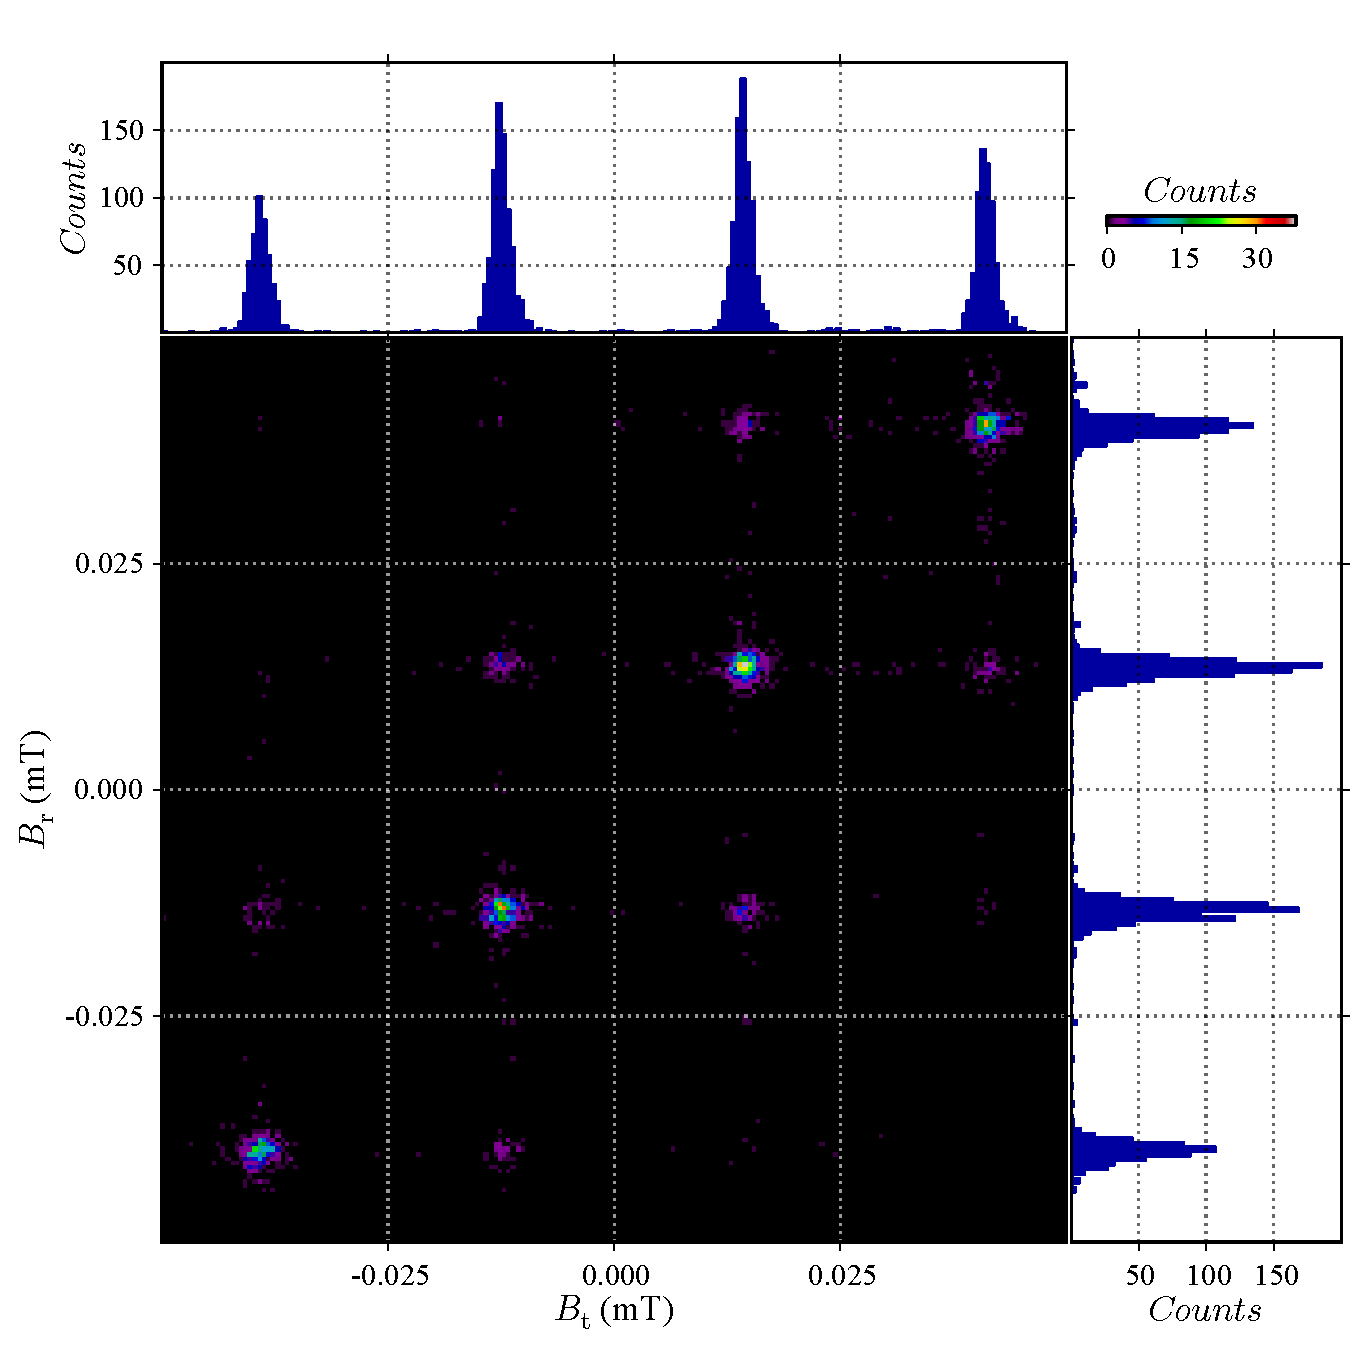
\includegraphics[scale=0.45]{Resultats/Chap2/Figure1/figure1.pdf} 
\caption{La cartographie couleur en deux dimensions représente l’histogramme de corrélation entre la position en champ magnétique des retournements ayant lieu durant la trace et la retrace.Celui-ci a été obtenu à partir de 22000 traces et retraces mesurées consécutivement et sans temps d'attente. Les histogramme à une dimension disposé le long des axes x et y représente respectivement les positions en champ magnétique des retournement durant la trace et la retrace. La prépondérance des éléments diagonaux atteste de la préservation de l'état de spin entre deux mesures.}
\label{correlations}
\end{figure}

L'évolution des états du spin nucléaire est représenté à l'aide d'un histogramme à deux dimensions. Le champ de retournement de la première mesure est repéré en abscisse et celui mesuré lors de la seconde mesure est représentée en ordonnée. Dans une telle représentation, les éléments diagonaux rendent compte d'un état de spin nucléaire qui ne change pas entre les deux mesures. Les éléments hors-diagonaux représente quant à eux las cas où l'état de spin nucléaire varie de $\Delta m_z^I = \pm 1,2,3$ où $m_z^I$ est la projection du moment angulaire du spin nucléaire sur l'axe $z$. La Fig.\ref{correlations} présente une telle mesure pour un temps d'attente nul. Pour faciliter la lecture, l'histogramme des champs de retournement de la première et deuxième mesures a été ajouté.

La Fig.\ref{evolution_temps} montre l'évolution de l'histogramme en fonction du temps d'attente entre les deux mesures. Les éléments diagonaux dominent jusqu'à un temps d'attente de $20$ secondes, prouvant que le spin nucléaire demeure majoritairement inchangé sur ce laps de temps. En revanche, pour un temps d'attente de $50$ secondes, on constate que les éléments diagonaux ne sont plus prépondérant signifiant le perte de l'état nucléaire entre les deux mesures. De plus, la résonance correspondant à l'état de spin $|-3/2 \rangle$ domine largement. Cela traduit la tendance du système à évoluer vers l'équilibre thermodynamique lorsque le temps d'attente devient trop élevé. Nus reviendrons sur ce dernier point dans la suite.

\begin{figure}[h]
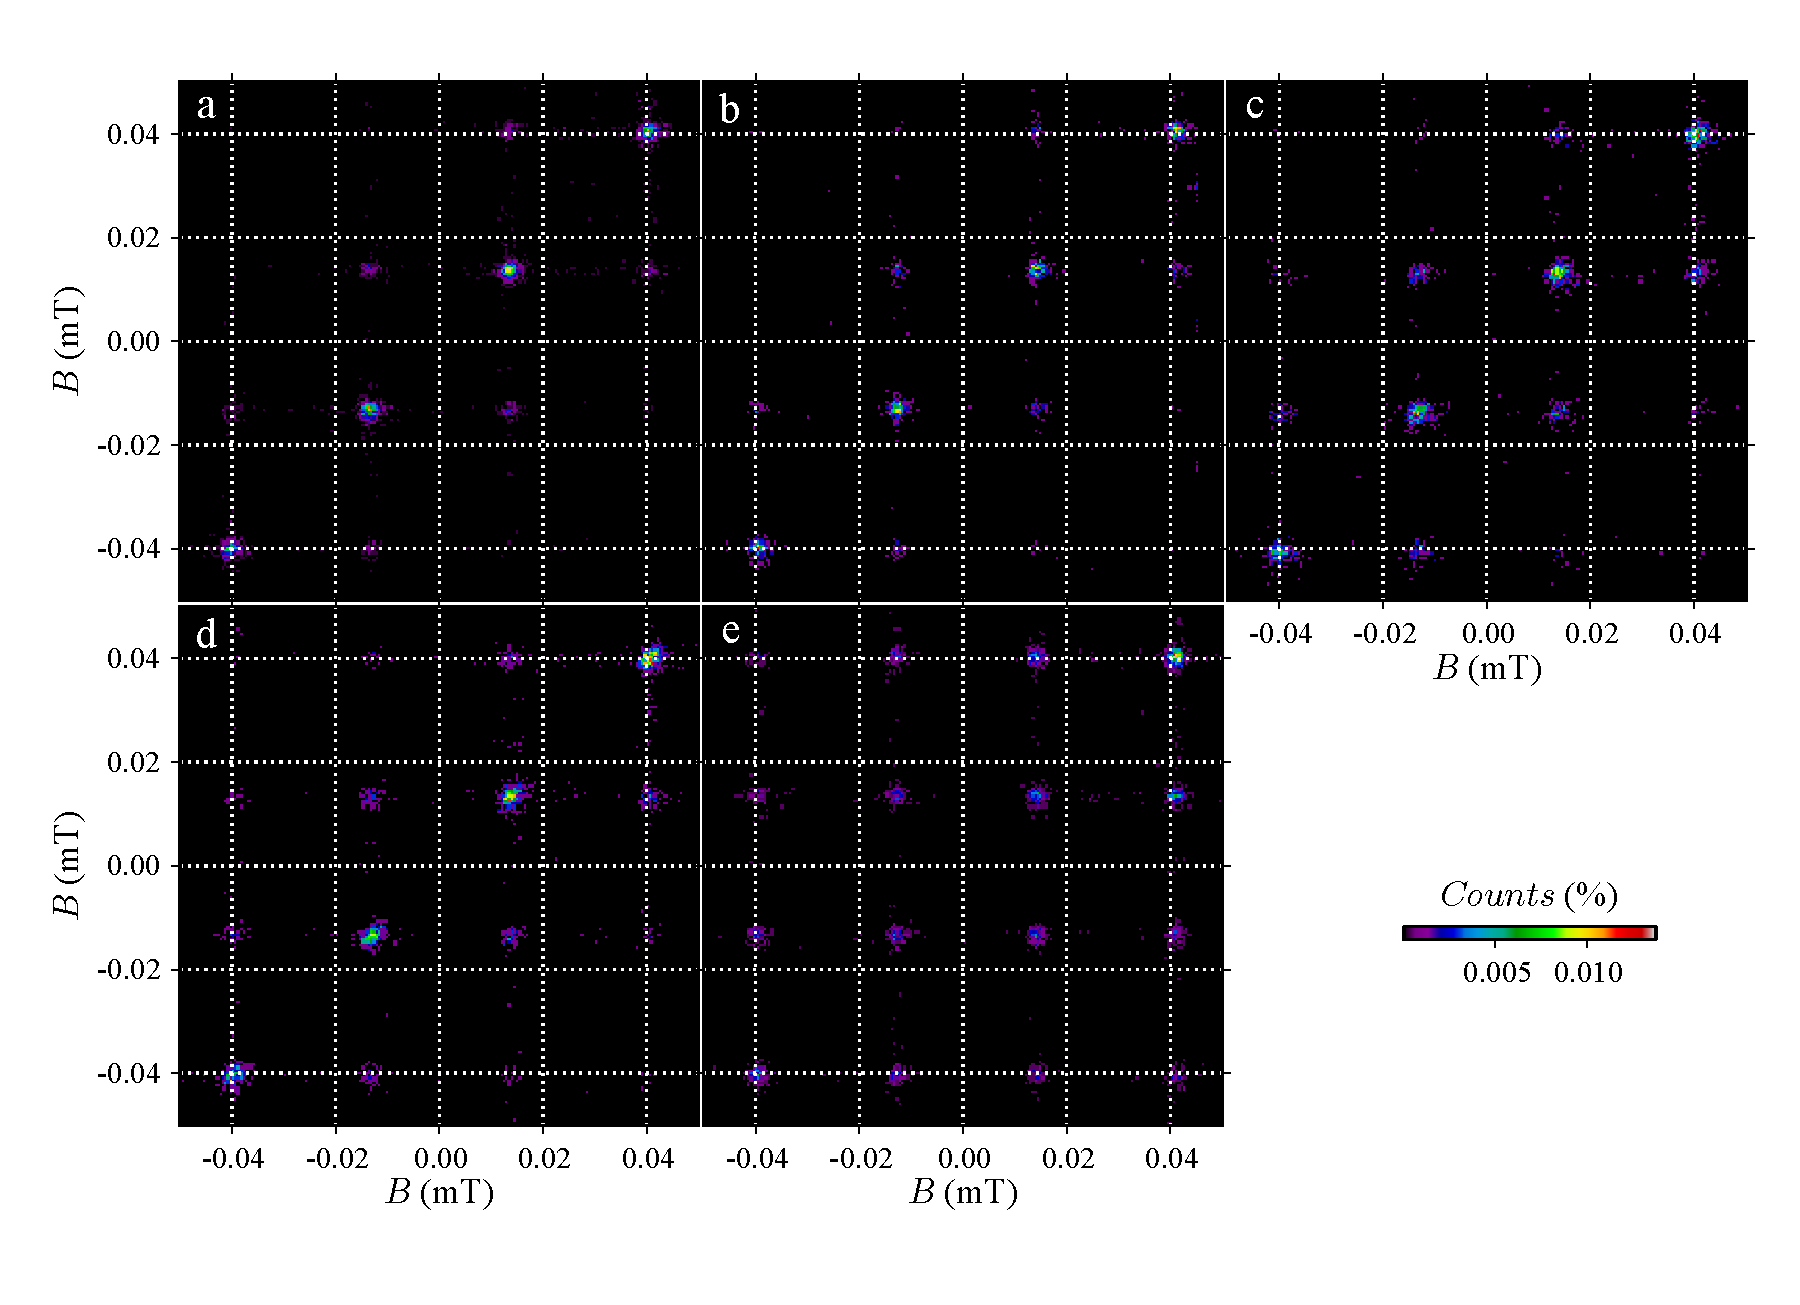
\includegraphics[scale=0.45]{Resultats/Chap2/Figure2/figure2.pdf} 
\caption{La cartographie a (b, c, d et e) présente un histogramme 2D rendant compte de la corrélation entre deux mesures obtenues durant la trace et la retrace, ces dernières étant séparé d'un temps d'attente de 0 secondes (5, 10, 20 et 50 secondes). La prédominance des élements diagonnaux pour des temps d'attente allant au-delà de la dizaine de seconde démontre le long temps de vie des états du spin nucléaire.}
\label{evolution_temps}
\end{figure}


\subsection{Perturbations induites par la mesure}
De m\^eme que nous pouvons étudier l'influence du temps d'attente sur le spin nucléaire, il peut \^etre intéressant d'évaluer l'influence de la mesure sur l'état de spin nucléaire. Pour cela, nous avons choisi d'utiliser la méthode présenté précédemment, en observant non plus l'évolution de l'état nucléaire en fonction du temps mais en fonction du nombre de mesures. Nous avons utilisé les donnée collecté sur 22000 balayages (11000 trace et autant de retrace) effectué sans temps d'attente.

La Fig.\ref{evolution_mesures} présente cette évolution après deux~(\textbf{a}), trois~(\textbf{b}), quatre~(\textbf{c}), cinq~(\textbf{d}) et six~(\textbf{e}) mesures. On constate qu'après 4 mesures, les éléments diagonaux domine toujours, pour ne commencer à s'atténuer qu'au bout de 6 mesures. Il est important de noté que chaque mesure est, en moyenne, séparée de 4 secondes, et donc, dans le cas de 6 mesures, cela correspond à un temps totale de plus de 20 secondes. Aux vues des résultats présentés dans la section précédente, on peut attribuer cette diminution de corrélation dans l'état du spin nucléaire au processus de relaxation interne au système, la procédure de mesure elle-même n'affectant qu'à la marge le système. 

La méthode de mesure de l'état de spin nucléaire par l'intermédiaire du QTM se révèle donc peu invasive, ce qui permet d'étudier les propriétés du système en négligeant son influence sur ce dernier.

\begin{figure}
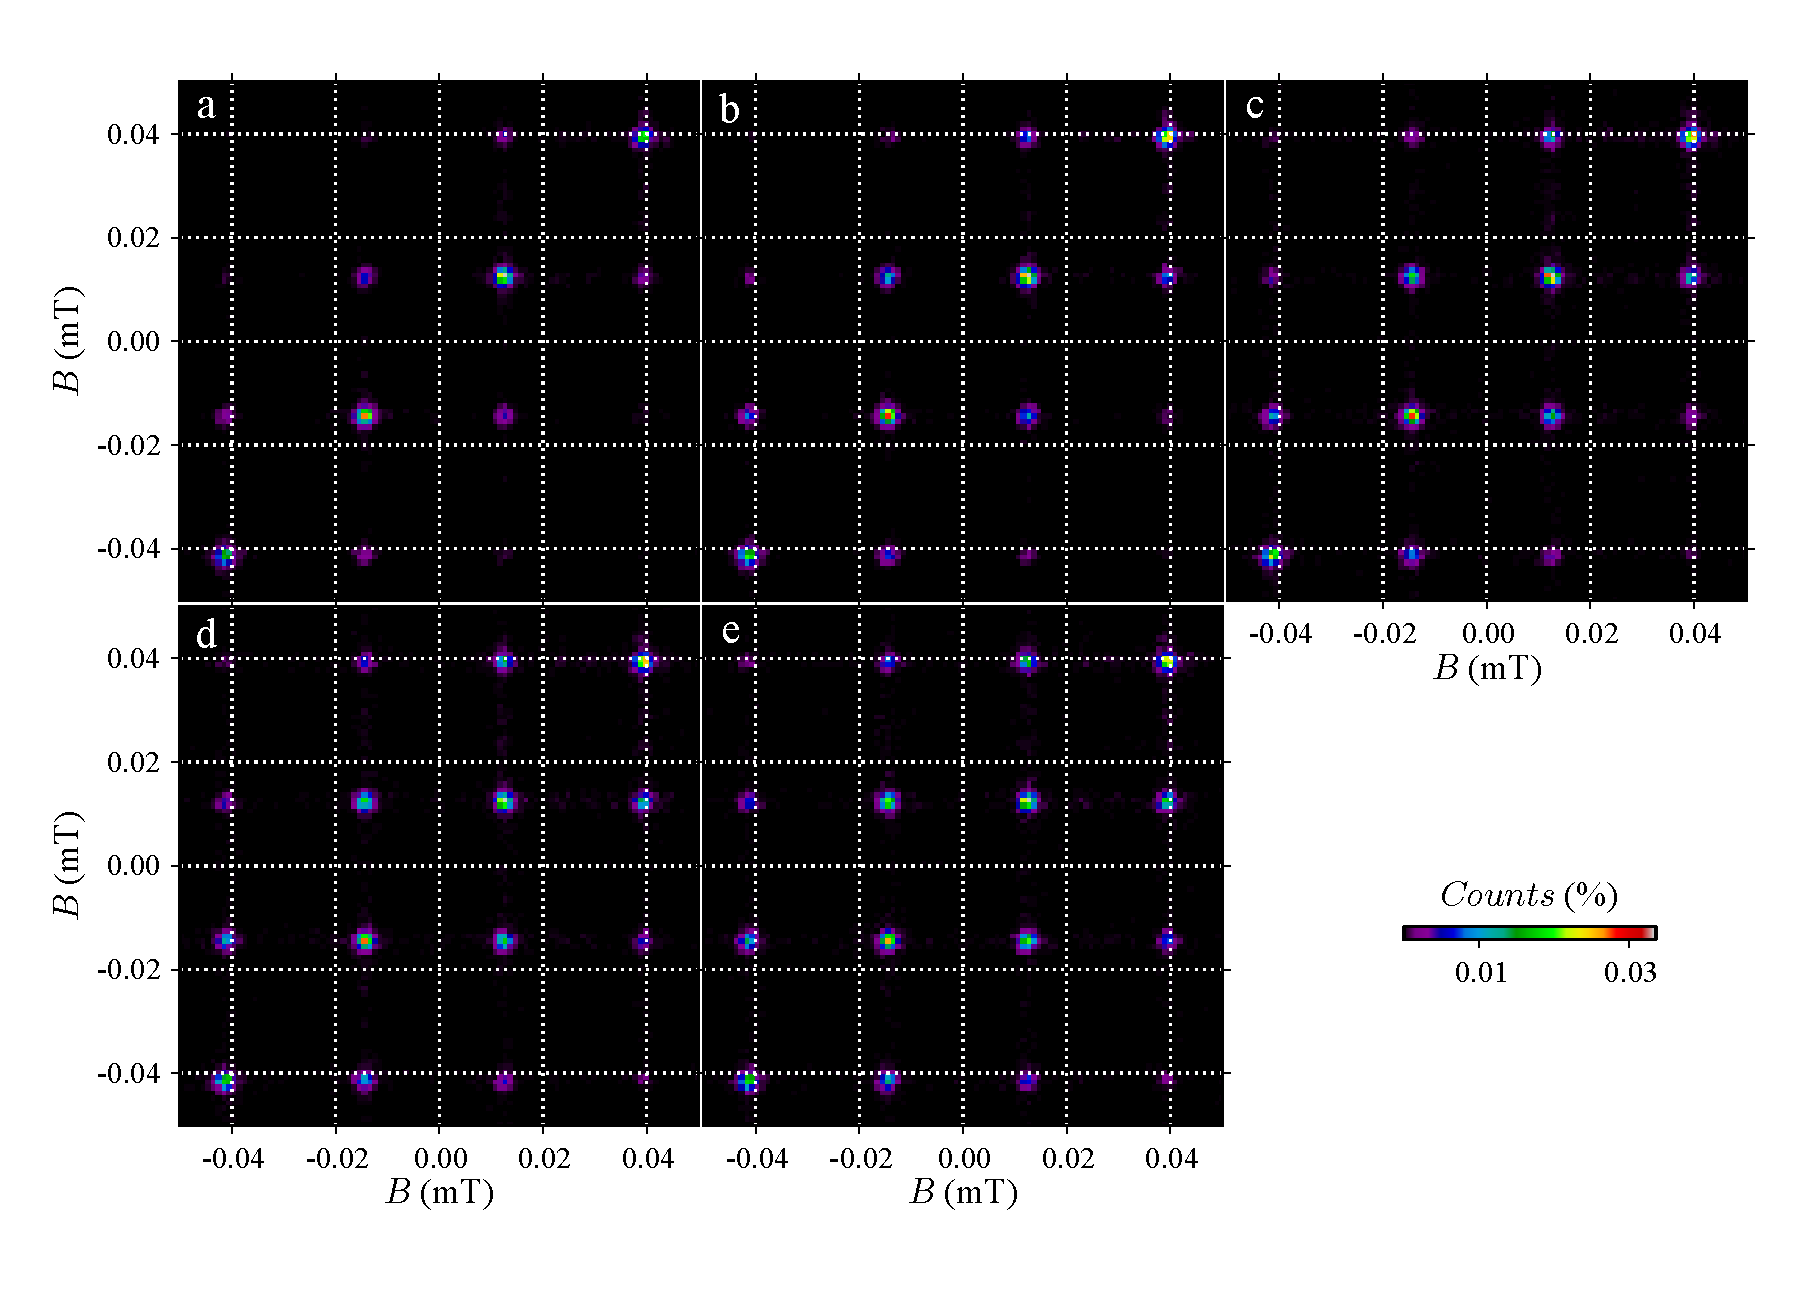
\includegraphics[scale=0.45]{Resultats/Chap2/Figure3/figure3.pdf} 
\caption{La cartographie a (b, c, d et e) présente un histogramme 2D rendant compte de la corrélation entre les états de spin nucléaire après deux (trois, quatre, cinq et six) mesures. On constate qu'après six mesures, les éléments diagonaux sont toujours dominant démontrant ainsi le faible influence de notre procédure de mesure sur l'état du spin nucléaire.}
\label{evolution_mesures}
\end{figure}


\subsection{Extraction de la population des états nucléaires}

Au chapitre précédent, nous avons montré qu'à travers un histogramme des positions en champ des renversements, on pouvait facilement identifier les différents états de spin.Nous allons utiliser cette m\^eme mesure en la présentant différemment. En effet, chaque retournement au voisinage d'une résonance peut \^etre attribuée à un état de spin précis, les différents résonances ne se recouvrant pas. En intégrant et en normalisant le nombre de mesures obtenues pour chaque état de spin nucléaire, on peut reconstruire leur distribution. C'est ce qui est présenté dans la Fig. \ref{extract_pop} ou l'histogramme original est montré en \textbf{a} et la population qui en est extraite en \textbf{b}.

Cependant, cette dernière contient en fait deux distributions, l'une relative à $J_z=-6$ et l'autre à $J_z=+6$ comme nous l'avons déjà montré. Il est cependant possible de les différencié à partir du signe du changement en conductance relatif à chaque mesure $\Delta g$. Dans la suite, du fait d'un initialisation à champ négatif, nous prendrons toujours pour référence la situation où $J_z=-6$ car il s'agit de l'état fondamental, donc plus probable, et il fournis donc une meilleure statistique.

\begin{figure}
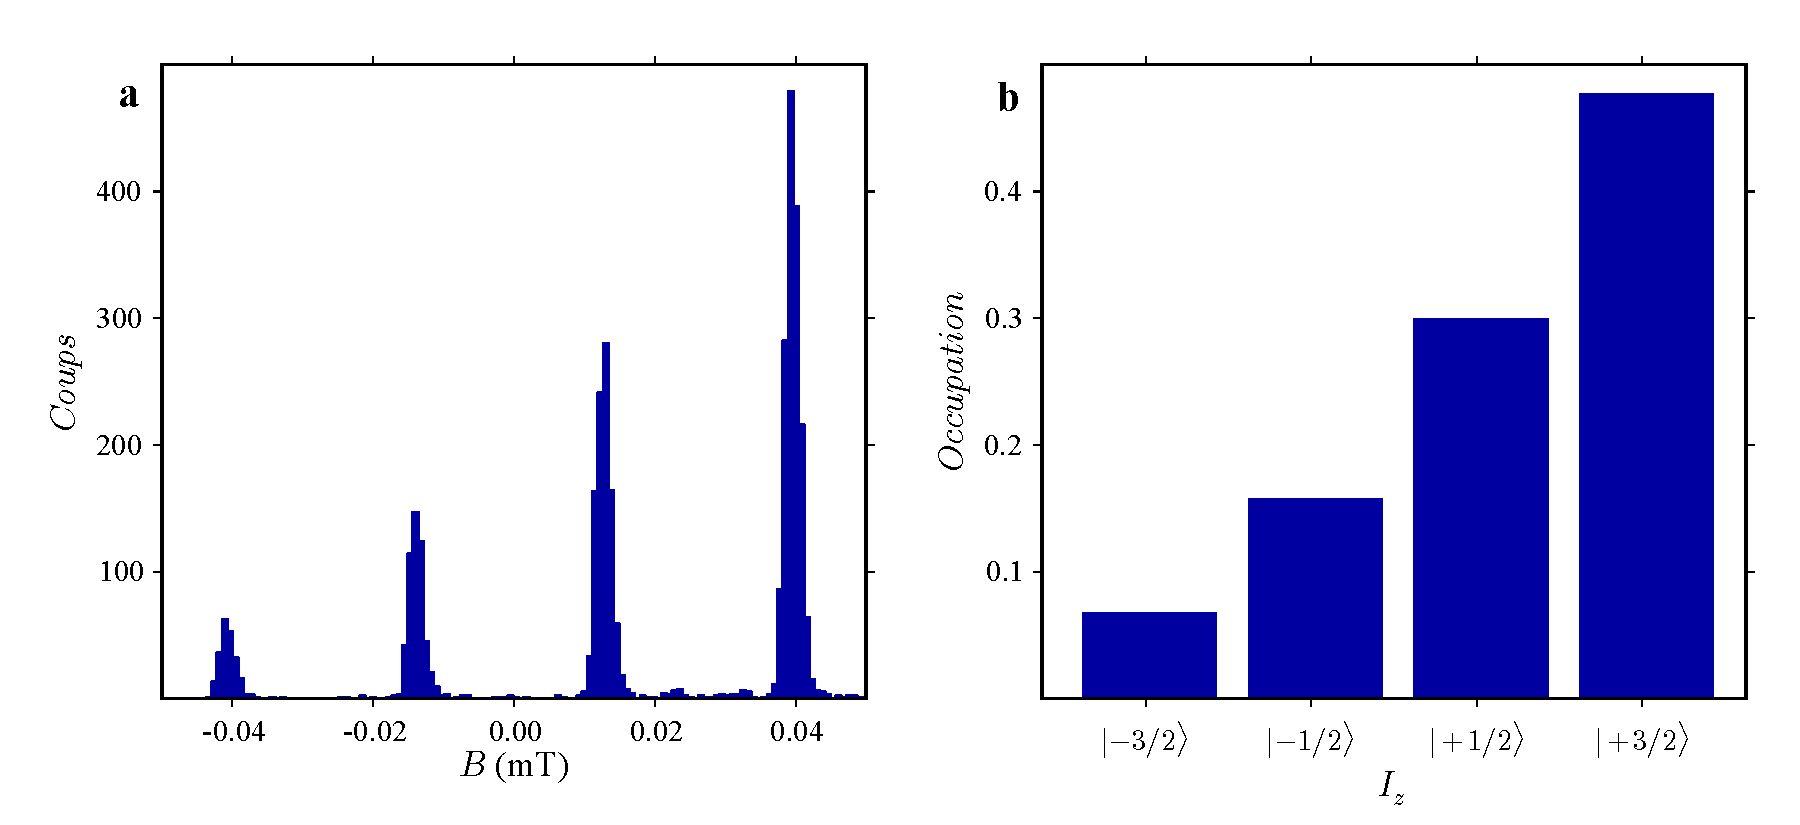
\includegraphics[scale=0.45]{Resultats/Chap2/Figure4/figure4.pdf} 
\caption{\textbf{a -} Histogramme des champs de retournement obtenue durant la trace et correspondant à la transition $J_z = +6 \rightarrow -6$. \textbf{b -} Population des états de spin nucléaire obtenue à partir de l'histogramme présenté en \textbf{a}. Du fait de la relaxation, on constate la prédominance de l'état fondamental $I_z=+3/2$ sur les autres états.}
\label{extract_pop}
\end{figure}

Nous allons maintenant utiliser cette technique d'extraction des populations pour étudier son évolution en fonction du temps pour deux environnements électrostatiques différents.

\subsection{Influence de la tension de grille sur la relaxation}
Afin d'évaluer l'influence de la tension de grille sur la relaxation, nous avons mesuré l'évolution de la population des états de spin en fonction du temps pour deux points polarisation ($V_g$,$V_{ds}$) différent : ($-0.9\, V$,$0\, V$) et ($-0.1\, V$,$0\, V$). Pour chacun de ces points nous avons fait varié le temps d'attente entre la retrace et la trace suivante de 0, 5, 10, 20 et 50 secondes et la population des états nucléaire a été reconstruite à partir des transitions obtenues durant la trace, en sélectionnant seulement celles correspondant à l'état fondamental $J_z=+6$.

La Fig.\ref{dynamique_spin}.\textbf{a} et \textbf{b} présentent les résultats obtenus. On constate immédiatement que les deux distribution évolue différemment. Pour la tension de grille $V_g = -0.9V$ la relaxation vers l'équilibre thermodynamique se fait plus lentement que lorsque $V_g = -0.1V$.  Ceci peut s'expliquer par la modification du courant circulant à travers le système du fait de la modification de la tension de grille. Celle-ci entraîne un changement dans les fluctuations de champ électrique  qui, en se couplant au moment quadripolaire du spin nucléaire, vont modifier les processus de relaxation.

Un analyse plus fine en grille n'a cependant pas permis déterminer le phénomène physique rendant compte de cette dépendance.

\begin{figure}
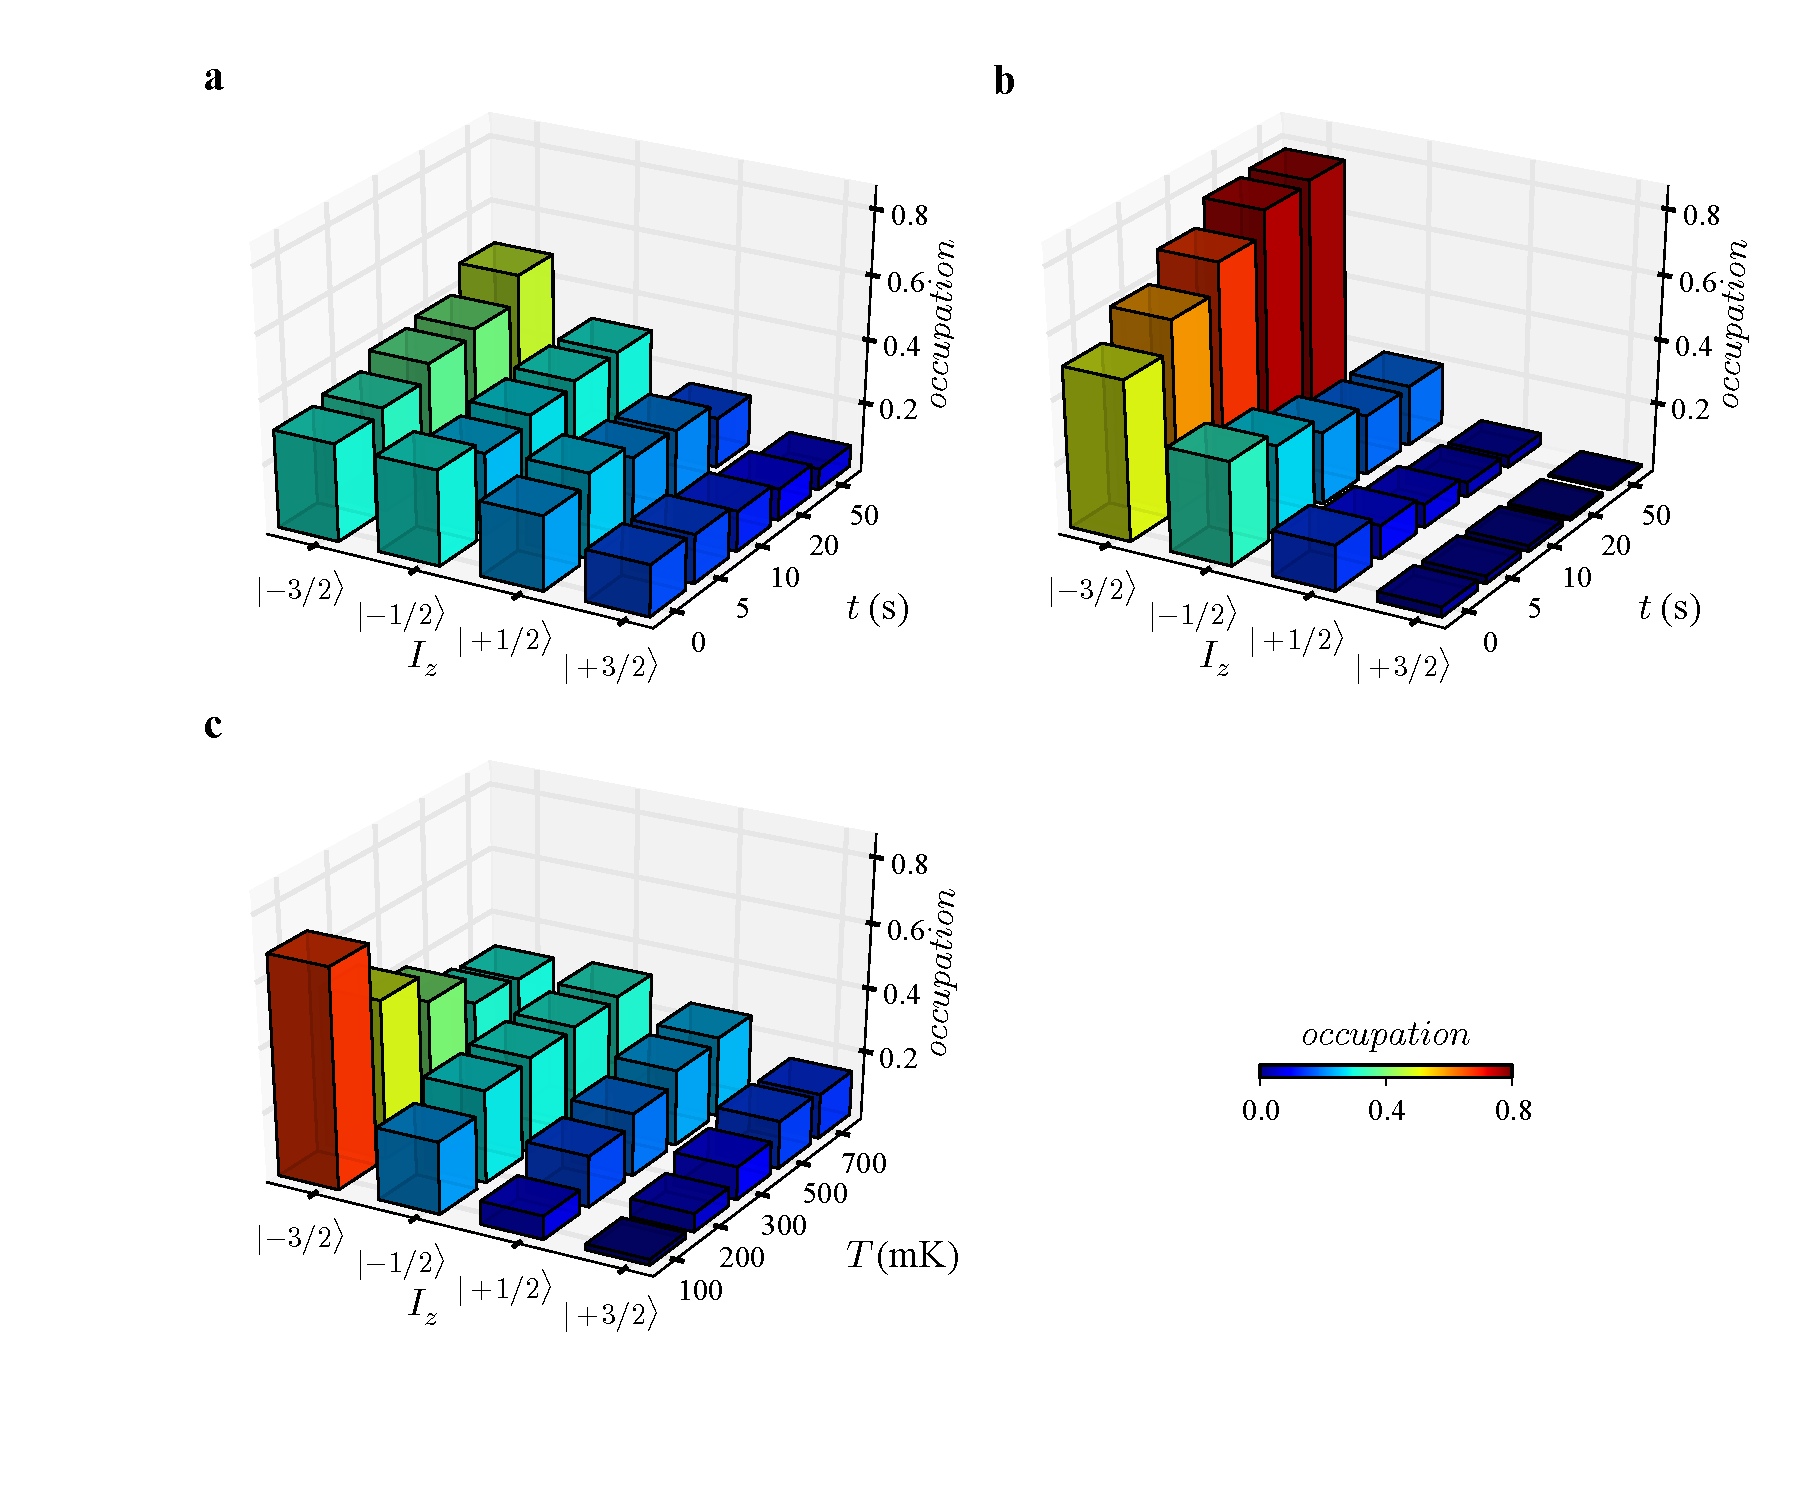
\includegraphics[scale=0.45]{Resultats/Chap2/Figure5/figure5.pdf} 
\caption{Evolution de la population des états nucléaire pour deux points de fonctionnement différent : \textbf{a}, $V_g = -0.9\,V$; et \textbf{b}, $V_g = -0.1\,V$ (avec à chaque fois $V_{ds} = 0\,V$. Ces deux mesures montrent clairement que le système évolue vers deux équilibres thermodynamique différent. \textbf{c}, dynamique du spin nucléaire pour un temps d'attente de 10 secondes, en fonction de la température $T$. Lorsque l'on augmente la température, la population des états de spin nucléaire évolue vers une occupation égale de tous les états.}
\label{dynamique_spin}
\end{figure}

\subsection{Influence de la température}

La température du spin nucléaire a également été mesuré. Pour cela, nous avons choisi de nous placer sur le second point de fonctionnement pour lequel l'équilibre est atteint plus rapidement, ce qui nous  a permis de choisir un temps d'attente relativement faible pour effectuer notre étude. En effet, au vu du nombre de mesures nécessaire (22000 mesures), on ne peut pas attendre le temps nécessaire à l'équilibre thermodynamique. Nous avons choisi un compromis en prenant un temps d'attente de 10 secondes. Bien attendu, comme le montre l'étude précédente, l'abscence d'équilibre ne nous permet pas de déduire, directement à partir de la distribution, la température du spin nucléaire.

Pour contourner cette limitation, nous avons choisi d'utiliser une méthode indirecte. Pour cela, la distribution des état nucléaire a été mesuré pour plusieurs température. La distribution observé pour $100\,mK$ a servie de référence, car celle-ci est très proche de la température électronique ($\sim 80\,mK$). La distribution ne va différé de la distribution de référence qu'à condition que la température imposé au système soit supérieur à la température nucléaire de référence obtenue à $100\,mK$.

La Fig.\ref{dynamique_spin}.\textbf{c} présente l'évolution de la distribution à $10\,$ seconde en fonction de la température. La distribution évolue entre 100 et 200$\,mK$ et celle-ci est largement modifié pour $T\geq 300mK$. Les états de plus hautes énergies commencent à se peupler pour tendre vers l'équiprobabilité vers $T=700\,mK$. On peut donc en déduire qu'à la température de base, la température d'équilibre du spin nucléaire se situe entre 100 et 200 $\,mK$, preuve que le spin nucléaire peut être refroidi de manière efficace. En effet, cette température d'équilibre est très proche de la température électronique de notre système évalué autour de $100\,mK$.


=======

\mainmatter 

%\chapter{Spintronique moléculaire}

\section{Spintronique et Électronique moléculaire}
La micro-électronique a su évoluer au gré des développements scientifiques. Elle, a tout d'abord, su tirer avantage des travaux sur la magnéto-résistance géante au travers d'une nouvelle discipline : la spintronique. Pendant presque deux décennies, celle-ci a permis d'améliorer, de plusieurs ordres grandeurs, les capacités de stockage des composants électroniques. Plus récemment, le développement de molécules organiques semi-conductrices~\cite{Tsumura1986,Horowitz1990,Lin1997} a poussé, encore une fois, l'électronique dans une nouvelle voie : celle de l'électronique organique.

\subsection{La spintronique}
La spintronique est une branche de l'électronique où, en plus de la charge, le degré de liberté du spin de l'électron est utilisé. Elle est notamment à l'origine des avancés technologiques les plus récentes, telles que la MRAM~(Magnetic Random Access Memory), ou bien encore, les têtes de lecture des disques durs~(cf Fig.\ref{SpinValve}.\textbf{b}). Mais le dispositif le plus célèbre, à la base des technologies précédemment citées, reste sans doute la vanne de spin. Celui-ci permet de filtrer les électrons en fonction de l'orientation de leur spin (soit \textit{up}, soit \textit{down}), autorisant un couplage direct entre magnétisme et courant électrique. La découverte du phénomène de magnétorésistance géante~(cf Fig.\ref{SpinValve}.\textbf{a}), à l'origine de ce filtrage, a d'ailleurs value à ses découvreurs, Albert Fert~\cite{Baibich1988} et Peter Grünberg~\cite{Gruenberg1986}, le prix Nobel de Physique en 2007.

\begin{figure}
\centering 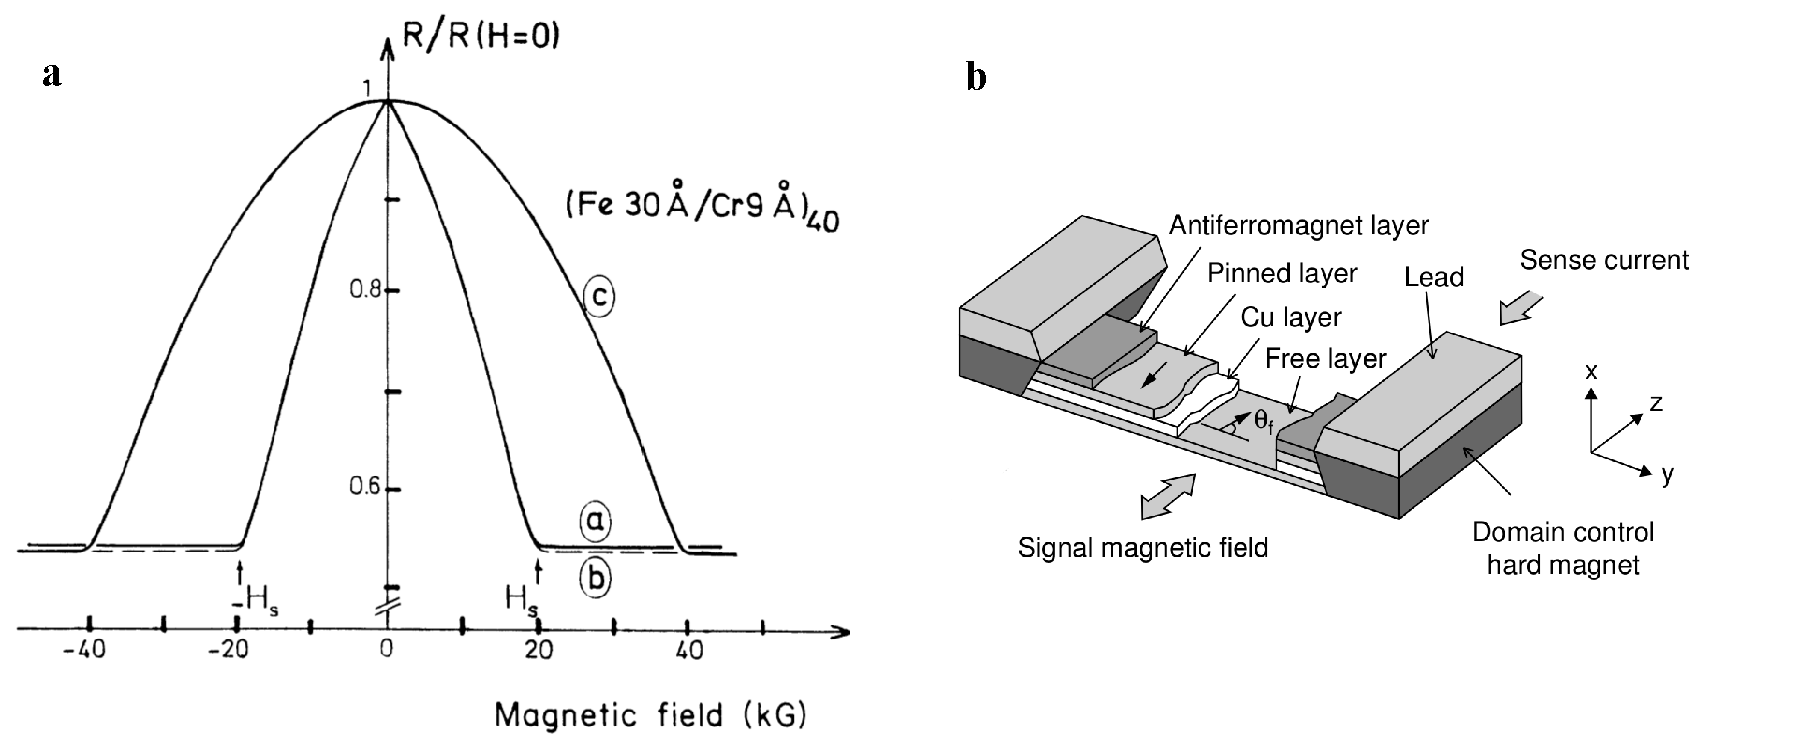
\includegraphics[scale=0.45]{Spintronique/SpinValve/SpinValve.pdf}
\caption{\textbf{a} : mesure de la résistance d'une vanne de spin mettant en évidence la magnéto-résistance géante~(extrait de ~\cite{Baibich1988}).  \textbf{b} : Schéma d'une tête de lecture de disque dur, dont le fonctionnement est basé sur le phénomène de magnéto-résistance~(extrait de~\cite{Hitoshi2001}).}
\label{SpinValve}
\end{figure}



La spintronique, dans ses applications, reste cependant cantonnée au stockage de  l'information~\cite{Awschalom2007}. Des propositions de transistors de spin, directement commandés par le spin électronique, ont pourtant été faites~\cite{Datta1990}, et certains dispositifs ont également été réalisés~\cite{Johnson1996,Huang2007}. Mais de tels systèmes n'ont pas, pour l'instant, quitté les laboratoires.

De plus, elle se heurte aux défis de la miniaturisation, qui ne lui sont pas spécifiques, mais qui se posent à l'ensemble de l'électronique. Le salut des futurs dispositifs pourrait bien se trouver dans l'électronique organique.

\subsection{L'électronique organique}
Devant le besoin toujours plus grand de miniaturisation des dispositifs, les chercheurs et les industriels se sont vite rendu compte des limites des techniques de fabrication traditionnelles. Elles consistent à graver, au sein d'un matériau massif, les structures nanométriques nécessaires à la production de l'électronique actuelle. C'est l'approche dite``\textit{Top-Down}"

Devant les progrès récents de la chimie organique, une seconde solution est apparue, faisant appel à cette dernière  pour produire les objets de petite taille, et les disposer de manière contrôlée : c'est l'approche dite ``\textit{Bottom-Up}". Dans cette approche, deux caractéristiques des molécules sont exploitées : leur capacité à s'auto-assembler, c'est à dire à adopter une configuration précise, ``programmée" à travers les ligands; la possibilité de fabriquer des milliards de molécules toutes identiques, avec une grande pureté. 

L'histoire de l'électronique moléculaire est cependant relativement récente. Comme le rappelle G. Horowitz dans~\cite{Klauk2007}, l'industrie s'est finalement intéressée à ce domaine de l'électronique, lorsque les semi-conducteurs organiques sont devenus plus performants, en terme de mobilité électronique, que le silicium amorphe~\cite{Lin1997}.
\begin{figure}
\centering 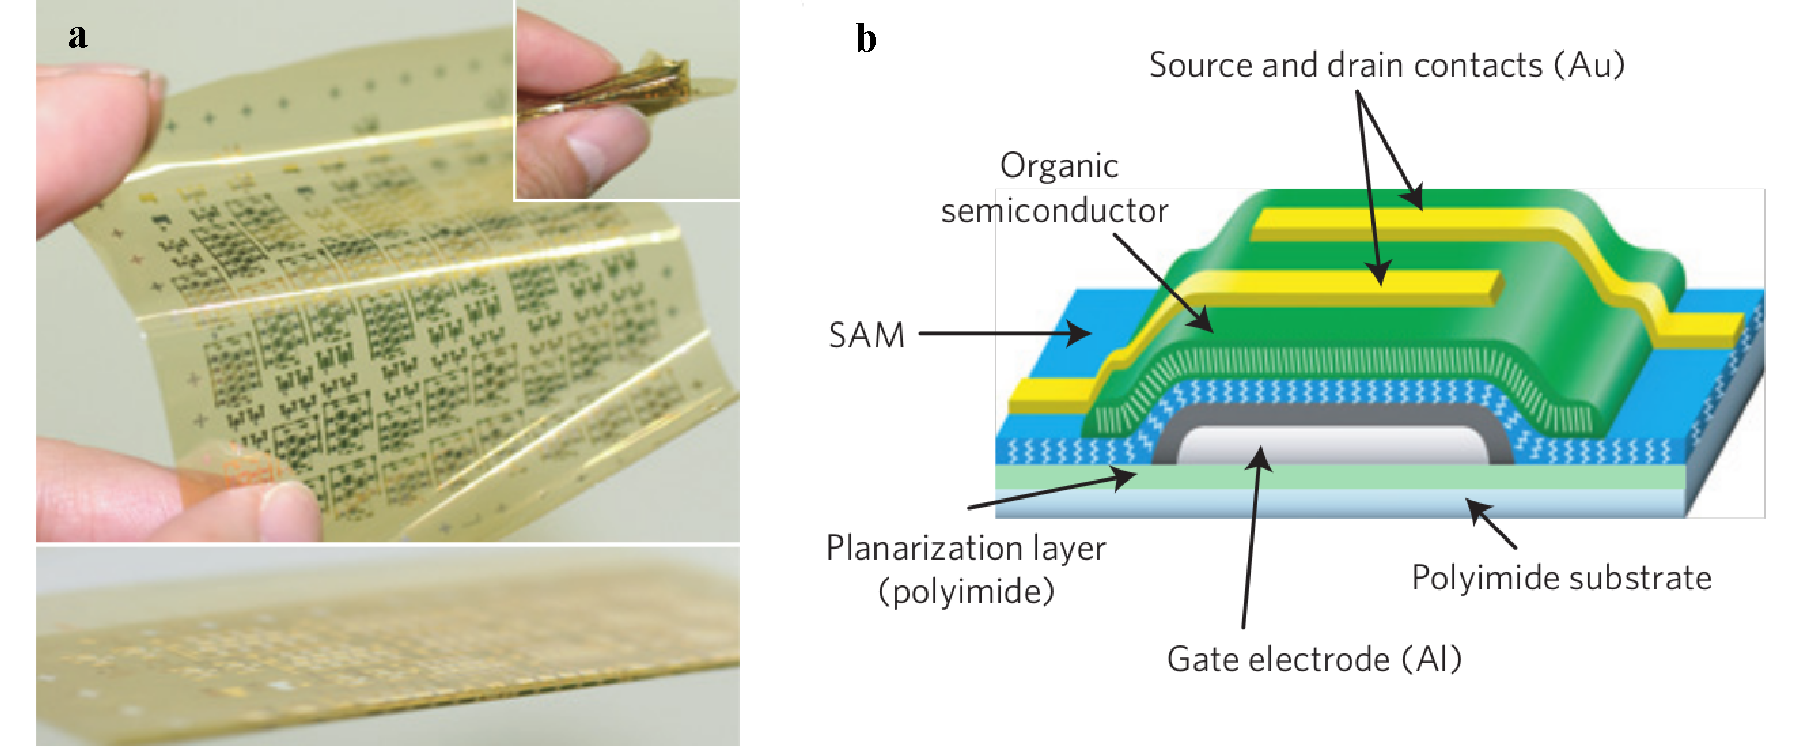
\includegraphics[scale=0.45]{Spintronique/MolecularElec/MolecularElec.pdf}
\caption{\textbf{a} : Photographie d'un substrat de polymide contenant des transistors organiques. \textbf{b} : Vue en coupe d'un transistor organique~(figure extraite de~\cite{Sekitani2010}).}
\label{MolecularElec}
\end{figure}


Depuis, de nombreux dispositifs issus de l'électronique moléculaire ont vu le jour, comme les  transistors à base de films fins organiques (ou OFTFs - cf Fig.\ref{MolecularElec}). Mais aucune application n'a, à ce jour, tiré partie de la taille nanométrique des molécules, et la route est encore longue avant l'obtention de dispositifs commerciaux, ne mettant en jeux que quelques molécules, voire une seule.

Comme le souligne les auteurs de~\cite{Gatteschi2006} , une conséquence plus inattendue du développement de l'électronique moléculaire, est d'avoir participé à l'essor du magnétisme moléculaire, domaine que nous allons aborder maintenant.


\section{Le magnétisme moléculaire}
L’intérêt réciproque entre l'électronique organique et le magnétisme moléculaire, réside dans le fait que les aimants moléculaires sont de très bons candidats pour la réalisation de dispositifs de spintronique~\cite{Bogani2008,Sanvito2011}.

\begin{figure}
\centering 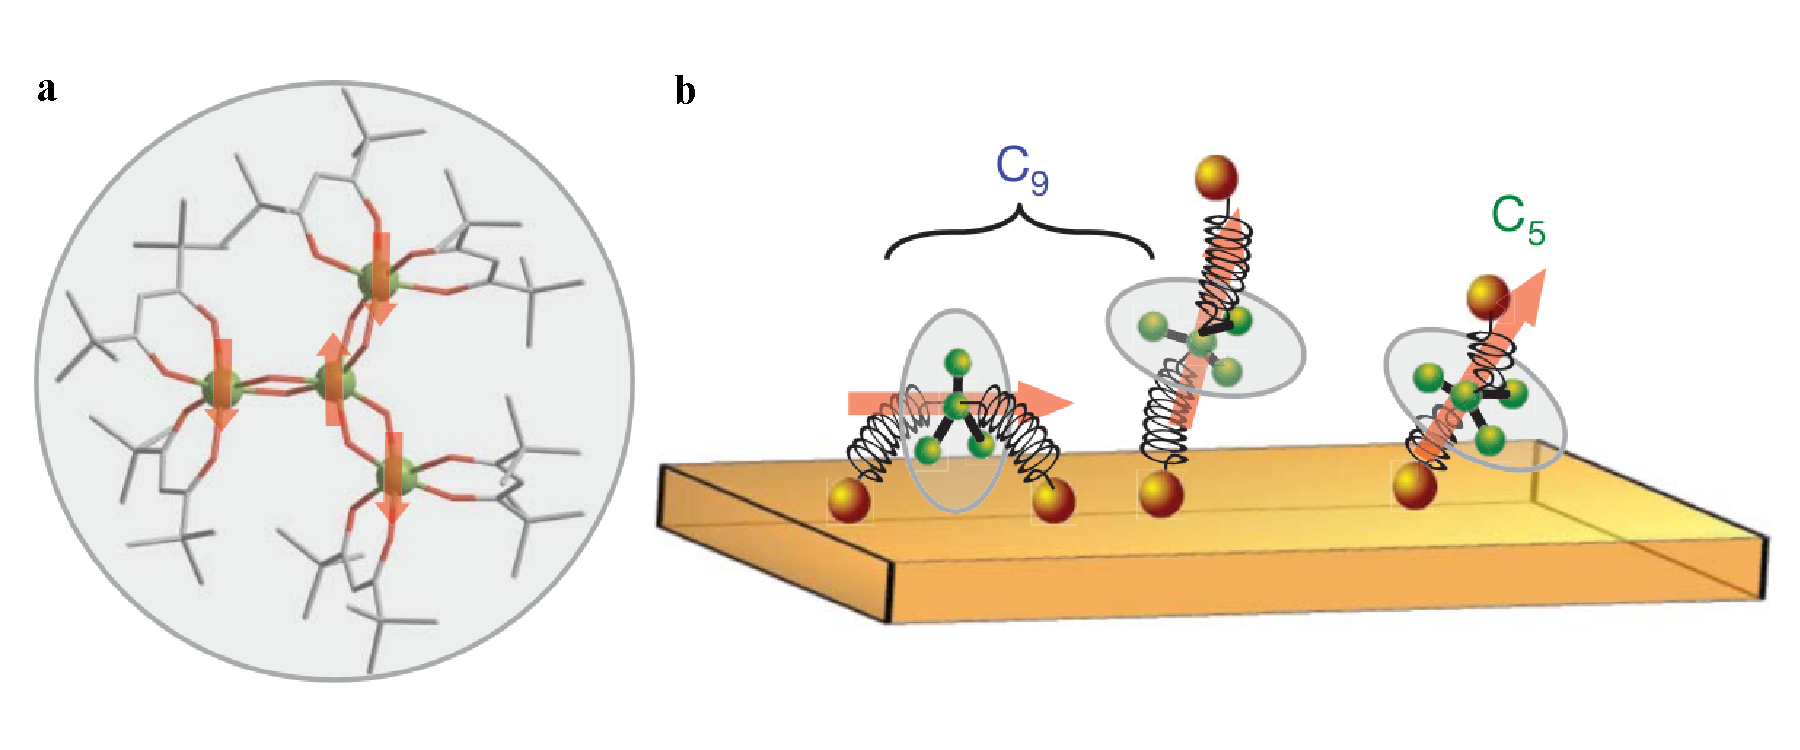
\includegraphics[scale=0.45]{Spintronique/MolecularMag2/MolecularMag2.pdf}
\caption{\textbf{a} : Structure du \textit{cluster} de Fe$_4$. \textbf{b} : Représentation des différent mode d'ancrage, correspondant à différentes orientations de l'axe facile~(extrait de~\cite{Mannini2010}).}
\label{MolecularMag2}
\end{figure}

La première raison, déjà évoquée, est la possibilité qu'ils offrent d'implémenter une approche ``Bottom-Up".
Notamment, par l'ajout de ligand, les molécules peuvent s'auto-assembler pour former des structures parfois complexes, sans la mise en œuvre de techniques lithographiques conventionnelles. Par exemple, l'équipe de Roberta Sessoli a récemment montré, qu'il était possible de contrôler la direction préférentielle de l'aimantation adoptée par les SMMs, une fois ces deniers déposés sur une surface d'or, par le choix de ligands adaptés. A l'aide du système obtenu, elle a également mis en évidence le retournement de l'aimantation de la molécule de Fe$_{4}$~\cite{Mannini2010}~(cf Fig.\ref{MolecularMag2}).

Par ailleurs, les aimant moléculaires, de par leur taille, représentent la solution de stockage ultime. L'information pourrait être coder par l'orientation de leur moment magnétique, extrêmement stable à basse température, accroissant ainsi la capacité de stockage informatique.

En outre, il est possible de rendre leur magnétisme, dépendant de stimulus extérieurs tels que la lumière, ou bien encore la chaleur. De telles propriétés pourraient \^etre mises en oeuvre dans la fabrication de détecteurs, de mémoires, ou bien encore, dans la conception de dispositifs opto-électroniques~\cite{Sanvito2011}.

Cependant, l'électronique conventionnelle n'est pas la seule possibilité d'application. En effet, le magnétisme moléculaire est régie par les lois de la mécanique quantique. A ce titre, ils pourraient \^etre utilisés pour implémenter les fameux bits quantiques, ou qbits, dans le cadre de l'information quantique. C'est notamment à l'investigation de ces propriétés quantiques que se consacre l'étude du magnétisme moléculaire.
 
Essayer de dresser un panel complet du magnétisme moléculaire est un travail complexe, auquel je ne m'attacherai pas ici. Pour cela, je renvois le lecteur à~\cite{Gatteschi2006} et son excellente introduction. Je ne vais souligner ici que quelques étapes présentant certains des phénomènes physiques majeurs mis en évidence dans les aimants moléculaires.

La première mesure d'un effet quantique sur un aimant moléculaire~(SMM ou Single Molecular Magnet) a été obtenue en 1995 à partir d'un échantillon de poudre d'une molécule maintenant bien connue : le Mn$_{12}$Ac~\cite{Friedman1996}. Quelques temps plus tard, cette mesure était confirmée à l'aide d'un cristal moléculaire de Mn$_{12}$Ac~\cite{Thomas1996}. Ce phénomène quantique est connu sous le nom de retournement de l'aimantation par effet tunnel~(ou QTM - Quantum Tunneling of the Magnetization).
Celui-ci correspond au retournement de l'aimantation d'une molécule malgré la présence d'une barrière de potentiel entre les deux orientations opposées~(cf Fig.\ref{MolecularMag}.\textbf{a}). Ceci n'est possible que lorsque deux états du système, situés de part et d'autre du puits de potentiel, sont amenés en résonance à l'aide d'un champ magnétique. Le phénomène de QTM ne peut se faire que pour des valeurs de champ magnétique bien précises, donnant lieux à des mesures de cycles d'hystérésis présentant des marches~(cf Fig.\ref{MolecularMag}.\textbf{b}).

\begin{figure}
\centering 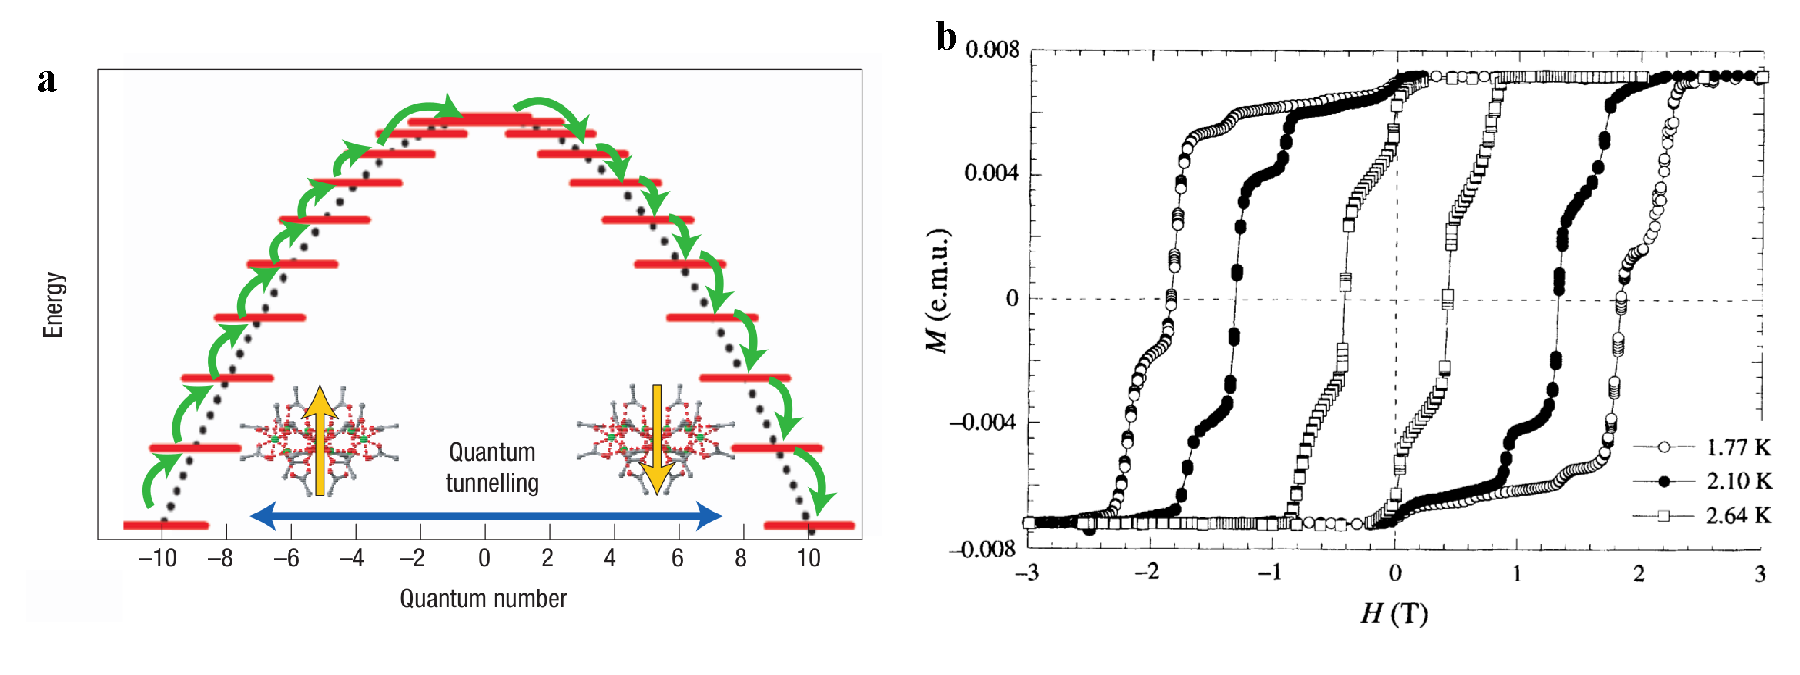
\includegraphics[scale=0.45]{Spintronique/MolecularMag/MolecularMag.pdf}
\caption{ \textbf{a} : échelle des énergies des différents états de spin pour un spin $S=10$. Le renversement peut s'effectuer par effet tunnel~(QTM - Quantum Tunneling of the Magnetizion) lorsque un des niveaux dans le premier puit est en résonance avec un niveau dans le second~(flèche bleu). L'aimantation peut également ``monter" l'échelle des énergies par l'absorbtion de phonon, pour ensuite redescendre dans le second puits en émettant des phonons~(flèche verte)~(extrait de~\cite{Bogani2008}).\textbf{b} : Première mesure du phénomène de QTM sur un cristal moléculaire de Mn$_{12}$Ac, mettant en évidence la structure en marche associée au retournement par effet tunnel~(extrait de~\cite{Thomas1996}).}
\label{MolecularMag}
\end{figure}

Trois ans plus tard, Wolfgang Wernsdorfer et Roberta Sessoli mettaient en évidence une oscillation dans les probabilités de retournement par QTM, dû à un effet quantique d'interférence semblable à la phase de Berry~\cite{Wernsdorfer1999}. Dans ce phénomène, les interférences se font entre le différents ``chemins" que l’aimantation peut prendre sur la sphère de Bloch lors de son renversement. Ceci se traduit par une variation dans les probabilités de retournement, et donc, par une modulation de la hauteur des marches associés au QTM.

Mais l'étude du magnétisme moléculaire ne s'arr\^ete pas au moment magnétique électronique. Il peut également mettre en jeu le magnétisme nucléaire au travers du couplage hyperfin. Ceci rend les aimants moléculaires possédant des propriétés liées au spin nucléaire très attractifs, d'autant que de nombreuses études présentent ce dernier, comme un qbit idéal dans le cadre de l'information quantique. C'est ainsi que la structure hyperfine de certains terres rares a pu être explorée. En effet, la position en champ des retournements par QTM peut être, dans certains cas, fortement influencée par l'état du spin nucléaire. Le TbPc$_{2}$ a notamment été caractérisé en détail à l'aide de la technique micro-SQUID, et les paramètres du couplage hyperfin ont pu être extraits de la mesure de l'aimantation d'un cristal moléculaire~\cite{Ishikawa2005}. D'autres noyaux de terres rares ont également été analysés avec succès, à l'aide d'une structure moléculaire identique~\cite{Ishikawa2005a}.

Les implications de ses travaux dans le domaine de l'électronique organique, n'ont pas laissé la communauté du magnétisme indifférente, et la question de l'interaction entre aimant moléculaire et surface métallique s'est rapidement posée. Une étude portant sur une molécule de Mn$_{12}$ déposée sur une surface d'or a été réalisée en 2008~\cite{Mannini2008} en combinant différents moyens d'analyse~(XAS et XMCD). Elle conclue que la structure de l'aimant moléculaire est modifiée lorsque ce dernier est déposé sur une surface, et que le magnétisme est également affecté. Cette fragilité a été confirmée par une seconde étude~\cite{Mannini2009}, soulignant l'importance du choix du SMM pour les applications de spintronique moléculaire.

Toutefois, une meilleure compréhension du magnétisme moléculaire et de ses interactions avec l’environnement, passe par le développement de la spintronique moléculaire, seul moyen d'investigation à l'échelle de la molécule unique. C'est donc également dans cette voie que se sont engagés à la fois les chimistes et les physiciens.


\section{La spintronique moléculaire}
La spintronique moléculaire a pour but de combiner les techniques de la spintronique avec les nouveaux développements de l'électronique moléculaire et de la chimie, afin de produire de nouveaux dispositifs. Ces derniers seraient susceptibles de compléter, ou éventuellement, remplacer les technologies tout semi-conducteur déjà existantes. Cette discipline a connu une évolution rapide ces dernières années, bénéficiant des dernières avancés en matière de lithographie, mais aussi de la mise en synergie du travail des physiciens et des chimistes. 

Dans ce paragraphe, je ne présenterai bien sûr qu'une petite partie des nombreux travaux effectués dans le domaine. Ceci ne constitue, en aucun cas, une liste exhaustive des expériences réalisées, ni m\^eme une sélection des travaux les plus importants. Elle permettra au lecteur, je l'espère, de situer nos recherches par rapport à celles en cours dans d'autres laboratoires. De plus, je me limiterai ici aux dispositifs ne comportant qu'un nombre limité de molécules, de l'ordre de l'unité, généralement utilisés dans les laboratoires de recherche fondamentale.
\subsection{État de l'art}

\subsubsection*{Du premier transistor moléculaire...}
La première expérience de mesure de courant à travers une molécule unique a été réalisée en 1995 à l'aide d'un microscope à effet tunnel~\cite{Joachim1995}~(ou STM). Il s'agissait de mesurer la résistance à travers une molécule de C$_{60}$ déposée sur une surface d'or. Il n'était pas question d'obtenir un transistor, puisque seul deux terminaux étaient présents à savoir, la surface conductrice et la pointe du STM~(cf Fig.\ref{MolSpintro2}.\textbf{d}).

Cette expérience, et celles qui ont suivi, ont encouragé le développement de nouvelles techniques, permettant de piéger une molécule unique dans un dispositif de mesure. C'est ainsi qu'est apparu la technique dite de ``break junction"~\cite{Zhou1995}. Elle consiste à suspendre un fin pont métallique déposé sur un substrat flexible, puis à plier le support jusqu'à obtenir une cassure~(cf Fig.\ref{MolSpintro2}.\textbf{c}). La taille de celle-ci peut être ensuite modulée en faisant varier la courbure imposée à l'échantillon. A l'aide de ce dispositif, Reed \textit{et al.} ont pu mesurer, en 1997, des molécules de benzene-1,4-dithiol et étudier l'influence du couplage entre les électrodes et la molécule, sur la conductance mesurée~\cite{Reed1997}. Cette technique présente cependant l'inconvénient de ne pas pouvoir disposer d'une grille locale permettant de moduler le potentiel de la molécule.

\begin{figure}
\centering 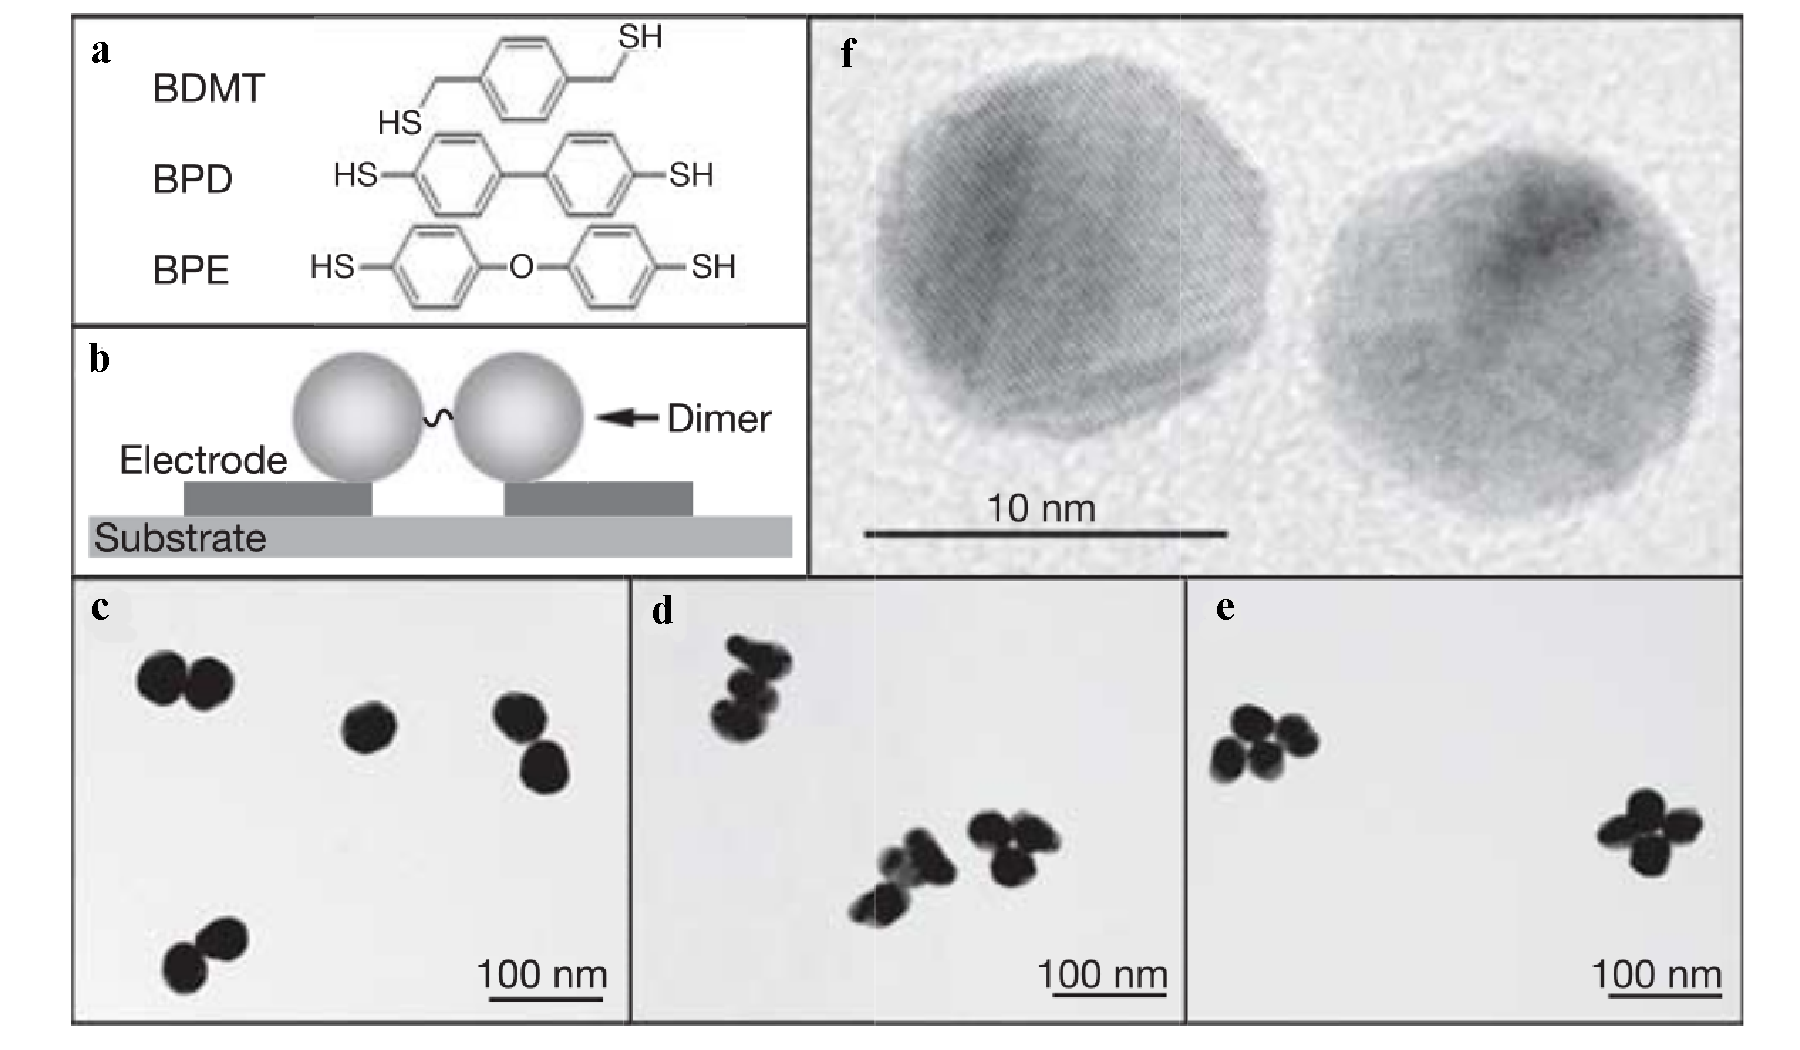
\includegraphics[scale=0.45]{Spintronique/MolSpintro2/MolSpintro2.pdf}
\caption{\textbf{a} : image obtenue par microscopie électronique à balayage d'une jonction moléculaire obtenue par technique d'électromigration, ainsi que la vue d'artiste correspondante~(extrait du site WEB de l'université de Tel Aviv). \textbf{b} : image par microscopie électronique à transmission~(TEM) d'un dimer, à base de BDMT~(1,4-
benzenedimethanethiol), constitué par deux billes d'or de $10\,nm$. Le nanomètre qui sépare les deux billes correspond approximativement à la taille de la molécule de BDMT~($0.9\,nm$).(Figure extraite de~\cite{Dadosh2005}). \textbf{c} : image par microscopie électronique à balayage d'une jonction à cassure~(image CEA/LEM). \textbf{d} : image d'artiste d'une mesure STM~(extrait de \cite{Leary2011}).}
\label{MolSpintro2}
\end{figure}


Pour pallier à cet inconvénient, il a fallu attendre encore 3 ans et la réalisation du premier transistor à molécule unique~\cite{Park2000}. Celui-ci consistait en un atome de C$_{60}$ piégé entre deux électrodes d'or déposées sur une grille. Ce dispositif a été obtenu en utilisant un phénomène bien connu des micro-électronicien, puisqu'à l'origine de nombreuses défaillances dans les dispositifs électroniques~\cite{Ho1989,Tu1992} : l'électromigration~(cf Fig.\ref{MolSpintro2}.\textbf{a}). Nous présenterons cette dernière en détail dans le chapitre consacré à la fabrication de notre échantillon. 
L'expérience menée sur ce premier transistor moléculaire, avait mis en évidence le couplage entre les modes de vibrations moléculaires et les caractéristiques de transport électronique. De plus, la grille se révélait suffisamment efficace pour modifier l'état de charge de la molécule de C$_{60}$, permettant d'obtenir les premiers diamants de Coulomb associés à une molécule unique.

Une étape supplémentaire a été franchie par le groupe de A. Yacoby~\cite{Dadosh2005}~(cf Fig.\ref{MolSpintro2}.\textbf{b}) Ils ont mis au point la première approche réellement ``Bottom-Up" en attachant chimiquement une molécule à deux billes d'or de quelques nanomètres, pour venir ensuite contacter ces dernières à l'aide de deux électrodes. \`A ma connaissance, cette technique n'a été réutilisée qu'une seule fois depuis~\cite{Jain2009}. Elle illustre néanmoins le rôle central que pourrait jouer la fonctionnalisation, dans une approche entièrement ``Bottom-Up".

Cependant, dans la grande majorité de ces dispositifs, aucune propriété propre aux molécules n'est utilisée, et le seul spin en jeu dans les phénomènes observés reste celui de l'électron. Hors, l'avantage principal des molécules, outre leur taille, provient des différentes propriétés, notamment magnétique, que la chimie moderne peut leur conférer.

\subsubsection*{\`A la spintronique moléculaire}

L'année 2006 a vu paraître les deux premières expériences visant à insérer des aimants moléculaires au sein d'un interstice nanométrique, afin d'obtenir les premiers dispositifs de spintronique moléculaire~\cite{Heersche2006,Jo2006}~(cf Fig.\ref{MolSpintro}). La première a été publiée par le groupe de H.S.J van der Zant et la seconde par le groupe de D.C. Ralph, et portaient toutes deux sur l'étude d'un aimant moléculaire bien connu : le Mn$_{12}$. Un des aspects intéressants de ces expériences, outre le magnétisme de la molécule, est la fonctionnalisation de cette dernière à l'aide de groupes thiols, afin de favoriser le couplage avec les électrodes d'or. Il illustre, encore une fois, la souplesse de la chimie et la possibilité qu'elle offre de fabriquer des molécules faites sur mesure, afin de faciliter certaines configurations ou certains comportements~(ici une forte affinité avec l'or).  
Cependant, les mesures en transport, bien que montrant une dépendance en champ magnétique complexe, et des signes de conductance différentielle négative, n'ont pas permis de confirmer, de façon certaine, s'il s'agissait bien d'une molécule de Mn$_{12}$; ni même de savoir si les propriétés magnétiques de cette dernière avait été conservées durant la fabrication. Le groupe de D.C. Ralph conclue d'ailleurs ses travaux par la phrase suivante : ``\textit{We find significant variations between devices, indicating that the sample fabrication process and the device environment may affect our molecules}".

La première expérience réellement convaincante de transistors moléculaires mettant en jeu une molécule magnétique, a été réalisée en 2008 dans le groupe de D.C. Ralph~\cite{Grose2008}. Toujours avec la technique d'électromigration, son équipe avait produit un transistor à base de N@C$_{60}$. Elle avait alors pu mettre en évidence, à travers des mesures en transport, le magnétisme lié à l'atome d'azote de spin S=3/2,  et remonter au couplage entre ce dernier et les électrons de la cage de C$_{60}$. 
Il s'agit, à mes yeux, du premier dispositif que l'on peut qualifier de spintronique moléculaire à l'échelle de la molécule unique. En effet, les propriétés magnétiques de la molécule isolée se retrouvent, de façon non-équivoque, dans les mesures en transport. Ce n'est d'ailleurs pas surprenant car, fort de leur expérience avec le Mn$_{12}$, les auteurs avaient choisi le N@C$_{60}$ pour la robustesse de sa structure et de ses propriétés magnétiques, comme ils le précisent dans leur papier.
Cependant, bien qu'ayant un moment magnétique, cette dernière n'appartient pas à la catégorie des aimants moléculaires. En effet, elle ne possède pas d'anisotropie dans l'orientation de son moment magnétique. Il est donc impossible d'observer dans cette molécule, les phénomènes quantiques présentés dans le cadre du magnétisme moléculaire.


\begin{figure}
\centering 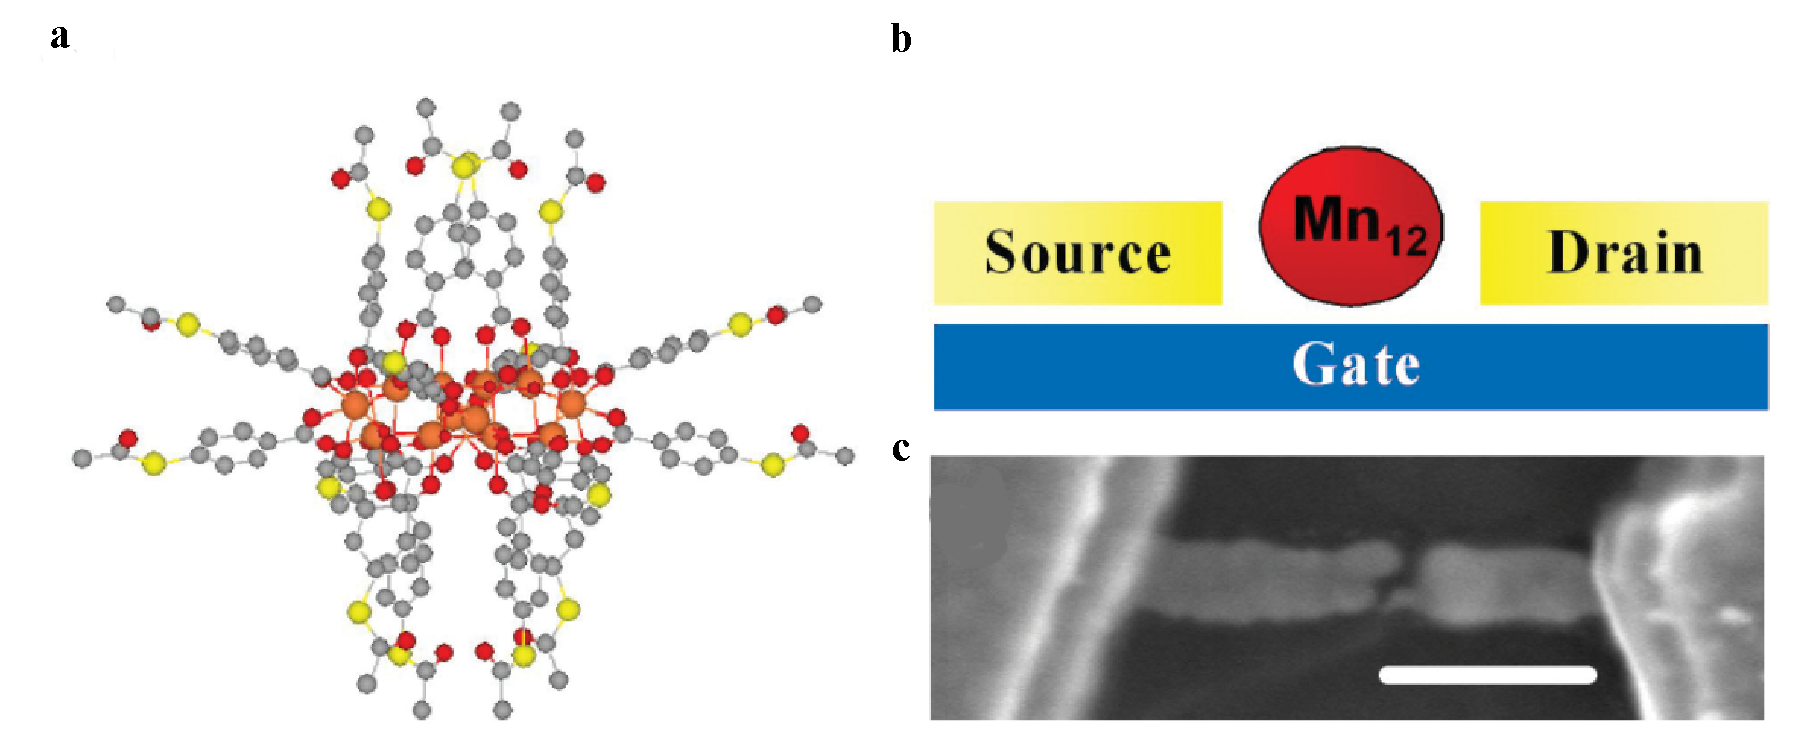
\includegraphics[scale=0.45]{Spintronique/MolSpintro/MolSpintro.pdf}
\caption{\textbf{a} : structure du Mn$_{12}$ entouré de ligands thiols favorisant l'ancrage. \textbf{b} : Représentation schématique de la molécule de Mn$_{12}$ piégée entre les électrodes. \textbf{c} : image de la jonction électromigré obtenue par microscopie électronique à balayage. Le trait blanc correspond à $200\,nm$.~(extrait de~\cite{Heersche2006}).}
\label{MolSpintro}
\end{figure}

Loin d'\^etre des échecs, ces différents travaux ont fournis un apport important au reste de la communauté, notamment concernant les critères essentiels que doivent remplir les aimants moléculaires susceptibles d'être étudiés par les techniques expérimentales actuelles. Je détaillerai ces différents critères lorsque j'introduirai le Terbium double-Decker.
 
\subsection{La spintronique dans notre groupe}
Le groupe au sein duquel j'ai effectué ma thèse a une culture ancrée dans le nano-magnétisme et le magnétisme moléculaire. Une bonne partie des efforts de la fin des années 1990 et du début des années 2000 a été consacré à l'analyse et la caractérisation de systèmes magnétiques allant de la nanoparticule au cristal moléculaire  et plus récemment, l'aimant moléculaire isolé et le spin nucléaire unique. A chaque échelle de moment magnétique correspond un dispositif de mesure, et assez logiquement, plus le moment magnétique à mesurer est faible, plus le détecteur est petit. Cette tendance est bien représentée dans la Fig.\ref{Group1}. Pour des particules macroscopiques, l'usage d'un SQUID est suffisant. Lorsque l'on veut caractériser des particules de l'ordre de quelques dizaines de nanomètre ou bien encore un cristal moléculaire, correspondant à des moments magnétiques de l'ordre de quelques milliers de $u_B$, l'usage d'un détecteur aussi sensible qu'un micro-SQUID est indispensable.


\begin{figure}
\centering 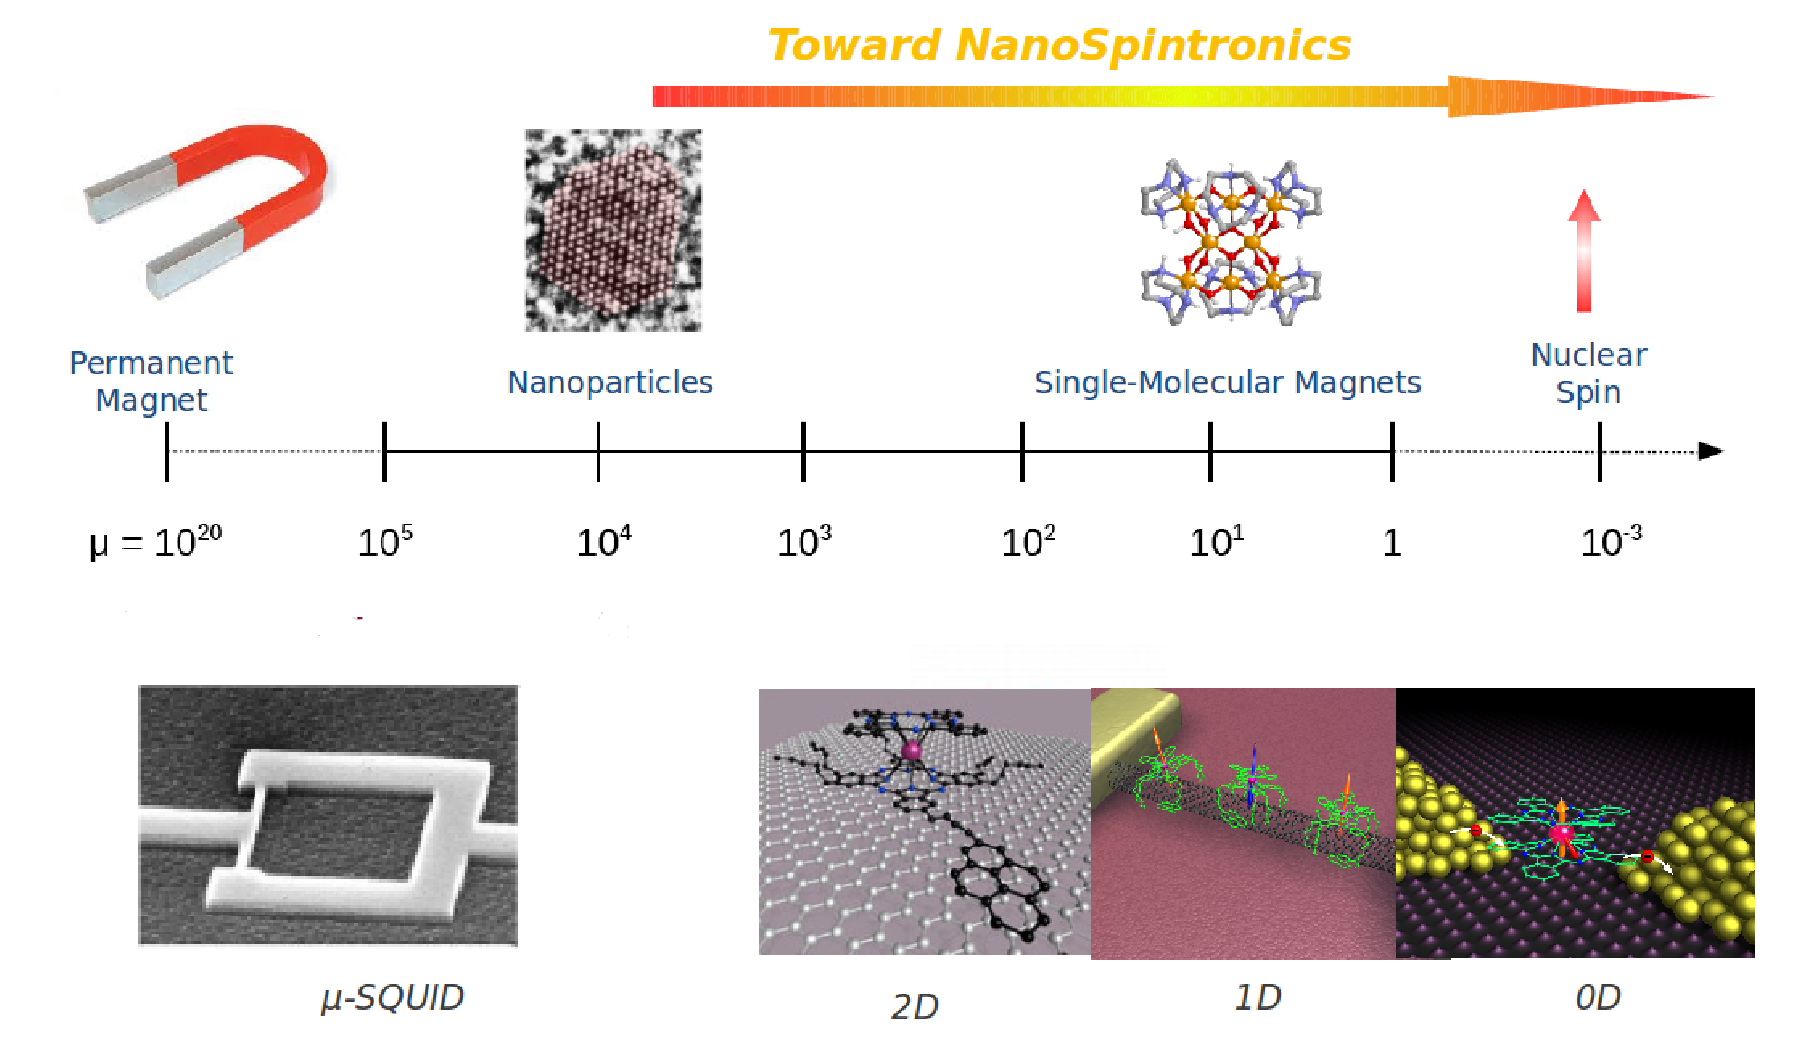
\includegraphics[scale=0.45]{Spintronique/Group1/Group1.pdf}
\caption{\'Evolution des dispositifs de détection en fonction de l'intensité du moment magnétique à mesurer.}
\label{Group1}
\end{figure}



Lorsque le moment magnétique a détecter devient très petit, de l'ordre du magnéton de Bohr, comme pour une molécule par exemple, il n'est plus vraiment possible de faire la distinction entre le détecteur et l'objet à mesurer. Il faut alors songer à fabriquer un dispositif électronique dont le fonctionnement même est influencé par le magnétisme de l'un de ses composants. Autrement dit, il faut faire appel à la spintronique moléculaire.

C'est dans ce cadre que se sont effectués les travaux conduisant à la fabrication du premier nanosquid en 2006~\cite{CleuziouJ.-P.2006}, dont les deux liens faibles supraconducteurs sont constitués par un nanotube. Ce dernier a notamment permis d'étudier l'effet Kondo dans les jonctions Josephson, et de mettre en évidence un transition $0-\pi$. Une seconde stratégie, consistant à remplir un nanotube de carbone avec des nanoparticules magnétiques, a permis de mesurer, pour la première fois, une astroide de Stoner–Wohlfarth~\cite{Cleuziou2011}.

La thématique des nanotubes ne s'est pas arrêtée aux nanoparticules, et de nouveaux dispositifs à base d'aimants moléculaires ont été développés. Ils ont donné des résultats encourageants comme dans le cas de la vanne de spin obtenue par Matias Urdampilleta~\cite{Urdampilleta2011}. Dans son expérience, un tube a été relié à deux électrodes, une grille permettant de faire varier son potentiel. Un solution contenant des molécules de TbPc$_{2}$ a ensuite été déposée, puis l'échantillon a été disposé dans un frigo à dilution. Les résultats ont mis en évidence un comportement de type vanne de spin, et une analyse fine des mesures a permis de déterminer que les rôles de polariseur et d'analyseur étaient joués par deux aimants moléculaires. Il s'agit là du premier dispositif de spintronique moléculaire mettant en jeux des aimants moléculaires. Il est assez amusant de constater que le premier dispositif qui a permis de mettre la spintronique sur le devant de la scène, soit également le premier a être réalisé en spintronique moléculaire.

\begin{figure}
\centering 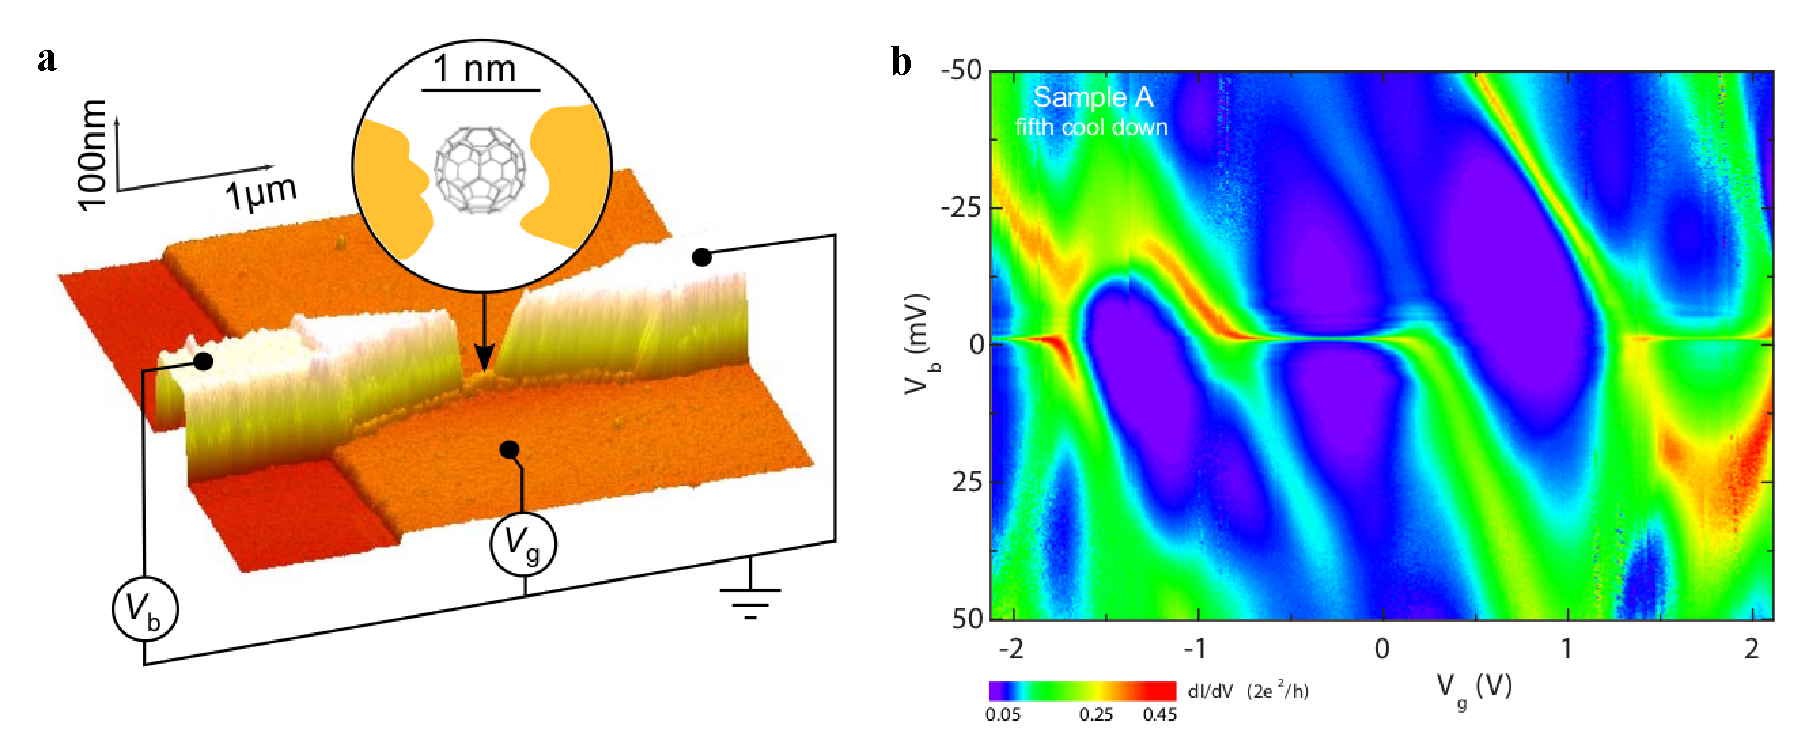
\includegraphics[scale=0.45]{Spintronique/RochC60/RochC60.pdf}
\caption{\textbf{a} : image obtenue par microscopie électronique à balayage illustrant la géométrie d'un transistor moléculaire obtenu par électromigration. \textbf{b} : spectroscopie en cotunneling obtenue en mesurant la conductance différentielle de l'échantillon en fonction de la tension source-drain $V_{\rm{ds}}$ et du champ magnétique $B$ pour une tension de grille $V_{\rm{g}}$ fixée. \textbf{c} : vue d'artiste de la molécule de N@C$_{60}$. \textbf{d} : configuration magnétique de cette dernière en fonction de son état de charge~(extrait de \cite{Roch2011}).}
\label{RochC60}
\end{figure}

En parallèle, et en collaboration avec l'université et l'institut de nanosciences de Modène, un dispositif hybride graphène-SMM a été mis au point. Celui-ci a été obtenu en gravant au sein d'une feuille de graphène, par lithographie électronique, une nanoconstriction. Ensuite, une solution contenant des molécule de TbPc$_{2}$ a été déposée~\cite{Candini2011}. Le système hybride ainsi obtenu, a permis de mettre en évidence la signature d'un aimants moléculaire à l'aide d'une mesure en conductance du système.

Afin d'améliorer encore la sensibilité de nos dispositifs, nous nous sommes intéressés à la fabrication de transistors à molécule unique. Pour cela, notre groupe a développé, à partir des travaux de H. Park~\cite{Park1999}, sa propre technique d'électromigration basée sur une boucle de contre-réaction rapide. Ces travaux ont d'abord permis la réalisation d'un transistor moléculaire à base de C$_{60}$. Celui-ci à conduit à l'observation de nombreux phénomènes quantiques tels que l'effet Kondo sous-écranté~\cite{Roch2009} ou bien encore la transition de phase quantique~\cite{Roch2008}. Puis, en collaboration avec W. Harneit, nous avons étudié la molécule de N@C$_{60}$~\cite{Roch2011}, confirmant les résultats obtenus quelques temps plus tôt par D.C. Raplh, et complétant ses observations par des mesures en cotunneling. L'ensemble de ces travaux peut être trouvé dans la thèse de Nicolas Roch.

%\begin{figure}[H]
%\centering \includegraphics[scale=0.45]{Spintronique/Group2/Group2.pdf}
%\caption{Vue d'artiste de la vanne de spin moléculaire~(\textbf{a}) et du transistor moléculaire~(\textbf{b}) à base de TbPc$_{2}$.}
%\label{Group2}
%\end{figure}

Cette analyse nous a également permis d'identifier les faiblesses de notre dispositif expérimental. Il nous fallait ajouter deux axes magnétiques pour explorer les trois directions de l'espace, mais également être capable de balayer le champ beaucoup plus rapidement : avec des vitesses de plusieurs centaines de milli-Tesla par seconde. Fort de l'expérience du groupe dans le domaine du nanomagnétisme, un dispositif mettant en jeux deux bobines de faible inductance et un système de dilution rotative a été développé rapidement au sein du laboratoire. Ce dispositif a permis d'obtenir les résultats que je vais vous présenter dans cette thèse.


\chapter{Fabrication d'un transistor moléculaire}

L'une des étapes essentielles dans la caractérisation d'un aimant moléculaire consiste a fabriquer un transistor à molécule unique~(SMT - Single Molecule Transistor). Du fait de la petite taille de ces dernières~($1\,nm$ environ), il est impossible de faire appel à des techniques lithographiques classiques. Nous avons déjà abordé les différentes solutions développées dans le cadre de la spintronique. Nous avons fait le choix d'utiliser la technique d'électromigration développé par H. Park \textit{et al.} avec quelques adaptations.

Deux éléments sont prépondérants dans la qualité d'un SMT : l’efficacité de la grille et la bonne qualité des interstices. Nous présenterons dans une première partie les différentes étapes nous permettant d'obtenir une grille efficace, après avoir défini les critères définissant cette efficacité. Ensuite, nous montrerons comment il est possible, en utilisant le phénomène d'électromigration, de produire des interstices nanométriques. Nous verrons enfin la technique de déposition ainsi que les premières étapes de caractérisation électrique des dispositifs obtenus.


\begin{figure}
\parbox{6.5cm}{
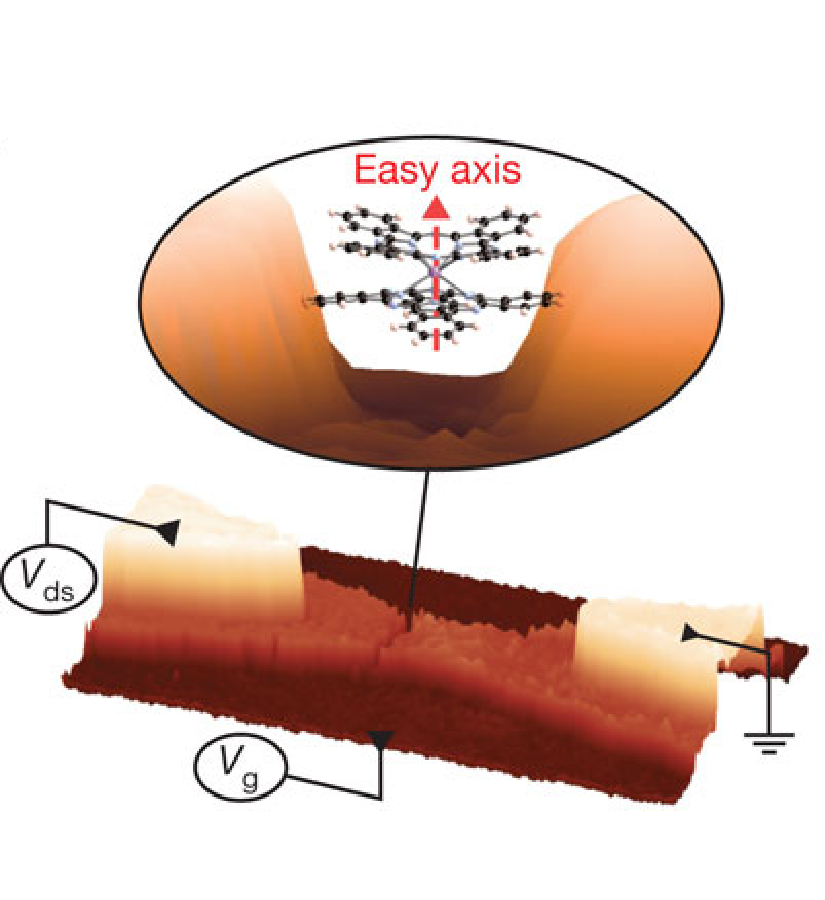
\includegraphics[scale=0.45]{Fabrication/ImageTrans/ImageTrans.pdf} 
}
\parbox{7cm}{\caption{Extrapolation 3D d'une image obtenue par microscopie électronique à balayage. Elle correspond à la structure finale que l'on souhaite obtenir : les électrodes de source et de drain, l'électrode de grille, ainsi qu'un interstice nanométrique dans lequel une molécule est piégée~(extrait de~\cite{Vincent2012}).}
\label{ImageTrans}
}
\end{figure}

\section{Réalisation d'une grille locale}
La grille est un élément essentiel du transistor et c'est également vrai d'un transistor moléculaire~\cite{Datta2009,Zant2006}. Dans ce dernier cas, elle permet notamment de moduler le potentiel chimique de la molécule allant jusqu'à modifier son état de charge~\cite{Beenakker1991,Wiel2002,Hanson2007}~(cf annexe sur le transport mésoscopique). Elle permet également de contrôler la conductance du système~(avec le concours de la tension source-drain), et donc de choisir des points de fonctionnement adaptés. Nous détaillerons ce dernier point dans le chapitre résultat. 

L'efficacité intrinsèque d'une grille peut être résumée en un seul critère~:~la charge induite. Celle-ci s'exprime simplement par $Q = CV_g^{max}$ où $Q$ est le charge induite et $C$ est la capacité associée à la grille, $V_g^{max}$ étant la tension maximale applicable à la grille. Elle dépend essentiellement de trois paramètres physiques : le champ électrique maximum applicable, l'épaisseur et la permittivité de l'oxyde~\cite{Biercuk2003}. 

Outre les paramètres que l'on vient de voir, il existe plusieurs géométries de grille susceptibles d'avoir une influence sur l’efficacité de cette dernière. On peut identifier trois géométries : la grille au-dessus ou  ``\textit{top-gate}'', la grille latérale et la grille arrière ou  ``\textit{back-gate}''.

\subsection{Les différentes géométries}
Je ne donnerai ici qu'une rapide présentation des différentes grilles existantes. Une comparaison plus détaillée entre ces différentes géométries est disponible dans la thèse d'Aurore Mangin~\cite{Aurore2009}.

\begin{figure}
\centering 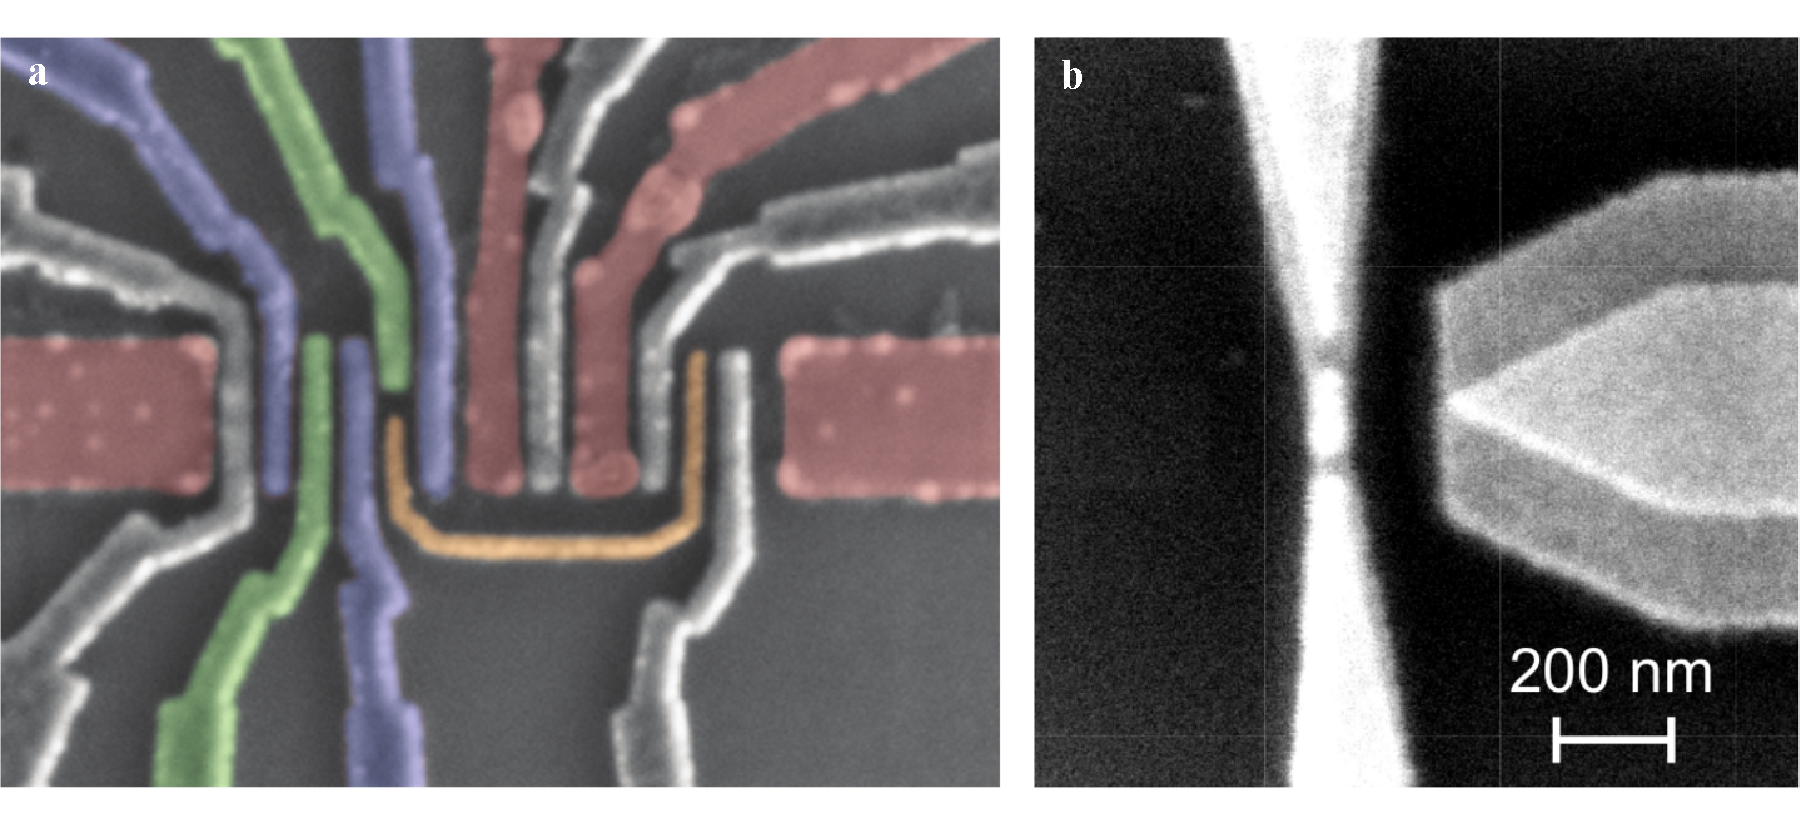
\includegraphics[scale=0.45]{Fabrication/Gateconf/GateConf.pdf}
\caption{Images obtenues par microscopie électronique à balayage. \textbf{a} : nanotube sur lequel on est venu positionner 9 grilles afin de réaliser un double point quantique ainsi qu'un détecteur de charge ~(extrait de \cite{Churchill2009}). \textbf{b} : configuration en grille latérale réalisée dans la cadre de jonctions électromigrés~(extrait de~\cite{Aurore2009}).}
\label{GateConf}
\end{figure}


\subsubsection{La ``\textit{top-gate"}}
Cette configuration est utilisée dans le cas des transistors à effet de champ conventionnels. On la retrouve également dans les dispositifs expérimentaux faisant appel à des nanofils~\cite{Fasth2005} ou bien encore à des nanotubes~\cite{Javey2002}~(cf Fig.\ref{GateConf}.\textbf{a}). Elle a également pu être implémentée dans le cas de nanotubes suspendus donnant des résultats plus que convaincants~\cite{Leturcq2009}.

Cette configuration est cependant difficilement compatible avec l'électromigration. En effet, celle-ci est effectuée après les étapes de lithographie, ce qui serait impossible si le fil d'or était recouvert par une grille. Pour produire une grille compatible avec l'électromigration, il faut se tourner vers d'autres géométries comme la configuration latérale.

\subsubsection{La grille latérale}
Cette configuration consiste à placer la grille latéralement vis à vis du gap obtenu par électromigration~\cite{Mangin2009}~(cf Fig.\ref{GateConf}.\textbf{b}). Accompagnée d'une grille arrière, elle permet d'avoir deux moyens d'action sur le potentiel chimique de la molécule située dans la gap. 

Il est en revanche très difficile de contr\^oler précisément la position de cette grille, et elle se trouve donc souvent située à plusieurs dizaines de nanomètres du gap. De plus, le r\^ole de l'oxyde est dans ce cas joué par l'air, qui possède une permittivité proche de l'unité. Cette configuration abouti donc, de manière générale, à une grille moins efficace que la configuration grille arrière~\cite{Aurore2009} que nous allons voir maintenant.


\subsubsection{La grille arrière}
Dans cette configuration, la grille se situe sous le dispositif. Elle a notamment été adoptée pour la réalisation du premier transistor à molécule unique~\cite{Park2000}. Elle est bien s\^ur compatible avec l'électromigration et, implémentée en grille locale, elle permet d'obtenir des grilles très efficaces. Pour ces raisons, nous avons choisi d’adopter cette configuration pour nos échantillons. De plus, sa fabrication peut \^etre grandement facilitée par l'utilisation de la technique ALD~(Atomic Layer Deposition - dép\^ot par couche atomique) que nous allons présenter dans la suite.


\subsection{Création de l'électrode de grille}

La première étape de la fabrication de notre grille locale consiste en l'obtention de l'électrode de grille. Compte tenu des tailles caractéristiques de cette dernière, cette électrode peut \^etre obtenue à l'aide d'une lithographie optique ultra-violet profond (DUV - Deep Ulta-Violet). A cette fin, une méthode bicouche LOR3A/UV3 est utilisée en suivant les instructions du Tab.\ref{tab_recette}, avec pour seule différence, l'épaisseur d'or déposée : $20\,nm$.

\begin{table}
\begin{center}
\begin{tabular}{|p{0.5cm}|p{4cm}|p{4cm}|p{3cm}|}
  \hline
\,& \textbf{étape} & \textbf{procédé} & \textbf{paramètres} \tabularnewline
\hline
1 &  nettoyage du wafer & acétone, ethanol, isopropanol et plasma oxygène (RIE)& $2\,$min \tabularnewline
\hline
 2 & étalement de LOR 3A pour une épaisseur de $400\,$nm& tournette & v\,:\,$2000\,$tr.min$^{-1}$, a\,:\,$2000\,$tr.min$^{-2}$, t\,:\,$30\,$s \tabularnewline
\hline
 3 & recuit & plaque chauffante & $1\,$min à $170\,\degres$C \tabularnewline
\hline
4 & étalement de UV3 & tournette & v\,:\,$4000\,$tr.min$^{-1}$, a\,:\,$2000\,$tr.min$^{-2}$, t\,:\,$30\,$s \tabularnewline
\hline
5 & recuit & plaque chauffante & $1\,$min à $130\,\degres$C \tabularnewline
\hline
6 & insolation & aligneur dUV MJB3 & $5.5\,$s à $0.3\,$mW.cm$^{-2}$\tabularnewline
\hline
7 & recuisson & plaque chauffante & $1\,$min à $130\,\degres$C \tabularnewline
\hline
8 & développement & MF-CD-26 & $30-40\,$s\tabularnewline
\hline
9 & neutralisation du développeur & eau DI & $1\,$min\tabularnewline
\hline
10 & dépôt de la couche d'accroche métallique & évaporateur à canon à électron PLASSYS & $5\,$nm de Ti à $0.1\,$nm.s$^{-1}$ \tabularnewline
\hline
11 & dépôt de la couche métallique principale & évaporateur à canon à électron PLASSYS & $100\,$nm de Au à $0.1\,$nm.s$^{-1}$ \tabularnewline
\hline
12 & \textit{lift-off} & acétone & $10\,$min à $1\,$h, on peut l'assister par ultra-son à $80\%$ de la puissance maximum. \tabularnewline
\hline
 13 & dissolution de LOR3A & PG-Remover & $1\,$h à $80\,\degres$C \tabularnewline
\hline
14 & rinçage & acétone et isopropanol & $1\,$min de chaque sous la pissette\tabularnewline
\hline
15 & séchage & azote sec & wafer posé sur du papier absorbant, pistolet à la verticale du wafer, ne pas toucher le wafer avec des pinces\tabularnewline
\hline
16 & nettoyage & plasma oxygène (RIE)& $10\,$min\tabularnewline
\hline
\end{tabular}
\caption{Recette du bicouche LOR3A/UV3 : celle-ci permet de ne plus avoir d'effet de bord lors des lift-offs.}
\label{tab_recette}
\end{center}
\end{table}


Cette étape permet également d'obtenir les marques d'alignements nécessaires à la fabrication des lignes d'amenés. Une première série de marques~(cf carré bleu de la Fig.\ref{FinalResult}.\textbf{a}) permet d'effectuer un alignement grossier. Ce dernier est ensuite affiné à l'aide d'une deuxième série de repères~(cf carré vert de la Fig.\ref{FinalResult}.\textbf{a}).

La technique bicouche a été préférée à la technique usuelle monocouche, car elle a l'avantage de prévenir la formation de bords lors de l'étape de lift-off~(cf Fig.\ref{lift-off}). En effet, la présence de ces bords pourrait entraîner une perte de contact entre la jonction et le plot correspondant, lors du passage de marche~(i.e. lorsque la ligne d'amené, réalisée par lithographie électronique, passe de la surface de silicium à la grille, la hauteur de marche étant donnée par l'épaisseur de la grille).


\begin{figure}
\centering 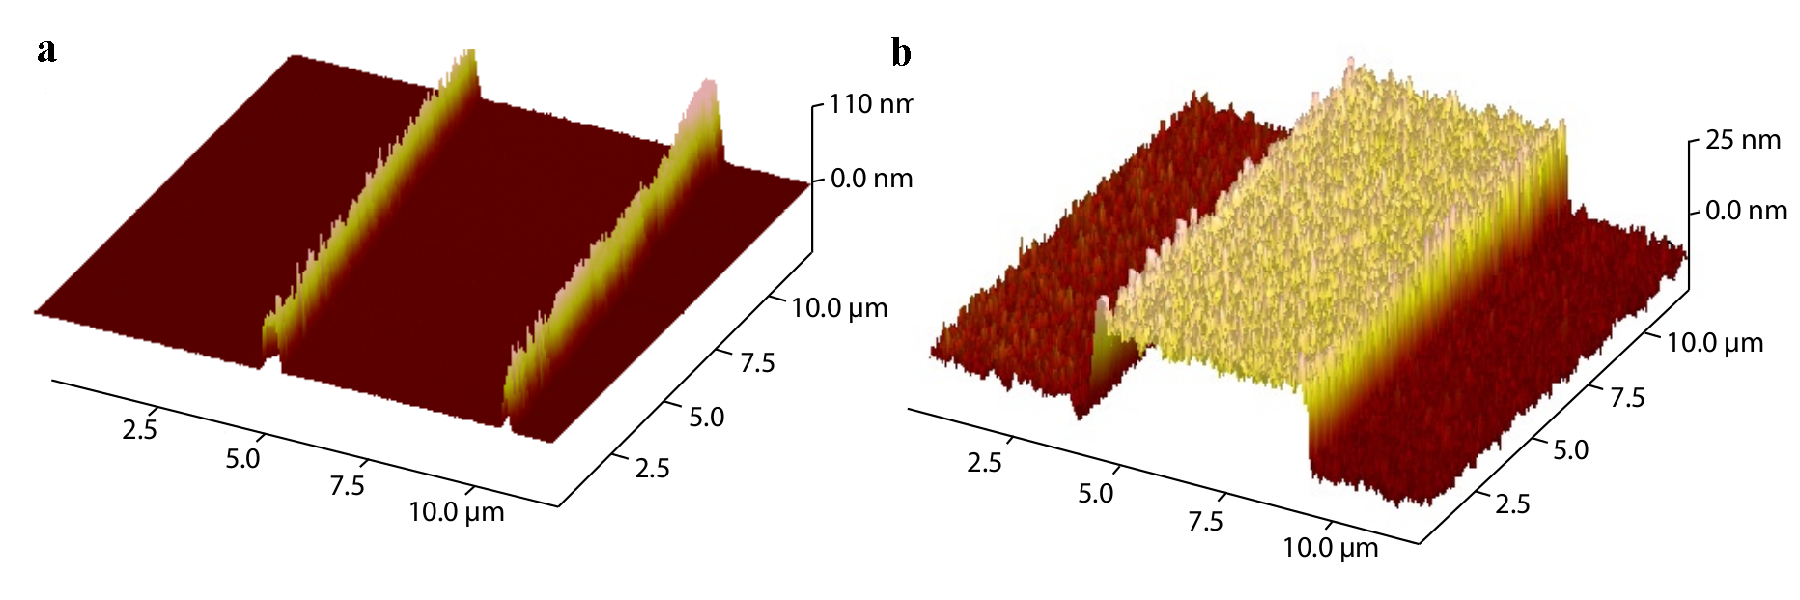
\includegraphics[scale=0.45]{Fabrication/BatmanGrille/BatmanGrille.pdf}
\caption{\textbf{a} : image AFM d'une électrode de grille présentant des bords trop relevés d\^u fait d'un problème de lift-off, obtenue par une technique monocouche. \textbf{b} : image AFM montrant une électrode de grille après lift-off ne présentant pas d'anomalie après lift-off obtenue par la la technique bicouche~(extrait de~\cite{RochPhD}).}
\label{lift-off}
\end{figure}

Cette première étape est suivie du dépôt d'oxyde par une méthode de dépôt par couche atomique ou ALD~(Atomic Layer Déposition) que nous allons détailler maintenant.

\subsection{Le dép\^ot par ALD}

Comme nous l'avons déjà précisé en introduction, le choix de l'oxyde est très important et, en particulier, la permittivité de ce dernier doit être la plus élevée possible.

Parmi les oxydes à haute permittivité, les plus couramment utilisés sont l'alumine~($\kappa \sim 8$), l'hafnia~($\kappa \sim 17$) et l'oxyde de zirconium~($\kappa \sim 26$)~\cite{Biercuk2003}. De manière générale, le premier est obtenu par dépôt d'une électrode d'aluminium, puis exposition à une atmosphère riche en oxygène, ou bien par ALD. Les deux derniers sont en général obtenus par ALD ou, plus rarement, par MOCVD~(Metalorganic Chemical Vapour Deposition). Lorsque je suis arrivé en thèse, la technique par oxydation naturelle était en usage. Bien que relativement facile à mettre en œuvre, il est difficile de connaître avec exactitude l'épaisseur d'oxyde. De plus, nous avons observé une grande variabilité dans la qualité des grilles obtenues par ce procédé.

Nous avons donc développé un nouveau procédé inspiré de~\cite{Biercuk2003}, en utilisant une méthode ALD, nous permettant d'obtenir une grille avec un oxyde de $8\,nm$ environs. Parmi les trois oxydes précédemment cités, nous avons choisi l'oxyde d'hafnium. Celui si à l'avantage d'être fortement documenté et présente des performances supérieures à l'alumine pour ce qui est de la charge induite~\cite{Biercuk2003}. 

La technique d'ALD originellement appelée ALE~(pour Atomic Layer Epitaxie) a été brevetée dans les années 1970, et remise au goût du jour pour les besoins toujours plus grands de la microélectronique~\cite{Leskelae2003}. Elle consiste en une succession de deux réactions auto-limitantes, aboutissant à la formation d'un oxyde comme le montre la Fig.\ref{ALD}.

\begin{figure}
\centering 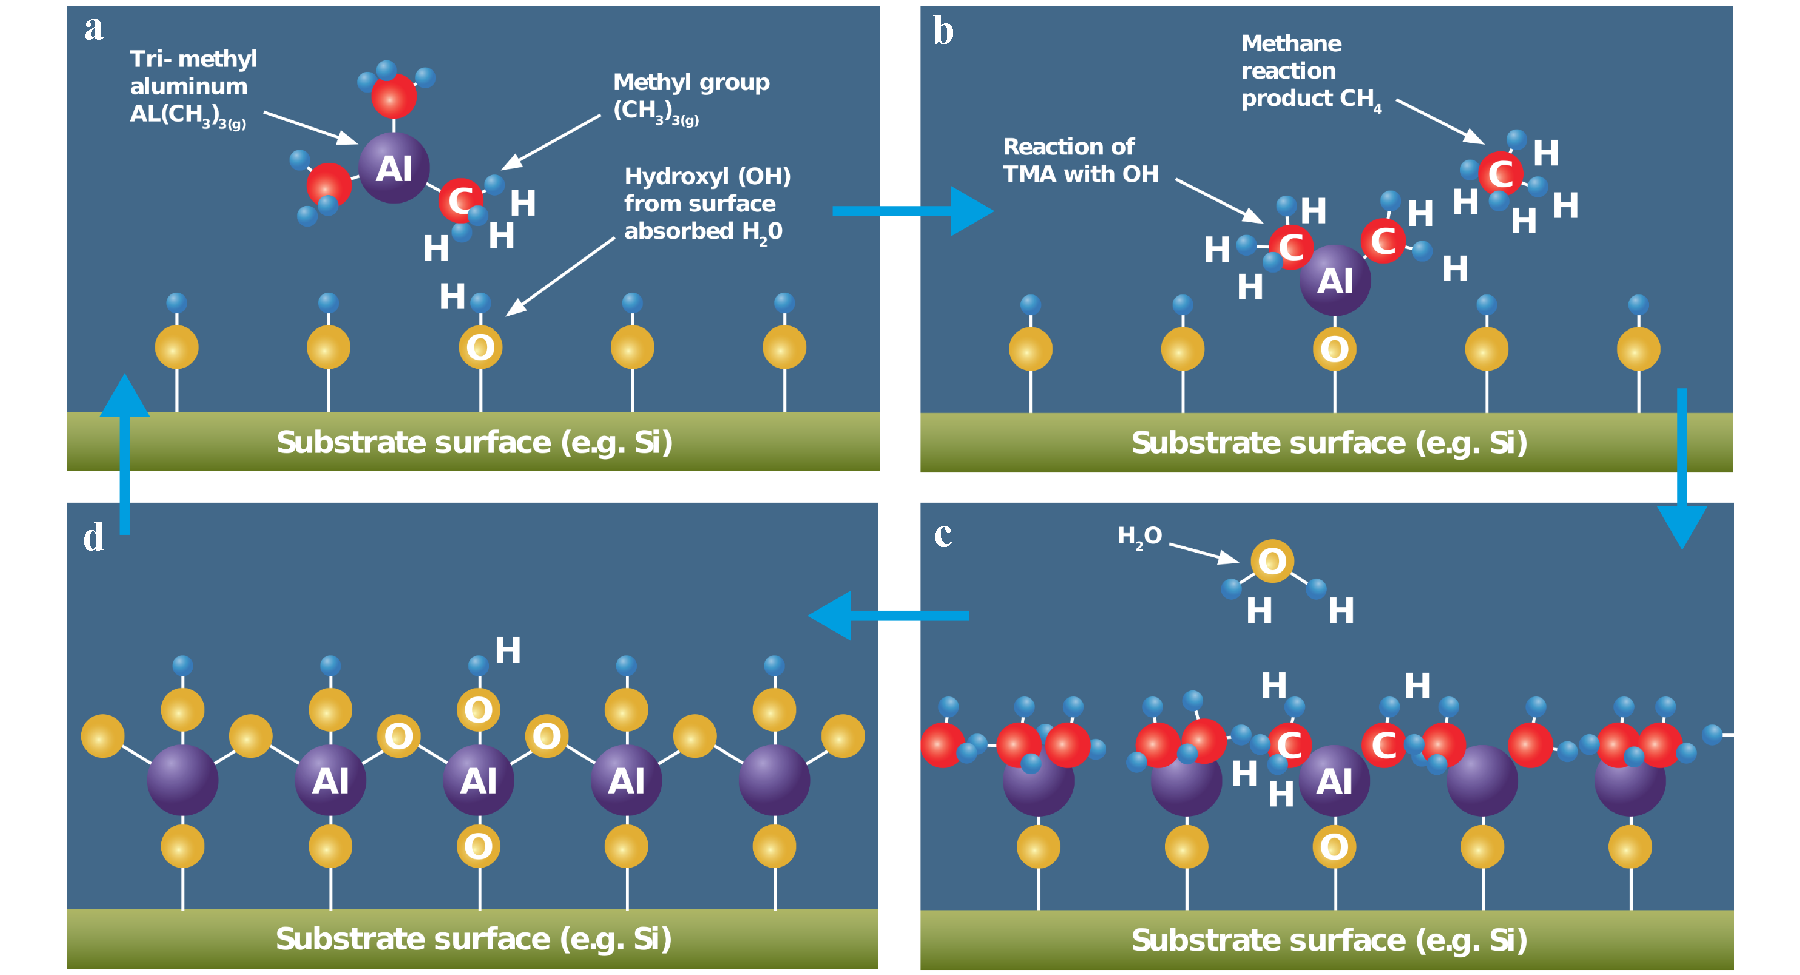
\includegraphics[scale=0.45]{Fabrication/ALD/ALD.pdf}
\caption{Première étape du cycle ALD : le premier précurseur, ici du Al(CH$_3$)$_{3(g)}$, se fixe à la surface~(\textbf{a}) et les produits issues la réaction de fixation sont évacués par un flux de gaz inerte~(\textbf{b}). Dans un deuxième temps, de l'eau est injectée et réagi avec la première couche de précurseur~(\textbf{c}) pour former une couche atomique d'oxyde~(\textbf{d}). Le cycle se répète ensuite à raison d'une couche atomique par cycle. (extrait du site CambrigeNanoTech)}
\label{ALD}
\end{figure}


Le premier avantage de la technique est sa facilité de mise en œuvre. Le contrôle du procédé, couche par couche, permet de choisir l'épaisseur d'oxyde déposée avec une grande précision. De plus, la nature de ce dernier est uniquement déterminée par les précurseurs utilisés, ce qui donne un large choix de matériaux. Afin d'obtenir un oxyde de qualité pour les applications électroniques, celui-ci doit remplir deux critères : il doit contenir peu d'impuretés et être de préférence amorphe~\cite{Kim2003}.

\begin{table}
\begin{center}
\begin{tabular}{|p{0.5cm}|p{6cm}|p{6cm}|}
\hline
\multicolumn{3}{|c|}{\textbf{Réglages}} \tabularnewline
\hline
\multicolumn{2}{|l|}{\textbf{élement}} & \textbf{paramètres} \tabularnewline
\hline
\multicolumn{2}{|l|}{température du précurseur} & $90\, \degres C$ \tabularnewline
\hline
\multicolumn{2}{|l|}{température du \textit{Tee}} & $150\, \degres C$ \tabularnewline
\hline
\multicolumn{2}{|l|}{température de la chambre~(\textit{inner} et \textit{outer})} & $100\, \degres C$ \tabularnewline
\hline
\multicolumn{2}{|l|}{température du \textit{Bellow}} & $150\, \degres C$ \tabularnewline
\hline
\multicolumn{2}{|l|}{\multirow{2}{*}{flux d'azote}} & $20\, sccm$ \newline (pression d'environ $0.5\,Torr$) \tabularnewline
\hline
\hline
\multicolumn{3}{|c|}{\textbf{Procédé}} \tabularnewline
\hline
\,& \textbf{étape} & \textbf{paramètres} \tabularnewline
\hline
1 & pluse de TDMAH & $0.015\,s$ \tabularnewline
\hline
2 & temps d'attente & $120\,s$ \tabularnewline
\hline
3 & pulse d'eau & $0.015\,s$ \tabularnewline
\hline
4 & temps d'attente & $120\,s$ \tabularnewline
\hline
\end{tabular}
\caption{Paramètres et réglages du procédé ALD.}
\label{recette_ALD}
\end{center}
\end{table}



Pour remplir le premier critère, il est nécessaire de chauffer de façon suffisante le substrat, afin de désorber efficacement les déchets produits lors de la fixation du précurseur~(cf Fig.\ref{ALD}). Une structure amorphe, au contraire, est obtenue par un dép\^ot à basse température~\cite{Triyoso2004}. Cela a en plus l'avantage de rendre le procédé compatible avec une étape de lithographie~\cite{Biercuk2003}~(évitant une détérioration de la résine) et de diminuer la rugosité de l'oxyde~\cite{Triyoso2004}. Il faut donc arriver à trouver un compromis entre ces deux conditions contradictoires.

Celui-ci a été trouvé en laissant un délai conséquent entre les différentes étapes du dépôt, permettant aux produits de réaction de désorber~\cite{Biercuk2003}. Cela se traduit par un temps d'attente de 2 minutes entre chaque étape de cycle. Un dépôt de 80\,cycles~(environ $8\,nm$) d'hafnia prend donc un peu plus de cinq heures~(pour les détails concernant le dépôt ALD, le lecteur peut se référer au Tab.\ref{recette_ALD}). Si ce temps peut paraître long au premier abord, il ne représente qu'un temps négligeable au regard des autres étapes, et notamment, celle de lithographie électronique que nous allons aborder maintenant.

\begin{figure}
\centering 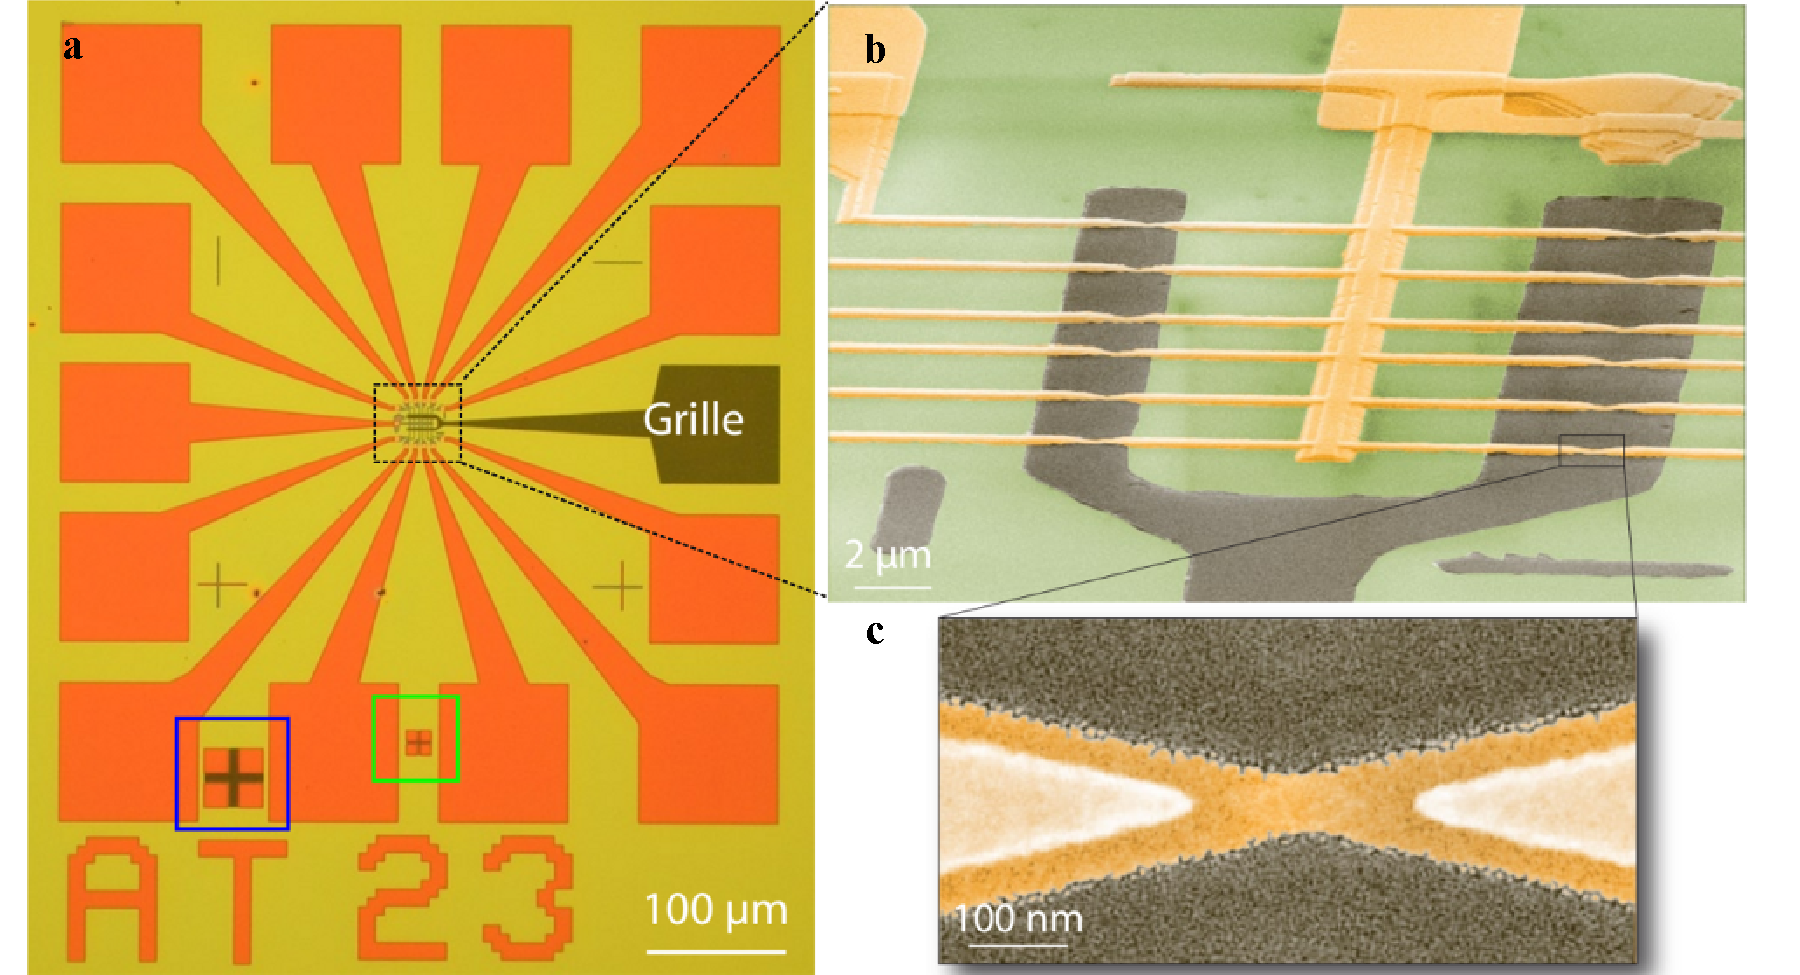
\includegraphics[scale=0.45]{Fabrication/FinalResult/FinalResult.pdf}
\caption{\textbf{a} : Échantillon après les deux étapes de lithographie optique. Les lignes d'amené de courant sont visibles en orange et la grille locale en gris. Les deux carrés repèrent les marques d'alignement. \textbf{b} : Image obtenue par microscopie électronique à balayage montrant la structure centrale de nos échantillons. \textbf{c} : grossissement présentant une constriction obtenue à l'aide de l'évaporation sous angle. La grille, colorée en gris, est clairement visible au centre (extrait de \cite{RochPhD}).}
\label{FinalResult}
\end{figure}


\section{Réalisation d'un nanofil}

Afin de réaliser les nanofils d'or, on procède en deux étapes. Dans la première, une lithographie optique est effectuée afin d'obtenir les plots de connexion. Dans la seconde, une lithographie électronique est réalisée en vue de la fabrication des nanofils.

\subsection{Lithographie optique}

Cette étape de lithographie vise à fabriquer les plots d'or nécessaires à la micro-soudure de notre échantillon, ainsi que les lignes d'amené de courant~(cf partie orange de la Fig.\ref{FinalResult}.\textbf{a}). La recette du Tab.\ref{tab_recette}  est utilisée pour obtenir un dép\^ot de 80$\,nm$ d'or avec une couche d'accroche en titane.

Le résultat final est présenté dans la Fig.\ref{FinalResult}.\textbf{a} où la partie orange désigne les lignes d'amené de courant et la partie grise la grille locale. La partie centrale va venir accueillir les nanofils d'or comme nous allons le voir dans la suite.


\subsection{Lithographie électronique}



Comme nous l'avons présenté dans l'introduction, notre méthode de fabrication repose sur la technique d'électromigration. Cette dernière, pour fonctionner correctement, a besoin d'\^etre opérée sur des fils d'or très fins, présentant une section de quelques dizaines de nanomètres, pour une épaisseur de quelques nanomètres en ce qui concerne la partie la plus fine~(cf Fig.\ref{EvapAngle}). 

\begin{figure}[h!]
\centering 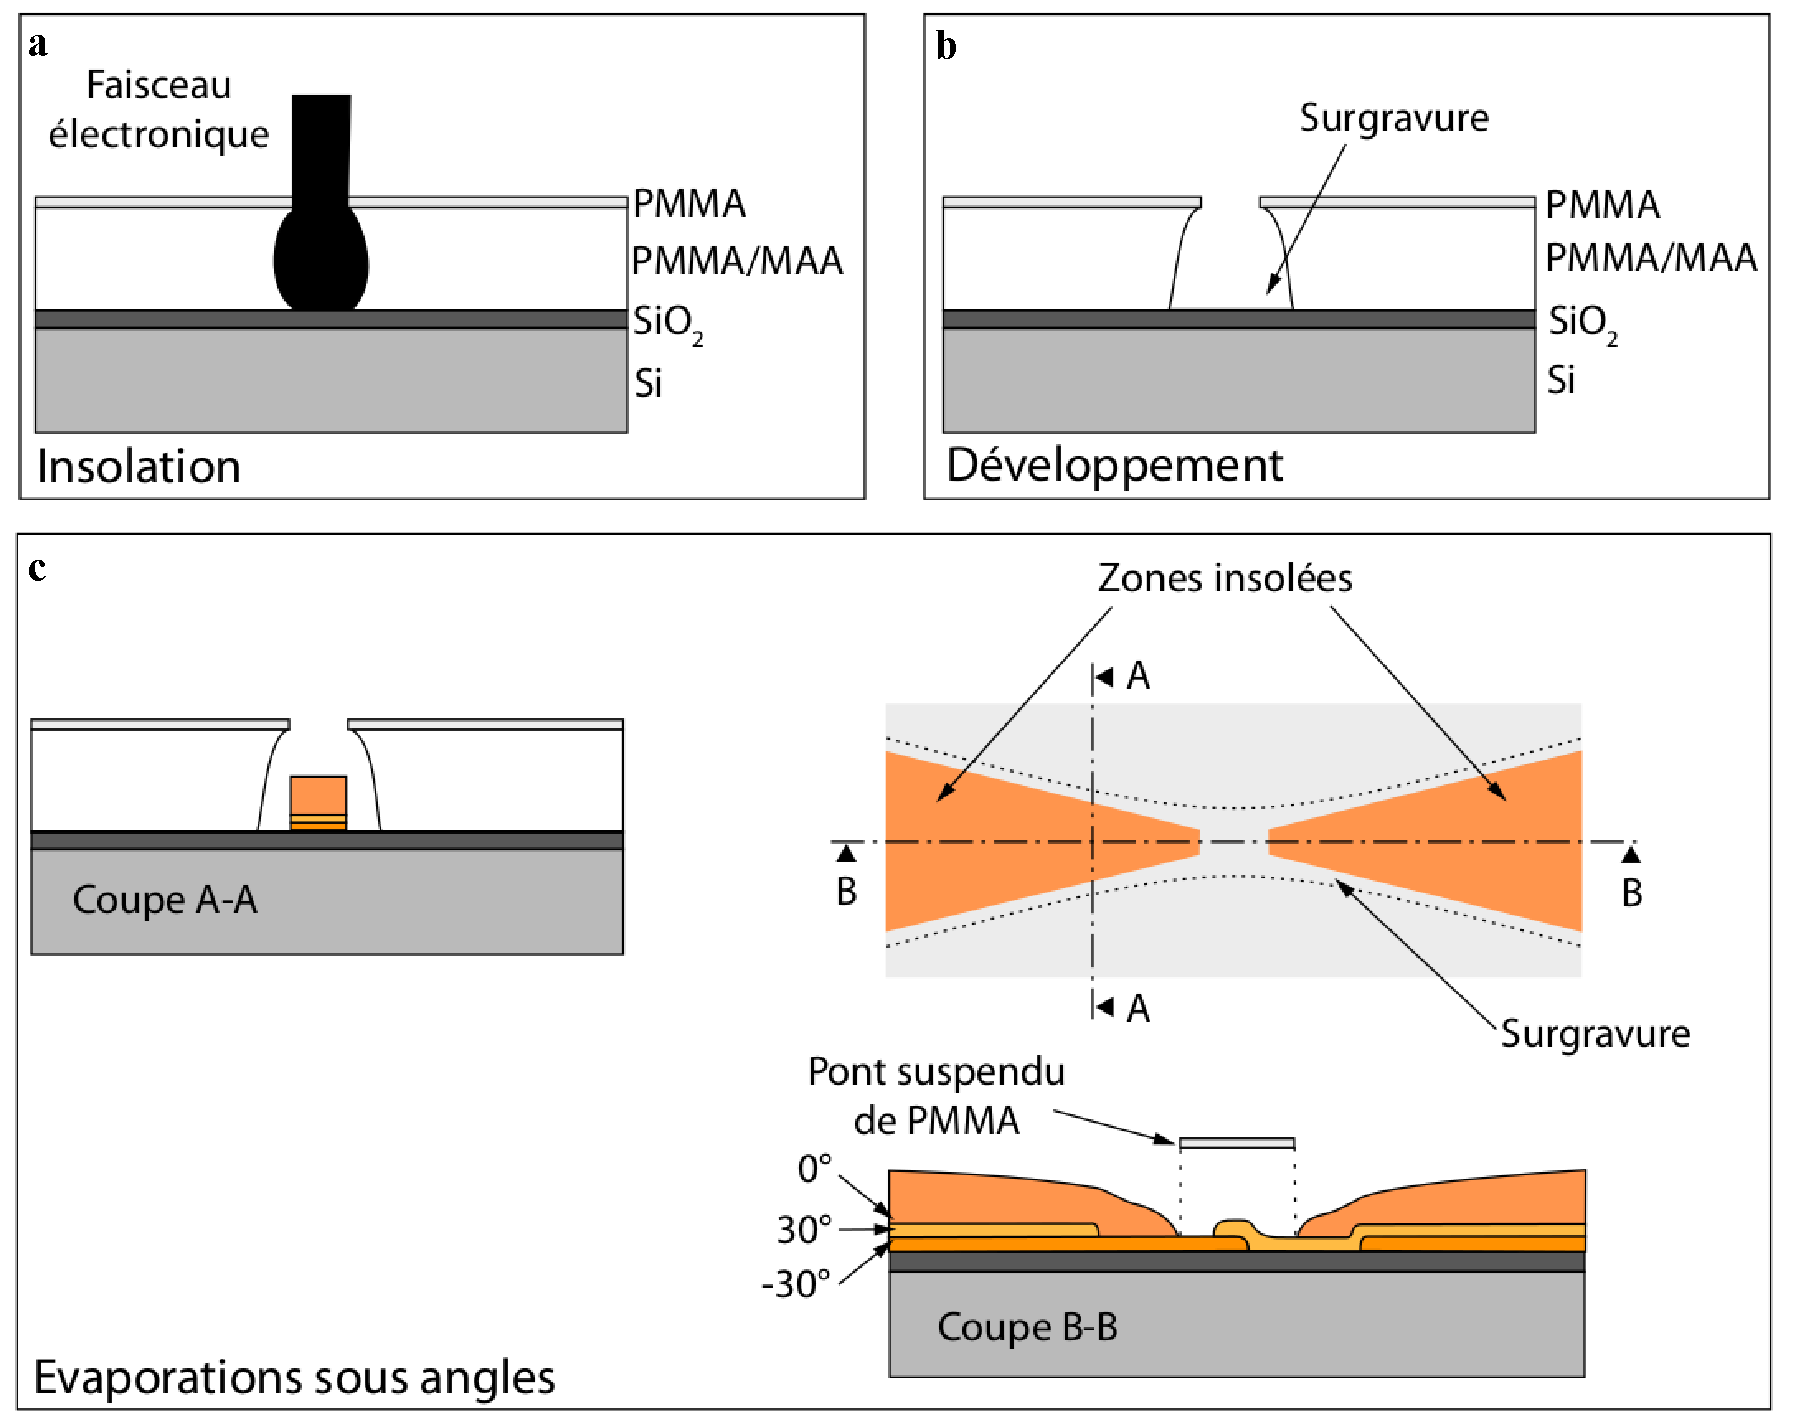
\includegraphics[scale=0.45]{Fabrication/EvapAngle/EvapAngle.pdf}
\caption{\textbf{a} : Insolation par lithographie électronique de la bicouche de résine. La partie la plus proche du substrat~(PMMA/MAA) se trouve plus insolée de par une plus grande sensibilité aux électrons et la présence des électrons rétrodiffusés. \textbf{b} : résultats après développement montrant clairement la surgravure générée par la surexposition de la partie basse. \textbf{c} : Evaporation sous angle : différentes couleurs représentent les différents angles d'évaporation (-30$\,\degres$, 0$\,\degres$ et 30$\,\degres$ - extrait de \cite{RochPhD}).}
\label{EvapAngle}
\end{figure}

Le nanofil va également avoir un impact sur le couplage de la molécule à la grille. Cette dépendance se fait de deux manières. Tout d'abord, la forme de pointe, donnée au niveau de la partie fine du nanofil, va minimiser l'écrantage une fois le gap obtenu. Une analyse des différents paramètres influençant cet écrantage est disponible dans~\cite{Datta2009}. Ensuite, en ayant une largeur faible, la surface en vis à vis avec la grille, et donc le risque de fuite de grille à travers un défaut de l'oxyde, est minimisée, augmentant la tension maximale applicable.

\begin{table}
\begin{center}
\begin{tabular}{|p{0.5cm}|p{4cm}|p{4cm}|p{3cm}|}
  \hline
\,& \textbf{étape} & \textbf{procédé} & \textbf{paramètres} \tabularnewline
\hline
1 &  dép\^ot de résine PMMA/MMA 2\,\% en masse & tournette & v\,:\,$6000\,$tr.min$^{-1}$, a\,:\,$4000\,$tr.min$^{-2}$, t\,:\,$30\,$s 
\tabularnewline
\hline
 2 & recuit (softbake) & plaque chauffante  & 5 minutes à 200$\, \degres C$ 
\tabularnewline
\hline
 3 & dépôt de résine PMMA 33\% en masse & tournette & v\,:\,$1400\,$tr.min$^{-1}$, a\,:\,$2000\,$tr.min$^{-2}$, t\,:\,$30\,$s \tabularnewline
\hline
4 & recuit & plaque chauffante & 5 minutes à 180$\, \degres C$
\tabularnewline
\hline
5 & insolation & MEB & dose de 240\,$\mu C.cm^{-2}$
\tabularnewline
\hline
6 & développement & becher MIBK/IPA ($1:3$) & 30 secondes
\tabularnewline
\hline
7 & rinçage & bécher IPA & 2 secondes
\tabularnewline
\hline
8 & surdéveloppement & bécher IPA & 1\,minute
\tabularnewline
\hline
9 & neutralisation du développeur &bécher d'eau désionisée & $1\,$minute\tabularnewline
\hline
10 & dép\^ot de la couche d'accroche & évaporateur à canon à électron PLASSYS & $3\,$nm de Ti à $0.05\,$nm.s$^{-1}$, angle=$0\,\degres$
\tabularnewline
\hline
11 & dépôt de la constriction & évaporateur à canon à électron PLASSYS & $10\,$nm de Au à $0.03\,$nm.s$^{-1}$, angle=$\pm 30\degres$
\tabularnewline
\hline
12 &  dépôt des nanofils &  évaporateur à canon à électron PLASSYS  &  $80\,$nm de Au à $0.15\,$nm.s$^{-1}$, angle=$\pm 0\degres$
\tabularnewline
\hline
 13 & lift-off & bécher d'acétone & 1\,heure minimum 
\tabularnewline
\hline
14 & rinçage & acétone, éthanol et isopropanol & 
\tabularnewline
\hline
15 & séchage & azote sec & 
\tabularnewline
\hline
16 & nettoyage & plasma oxygène (RIE)& $3\,$min\tabularnewline
\hline
\end{tabular}
\caption{Recette du bicouche PMMA/MAA : celle-ci permet d'obtenir des constrictions idéales pour l'électromigration.}
\label{tab_recette_elec}
\end{center}
\end{table}


Afin d'obtenir des fils répondant à ces critères, nous avons utilisé une méthode dite d'évaporation sous-angle. Pour cela, il faut tout d'abord déposer deux couches de résine, la partie supérieure étant constituée de PMMA et la partie inférieure de PMMA-MAA, plus sensible aux électrons~(cf Fig.\ref{EvapAngle}). On procède ensuite à la lithographie électronique puis au développement de la résine en suivant la recette du Tab.\ref{tab_recette_elec}. Du fait de la plus grande sensibilité de la partie inférieure et la présence d'électrons rétrodiffusés, on obtient une partie sur-insolée entraînant la formation d'un ``pont" comme décrit sur la Fig.\ref{EvapAngle}.

On évapore ensuite une fine couche de titane~(3$\, nm$) avec un angle de $0\,\degres$ pour constituer un couche d'accroche, puis sous un angle de $\pm30\,\degres$, $10\, nm$ d'or  constituant la constriction. Enfin, $80\,nm$ d'or sont évaporés à $0\,\degres$ afin de venir relier la constriction aux plots de connexion. Cette épaisseur doit être suffisante pour assurer un bon passage entre la partie se situant sur la grille et celle se trouvant sur la surface même du wafer. La structure finale est présentée dans la Fig.\ref{FinalResult}.\textbf{b} et \textbf{c}.


\section{Réalisation d'un interstice nanométrique}
Une fois obtenues nos constrictions métalliques, il faut procéder à la dernière étape de fabrication : l'électromigration. Celle-ci, effectuée à une température de $4\,K$, va nous permettre d'obtenir les interstices de quelques nanomètres de largeur, nécessaires à la fabrication d'un transistor moléculaire. Dans ce chapitre, nous présenterons dans un premier temps la technique d'électromigration ainsi que les différentes méthodes de mise en œuvre. Nous finirons par une description de notre technique de contre-réaction rapide à basse température.

\subsection{L'électromigration}
L'électromigration est un phénomène connu depuis plus d'un siècle maintenant~\cite{Gerardin1861}. Ce phénomène a connu un regain intérêt avec le développement de la micro-électronique, notamment parce qu'il a été identifié comme étant une cause de panne récurrente~\cite{Blech1967,Black1969}.
Il se produit lorsqu'une forte densité de courant traverse un conducteur. Les ions du réseau sont alors soumis à deux forces : la première est induite par le champ électrique générant le courant, la seconde est d\^u aux électrons qui, du fait de la diffusion, viennent céder un peu de leur moment cinétique aux ions du réseau~\cite{Ho1989}. L'action de ces deux forces se résume par la formule suivante :
\begin{eqnarray}
\textbf{F} = \textbf{F}_d + \textbf{F}_v = Z^*e\textbf{E} \nonumber
\end{eqnarray}
où $\textbf{F}_d$ est la force induite par le champ électrique et $\textbf{F}_v$ celle induite par la diffusion des électrons. Le terme $Z^*$ est en général utilisé pour représenter la charge effective des ions soumis à un champ électrique, et rend compte de l'interaction ions/électrons.

Ce phénomène a été pour la première fois utilisé en électronique moléculaire par le groupe de D.C. Ralph à Cornell~\cite{Park1999}. La technique a notamment été mis en oeuvre pour réaliser le premier transistor à molécule unique~\cite{Park2000}. Depuis, elle a connu de nombreuses évolutions comme nous allons le voir maintenant

\subsection{Etat de l'art}
On peut classer les techniques d'électromigrations en trois grandes catégories : à rampe unique, à contre-réaction et à cassure-spontanée. Une analyse plus fine des différentes méthodes est disponible dans~\cite{Girod2012}.

\subsubsection{À rampe unique}
C'est la première technique a avoir été mise en œuvre dans le domaine de l'électronique moléculaire par Park \textit{et al.}~\cite{Park1999}. Elle consiste en l'application d'une rampe de tension croissante sur une fin fil de métal (voir Fig.\ref{ParkExemp}). La simplicité de la méthode est séduisante, mais mal contrôlée, elle peut conduire à une destruction de la jonction, notamment dû au chauffage induit par effet Joule.

\begin{figure}
\parbox{7cm}{
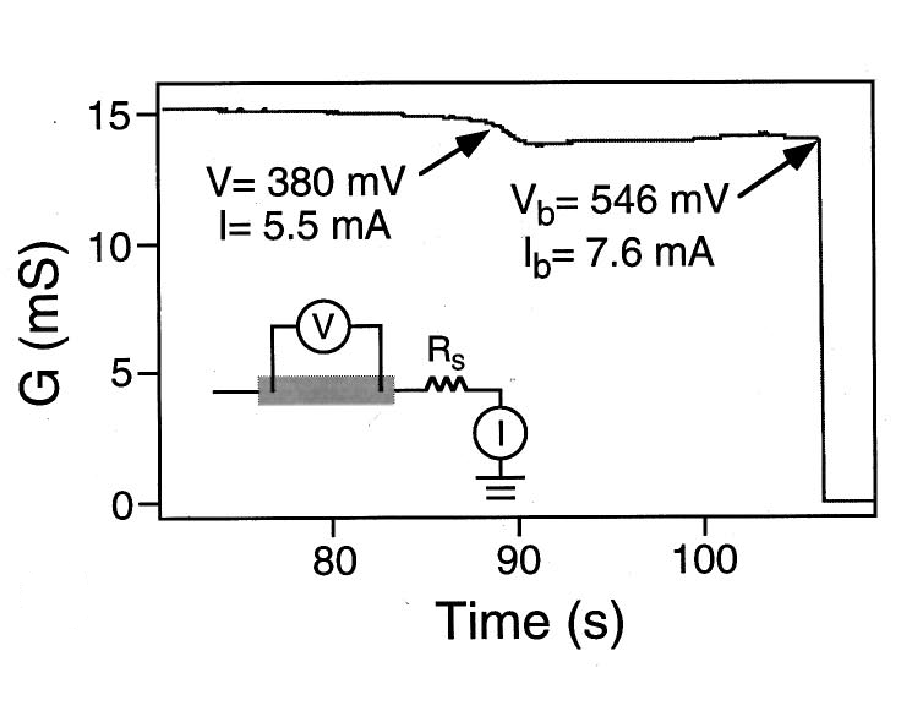
\includegraphics[scale=0.45]{Fabrication/ElecMigExemp/ParkFig.pdf} 
}
\parbox{6.5cm}{\caption{Evolution de la conductance d'un nanofil au court du temps lors d'une procédure d'électromigration à rampe unique. Extrait de~\cite{Park1999}.}
\label{ParkExemp}
}
\end{figure}



\subsubsection{À contre-réaction}
Cette méthode à été développée par Strachan \textit{et al.} en 2005~\cite{Strachan2005}. Elle a pour but de réduire le chauffage de la jonction par effet Joule~\cite{Esen2005} en introduisant une boucle de contre-réaction asservie sur la résistance de la jonction. Si celle-ci dépasse une valeur critique fixée à l'avance, la tension est diminuée puis augmente à nouveau. Ceci à pour effet de réduire la puissance dissipée par la jonction lors de l'électromigration (voir Fig.\ref{EseExemp}). Le principal inconvénient de cette technique est son temps de mise en œuvre : la formation d'un seul gap peu prendre plusieurs heures.


\begin{figure}
\parbox{7cm}{
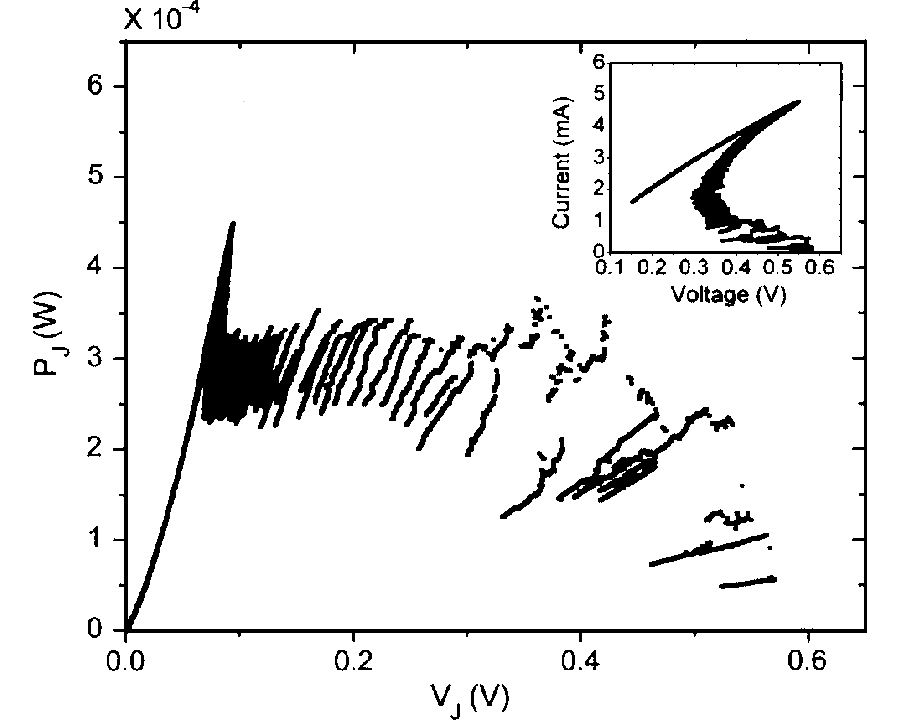
\includegraphics[scale=0.45]{Fabrication/ElecMigExemp/EseFig.pdf} 
}
\parbox{6.5cm}{\caption{Evolution de la puissance dissipée en fonction de la tension appliquée, lors d'une procédure d'électromigration à contre-réaction. En encart, caractéristique courant-tension lors de cette m\^eme procédure. Extrait de~\cite{Esen2005}.}
\label{EseExemp}
}
\end{figure}


\subsubsection{À cassure spontanée}

\begin{figure}
\parbox{7cm}{
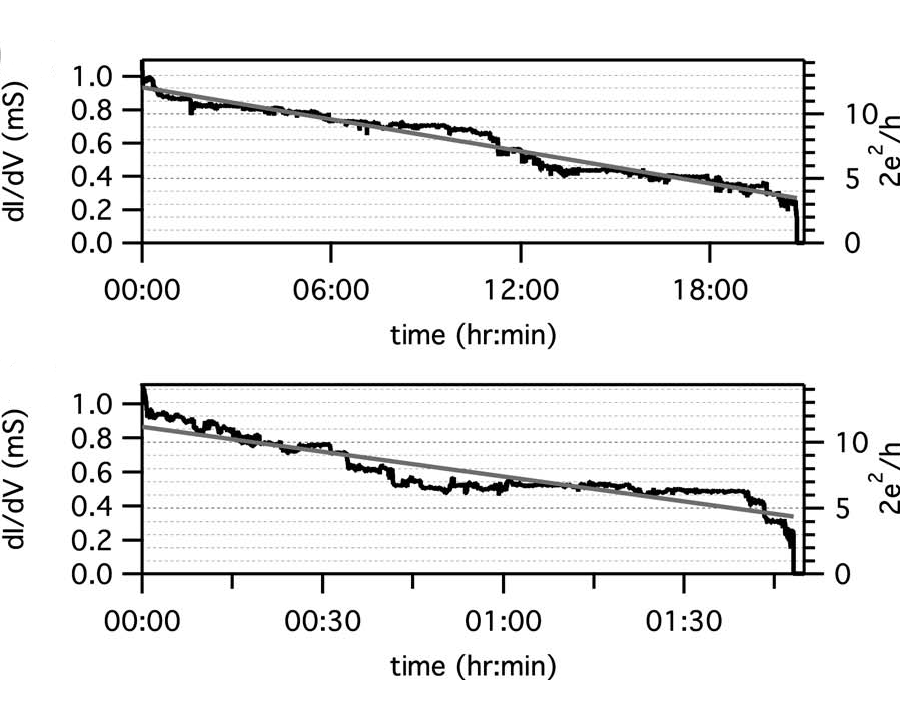
\includegraphics[scale=0.45]{Fabrication/ElecMigExemp/ZantFig.pdf} 
}
\parbox{6.5cm}{\caption{Évolution de la conductance de deux nanofils au cours du temps lors d'une procédure d'électromigration à cassure spontanée. Extrait de~\cite{ONeill2007}.}
\label{ZantExemp}
}
\end{figure}
Cette dernière méthode a été mise au point dans le groupe de H.S.J. van der Zant en 2007~\cite{ONeill2007}. Une première étape d'électromigration contrôlée est d'abord réalisée à l'aide d'une méthode à contre-réaction jusqu'à ce que la conductance du nanofil atteigne une valeur de quelques kilo-Ohms. On laisse ensuite évoluer la jonction qui, du fait de l'instabilité de la nanoconstriction, va se rompre naturellement. On obtient ainsi un gap de quelques nanomètres. La durée d'une telle procédure varie d'un échantillon à l'autres : de quelques minutes à plusieurs heures (voir Fig.\ref{ZantExemp}).


\subsection{Notre technique}


\begin{figure}
\centering 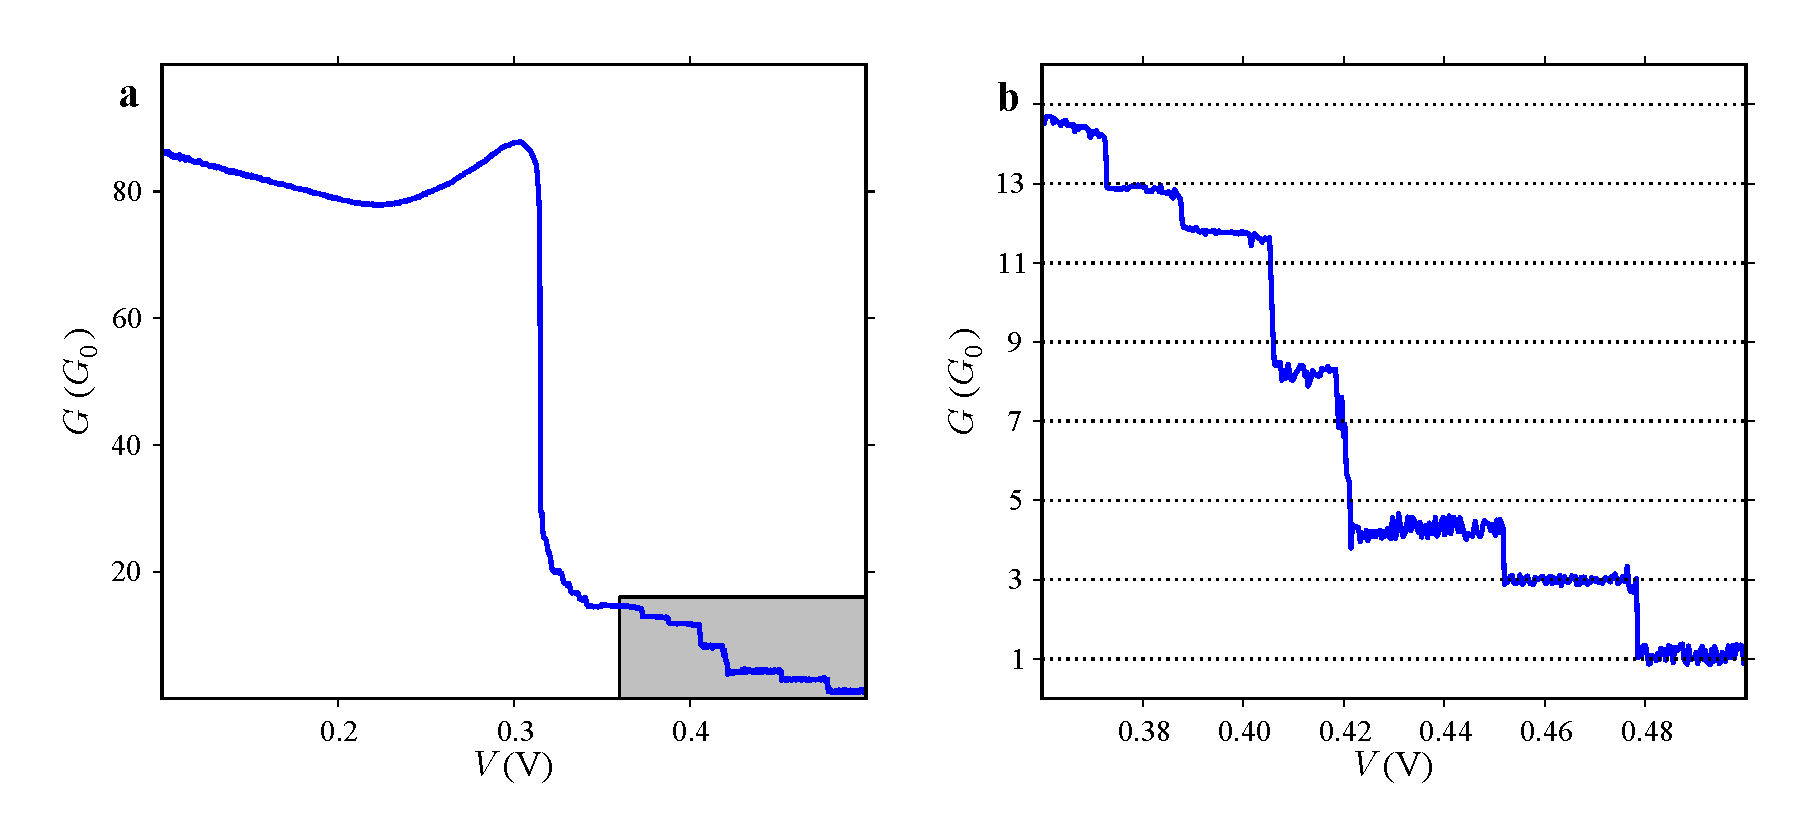
\includegraphics[scale=0.45]{Fabrication/NotreElectroMig/NotreElectroMig.pdf}
\caption{\textbf{a} : conductance de la jonction durant l'électromigration. \textbf{b} : grossissement de la partie grisée de \textbf{a} montrant les marches de conductance témoignant du bon déroulement de l'électromigration.}
\label{NotreElecMig}
\end{figure}

Notre technique de fabrication a été développée à partir des travaux de Park \textit{et al.}~\cite{Park1999} puis améliorée en s'inspirant de travaux ultérieurs.
Afin d'augmenter le rendement de la méthode et la qualité des interstices obtenus, il a fallu apporter quelques modifications. De plus, celle-ci étant réalisée dans un frigo à dilution, il a fallu adapter la procédure à l'impédance des lignes, induite par les différents étages de filtration, en essayant de conserver celle-ci aussi basse que possible~(150\,$\Omega$). En effet, une faible impédance permet de limiter la puissance dissipée au niveau de la jonction et donc de mieux contrôler l'électromigration~\cite{Zant2006,Trouwborst2006,Taychatanapat2007}.

La présence de cette impédence nous impose de contrôler parfaitement le déroulement de l'électromigration. Pour cela, il faut être capable d'agir sur cette dernière en un intervalle de temps similaire à l'échelle de temps du phénomène : du domaine de la centaine de $\mu s$~\cite{ONeill2007}. Ceci n'est possible que si la procédure d'électromigration se fait à l'aide d'une électronique en temps réel. Nous avons pour cela utilisé un ADWin contrôlé par le programme NanoQT, développé au sein du groupe. Grâce à ce dispositif, l'électromigration peut être détectée et la tension aux bornes de la jonction ramenée à zéro dans un intervalle de $10\, \mu s$. Ainsi, nous pouvons obtenir des interstices de la taille souhaitée ($\sim 1\,nm$) de façon reproductible. 



\begin{figure}
\parbox{7cm}{
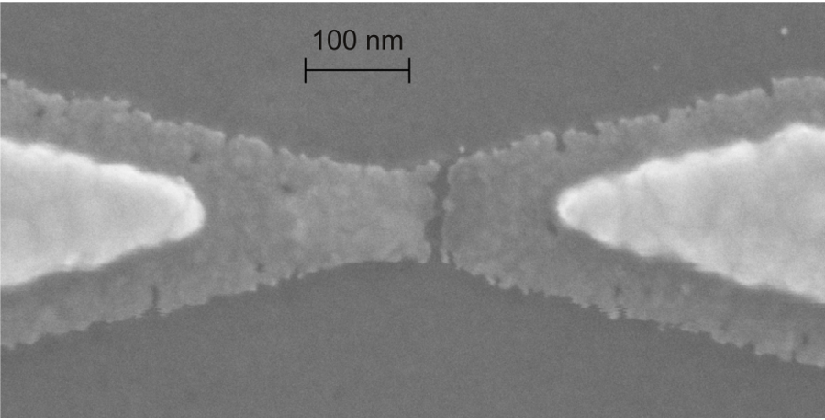
\includegraphics[scale=0.45]{Fabrication/JonctionElecromig/JonctionElecromig.pdf} 
}
\parbox{5cm}{\caption{Image obtenue par microscopie électronique à balayage d'une jonction électromigrée pour laquelle l'interstice nanométrique est clairement visible.}
}
\end{figure}


La Fig.\ref{NotreElecMig} présente la mesure en conductance lors d'un procédure d'électromigration. On observe trois régimes : dans un premier temps, la conductance diminue du fait de l'effet Joule; puis celle-ci augmente à nouveau du fait d'un réarangement de la jonction; enfin, la conductance chute brutalement et le phénomène d'électromigration commence. On peut notamment observer, en fin de procédure, une quantification de la conductance matérialisée par des plateaux, démontrant que l'électromigration est parfaitement contrôlée.

De plus, l'étape d'électromigration se fait à $4\,K$ et sous atmosphère hélium ce qui prévient la contamination de l'interstice et permet d'analyser le dispositif obtenu directement après la procédure.

\section{Fabrication d'un transistor à molécule unique}
Les étapes que nous avons présentées jusqu'à maintenant permettent d'obtenir une structure à trois terminaux~(source, drain et grille). Il nous faut maintenant disposer une molécule unique dans cette structure afin d'obtenir un transistor moléculaire. Pour cela, nous verrons tout d'abord comment les molécules sont déposées avant électromigration. Cette dernière étant effectuée à $4\,K$, elle autorise une caractérisation électrique immédiatement après. Nous détaillerons cette dernière afin de voir quels indices trahissent la présence d'un objet dans l'interstice nanométrique.

Les cristaux de TbPc$_{2}$ sont dissous dans du dichlorométhane à la concentration 10$^{-6}mol.L^{-1}$. La solution obtenue est soumise à un bain d'ultrason afin de prévenir la formation de grappes. La présence de ces dernières pourrait interférer avec l'électromigration, empêchant les molécules de se faire piéger dans l'interstice. Une goutte de la solution obtenue est ensuite déposée sur l'échantillon et séchée par un flux d'azote. L'échantillon obtenu est ensuite microsoudé sur le porte échantillon, disposé dans un frigo à dilution et électromigré à une température de  $4\,K$. Les jonctions obtenues (jusqu'à 12 par échantillons) sont ensuite analysées en transport.

Une fois la jonction électromigrée, il faut s'assurer que l'interstice obtenue contienne un objet. La première analyse généralement effectuée consiste à mesurer la conductance du système en fonction de la tension de grille, pour une tension source-drain nulle. La présence d'un objet nanométrique fait apparaître un ou plusieurs pics, que l'on nomme pics de Coulomb~\cite{Beenakker1991,Wiel2002,Hanson2007}~(cf annexe sur le transport mésoscopique). 

Mais il faut aussi s'intéresser à la nature de l'objet piégé et s'assurer qu'il s'agit bien de la molécule déposée. C'est une question cruciale dans le domaine de l'électronique moléculaire, et en particulier lorsque l'on utilise la technique d'électromigration. En effet, de nombreuses configurations peuvent donner une signature en transport plus ou moins similaire. Une boite quantique peut \^etre formée par une bille d'or crée lors de l'électromigration, par un élement polluant introduit lors de la fabrication ou du dép\^ot des molécules, ou bien encore par la molécule que l'on chercher à étudier. C'est à ce dernier cas que l'on souhaite s'intéresser.

Dans notre cas, nous connaissons la signature magnétique de la molécule que nous souhaitons étudier. Cela facilite considérablement l'interprétation de la mesure. Nous n'avons qu'à analyser les propriétés magnétiques de l'objet piégé au sein de l'interstice, pour en déduire la nature et la configuration en transport. La méthode utilisée sera détaillée dans le chapitre suivant, consacré aux résultats expérimentaux.  S'il s'avère que la molécule est bien responsable du transport électronique, alors nous avons obtenu un transistor moléculaire tel que celui décrit dans la Fig.\ref{ImageTrans}.



%\chapter{Résultats expérimentaux}

\section{L'aimant moléculaire TbPc$_{\rm{2}}$}
Nous avons vu dans le chapitre premier qu'un aimant moléculaire était, en général, composé de plusieurs centres magnétiques interagissant entre eux, et que, de cette interaction, résultait un moment magnétique. Le terbium double-decker, nommé ainsi par analogie aux biplans de la première guerre mondiale, n’obéit pas à cette description. En effet, il comporte un unique centre magnétique, l'ion terbium, pris en sandwich entre deux ligands, les phtalocyanines (cf Fig.\ref{TbPc2Imag}). Il présente néanmoins des propriétés magnétiques similaires aux autres aimants moléculaires à plusieurs centres, avec cependant quelques particularités, que nous détaillerons dans la suite.

\begin{figure}
\centering 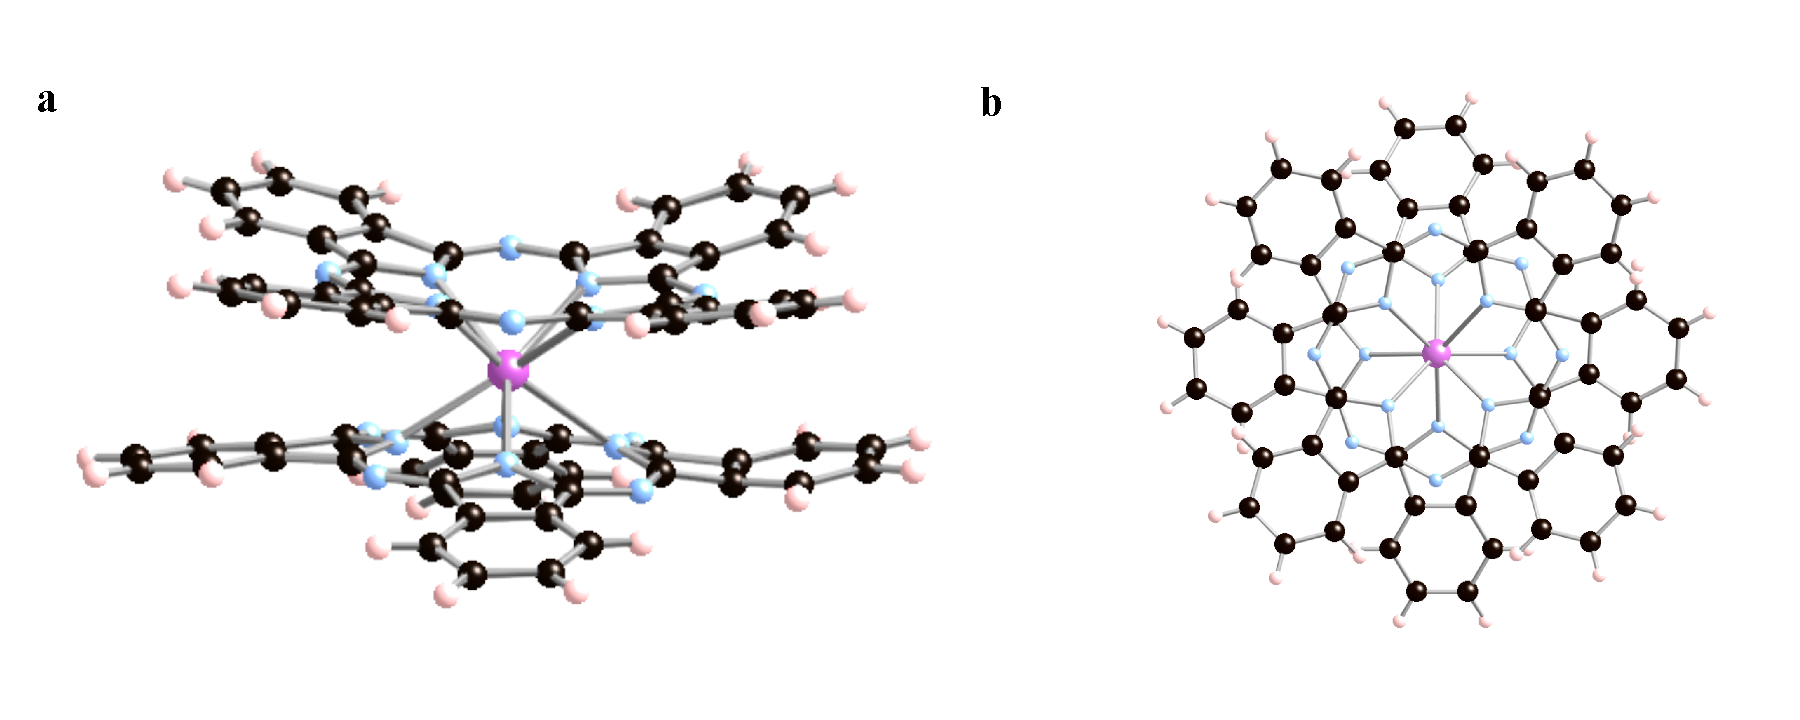
\includegraphics[scale=0.45]{Resultats/TbPc2Imag/TbPc2Imag.pdf} 
\caption{Vue d'artiste de la molécule de terbium double-decker de côté~(\textbf{a}) et de dessus~(\textbf{b}). L'atome de terbium, ici en violet, est pris en sandwich entre deux phtalocyanines, ces derniers étant orientés à $45\degres$ environ, l'un par rapport à l'autre. Les atomes d'azote et de carbone sont représentés respectivement en bleu et noir.}
\label{TbPc2Imag}
\end{figure}





\subsection{Origine du moment magnétique}
Le moment magnétique du terbium double-decker est d\^u à un centre magnétique unique : l'ion Tb$^{3+}$. L'atome de terbium appartient à la classe des lanthanides. Son magnétisme est porté par la couche $4f$ et résulte d'un fort couplage entre le moment de spin et le moment orbital. Le moment magnétique total de l'état fondamental $J=6$ est issue, à contribution égale, du moment magnétique orbital $L=3$, et des moments magnétiques de spin des 6 électrons non appariés $S=3$. Le premier état excité $J=5$ est distant de $2900\,K$, et peut donc \^etre ignoré lorsque l'on s'intéresse aux propriétés magnétiques de l'ion Tb$^{3+}$.
 

\begin{figure}
\centering 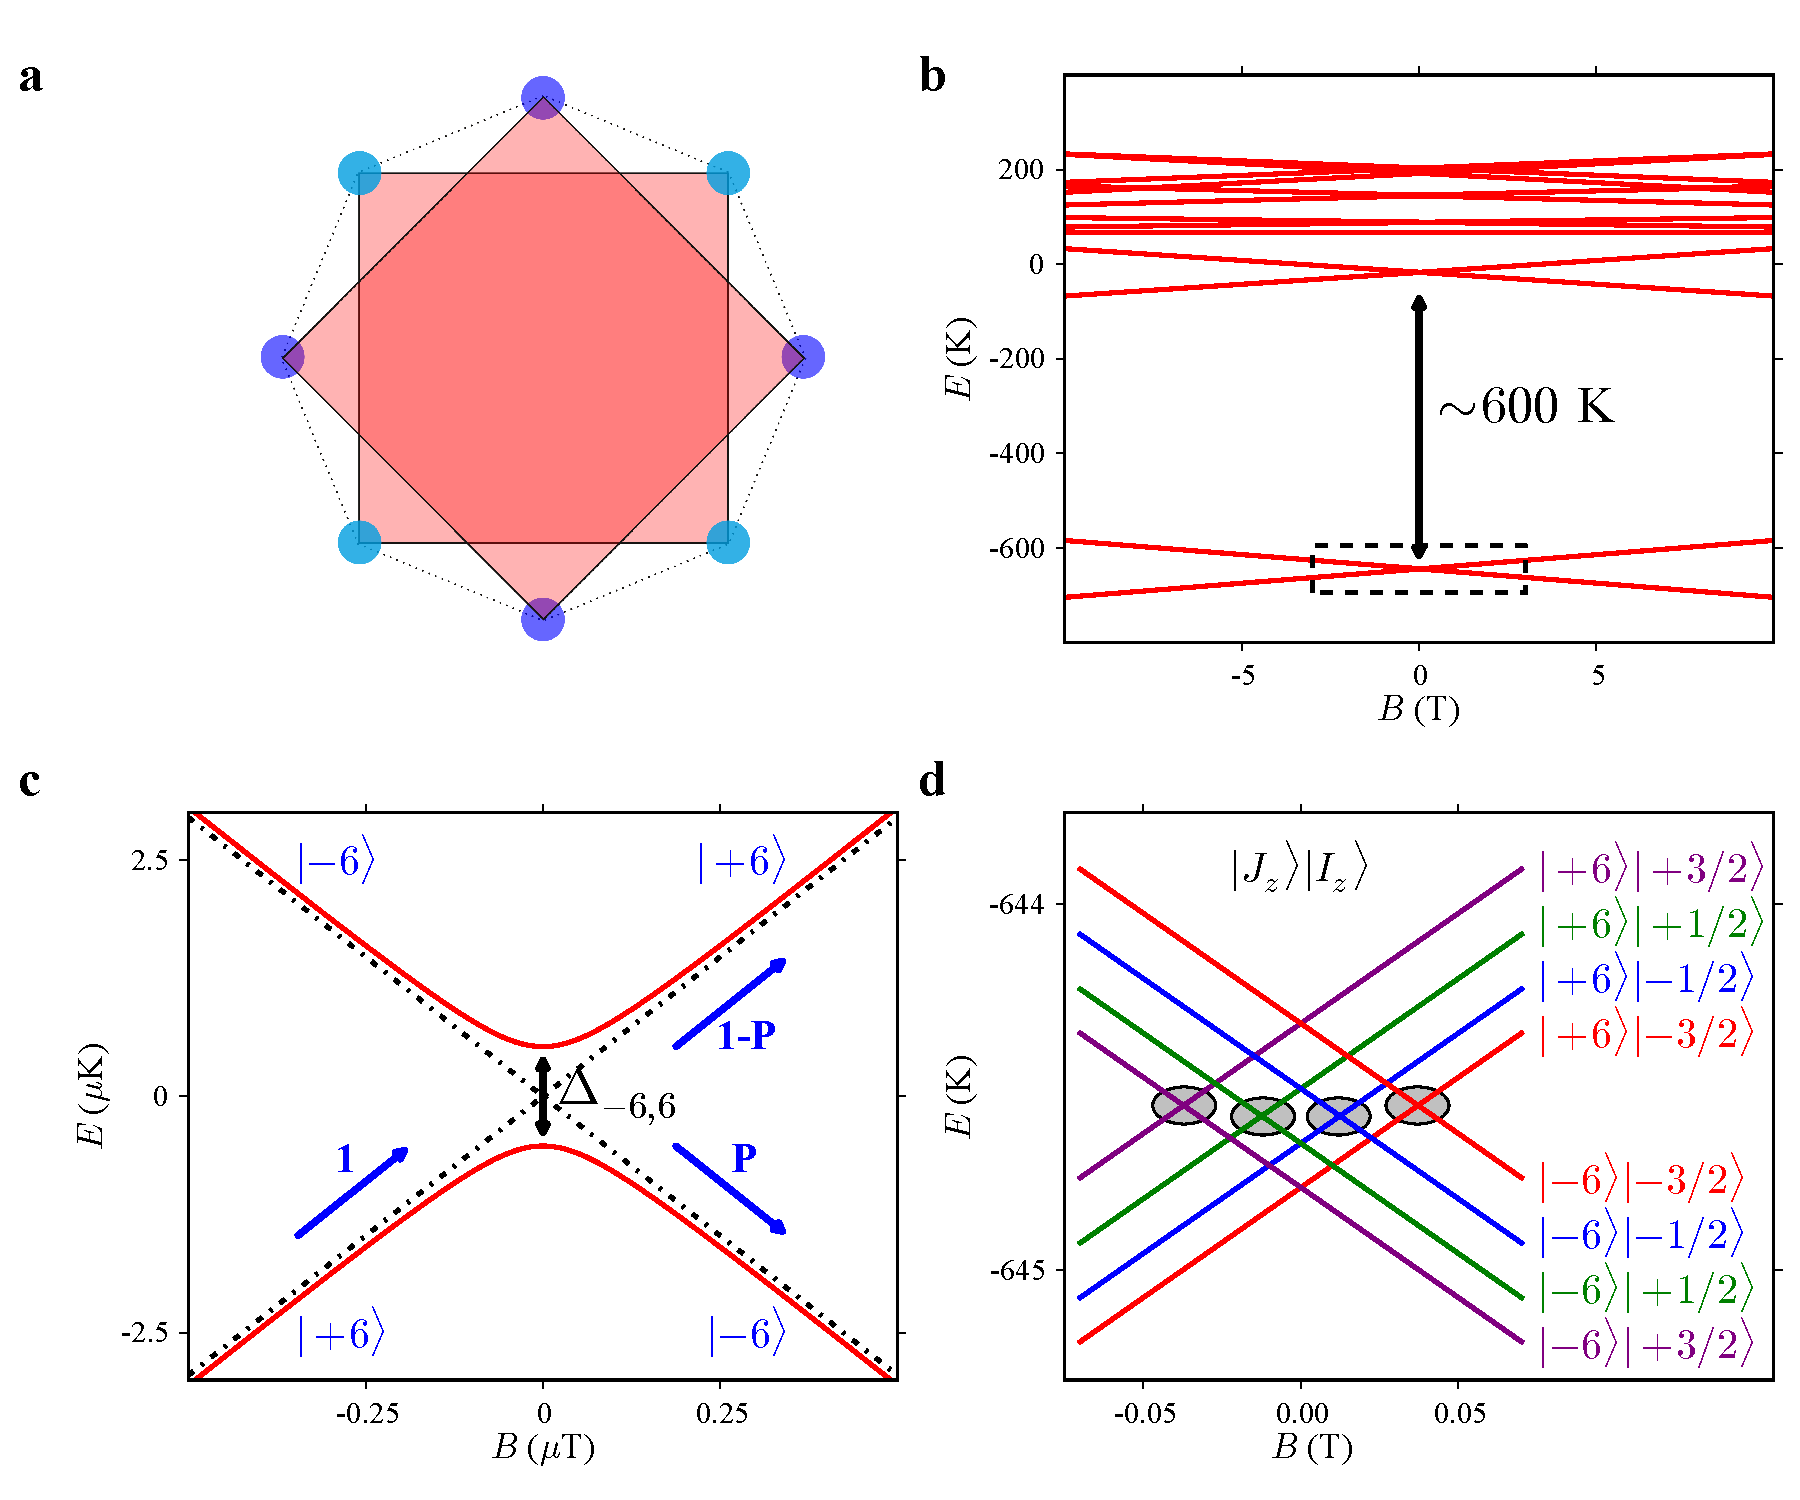
\includegraphics[scale=0.45]{Resultats/TbPc2Mag/TbPc2Mag.pdf} 
\caption{\textbf{a} : schémas représentant la coordination anti-prisme. Les atomes d'azote sont représentés en bleu clair et bleu foncé, chaque couleur correspondant à un plan de ligand. \textbf{b} : diagramme Zeeman de la molécule TbPc$_2$ représentant l'énergie des différents états du système en fonction du champ magnétique. Les états fondamentaux $J_z \pm 6$ sont séparés des premiers états excités par une énergie de $600$\,K. \textbf{c} : agrandissement du diagramme Zeeman des deux états fondamentaux à faible champ magnétique. Il met en évidence un anti-croisement de valeur minimale $\Delta_{-6,6}$ de l'ordre du $\mu$K qui traduit un mélange entre les états $|+6\rangle$ et $|-6\rangle$. Si l'on balaie le champ magnétique des valeurs négatives vers les valeur positives, il existe une probabilité $P$ de passer de l'état $|+6\rangle$ à l'état $|-6\rangle$. Cette probabilité est régie par la formule de Landau-Zenner. \textbf{d} : Diagramme Zeeman lorsque l'on tient compte du couplage hyperfin entre le spin $I=3/2$ du noyau et le moment magnétique électronique. Les deux doublets sont séparés en deux jeux de quatre sous-états. On ne relève que quatre anti-croisements marqués d'un cercle, où une transition de l'état  $|+6\rangle$ à l'état $|-6\rangle$ est possible.~(inspiré de \cite{Ishikawa2005} et \cite{Sorace2011}).}
\label{TbPc2Zeeman}
\end{figure}


\subsection{Hamiltonien}

Si l'on veut maintenant décrire le diagramme énergétique de la molécule aimant TbPc$_{2}$, deux contributions majeures doivent être prises : l'influence des ligands et le couplage hyperfin entre le moment magnétique électronique du terbium et son spin nucléaire.

\subsubsection{Le moment magnétique électronique}
Le moment magnétique de l'ion terbium est soumis à un champ de ligand définie principalement par la longueur des liaisons covalentes et la symétrie du système. 
L'ion terbium est lié de façon covalente à huit atomes d'azote, quatre pour chaque phatlocyanide~(cf Fig.\ref{TbPc2Imag}). La géométrie des deux ligands, orientés à $45\degres$ l'un par rapport à l'autre, selon un axe perpendiculaire au plan des ligands, correspond à une coordination dite anti-prisme~(cf Fig.\ref{TbPc2Zeeman}.\textbf{a}). 

On peut rendre compte de cette coordination à l'aide des opérateurs de Stevens $O_2^0$, $O_4^0$ et $O_6^0$~\cite{Stevens1952,Sorace2011}. On obtient alors l'expression suivante :
\begin{eqnarray}
H = \alpha A_2^0 \langle r^2 \rangle O_2^0 + \beta A_4^0 \langle r^4 \rangle O_4^0 + \gamma A_6^0 \langle r^6 \rangle O_6^0
\end{eqnarray}
où $A_i^0$ sont les coefficients relatifs à la molécule de TbPc$_2$~\cite{Ishikawa2005} et $\alpha$, $\beta$ et $\gamma$ les coefficients introduits par Stevens~\cite{Stevens1952}. Les opérateurs $O^0_i$ sont basés sur des sommes d'opérateurs $S_z^{2n}$. La symétrie du système n'introduit pas de couplage entre les différents états magnétiques. 

Ainsi, en prenant en compte les éléments que l'on vient d'introduire, on obtient le diagramme Zeeman présenté dans la Fig.\ref{TbPc2Zeeman}.\textbf{b}. Les états fondamentaux $J_z = \pm 6$ sont isolés des états excités par une énergie de plus de $600\,K$. Cela garantie, à basse température, deux états possibles pour le système : $J_z = \pm 6$. Dans la suite de notre description, on pourra négliger les états excités.

 
Cependant, du fait des interactions $\pi - \pi$ entre ligands, l'angle entre les deux plans n'est pas exactement égal à $45\degres$~\cite{Koike1996}. Cela entraîne une brisure de symétrie, et nécessite l'introduction d'un nouveau terme dit terme transverse~\cite{Sorace2011} :
\begin{eqnarray}
H_{trans} = \beta A_4^4 \langle r^4 \rangle O_4^4
\end{eqnarray}
où la m\^eme notation a été utilisée. Ce dernier terme ne modifie pas l'allure générale du diagramme Zeeman. En revanche, il introduit un couplage entre les états  $J_z = \pm 6$ qui se traduit par la présence d'anti-croisement que nous allons détailler maintenant.

\subsubsection{Les anti-croisements}
La Fig.\ref{TbPc2Zeeman}.\textbf{c} présente un grossissement du diagramme Zeeman au niveau de l'anti-croisement repéré par le carré de la Fig.\ref{TbPc2Imag}.\textbf{b}. Les lignes en pointillées correspondent au diagramme Zeeman en l'absence de terme transverse. Si l'on se place loin de l'anti-croisement, les états $|+6\rangle$ et $|-6\rangle$ sont les états propres du système. Mais plus on se rapproche de l'anti-croisement, plus les états se mélangent.

Lorsque l'on balaie le champ magnétique autour d'un anti-croisement, il existe une probabilité de passer de l'état $|+6\rangle$ à l'état $|-6\rangle$ et vice-versa. Cette probabilité est régie par la formule de Landau-Zener~\cite{Zener1932} qui dépend à la fois de la séparation minimale entre les deux niveaux~$\Delta_{-6,6}$, ainsi que de la vitesse de balayage du champ magnétique~$\frac{dB_z}{dt}$. Cette probabilité peut s'exprimer de la façon suivante :
\begin{eqnarray}
P = 1 - \exp \left( -\frac{\pi \Delta^2_{m,m'}}{2 \hbar g \mu_B |m-m'|\frac{dB_z}{dt}} \right)
\label{LandauZener}
\end{eqnarray}
ou $P$ est la probabilité de passer de l'état $m$ à l'état $m'$, $m$ et $m'$ valant dans notre cas, respectivement $+6$ et $-6$. Si la vitesse est très faible, la probabilité de passer d'un état à l'autre tend vers un. On retrouve ici le théorème adiabatique. A l'autre bout de l'échelle, si le champ magnétique est balayé très rapidement, cette probabilité tend vers zéro. Tout se passe comme si le système n'avait pas eu le temps de ``sentir" l'anti-croisement.




\subsubsection{Le spin nucléaire}
De part leur forme, les orbitales $4f$ impliquées dans le magnétisme du terbium favorisent le couplage hyperfin. Il est donc possible de mesurer l'influence de ce dernier sur les propriétés magnétiques de la molécule TbPc$_{2}$. Le spin nucléaire du terbium étant $I = 3/2$, on obtient en lieu et place des deux niveaux fondamentaux $J_z \pm 6$, deux jeux de quatre niveaux comme le montre la Fig.\ref{TbPc2Zeeman}.\textbf{d}. Cette interaction peut être prise en compte en introduisant le terme suivant dans l'hamiltonien~\cite{Bleaney1961} :
\begin{eqnarray}
H_{hf} = A_{hf}\mathbf{J}\mathbf{I}
\end{eqnarray}
où $\mathbf{J}$ et $\mathbf{I}$ sont respectivement le moment magnétique électronique et le spin nucléaire, $A_{hf}$ étant la constante d'interaction hyperfine. Il est important de noter que le terbium ne possède qu'un seul isotope, et donc un seul spin nucléaire possible.

Du fait de sa forme allongée, le spin nucléaire possède également un moment quadripolaire dont on peut tenir compte par le terme suivant~\cite{Bleaney1961} :
\begin{eqnarray}
H_I = P\left(I_z^2 - \frac{1}{3}I(I+1)\right)
\end{eqnarray}
où $P$ est le moment quadripolaire du spin nucléaire. La présence de ce terme a pour conséquence de rendre l'espacement entre les différents niveaux non-uniforme. Ceci peut notamment avoir des applications dans le cadre de l'information quantique~\cite{Leuenberger2003}. Nous détaillerons ce dernier point plus tard, lorsque nous évoquerons les possibilités de manipulation du spin nucléaire dans le dernier chapitre.

Un diagramme Zeeman incluant l'ensemble de ces contributions est présenté dans la Fig.\ref{TbPc2Zeeman}.\textbf{d}, pour les faibles champs magnétiques~(de -70 à 70$\,mT$).



\subsection{Mesure de l'aimantation d'une assemblée}
Afin d'explorer les propriétés magnétiques des aimants moléculaires, plusieurs techniques sont envisageables. De manière générale, il faut tout d'abord obtenir un cristal moléculaire constitué par l'aimant moléculaire que l'on souhaite étudier. L'aimantation du cristal est ensuite mesurée en fonction du champ magnétique appliqué. Pour cela, on peut utiliser, par exemple, la technique du micro-SQUID, qui a l'avantage d'autoriser les mesures sub-kelvins. Il s'agit d'un détecteur de variation de flux basé sur deux jonctions Josephson, dont la sensibilité est de l'ordre de $500\, \mu_B$.

Lorsque l'on mesure un cristal moléculaire, la variation d'aimantation moyenne, induite par le retournement du moment magnétique des molécules qui le composent, entraîne une modification du flux traversant le micro-SQUID, qui peut être mesurée. A partir de cette mesure, et en considérant chaque aimant moléculaire comme isolé, on peut remonter aux propriétés magnétiques de ces derniers.

\begin{figure}
\centering 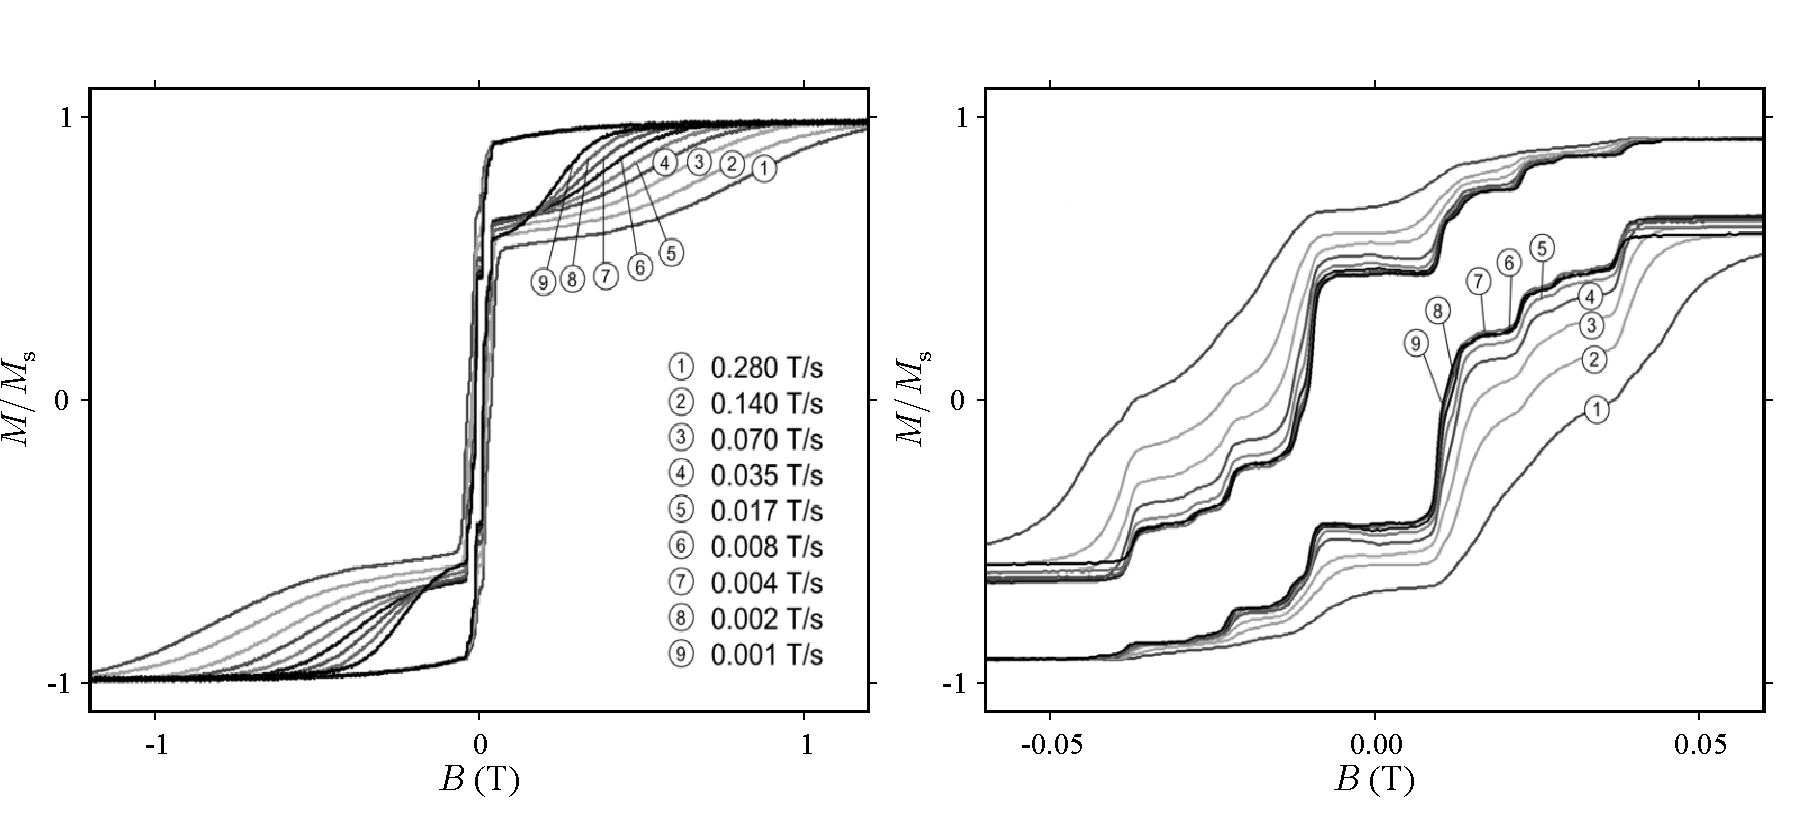
\includegraphics[scale=0.45]{Resultats/MesureAimant/MesureAimant.pdf} 
\caption{\textbf{a} : Mesure de l'aimantation d'un cristal de TbPc$_2$ dilués à 10\,\% pour différentes vitesses de balayage. \textbf{b} : grossissement de la partie centrale mettant en évidence l'influence de la vitesse de balayage sur la hauteur des marches associées au retournement par QTM.(extrait de \cite{Ishikawa2005}).}
\label{TbPc2Aimantation}
\end{figure}


Une mesure de l'aimantation d'un cristal de TbPc$_2$ pour différentes vitesses de balayage est présentée dans la Fig.\ref{TbPc2Aimantation}.\textbf{a}. Une analyse détaillée peut \^etre trouvée dans \cite{Ishikawa2005}. On peut diviser la courbe en deux zones. 

A faible champ~(cf Fig.\ref{TbPc2Aimantation}.\textbf{b}), les molécules constituant le cristal se retournent par QTM. Les marches rendent compte du retournement de l'aimantation au niveau des anti-croisements présentés dans la Fig.\ref{TbPc2Zeeman}.\textbf{d}. Cependant, le nombre de transitions est supérieur aux quatre prédites par la théorie. Les transitions supplémentaires résultent de l'interaction entre les différentes molécules aimants constitutives du cristal moléculaire. Comme le montre l'Equ.\ref{LandauZener}, le probabilité de transition est fonction de la vitesse de balayage, ce qui conduit à une variation de la hauteur des marches en fonction de celle-ci, mise en évidence par mesure de la Fig.\ref{TbPc2Aimantation}.\textbf{b}. 

A plus fort champ, l'aimantation ne peut se retourner qu'en émettant un phonon. La position en champ magnétique de ces retournements directs dépend donc de la distribution en énergie des phonons du système, d'où la zone de transition continue.

\subsection{TbPc$_2$ et la spintronique}
Pour qu'un aimant moléculaire puisse être utilisé dans le cadre de la spintronique moléculaire, il doit remplir plusieurs critères : il doit conserver ses propriétés magnétiques lorsqu'il est déposé sur une surface métallique; il doit également être relativement robuste vis-à-vis de la déformation; enfin, dans le cas de l'électromigration, il doit pouvoir résister à des températures de plusieurs centaines de degrés Celsius.

\begin{figure}
\centering 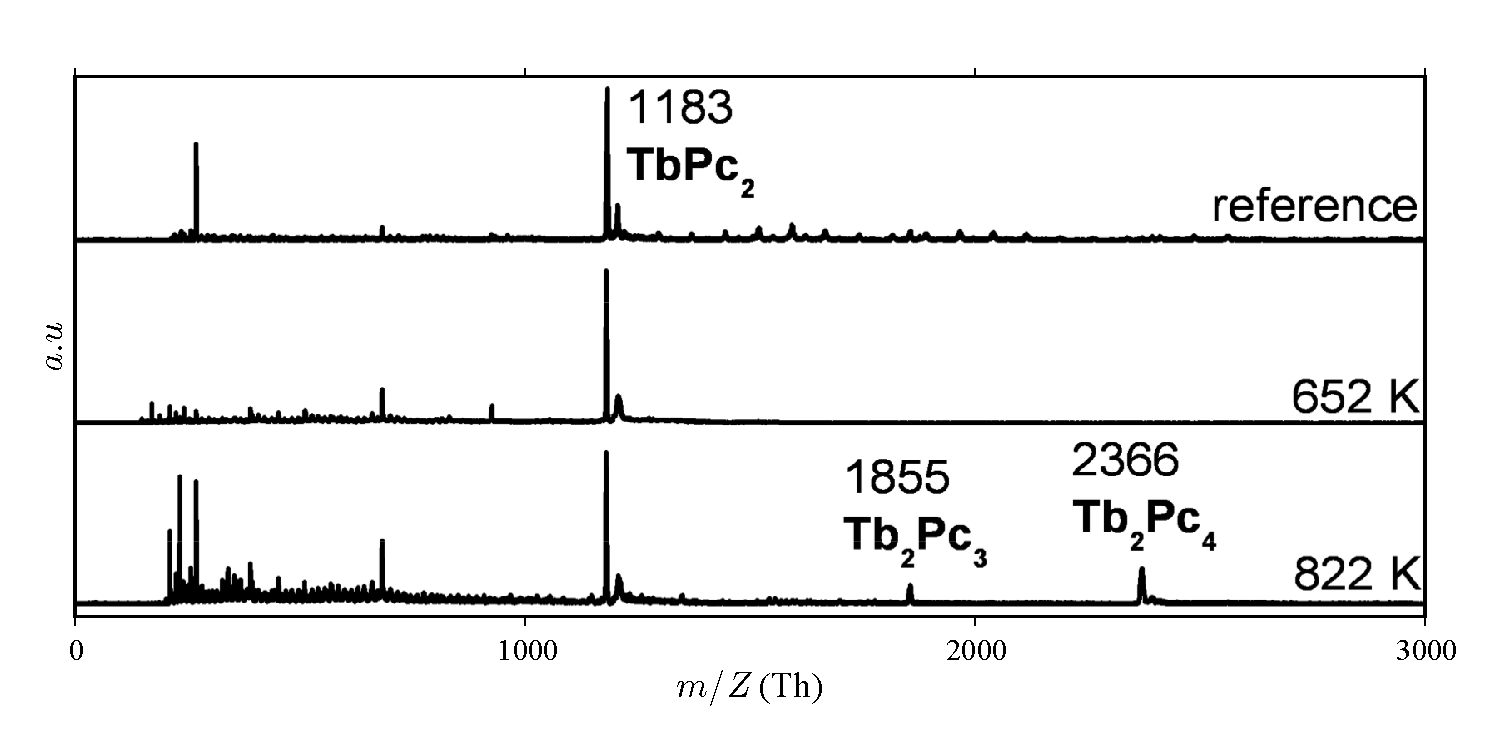
\includegraphics[scale=0.45]{Resultats/TbPcResTemp/TbPcResTemp.pdf} 
\caption{Spectromètre obtenue par évaporation à différente température d'une poudre de TbPc$_2$. Un échantillon de cette même poudre dissoute dans du dichlormethane et de l'ethanol a servi de référence. (extrait de \cite{Stepanow}).}
\label{SpectMass}
\end{figure}

L'analyse des propriétés magnétiques du TbPc$_{2}$ sur des surfaces de cuivre a été étudié par XMCD~(X-ray Magnetic Circular Dichroism). Cette étude a confirmé la robustesse des propriétés magnétiques vis-à-vis de l'adsorption sur une surface conductrice. De plus, la technique de dép\^ot impliquait de chauffer la poudre d'aimant moléculaire à des températures de plusieurs centaines de degrés. Une analyse au spectromètre de masse a montré que la structure du TbPc$_{2}$ pouvait demeurer intacte jusqu'à une température de $820\,K$~(cf Fig.\ref{SpectMass}). En effet, si à cette température des composés de Tb$_2$Pc$_3$ et Tb$_2$Pc$_4$ peuvent se former, la signature du TbPc$_2$ reste clairement visible et majoritaire. Enfin, si elle reste sensible aux déformations en compression, elle se montre en revanche peut dépendante de la déformation en torsion~\cite{Sorace2011}, cette dernière ne venant modifier que légèrement le terme $A_4^4 \langle r^4 \rangle$ dans la description du système~(et donc la probabilité de retournement par QTM).

Cet aimant moléculaire a, en outre, l'avantage de mettre en jeux magnétisme électronique et magnétisme nucléaire, ce qui rend la physique plus riche, et donc les applications éventuelles plus nombreuses. De plus, le terbium ne possède qu'un seul isotope, ce qui garantit les mêmes propriétés magnétiques, quelque soit l'aimant moléculaire.

\section{Magnétisme et transport}
Afin de comprendre comment le magnétisme moléculaire peut se coupler au transport électronique, il est nécessaire d'identifier les mécanismes régissant ce dernier, dans le cas de structures nanométriques. La première partie de cette section sera consacrée à cette étude.
Nous décrirons ensuite comment ces mécanismes peuvent \^etre sensibles au moment magnétique d'une molécule unique, à travers deux configurations différentes. Enfin, nous aborderons les différentes interactions permettant de coupler le magnétisme moléculaire et le transport mésoscopique.

\subsection{Transport à travers un point quantique}
Un point quantique peut se définir comme un système de petite taille dans lequel les niveaux d'énergies sont discrets. Lorsque l'on couple un point quantique à deux électrodes conductrices, on obtient la configuration de la Fig.\ref{DotSchem}.\textbf{a}, où des niveaux d'énergie discrets sont séparés du continuum d'état des électrodes par une barrière tunnel définie par les paramètres $\gamma_i$, et le couplage capacitif $C_i$~($i=s$ pour la source et $i=d$ pour le drain).

En appliquant une tension source-drain, on ouvre une fenêtre de potentiel chimique. Si le potentiel chimique du point quantique se situe en dehors de cette fen\^etre, l'état de charge de ce dernier est défini, et aucun courant ne traverse le système~(cf Fig.\ref{DotSchem}.\textbf{a}). En revanche, si ce dernier se trouve dans cette fen\^etre, les électrons peuvent circuler en passant un à un à travers l'\^ilot central, et un courant est alors mesuré~(cf Fig.\ref{DotSchem}.\textbf{b}). 

\begin{figure}
\centering 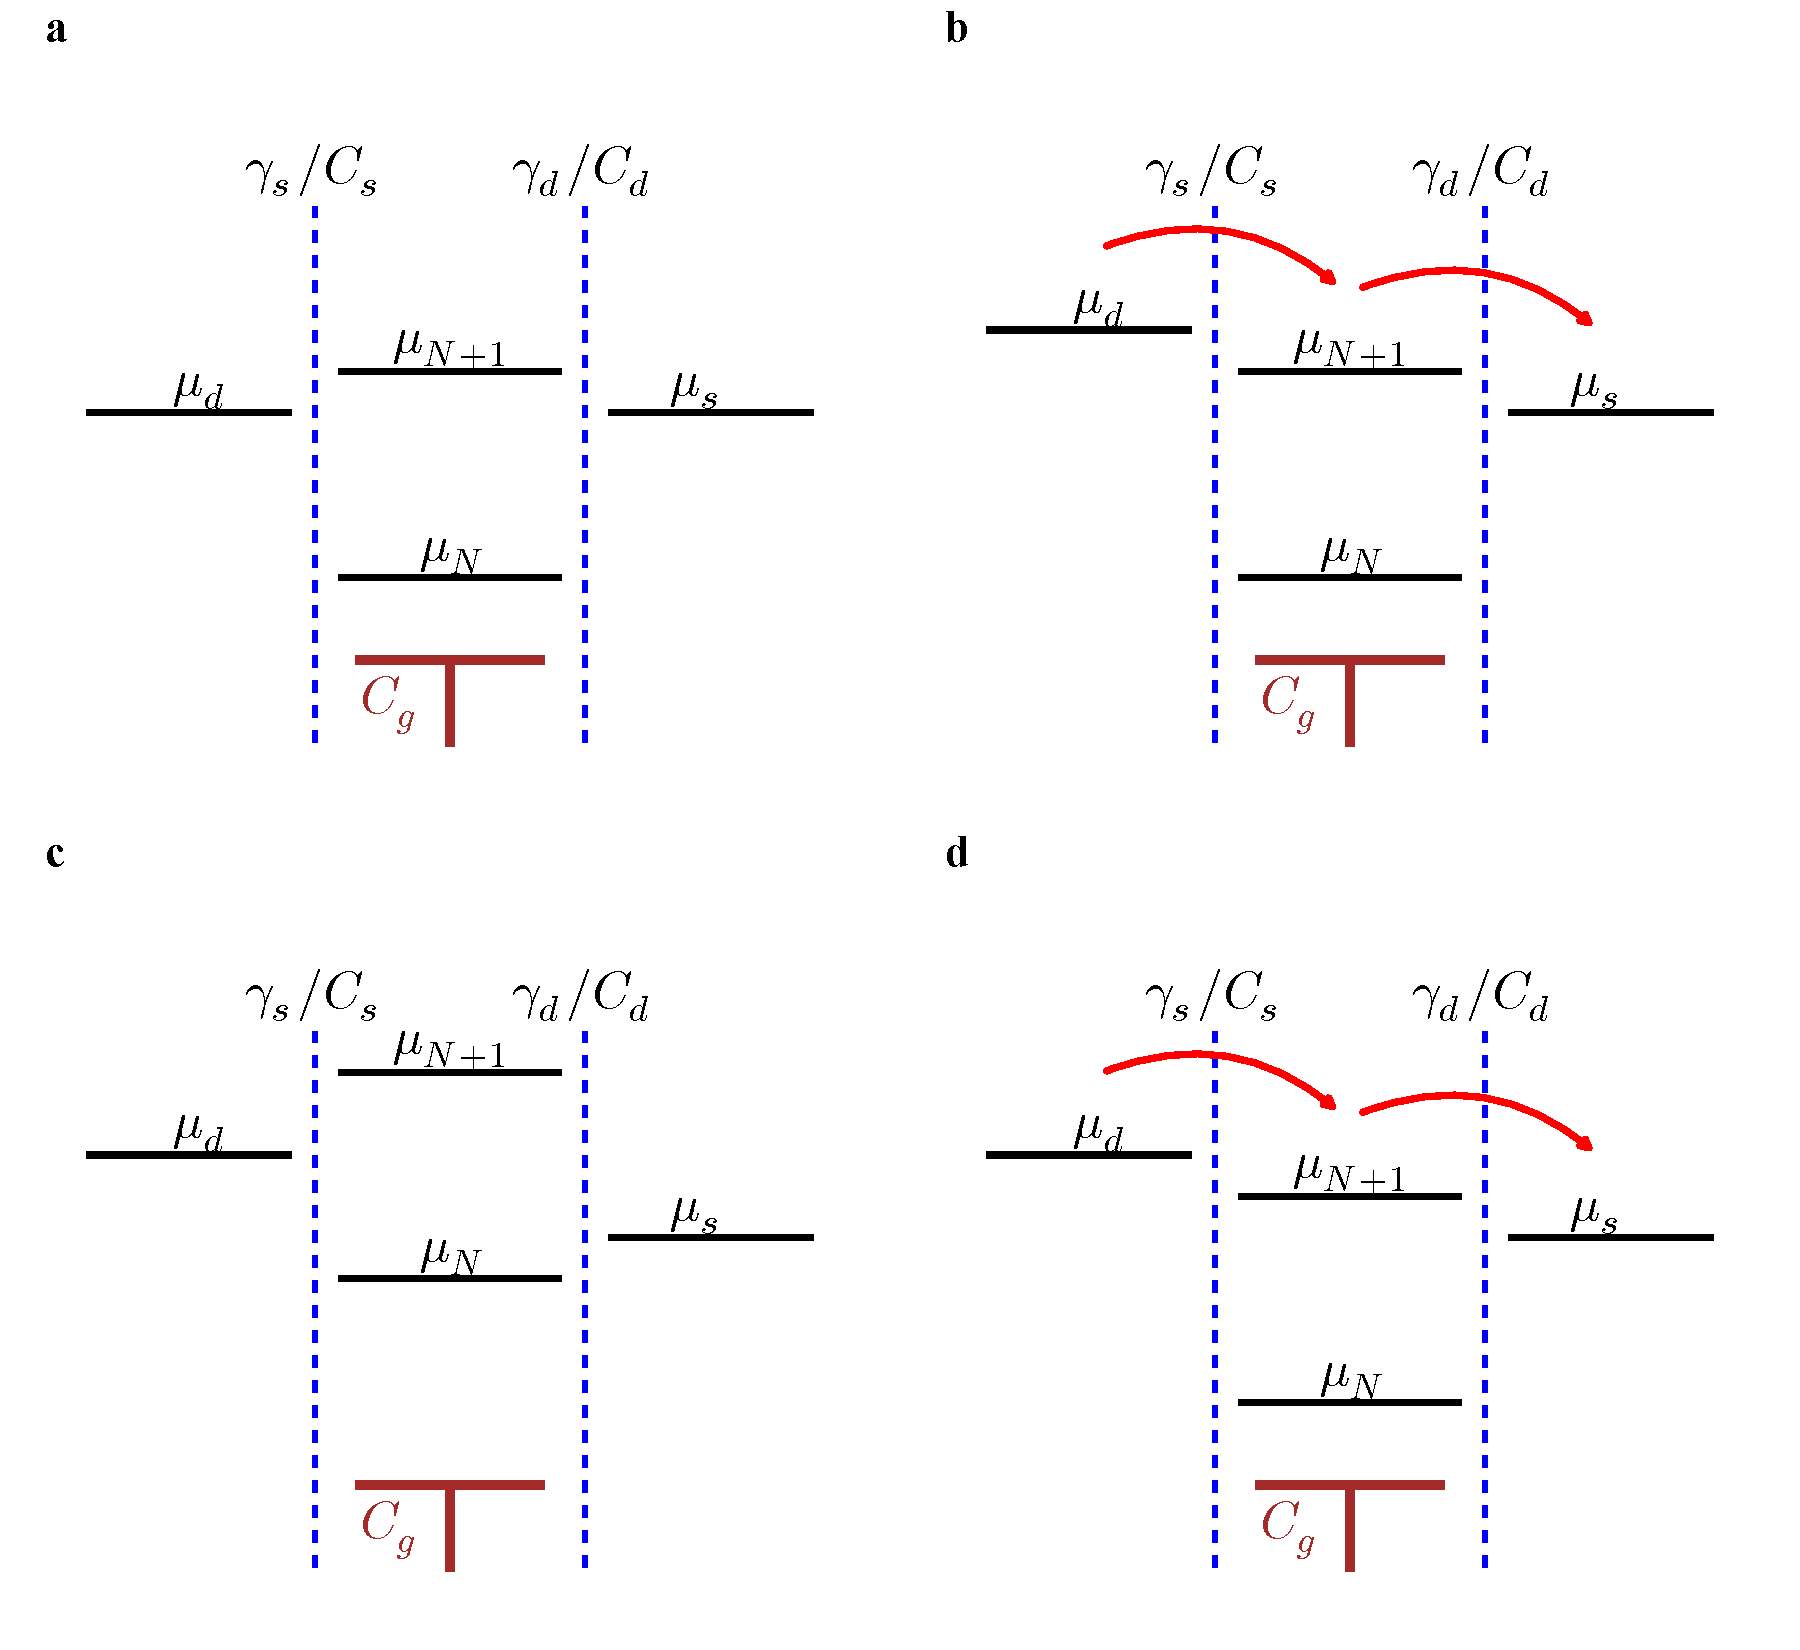
\includegraphics[scale=0.45]{Resultats/DotSchem/DotSchem.pdf} 
\caption{Représentation schématique d'un point quantique. \textbf{a} : Lorsque les potentiels chimique de la source et du drain~($\mu_s$ et $\mu_d$) ne sont pas alignés avec ceux du point quantique, aucun courant ne circule, et l'état de charge du point quantique est bien défini~(ici N). \textbf{b} : en appliquant une tension source drain, on ouvre une fenêtre de potentiel chimique. Si le potentiel chimique du point quantique se trouve dans cette fenêtre, un courant peut circuler. De plus, en appliquant une tension sur l'électrode de grille, on peut amener un potentiel chimique du point quantique, initialement en dehors de la fenêtre~(\textbf{c}), à l'intérieur de celle-ci~(\textbf{d}), induisant un courant.}
\label{DotSchem}
\end{figure}


Afin de pouvoir moduler le potentiel chimique du point quantique, on peut ajouter une électrode de grille. En appliquant une tension sur cette électrode, l'échelle des potentiels chimiques du point quantique peut être décalée, et donc, le courant modulé. On peut ainsi passer d'une situation où le courant est nul~(cf Fig.\ref{DotSchem}.\textbf{c}), à une situation ou les électrons peuvent circuler~(cf Fig.\ref{DotSchem}.\textbf{d}).

On peut maintenant imaginer deux configurations. Dans la première, le point quantique est défini par la centre magnétique, et ce dernier va osciller entre deux états de charge, et donc, deux configurations magnétiques~(cf Fig.\ref{DirVsInd}.\textbf{a}). 
Dans la deuxième configuration, le point quantique n'est pas confondu avec le centre magnétique, mais seulement couplée magnétiquement à ce dernier~(cf Fig.\ref{DirVsInd}.\textbf{b}). Dans la suite, la première configuration sera qualifiée de configuration directe, et la seconde, de configuration indirecte.


\subsection{La configuration directe}
La configuration directe implique que les électrons, responsables du courant, jouent également un rôle dans le magnétisme de la molécule. Cette dernière va osciller entre deux états de charge N/N+1 , chacun d'eux ayant sa propre configuration magnétique $S_N$ et $S_{N+1}$~(cf Fig.\ref{DirVsInd}.\textbf{a}). L'analyse se fait en sondant la différence en énergie des différentes transitions N/N+1~(i.e. la position des potentiels chimiques associés à chaque transition), le plus souvent, par une technique de spectroscopie en tunneling séquentiel~(cf annexe sur le transport mésoscopique). Celle-ci a l'avantage de donner accès à différents états de charge~(nombre d'oxydation ou de réduction). En revanche, le caractère très invasif de la méthode ne laisse pas espérer de long temps de vie pour les différents états du système. Cette dernière a été mise en œuvre expérimentalement dans \cite{Heersche2006,Jo2006,Zyazin2010} avec des résultats mitigés, du fait notamment de la dégradation de la molécule lors de la fabrication du dispositif~\cite{Jo2006}. Des études théoriques ont également été menées~\cite{Timm2006,Timm2007}, permettant une analyse plus fine des résultats expérimentaux.

\subsection{La configuration indirecte}

Dans le cas de la configuration indirecte, les électrons responsables du courant ne participent qu'indirectement au magnétisme de la molécule~(cf Fig.\ref{DirVsInd}.\textbf{b}). Comme nous le montrerons dans la suite, la mesure se fait par l'analyse statistique des modifications de conductance du système en fonction du champ magnétique. La polarisation en tension source-drain et grille est, en général, fixée~(par opposition à la spectroscopie en tunneling séquentiel). Dans cette configuration, le nombre d'électrons impliqués dans le magnétisme moléculaire ne peut pas être modifié. En revanche, la technique de mesure en configuration indirect se révèle beaucoup moins invasive. Cela garantie, d'une part, la préservation des propriétés magnétiques, et d'autre part, l'observation de longs temps de vie des états de spin mesurés. 

Cette configuration a été utilisée dans deux dispositifs différents au sein de notre groupe. Dans le premier, une deuxième molécule~(un nanotube) a été utilisée comme point quantique sonde, l'aimant moléculaire étant déposé sur sa surface \cite{Urdampilleta2011}. Dans le deuxième dispositif, une seule molécule a été utilisée. Le cœur magnétique de cette dernière étant fortement découplé des ligands périphériques, ils ont pu être utilisés comme point quantique sonde~\cite{Vincent2012}. Cette dernière configuration correspond au dispositif que nous nous proposons d'étudier dans la suite. Quelques outils théoriques sont venus faciliter l'interprétation des résultats~\cite{Hong2012}, mais également proposer de nouvelles expériences~\cite{Jaafar2010,RostamzadehRenani2011}.


\begin{figure}
\parbox{6.5cm}{
\centering 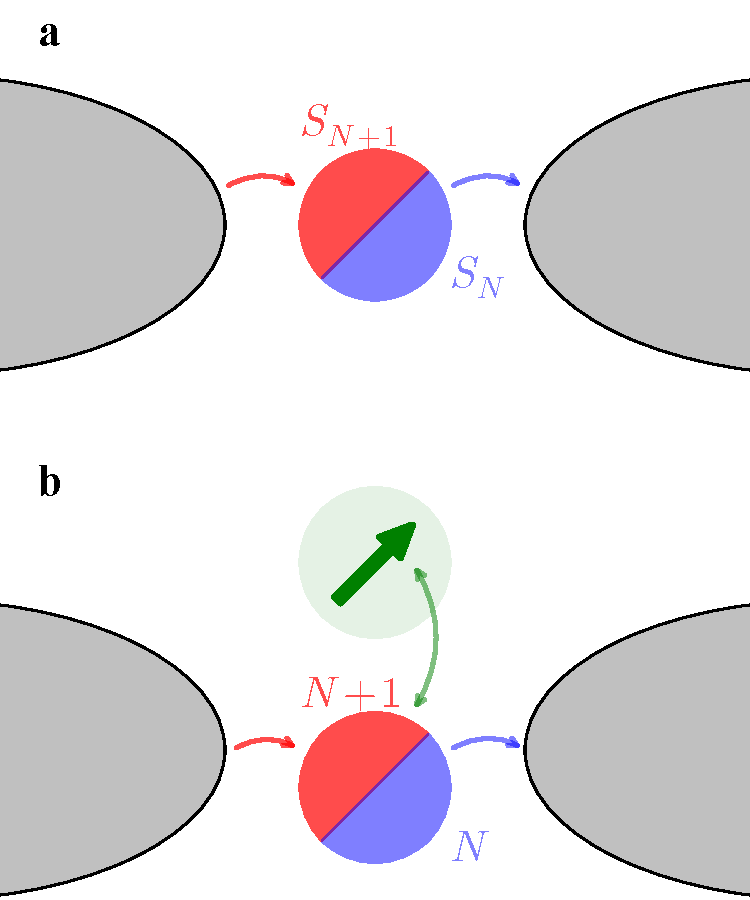
\includegraphics[scale=0.45]{Resultats/DirVsInd/DirVsInd.pdf} 
}
\parbox{7.5cm}{
\caption{\textbf{a} : configuration directe. Le centre magnétique est directement impliqué dans le transport électronique. Il oscille entre les états de charges $N$ et $N+1$. Cette oscillation entraîne une alternance entre les états magnétiques $S_{N}$ et $S_{N+1}$. \textbf{b} : configuration indirecte. Le centre magnétique n'est pas directement couplé au transport électronique mais par l'intermédiaire d'un point quantique. Cette dernière oscille entre deux états de charge $N$ et $N+1$, ces derniers étant influencé par l'état magnétique du centre magnétique, du fait d'une interaction~(exchange, dipolaire etc.).}
\label{DirVsInd}
}
\end{figure}


\subsection{Le couplage magnétisme-transport}
Dans la configuration directe présentée précédemment, le couplage entre le courant et le magnétisme est aisé à comprendre, les électrons participant au premier étant également directement impliqués dans le second. En revanche, dans la configuration indirecte, le couplage entre ces deux domaines peut avoir plusieurs origines, mais la m\^eme conséquence : rendre l'énergie du point quantique, et donc son potentiel chimique, dépendante de l'état du centre magnétique. Cette dépendance est fonction de la nature de l'interaction, comme nous allons le montrer maintenant.

\subsubsection{Le couplage dipolaire}

\begin{figure}
\parbox{6.5cm}{
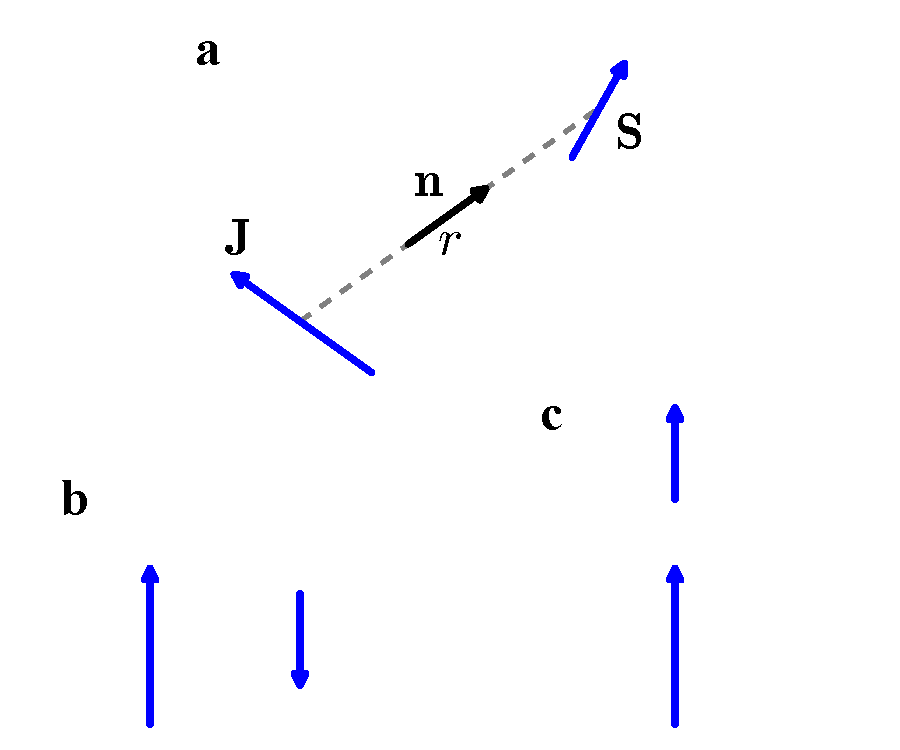
\includegraphics[scale=0.45]{Resultats/CDipolaire/CDipolaire.pdf} 
}
\parbox{7cm}{\caption{\textbf{a} : schéma représentatif du couplage dipolaire entre deux spins \textbf{J} et \textbf{S} séparés par une distance $r$. \textbf{b}(\textbf{c}) : configuration anti-ferromagnétique~(ferromagnétique) induite par le couplage dipolaire. Dans le cas du TbPc$_2$, l'axe facile étant perpendiculaire au plan des ligands, la configuration \textbf{c} est la configuration la plus vraisemblable.}
\label{dipolaire}
}
\end{figure}


Le couplage dipolaire est une interaction à distance entre deux moments magnétiques. Chacun de ces moments génère un champ dipolaire qui va venir agir sur le second, et vice versa. La modification en énergie induite est fonction de la distance séparant les deux dipôles, ainsi que de leur orientation relative. Ceci s'exprime par:
\begin{eqnarray}
E = -\frac{\mu_0^2 \mu_B^2}{4\pi r^3}(3\mathbf{SnJn} - \mathbf{SJ}) \nonumber
\end{eqnarray}
où $\mathbf{S}$ et $\mathbf{J}$ sont les spins associés aux deux moments magnétiques, $r$ la distance qui les sépare et $\mathbf{n}$ le vecteur unitaire reliant les deux moments (cf Fig.\ref{dipolaire}.a). En terme d'opérateur, cette expression peut se réécrire :
\begin{eqnarray}
E = -\frac{\mu_0^2 \mu_B^2}{4\pi r^3}(1 - 3 \cos^2 \theta) \lbrace S_zJ_z - \frac{1}{4}(J_+S_- + J_-S_+)\rbrace \nonumber
\end{eqnarray}
où $\theta$ est l'angle entre $\mathbf{S}$ et $\mathbf{J}$.

Plusieurs remarques s'imposent. Premièrement, l'intensité de l'interaction est proportionnelle à l'inverse de la distance au cube. Elle devient très rapidement négligeable : pour un spin $J=6$, elle ne vaut plus que $10$\,mT à $1$\,nm. Deuxièmement, en fonction de l'angle $\theta$, on peut imaginer deux configurations opposées : dans la situation de la Fig.\ref{dipolaire}.b, le couplage abouti à une organisation anti-ferromagnétique; dans celle présentée dans la Fig.\ref{dipolaire}.c, le couplage est au contraire ferromagnétique.

Comme nous l'avons vu précédemment, dans le cas du TbPc$_{2}$, la seule transition possible à basse température est $J_z=\pm6 \rightarrow J_z \mp 6$. En conséquence, la variation du potentiel chimique du point quantique sonde $\mu_{QD}$ est liée au renversement du moment magnétique par :
\begin{eqnarray}
\Delta \mu_{QD} = -\frac{\mu_0^2 \mu_B^2}{2\pi r^3}S_z\Delta J_z(1 - 3 \cos^2 \theta)   \nonumber
\end{eqnarray}
Celle-ci est directement proportionnelle à $\Delta J_z$.


\subsubsection{Le couplage d'échange}
Le couplage d'échange est une interaction de contact entre deux moments magnétiques. Il résulte d'un recouvrement des fonctions d'onde et peut favoriser deux situations opposées : si l'interaction est de type ferromagnétique, les spins s'alignent entre eux ; si elle est de type anti-ferromagnétique, l'orientation entre spin est opposée. Cette interaction s'exprime comme suit :
\begin{eqnarray}
E = A\mathbf{SJ} \nonumber
\end{eqnarray}
où $A$ est la constante d'échange. Lorsque $A>0$, le couplage est anti-ferromagnétique, si $A<0$, il est ferromagnétique. La constante d'échange peut prendre des valeurs élevées en énergie : dans le cas du N@C$_{60}$ par exemple, la valeur de l'échange entre le spin de l'azote et les électrons du C$_{60}$ a été mesurée comme étant supérieure à 4\,T~\cite{Roch2011}. Si l'on tient compte des considérations évoquées dans le cas du couplage dipolaire, la modification d\^ue à l'interaction d'échange qu’entraîne un retournement de l'aimantation peut s'exprimer de la façon suivante :
\begin{eqnarray}
\Delta \mu_{QD} = AS_z\Delta J_z\nonumber
\end{eqnarray}
Cette expression est semblable à celle obtenue pour le couplage dipolaire. La principale différence réside dans l'intensité de l'interaction : si celle-ci est de l'ordre du $mT$, elle est certainement dipolaire; si elle est de quelques dizaines de $mT$, l'interaction d'échange est certainement l'interaction dominante.

\subsubsection{Le couplage magnéto-Coulomb}
L'origine de ce couplage est électrostatique. Il a été mis en évidence dans les vannes de spin~\cite{Molen2006}, puis étudié dans le cas de nanotubes couplés à des particules magnétiques~\cite{Datta2011}. Si l'on considère un point quantique et un centre magnétique, cette interaction va coupler le potentiel chimique du premier à celui du second de telle sorte que :
\begin{eqnarray}
\Delta \mu_{QD} = C_{mc} \Delta \mu_{CM}
\end{eqnarray}
où $C_{mc}$ est la constante de couplage et $\Delta \mu_{CM}$ la variation du potentiel chimique du centre magnétique. Cette expression peut être simplifiée, au regard des remarques précédentes, de la façon suivante :
\begin{eqnarray}
\Delta \mu_{QD} = C_{mc} g \mu_B  \Delta J_z B_z
\end{eqnarray}
Contrairement aux expressions précédentes, la variation du potentiel chimique associée à un retournement de l'aimantation n'est pas constante mais dépend du champ magnétique appliqué, ce qui rend cette dernière facile à identifier.

Après avoir cerné les mécanismes pouvant être en jeux dans notre système, nous allons maintenant nous consacrer à l'étude détaillée de ses propriétés. Pour cela, nous présenterons rapidement la signature en transport de ce dernier, puis nous analyserons en détail le, ou les mécanismes, responsables du couplage entre magnétisme et transport électronique.

\section{Description de notre échantillon}
Avant de procéder à l'étude du magnétisme moléculaire, il est important de comprendre comment ce dernier interagit avec les électrons impliqués dans le transport. Il nous faut, pour cela, identifier la configuration de notre échantillon : directe ou indirecte. Ensuite, il est nécessaire de caractériser la ou les interactions assurant le couplage entre magnétisme et transport électronique.


\subsection{Signature en transport}

Avant d'étudier en détail la réponse magnétique de notre système, il est important de savoir si l'on se trouve en configuration directe ou indirecte. La première est généralement rencontrée lorsque l'on piège une molécule au sein d'un interstice nanométrique, constitué par les électrodes de source et de drain.

Dans le cas du TbPc$_{2}$, cette hypothèse est cependant peut vraisemblable. En effet, une configuration directe signifie que l'on modifie le nombre d'électrons impliqués dans le magnétisme. Dans notre cas, cela reviendrait à changer le nombre d'électron de la couche $4f$ de l'atome de terbium, et requerrait une énergie de l'ordre de l'électron-Volt. Cependant, on peut s'attendre à trouver une situation hybride dans laquelle l'état de charge de la molécule est modifié, mais cette modification n'affecte que les ligands, et laisse les propriétés du centre magnétique intacte. On peut qualifier cette configuration d'indirecte dans la mesure ou le point quantique n'est constitué que des ligands, le centre magnétique n'étant pas impliqué dans le transport électronique.

\begin{figure}
\parbox{7cm}{
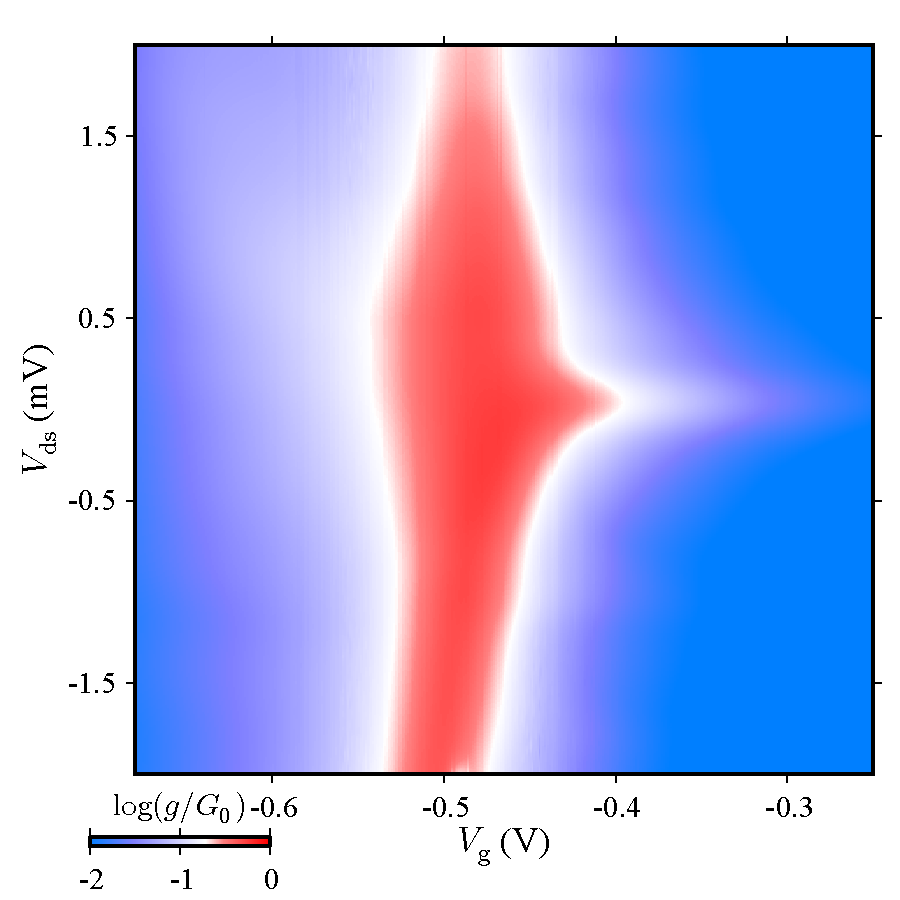
\includegraphics[scale=0.45]{Resultats/CoulombMap/CoulombMap.pdf} 
}
\parbox{6.5cm}{\caption{Diagramme de Coulomb montrant la mesure en conductance différentielle de notre échantillon, en fonction de la tension de grille $V_{\rm{g}}$ et la tension source drain $V_{\rm{ds}}$.}
\label{coulomb_map}
}
\end{figure}

Afin de confirmer cette hypothèse, nous avons mesuré la conductance différentielle de notre échantillon en fonction des tensions source-drain et de grille. La Fig.\ref{coulomb_map} présente le diagramme de stabilité obtenu dans lequel un pic de conductance est observable pour $V_{\rm{g}}=-0.5\,V$. Celui-ci correspond à un changement d'état de charge de notre point quantique, ce dernier étant de $N$ à gauche et de $N+1$ à droite. Le diamant de Coulomb habituellement rencontré dans ce type de mesure n'est pas visible ici, certainement du fait d'un fort couplage au électrode, ainsi que d'un couplage tunnel asymétrique entre la source et le drain.

Un élément important de cette mesure est la présence d'une résonance à tension source-drain nulle, du côté droit du point de dégénérescence. Cette signature traduit la présence d'un moment magnétique sur notre point quantique, ce dernier venant interagir avec les électrons de la source et du drain : c'est l'effet Kondo~\cite{Kondo1964,Wilson1975,Goldhaber-Gordon1998}.
 Il a été initialement observé dans les matériaux massifs contenant des impuretés magnétiques, ces dernières venant se coupler aux électrons de conduction. Dans notre cas, l'impureté magnétique n'est rien d'autre que le moment magnétique de notre point quantique, les électrons de conduction provenant de la source et du drain. Ce couplage étant anti-ferromagnétique, l'effet Kondo a pour conséquence de venir ``écranter'' le moment magnétique, formant un singlet entre le spin 1/2 et les électrons de conduction.

Lorsque l'on traite ce phénomène dans le cas de boîtes quantiques, on peut en rendre compte par une densité d'état élevé au niveau de Fermi de la source et du drain. Elle donne lieu à la résonance en conductance différentielle, à tension source-drain nulle~\cite{Goldhaber-Gordon1998}, que nous observons dans nos mesures.

Lorsque l'on étudie l'effet Kondo en fonction du champ magnétique, on observe l'apparition de deux résonances, une à tension positive et l'autre à tension négative, comme le montre la Fig.\ref{analyse_interaction}.\textbf{d}. En analysant l'évolution de ces dernières, et notamment la pente à champ magnétique élevé, il est possible d'en déduire la nature du moment magnétique. Dans notre mesure, on retrouve l'écart Zeeman correspondant à un spin $1/2$, ce dernier étant simplement décalé comme nous le verrons dans la suite.

La présence de ce spin $1/2$ signifie tout d'abord que le transport n'implique pas directement notre centre magnétique dont le moment magnétique est de $J=6$. Il correspond à un point quantique dont le niveau électronique est à moitié rempli, laissant le spin de l'électron non apparié interagir avec les électrons de la source et du drain. Les états de charge du système sont donc pair à gauche du point de dégénérescence et impair à droite. De plus, comme nous allons le voir dans la suite, notre système est sensible au magnétisme de l'atome de terbium. \textbf{Nous sommes donc dans une configuration indirecte}. Dans ce cadre, on peut envisager trois interactions responsables du couplage entre notre centre magnétique et notre point quantique sonde : magnéto-Coulomb, couplage d'échange, et couplage dipolaire.

Nous allons maintenant identifier quelles sont la ou les interactions réellement en jeu.

\subsection{Amplitude des sauts de conductance}
Précédemment, nous avons montré que le courant traversant le système, et donc, la conductance différentielle mesurée $g$, était directement relié au potentiel chimique du point quantique. On peut résumer cette tendance par la relation suivante:
\begin{eqnarray}
\text{d}g = \frac{\partial g}{\partial \mu} \text{d} \mu
\end{eqnarray}
Lorsque $\frac{\partial g}{\partial \mu} = cst$, la variation observée en conductance est une mesure directe de la variation du potentiel chimique. De plus, en raison de l'effet Zeeman, le potentiel chimique varie linéairement avec le champ magnétique, de sorte que $\text{d}\mu \propto \text{d}B$. Pour avoir une lecture directe de la variation du potentiel chimique, il faut donc choisir un point de fonctionnement tel que $\frac{\partial g}{\partial B} = cst$. La Fig.\ref{analyse_interaction}.\textbf{a} montre une mesure de $g$ en fonction du champ magnétique $B$, et met en évidence les zones correspondantes. Dans ces zones, un saut en conductance est directement proportionnel à la variation du potentiel chimique. 

La mesure présentée à la Fig.\ref{analyse_interaction}.\textbf{b} montre clairement que la hauteur des sauts en conductance, et donc la variation du potentiel chimique, ne dépendent pas du champ magnétique. Or, \textbf{cette observation n'est pas compatible avec une interaction de type magnéto-Coulomb}, ce qui nous permet de l'exclure des mécanismes de coulage. On a donc à faire, soit à un couplage dipolaire, soit à un couplage d'échange. Seule l'analyse de l'intensité de l'interaction peut nous renseigner. C'est à sa détermination que nous allons nous attacher maintenant.

\begin{figure}
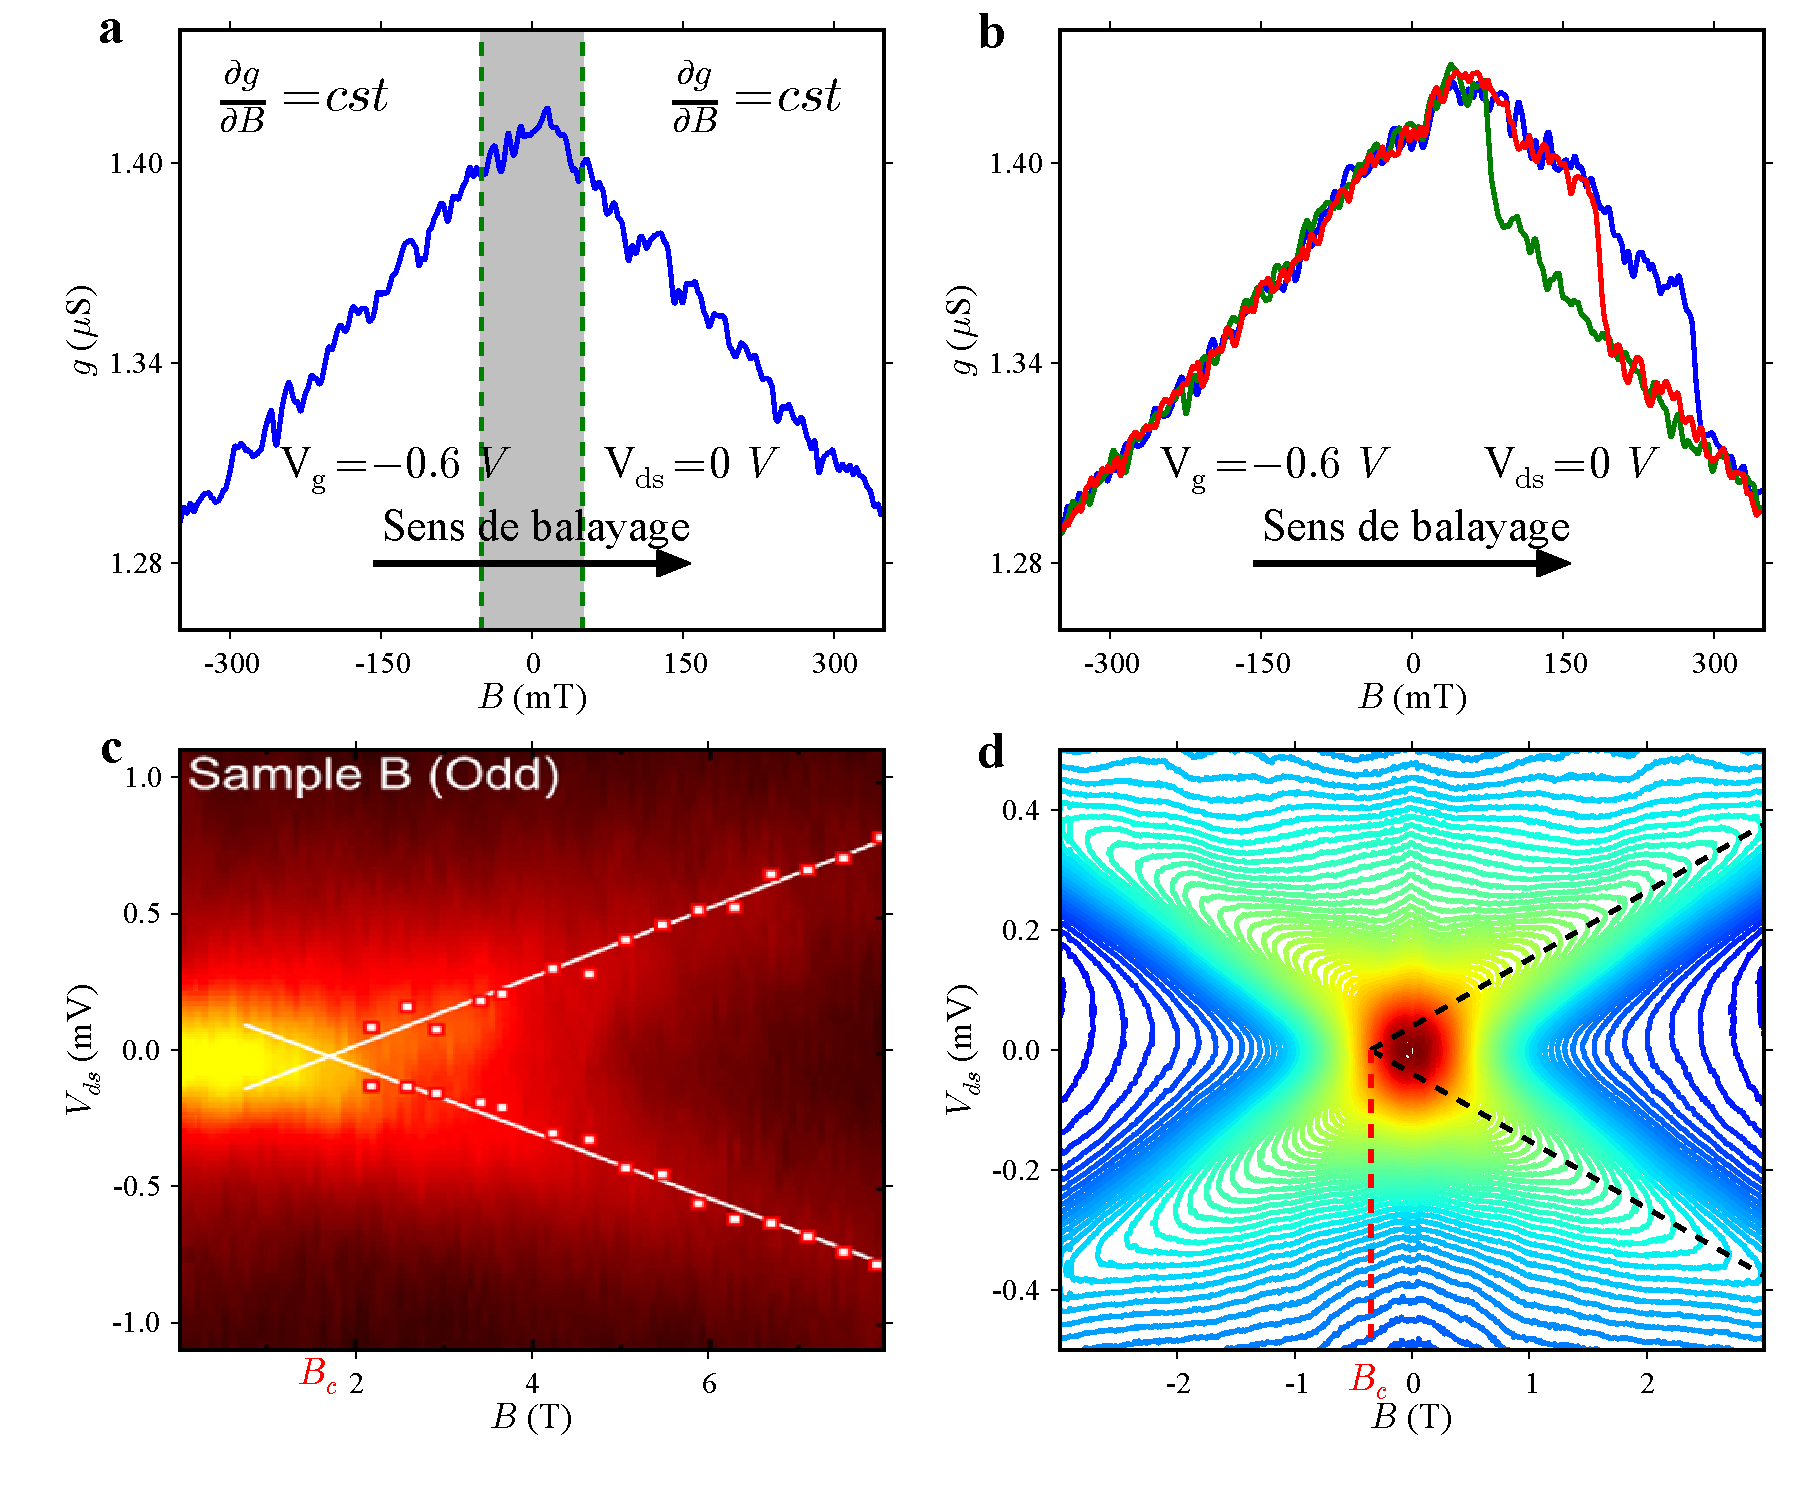
\includegraphics[scale=0.45]{Resultats/AmplJump/AmplJump.pdf} 
\caption{\textbf{a} - Mesure de la conductance différentielle en fonction du champ magnétique en l'absence de saut de conductance : les zones non grisées correspondent à des valeurs de champ magnétique où la variation de potentiel chimique $\Delta \mu$ est directement proportionnelle à la variation en conductance $\Delta g$. \textbf{b} - Mesure de trois sauts de conductance pour différentes valeurs de champ magnétique : celle-ci met en évidence l'indépendance de la variation $\Delta g$ vis-à-vis du champ magnétique appliqué. \textbf{c}(\textbf{d}) : Mesure en conductance différentielle de l'effet Kondo 1/2 en fonction du champ magnétique et de la tension source-drain pour un système sans~(soumis à l') interaction d'échange. L'extrapolation des maxima de conductance permet d'extraire la séparation Zeeman ainsi que la valeur du champ critique $B_c$.}
\label{analyse_interaction}
\end{figure}

\subsection{Intensité de l'interaction}
L'intensité d'une interaction peut être évaluée en comparant deux systèmes identiques : l'un soumis à ladite interaction; l'autre découplé de cette dernière. Pour réaliser cette expérience, on peut s'appuyer sur l'universalité d'un phénomène tel que l'effet Kondo. De part cette universalité, il nous est possible de comparer deux expériences différentes : l'une dans laquelle cet effet est mesuré sur un spin $1/2$ isolé, et une autre pour laquelle l'effet est mesuré dans la cas d'un spin $1/2$ couplé au moment magnétique de la molécule de TbPc$_2$. Nous allons pour cela comparer nos mesures à celles présentées dans~\cite{Roch2009}.

\subsubsection{L'effet Kondo $1/2$ non couplé}
La Fig.\ref{analyse_interaction}.c, tirée de \cite{Roch2009}, présente la mesure d'un effet Kondo 1/2 en fonction du champ magnétique et de la tension source drain. \`A champ magnétique et  à tension source-drain nuls, on observe un pic de conductance. Lorsque l'on applique un champ magnétique, ce pic s'étale, puis se divise en deux pics de conductance distincts. Cette séparation est directement induite par l'effet Zeeman. En extrapolant les maxima pour différentes valeurs du champ magnétique, on obtient une lecture de l'écartement Zeeman. En revanche, contrairement à ce que l'on pourrait attendre, les droites ne se croisent pas en $B=0$, mais en une valeur de champ fini $B_c$, supérieure à zéro. La valeur de $B_c$ est directement reliée à l'énergie Kondo $T_K$ par $0.5 k_bT_K = g \mu_B B_c$~\cite{Roch2009}. Autrement dit, il est nécessaire de fournir une énergie supérieure à celle de l'énergie Kondo pour "casser" le singlet formé par le nuage Kondo et l'électron du point quantique. Regardons maintenant ce qu'il en est de notre système couplé.

\subsubsection{Effet Kondo $1/2$ couplé} 
Si l'on effectue cette étude dans le cas de l'effet Kondo 1/2 couplé, on observe le même comportement général. Les pentes des droites extraites des extrema confirment qu'il s'agit d'un effet Kondo de spin 1/2. En revanche, la valeur de $B_c$ est maintenant négative. Tout se passe comme si le singlet était déjà "cassé" à champ magnétique nul. 

\textbf{Cette première observation nous permet d'éliminer l'interaction d'échange anti-ferromagnétique}. En effet, cette dernière aurait tendance, tout comme l'effet Kondo, à décaler $B_c$ vers des valeurs plus élevées de champ magnétique. On a donc à faire, soit à une interaction dipolaire, soit à une interaction d'échange ferromagnétique.

Une estimation basse de l'intensité de l'interaction, de l'ordre de plusieurs dizaines de milli-Tesla, est directement donnée par la valeur absolue de $B_c$. \textbf{Au regard des dimensions du système qui place le ligand à environ 1\,nm du centre magnétique, l'interaction dipolaire ne peut pas avoir une telle intensité}, comme nous l'avons vu précédemment. 

\textbf{Aux vues de ces différentes observations, nous pouvons conclure que l'interaction dominante est de type échange ferromagnétique}.

\section{Analyse des sauts en conductance}
L'analyse des sauts de conductance est à la base de notre méthode de détection. C'est de leur analyse statistique, que nous allons extraire les propriétés magnétiques de notre système. Le grand nombre de mesures~(jusqu'à 22000 par expérience) à traiter impose l'usage d'une méthode numérique. Celle-ci doit pouvoir extraire les paramètres essentiels des sauts de conductance : leurs positions en champ magnétique, leurs amplitudes et leurs signes. De plus, le point de fonctionnement, c'est-à-dire les tensions source-drain et grille appliquées, doivent être optimum afin de faciliter cette détection. 

Nous allons dans ce paragraphe décrire la méthode de détection des sauts. Ceci nous permettra, en particulier, de valider le lien entre variation de conductance et retournement de l'aimantation. Enfin, nous nous attarderons sur les critères de sélection du point de fonctionnement.

\begin{figure}
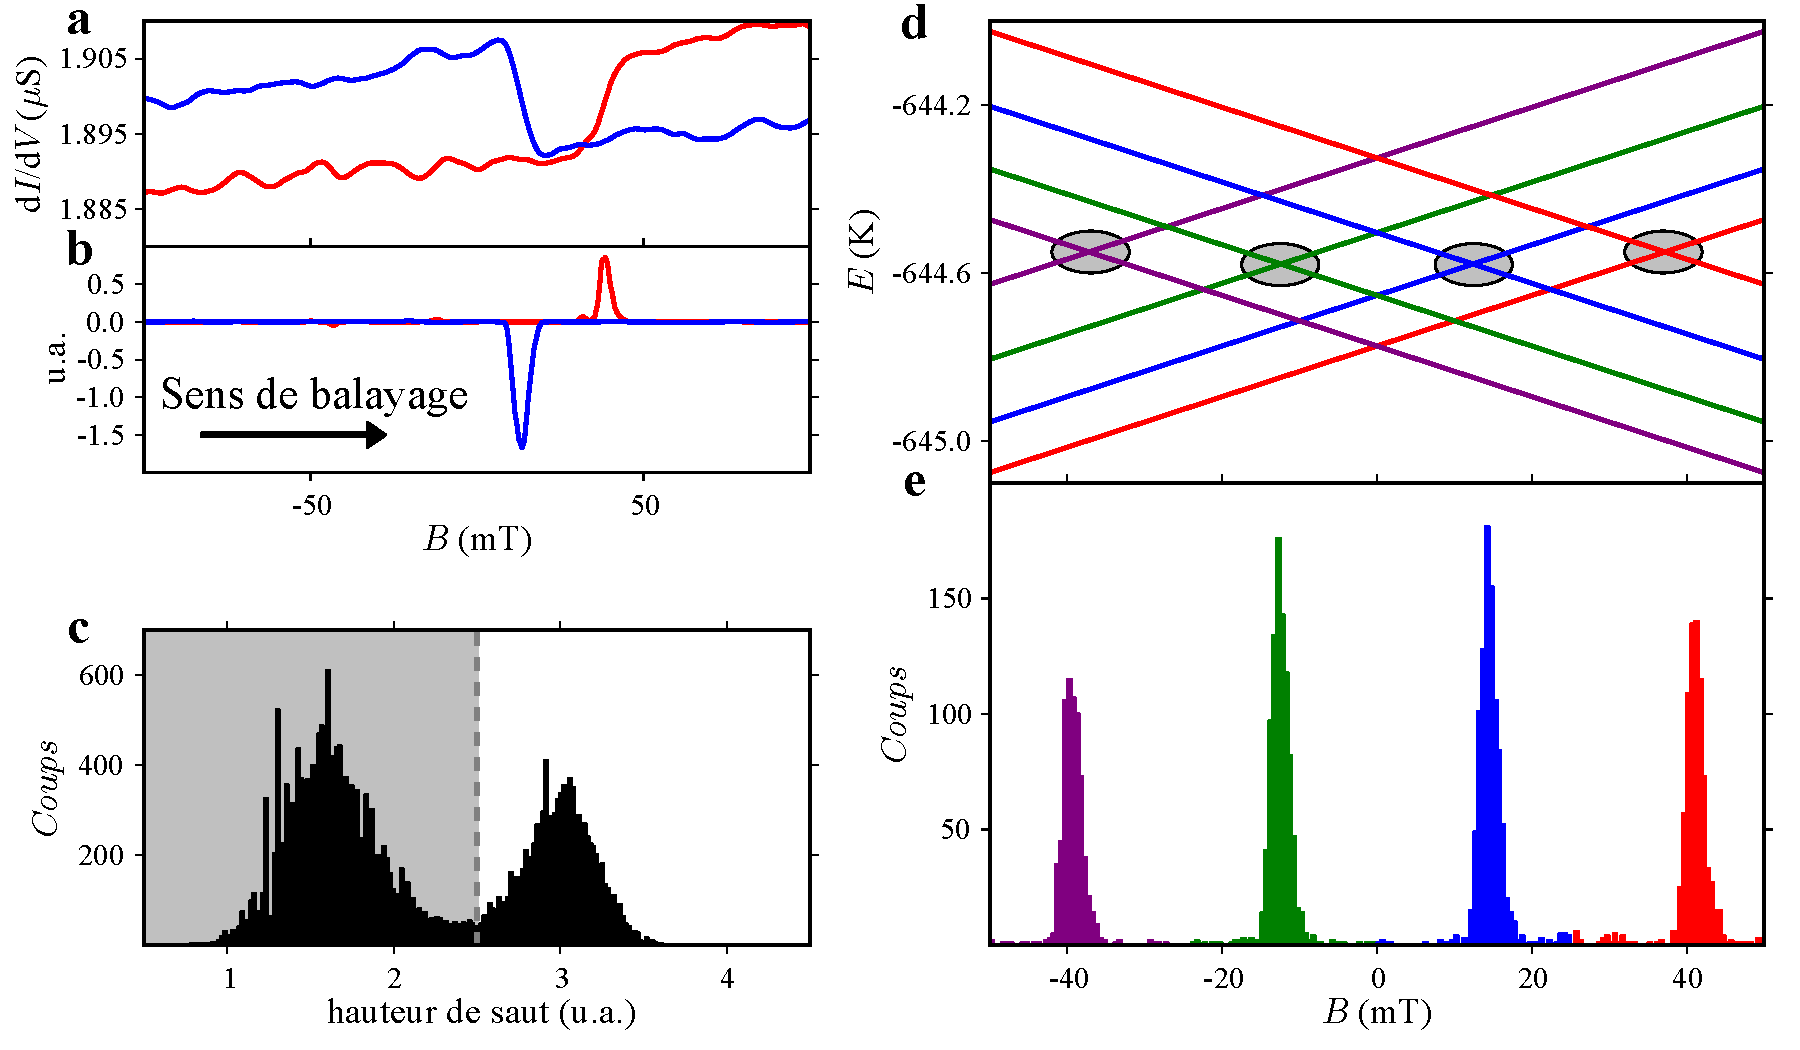
\includegraphics[scale=0.45]{Resultats/CondJump/CondJump.pdf} 
\caption{\textbf{a} - Mesure de deux sauts de conductance montrant deux variation $\Delta g$ de signes opposés. \textbf{b} - Signal correspondant à la mesure \textbf{a} filtrée : les sauts de conductance sont transformés en pics dont l'orientation (vers le haut ou vers le bas) dépend du signe de $\Delta g$. \textbf{c} - Statistique de la hauteur des sauts : cette dernière met en évidence deux distributions : celle contenue dans la zone grise correspond à de petites transitions relatives au bruit de mesure; la seconde distribution correspond au signal induit par le retournement de l'aimantation. \textbf{d} - Diagramme Zeeman de l'état fondamental de la molécule de TbPc$_2$ à faible champ : les anti-croisements donnant lieu au phénomène de QTM sont repérés par les cercles grisés. \textbf{e} - Statistique portant sur la position en champ des retournements de l'aimantation : quatre résonances sont clairement identifiables et correspondent aux quatre anti-croisements.}
\label{analyse_saut}
\end{figure}


\subsection{Méthode de détection}
La première étape de notre méthode de mesure est de détecter chaque saut en conductance, relatif à un retournement de l'aimantation. Une mesure type d'un saut de conductance est présentée dans la Fig.\ref{analyse_saut}.\textbf{a}. Il faut, dans un premier temps, rendre le signal plus facilement exploitable par l'application d'un filtre détaillé dans~\cite{Y.1995}. La Fig.\ref{analyse_saut}.\textbf{b} correspond au signal de la Fig.\ref{analyse_saut}.\textbf{a} après son application. Les sauts de conductances ont été convertis en pics, qu'il est facile d'extraire par une méthode des extrema. Le signe du saut de conductance est donné par l'orientation des pics : un changement positif correspond à un maximum; un changement négatif à un minimum.

Il faut ensuite procéder à l'analyse statistique de ces sauts. Pour cela, il est important de garder à l'esprit qu'il peut y avoir des mesures sans saut, le retournement de l'aimantation étant un événement probabiliste. Dans ce cas, les extrema détectés ne correspondront pas à un signal véritable mais à un artefact. Pour ne prendre en compte que le signal, on effectue une statistique de la hauteur des pics du signal filtré. La Fig.\ref{analyse_saut}.\textbf{c} présente le résultat d'une telle statistique pour 12000 mesures. Deux distributions sont clairement identifiables : une distribution avec de faibles sauts correspondant au bruit de mesure~(zone grisée); une distribution de sauts marqués correspondant à des retournements de l'aimantation. Cette statistique permet de fixer un seuil~(limite entre zone grisée et non grisée), et de filtrer les sauts détectés en conséquence.

A partir des sauts sélectionnés, on effectue une étude statistique des champs de retournement de l'aimantation. La Fig.\ref{analyse_saut}.\textbf{e} présente une telle statistique, effectuée sur 6000 mesures réalisées à faible champ. On peut facilement identifier quatre résonances, c'est-à-dire, quatre valeurs du champ pour lesquelles l'aimantation de la molécule a une forte probabilité de se retourner. 

En comparant cette mesure avec le diagramme Zeeman de la molécule de TbPc$_2$~(cf Fig.\ref{analyse_saut}.\textbf{d}), on peut associer chaque résonance à un des anti-croisements repérés par des cercles. Sachant que chacun d'eux correspond à une situation où le QTM est possible, on peut en déduire que la présence de ces résonances est la \textbf{mesure directe} du phénomène de QTM à l'échelle d'une seule molécule. 

De plus, chaque anti-croisement est associé à un unique état de spin nucléaire. La mesure de la position en champ magnétique du retournement de l'aimantation est donc une \textbf{mesure indirecte} de l'état de spin du noyau de terbium. C'est cette dernière propriété que nous utiliserons dans la suite pour étudier la dynamique du spin nucléaire.

\subsection{Interprétation physique de $\Delta g$}
Jusqu'à présent, nous n'avons pas utilisé le signe de $\Delta g$ comme élément d'analyse. Pourtant, dans le cadre de notre modèle, celui-ci donne accès à la nature de la transition : $J_z = \pm6 \rightarrow J_z = \mp 6$. Il existe une méthode expérimentale, basée sur la population thermique des spins nucléaires, permettant de vérifier notre hypothèse.

Supposons que l'on se place dans l'état initial $J_z=+6$ et $B<0$. Au regard du diagramme Zeeman de la Fig.\ref{TbPc2Zeeman}.\textbf{d}, et du fait de la relaxation, l'état de spin $I_z = -3/2$ devrait être le plus probablement mesuré. L'inverse est vrai pour l'état initial $J_z=-6$ et $B<0$. La Fig.\ref{analyse_signe_saut} présente une étude statistique des champs de retournement en fonction du signe de $\Delta g$. Lorsque $\Delta g> 0$~($\Delta g< 0$), l'état de spin nucléaire le plus probable est l'état $I_z = -3/2$~($I_z = +3/2$), ce qui correspond à un état initial $J_z=+6$~($J_z=-6$). $\Delta g> 0$~($\Delta g< 0$) correspond donc à la transition $J_z = +6 \rightarrow J_z =  - 6$~($J_z = -6 \rightarrow J_z =  + 6$).

\begin{figure}
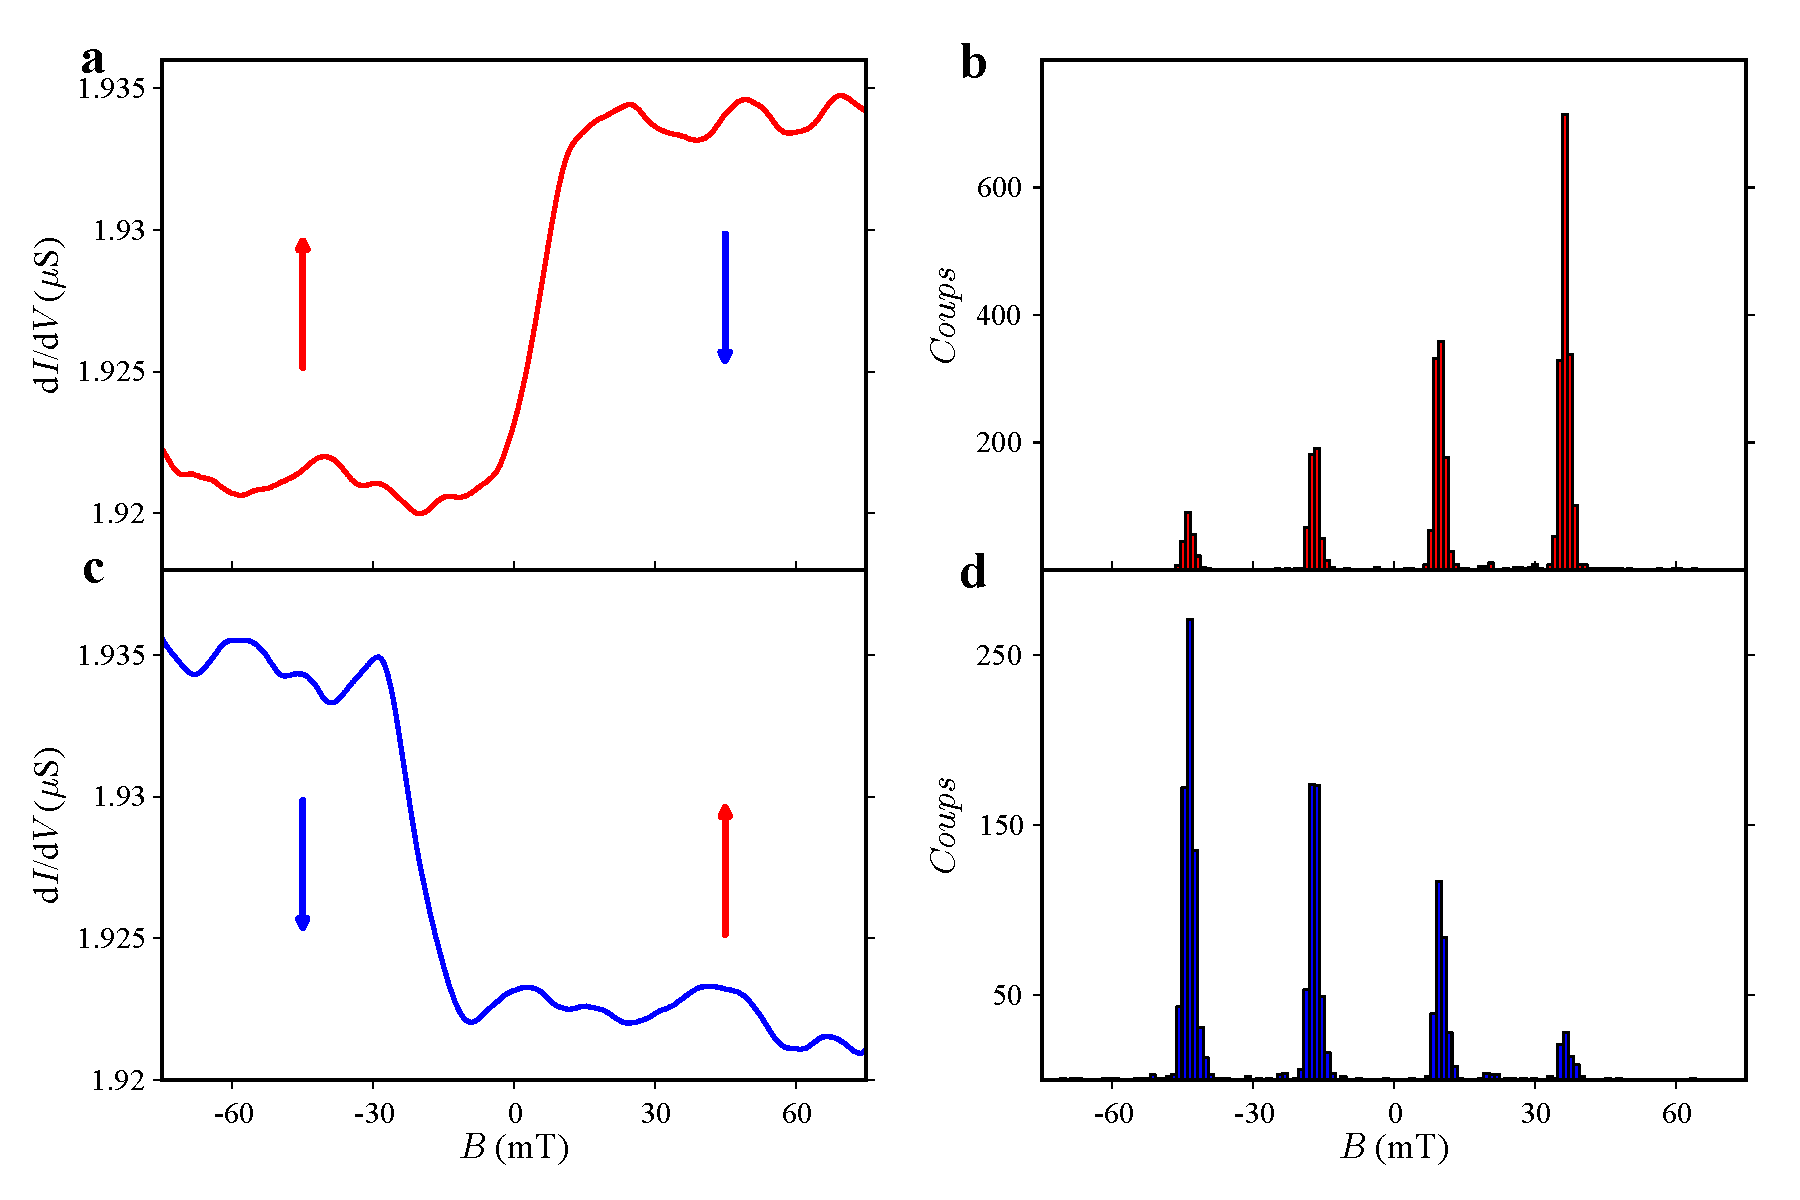
\includegraphics[scale=0.45]{Resultats/JumpSens/JumpSens.pdf} 
\caption{\textbf{a}(\textbf{c}) - Mesure d'un saut de conductance en fonction de l'état initial, la couleur de la courbe étant fonction de ce dernier. \textbf{c}(\textbf{d}) - Statistique des champs de retournement en fonction de l'état initial (signe de $\Delta g$) montrant clairement l'inversion de population des spins nucléaires. La couleur des histogrammes est donnée par l'état initial auxquels ils correspondent.}
\label{analyse_signe_saut}
\end{figure}

De cette étude, on peut donc affirmer de façon certaine, que la variation en conductance $\Delta g$ est directement liée au retournement de l'aimantation, et que son signe nous renseigne sur le sens de la transition.


\subsection{Choix du point de fonctionnement}
La zone où la variation de conductance est la plus sensible au potentiel chimique, se situe au niveau des points de dégénérescence. En effet, dans cette zone, la moindre variation du potentiel chimique entraîne une forte variation en courant. C'est donc dans cette zone, que l'on va logiquement se placer afin d'obtenir une sensibilité maximale. Dans un système idéal, on a $\left. \frac{\partial g}{\partial \mu}\right|_{\text{d}} = \left. -\frac{\partial g}{\partial \mu}\right|_{\text{g}}$, où $d$ et $g$ signifient à droite et à gauche du point de dégénérescence. Ceci a notamment été mis en évidence dans le cadre de nanoparticules magnétiques couplées par effet magnéto-Coulomb à un nanotube~\cite{Datta2011}.

\begin{figure}
\parbox{7cm}{
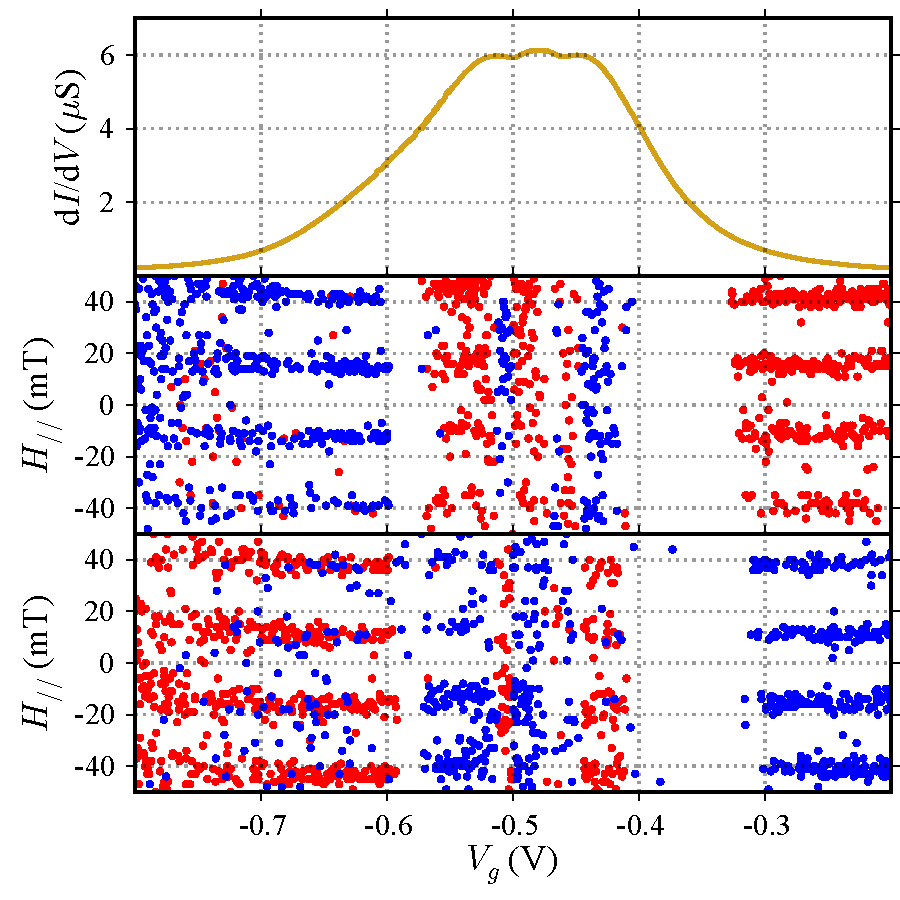
\includegraphics[scale=0.45]{Resultats/PointFonct/PointFonct.pdf} 
}
\parbox{6.5cm}{\caption{\textbf{Panel haut} - Mesure de la conductance différentielle en fonction de la tension de grille $V_g$ à tension source-drain nulle. \textbf{Panel du milieu~(bas)} - Mesure du signe de $\Delta g$ en fonction de la tension de grille $V_g$ et du champ transverse $H_{//}$ durant la trace~(retrace) : les points rouges correspondent à $\Delta g >0$; les points bleus à $\Delta g <0$. Les zones blanches dénotent des valeurs de tension de grille pour lesquelles le signal magnétique n'est pas résolu.}
\label{point_fonctio}
}
\end{figure}

Dans notre système, cette propriété n'est pas respectée et le résultat obtenu est plus complexe. La Fig.\ref{point_fonctio} montre le signe du changement de conductance correspondant à un retournement, en fonction de la tension de grille $V_g$. On observe trois types de zones : les zones où le signal est trop faible pour être détecté; des zones où le bruit généré par les phénomènes de transport masque le signal magnétique; enfin des zones où le signal magnétique est net et les résonances clairement visibles. Dans ces dernières, on observe des transitions d'un signe à l'autre similaire à un changement de signe de $\frac{\partial g}{\partial \mu}$. Notre système est en cela relativement éloigné du système idéal que nous avons utilisé jusqu'à maintenant. L'origine des zones de transitions ne nous apparaît toujours pas claire. En revanche, lorsque l'on s'éloigne des zones à forte conductance, le système se comporte de la manière attendue, avec un changement dans le signe $\frac{\partial g}{\partial \mu}$, de part et d'autre du point de dégénérescence.

Dans la suite, nous nous placerons loin des zones de transition, afin d'éviter toute mauvaise interprétation dans le signe de $\Delta g$.


\subsection{Procédure d'alignement}

L'une des caractéristiques principales d'un aimant moléculaire est de posséder un axe facile d'aimantation, c'est-à-dire, un axe le long duquel le moment magnétique "préfère" s'aligner. C'est suivant cet axe que le champ magnétique nécessaire au retournement de l'aimantation est le plus faible. Pour cette raison, il est indispensable de l'identifier de façon à minimiser le champ magnétique à appliquer à l'échantillon. Dans le cas d'un mauvais alignement, seule la projection du champ magnétique appliqué suivant l'axe facile contribue au retournement. Dans le cas extrême où le champ appliqué serait perpendiculaire à cet axe, aucun retournement ne pourrait être observé.

Expérimentalement, cette anisotropie magnétique peut être mise en évidence en mesurant l'hystérésis de l'aimantation. Hors, nous avons vu précédemment qu'un saut abrupt de conductance était observé en balayant le champ magnétique, et qu'il correspondait à un retournement de l'aimantation. Cela se traduit, lorsque l'on balaie le champ magnétique vers des valeurs positives, et inversement, par un hystérésis dans la mesure de la conductance, comme présenté dans la Fig.\ref{alignement}.\textbf{b}. Une lecture plus claire peut être obtenue en soustrayant l'aller au retour comme le montre la Fig.\ref{alignement}.\textbf{a}. En effectuant cette mesure pour différents angles de champ magnétique, on obtient la mesure présentée dans la Fig.\ref{alignement}.\textbf{c}. Celle-ci met en évidence un "axe facile" le long duquel le retournement se fait à faible champ, et un axe difficile le long duquel le champ n'est pas suffisant pour observer de retournement.

\begin{figure}
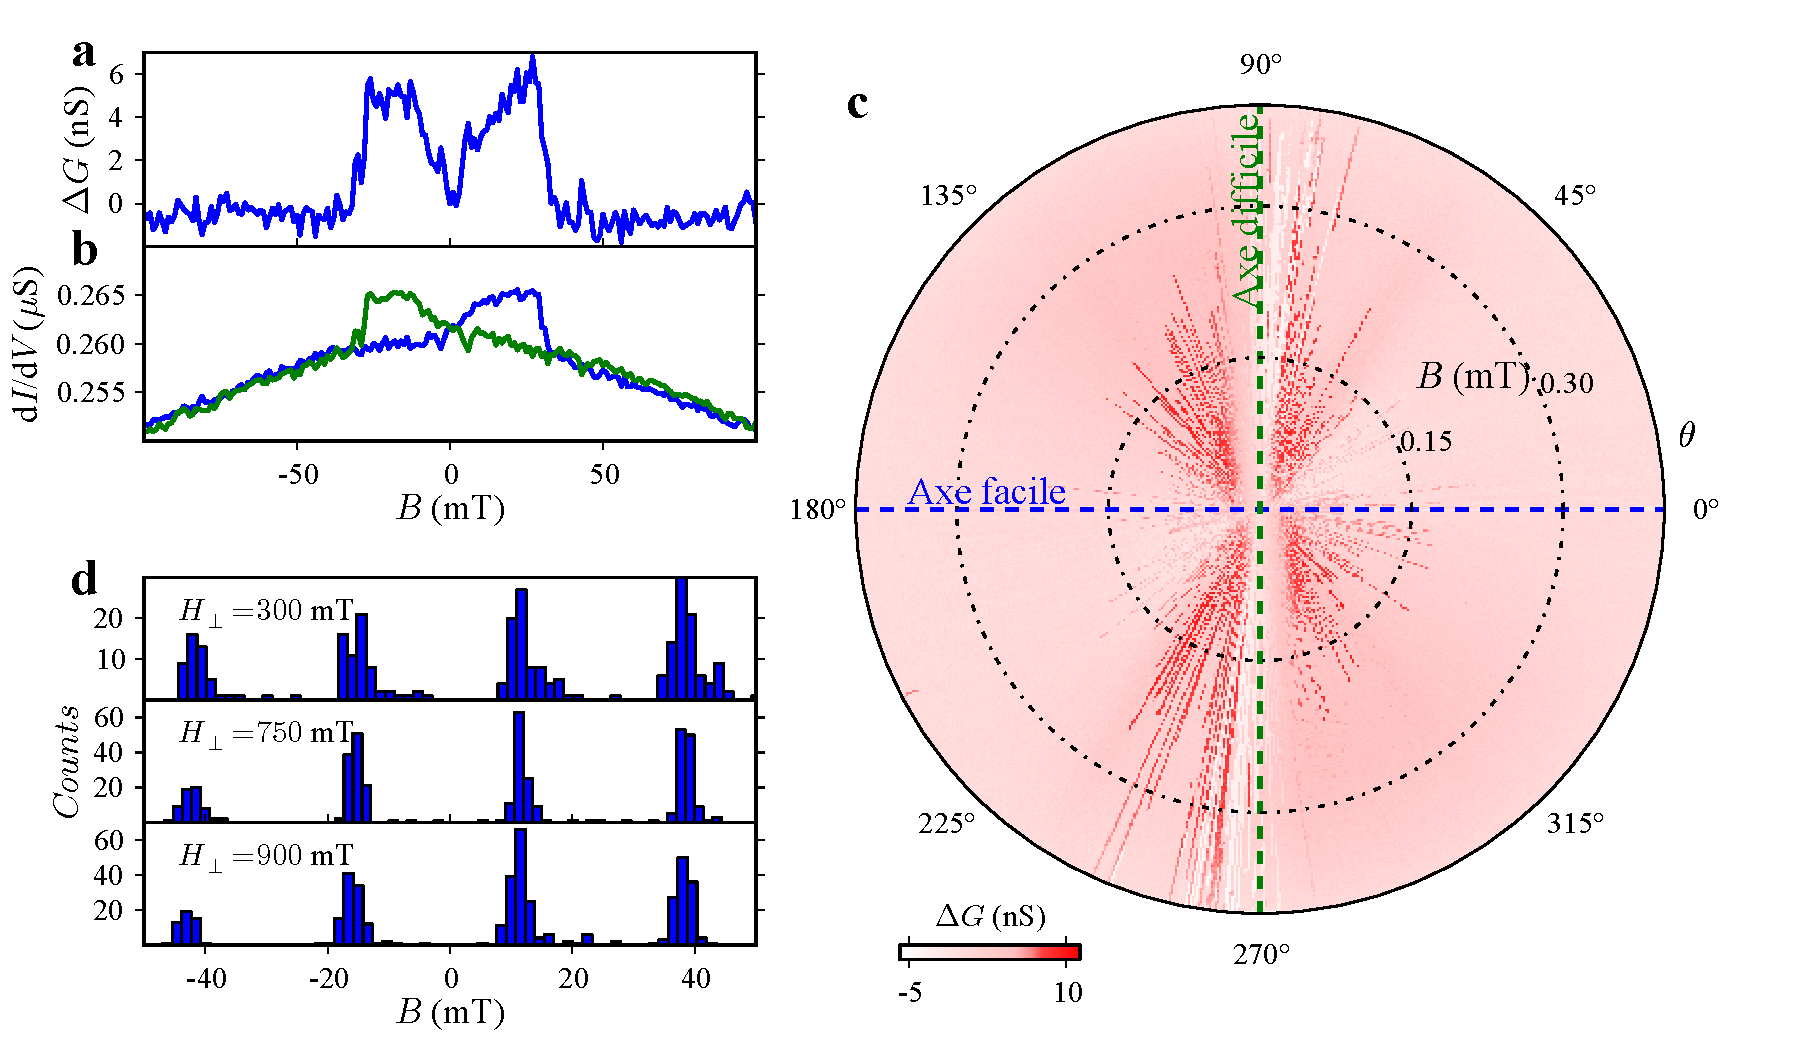
\includegraphics[scale=0.45]{Resultats/Alignement/Alignement.pdf} 
\caption{\textbf{a} : mesure de l’hystérésis en conductance en fonction du champ magnétique entre la trace et la retrace obtenu à partir de \textbf{b}. \textbf{b} : mesure de la conductance en fonction du champ magnétique pour la trace~(en vert) et la retrace~(en bleu). \textbf{c} : mesure de l'hystérésis en fonction de l'angle $\theta$. Les axes facile (retournement à faible champ) et difficile (retournement impossible) sont clairement identifiables. \textbf{d} : mesure de la position des résonances en champ magnétique parallèle en fonction du champ transverse. La position des résonances reste identique montrant le bon alignement de nos axes.}
\label{alignement}
\end{figure}

Cependant, il faut garder à l'esprit que ``l'axe facile" identifié par cette mesure, n'est en fait que la projection de celui-ci dans le plan défini par les deux axes magnétiques. Pour aligner notre dispositif expérimental avec l'axe facile de l'aimant moléculaire, il est préférable, dans un premier temps, d'identifier deux vecteurs du plan difficile. A cette fin, on effectue une deuxième mesure dans un plan différent, étape nécessaire à l'identification du plan difficile de l'aimant moléculaire. Sachant que l'axe facile est orthonormal à celui-ci, l'orientation de ce dernier est donnée par le produit vectoriel de deux vecteurs appartenant au plan difficile. Expérimentalement, l'angle $\theta$ permettant d'obtenir la mesure présentée dans la Fig.\ref{alignement}.\textbf{c} est défini à l'aide de deux bobines. L'angle $\phi$ nous permettant de faire la mesure dans deux plans différents est, quant à lui, obtenu par rotation de la dilution le long de l'axe d'une des bobines.


Afin de vérifier le bon alignement de nos axes magnétiques, nous avons mesuré la position des résonances à faible champ pour différent champs magnétiques appliqués suivant le plan difficile, que l'on appellera dans la suite champ transverse. Si l'alignement est correct, la projection d'un tel champ sur l'axe facile est nulle. La position des résonances ne devrait donc pas varier. La Fig.\ref{alignement}.d présente la position de ces résonances pour trois champs transverses, et confirme le bon alignement de nos axes magnétiques avec l'axe facile de la molécule.

\section{Magnétisme électronique}
Avant de nous intéresser au magnétisme nucléaire de notre système, nous allons nous attarder un instant sur le magnétisme électronique. Nous verrons tout d'abord comment il est possible de reconstituer le cycle d'hystérésis d'une molécule unique. On décrira notamment l'influence de l'environnement sur ce dernier, et nous montrerons comment, à l'aide d'un champ transverse, nous pouvons diminuer les interactions à faible champ. Nous verrons enfin que ce dernier peut également rendre l'extraction des données plus aisée.

\subsection{Reconstruction du cycle d’hystérésis}
Habituellement, afin d'accéder aux propriétés magnétiques des aimants moléculaires, on mesure ces derniers en assemblé, en considérant chacun d'eux comme étant isolé. L'aimantation ainsi mesurée représente les propriétés magnétiques moyennes d'un aimant moléculaire en fonction du champ magnétique.

Dans notre expérience, nous sommes parvenu pour la première fois à sonder les propriétés magnétiques d'un aimant moléculaire unique. Cette unicité nous oblige cependant à utiliser l'hypothèse ergodique à savoir : mesurer une assemblée de $N$ molécules identiques est équivalent à mesurer $N$ fois la même molécule. Pour le reste, la méthode de mesure est identique à celle employée avec la technique micro-SQUID. L'aimantation est amenée à saturation, ce qui revient, dans notre cas, à appliquer un champ magnétique suffisamment grand pour que l'aimantation de la molécule se retourne. Le champ magnétique est ensuite balayé continûment en effectuant des aller-retours, et la position en champ magnétique du retournement de l'aimantation est relevée. Ce cycle est effectué $N$ fois afin de pouvoir constituer une statistique~(dans nos expériences, $N$ a pris des valeurs comprises entre 1000 et 22000 selon les cas). A partir de cette statistique, nous pouvons reconstruire l'évolution de l'aimantation en fonction du champ magnétique. Pour cela on note $\mathscr{N}(B)$ le nombre de retournements mesurés avant le champ magnétique $B$ et on attribue le moment magnétique $\frac{M_s}{N}$ à chacun d'eux, $M_s$ étant l'aimantation à saturation et $N$ le nombre total de mesures. L'aimantation en fonction du champ magnétique prend alors la forme suivante :
\begin{eqnarray}
M(B) =\pm \frac{M_s}{N}(2\mathscr{N}(B) -1)\nonumber
\end{eqnarray}

Le signe est déterminé par celui du champ de saturation initial : positif pour un champ de saturation négatif; négatif pour un champ de saturation positif. Pour une comparaison plus aisée avec les mesures micro-SQUID, on peut ré-exprimer la formule précédente comme suit :
\begin{eqnarray}
\frac{M}{M_s}(B) =\pm \frac{1}{N} (2\mathscr{N}(B) -1)
\end{eqnarray}


Le résultat obtenu pour un champ de saturation de $\pm 400 \, mT$, une vitesse de balayage de $50\,mT.s^{-1}$, un champ transverse de $750\,mT$ et $N$ mesures, est présenté dans les Fig.\ref{CompAimant}\textbf{b}. Afin de faciliter l'analyse et les interprétations que je présenterai dans la suite, j'ai choisi de séparer les mesures en deux zones : à champ faible pour $|B|< 50\,mT$ et à champ fort pour $|B|>50\,mT$.

\begin{figure}
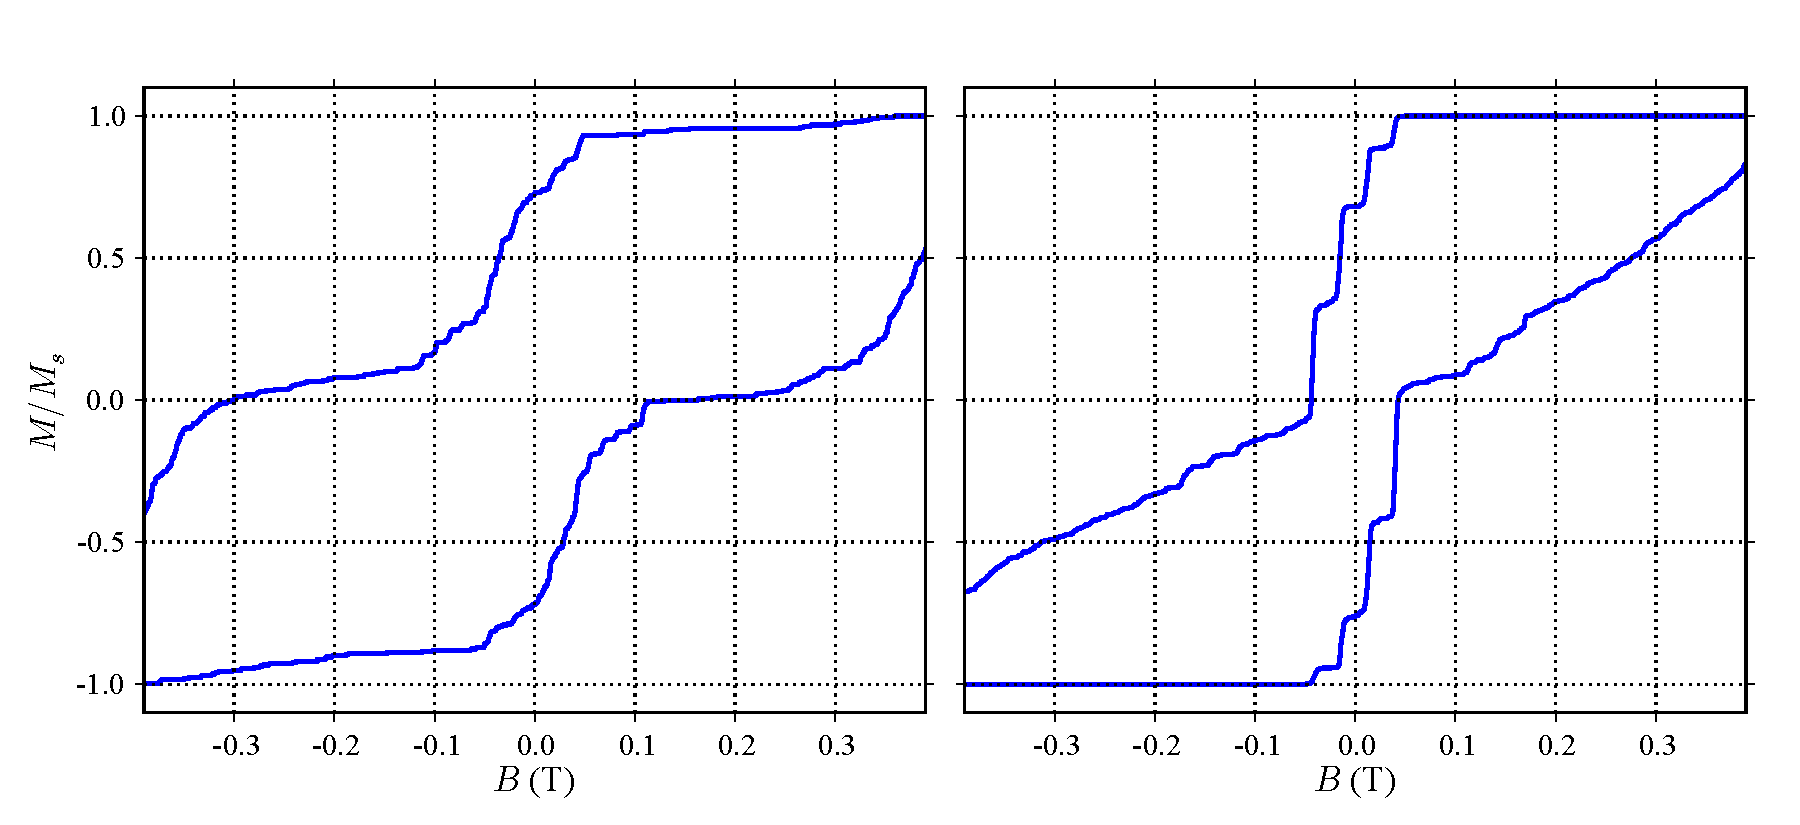
\includegraphics[scale=0.45]{Resultats/CompCrisMolUnique/CompCrisMolUnique.pdf} 
\caption{Hysteresis de la molécule TbPc$_2$ reconstruit à partir des mesures en transports sans champ transverse~(\textbf{a}), et avec un champ transverse de $750\,mT$~(\textbf{b}).}
\label{CompAimant}
\end{figure}

A faible champ, la structure en marche correspondante aux quatre anti-croisements de la Fig.\ref{TbPc2Zeeman}.\textbf{d}, caractéristique du phénomène de QTM~\cite{Thomas1996,Friedman1996}, est clairement visible. Il est à noter que, dans le cas de la mesure obtenue à partir d'un cristal moléculaire, un nombre plus élevé de marches est mesuré~(cf Fig.\ref{TbPc2Aimantation}). Ces dernières sont très certainement induites par des interactions entre les différents centres magnétiques du cristal~\cite{Wernsdorfer2002}, et ce, malgré la dilution à 10\%.

A champ fort là encore, il subsiste quelques différences entre la mesure micro-SQUID et celle obtenue avec notre système. Alors que, dans le cas d'un cristal moléculaire, le retournement assisté par le bain de phonons est le seul mécanisme impliqué, la présence  de marches superposées à un retournement continue est clairement visible dans le cas de notre système. Nous allons maintenant montrer que ces dernières sont très certainement induites par des interactions avec l'environnement.


\subsection{Le r\^ole du champ transverse}

La mesure de la Fig.\ref{CompAimant}.\textbf{b} a été réalisée pour un champ transverse de $750\,mT$. La présence de ce champ transverse n'est pas anodine, mais au contraire, nécessaire à l'obtention d'une mesure faiblement perturbée par l'environnement. En fait, la présence d'un champ transverse à deux conséquences : l'une physique, l'autre de l'ordre de la mise en œuvre de la détection. Nous allons maintenant détailler ces deux points.

\subsubsection{Conséquences physiques}
Notre aimant moléculaire, lorsqu'il est inséré dans l'interstice nanométrique, n'est pas, à proprement parlé, isolé. En effet, en plus de son environnement électrostatique inhérent à la configuration de type transistor à molécule unique, il peut également subir l'influence d'une autre molécule, d'une impureté magnétique piégée dans l'oxyde de grille, ou tout autre système susceptible d'échanger de l'énergie. Cependant, il est possible d'isoler notre aimant moléculaire de façon artificielle, par l'application d'un fort champ transverse. Ce dernier va aligner les systèmes magnétiques environnants, ne leur laissant plus la possibilité d'interagir avec l'aimant moléculaire. Les propriétés magnétiques de ce dernier sont, en revanche, peu perturbées par la présence de ce champ transverse.

L'amélioration dans la qualité de la mesure peut être apprécié, en comparant un cycle d'hystérésis reconstitué à partir d'une mesure sans champ transverse~(cf Fig.\ref{CompAimant}.\textbf{a}), et la même mesure réalisée avec un champ transverse de $750\,mT$~(cf Fig.\ref{CompAimant}.\textbf{b}). Dans le premier cas, une multitude de marches à faible champ est visible, et rend compte des couplages multiples entre l'aimant moléculaire et son environnement. Dans le second cas, à faible champ, on identifie clairement les marches relatives au QTM. A plus fort champ, on constate cependant la présence de marches secondaires, réminiscentes du couplage à l'environnement, initialement présent à faible champ.

Dans la suite, l'ensemble des mesures que je présenterai a été effectué avec un champ transverse de $750\,mT$.

\subsubsection{Impact sur la mise en œuvre}

La présence d'un champ transverse a également une conséquence sur la mise en oeuvre de la détection. Comme nous l'avons présenté dans la partie consacrée à la technique de détection, il est nécessaire, pour mesurer le retournement de l'aimantation de façon efficace, de se placer sur un point tel que $\frac{\partial g}{\partial B} = cst$. Or, à faible champ, cette relation n'est plus vérifiée et l'on observe un changement de signe de $\frac{\partial g}{\partial B}$  comme le montre la Fig.\ref{analyse_interaction}.\textbf{a}~(partie grisée), ce qui n'est pas sans poser de problèmes. D'autant plus que le phénomène de QTM se déroule également à champ faible.

Nous avons observé, pour notre échantillon, une légère anisotropie de la conductance en fonction du champ magnétique. Cela se traduit, lorsque l'on applique un champ transverse, par un décalage de la zone d'inversion du signe de $\frac{\partial g}{\partial B}$, comme le montre la mesure de la Fig.\ref{TransInfl}. On peut donc opérer des mesures, avec un signe de  $\frac{\partial g}{\partial B}$ constant sur la totalité de la plage de champ magnétique nécessaire à la caractérisation du phénomène de QTM.


\begin{figure}
\parbox{7cm}{
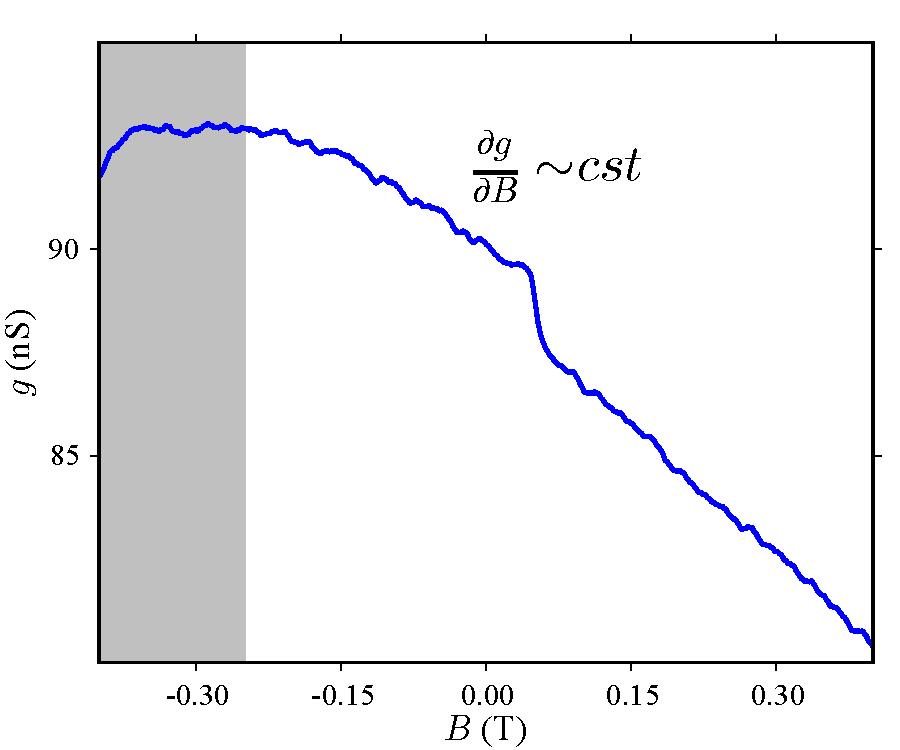
\includegraphics[scale=0.45]{Resultats/TransInfl/TransInfl.pdf} 
}
\parbox{6.5cm}{\caption{Mesure de la conductance différentielle $g$ pour un champ transverse $750\,mT$. La zone correspondant à $\frac{\partial g}{\partial B} \sim \rm{cst}$ s'étend sur toute la zone de mesure.}
\label{TransInfl}
}
\end{figure}




Cette propriété a le mérite de faciliter considérablement l'interprétation du signe de $\Delta g$, et améliore grandement la capacité de détection à faible champ magnétique. Il est désormais possible de se concentrer sur le magnétisme à faible champ et, en particulier, sur la dynamique du spin nucléaire. 

\section{Dynamique du spin nucléaire}
L’intérêt du spin nucléaire dans la cadre de l'information quantique, a été maintes fois mis en avant~\cite{Kane1998,Vandersypen2001,Leuenberger2003}. Mais avant de pouvoir manipuler les différents états de spin, il est nécessaire de connaître la dynamique de ce dernier, ainsi que l'influence que peut avoir notre technique de mesure sur ses états. En outre, compte tenu du courant qui circule dans le point quantique sonde, il est légitime de s'interroger quant à l'influence de l'environnement électrostatique, sur les processus de relaxation, mais aussi sur la température d'un spin nucléaire unique. 

\subsection{Temps de relaxation}

Le spin nucléaire, du fait de son couplage relativement faible à l’environnement, possède généralement un temps de vie élevé. Afin de pouvoir vérifier cette propriété, il nous faut pouvoir mesurer l'évolution des états du spin nucléaire en fonction du temps. 

\subsubsection{Procédure de mesure}
Nous avons choisi pour cela une technique simple consistant à mesurer l'état du spin nucléaire lors de deux mesures, en faisant varier le temps séparant ces dernières.

\begin{figure}
\centering 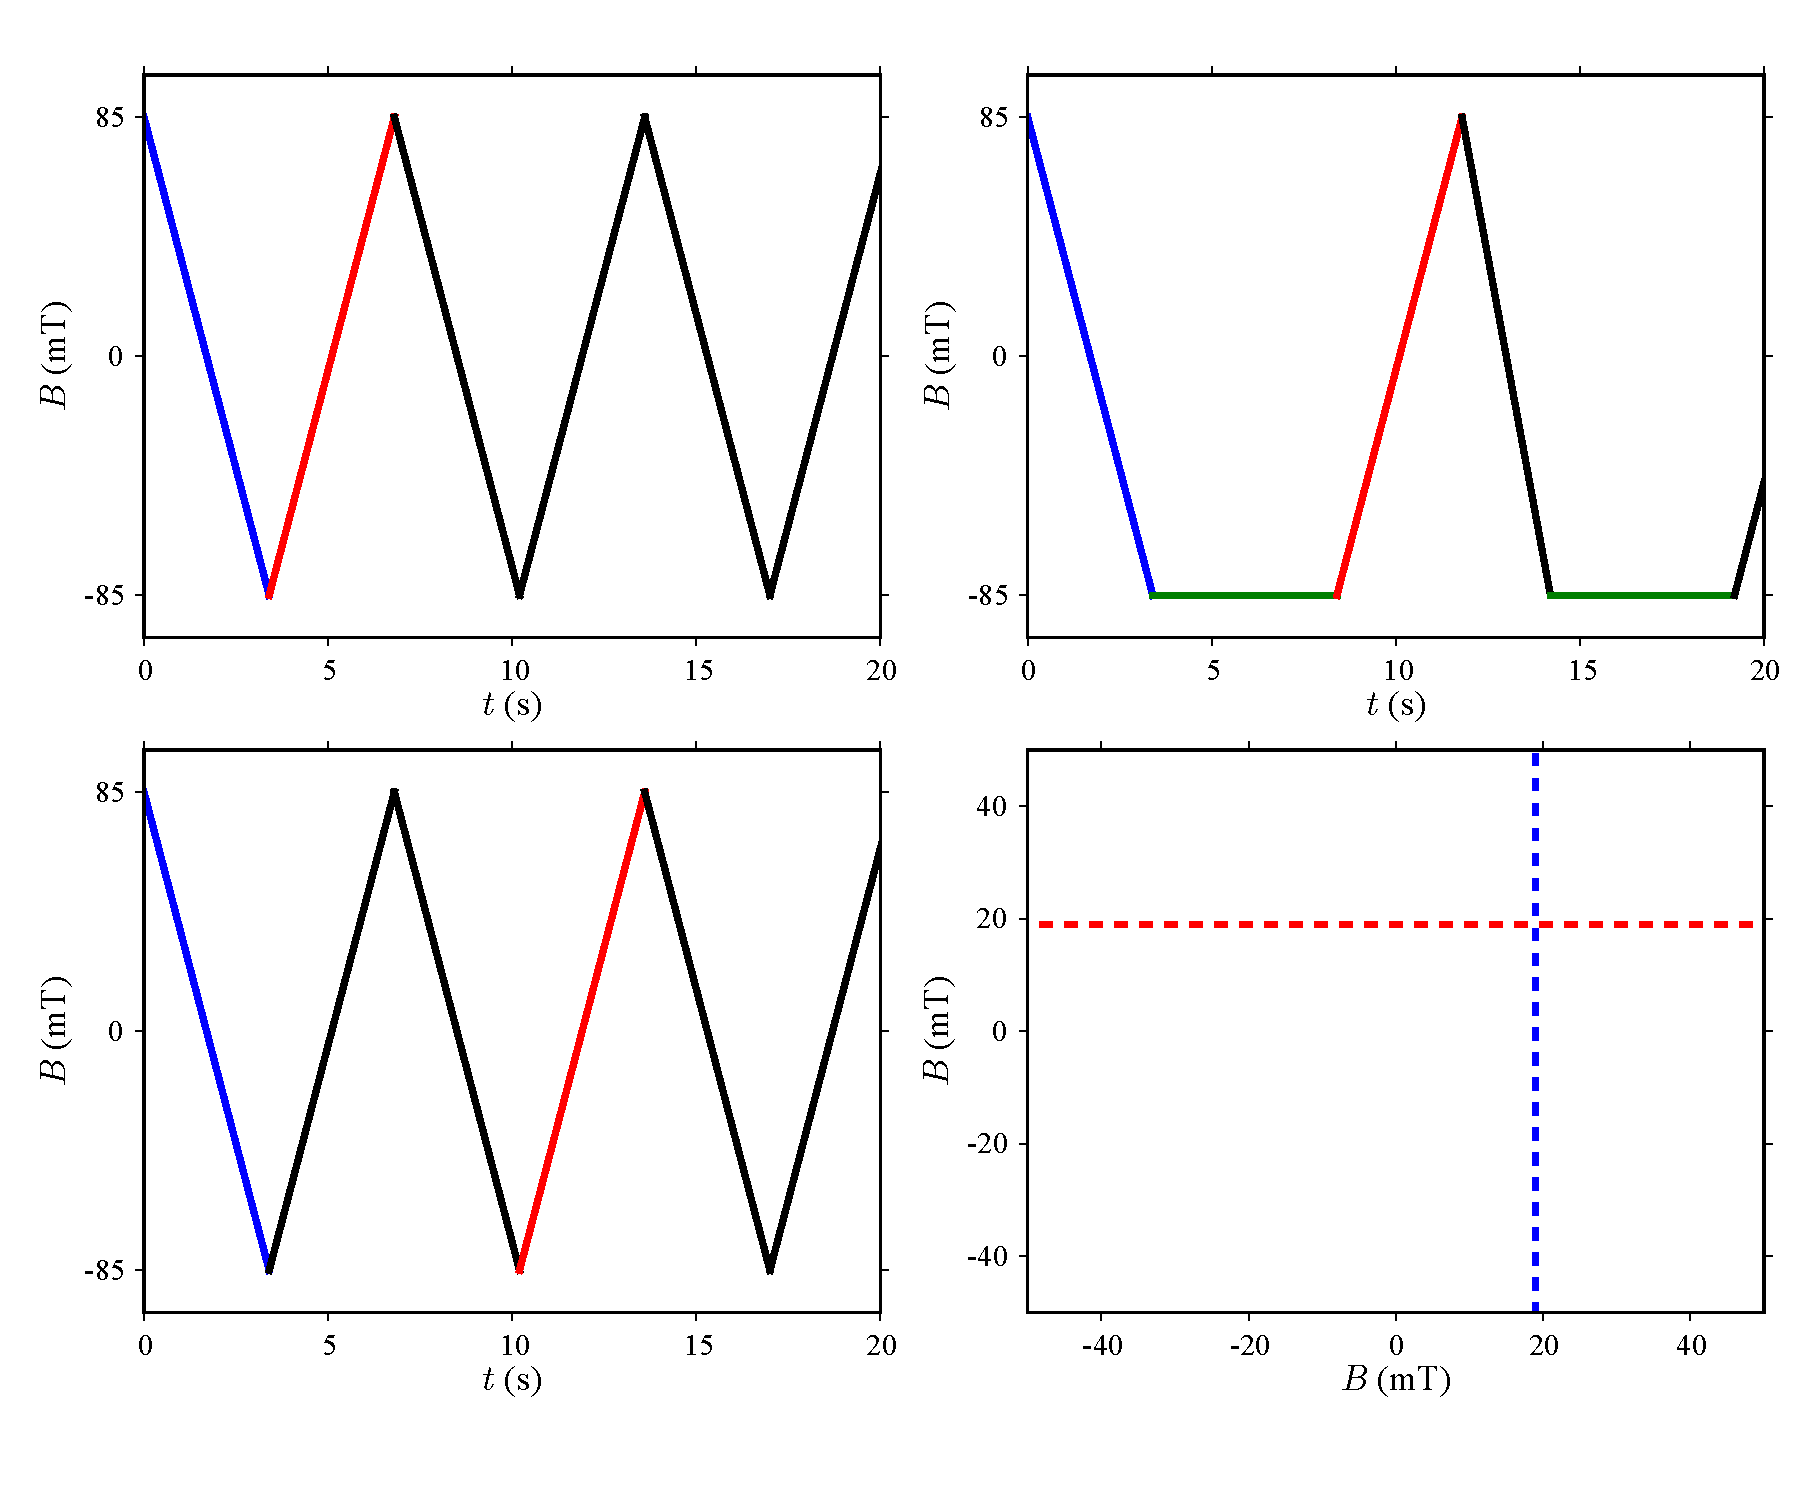
\includegraphics[scale=0.45]{Resultats/PostFig1/postfig1.pdf} 
\caption{\textbf{a}~(\textbf{b})~:~représentation de la procédure de mesure lorsqu'aucun temps d'attente~(un temps d'attente de 5\, secondes, représenté en vert) n'est inséré entre la retrace et la trace suivante. \textbf{c}~:~procédure de mesure correspondant à une corrélation du troisième ordre, deux mesures se situant entre les deux retournement considérés~(en bleu et en rouge). \textbf{d}~:~représentation d'une correlation dans un diagramme à deux dimensions.  La position en champ magnétique du retournement de l'aimantation obtenue durant les deux mesures est repérée sur les axes $x$, et $y$ par deux lignes dont le croisement va donner un point de corrélation. En répétant cette procédure un grand nombre de fois, un histogramme en deux dimensions de ces corrélations peut être obtenu~(cf Fig.\ref{correlations}).}
\label{procedure}
\end{figure}


Le point de polarisation est choisi afin d'être sensible au retournement de l'aimantation, tout en minimisant le courant traversant notre système; ce qui revient à choisir dans notre cas $V_g \sim -0.6\,V$ et $V_{ds}=0\,V$~(cf Fig.\ref{coulomb_map}). Le champ magnétique est, quant à lui, balayé à la vitesse de $50\,mT.s^{-1}$ entre $-85\,mT$ et $+85\,mT$, puisque nous nous intéressons à la physique du spin nucléaire, et donc, à la zone correspondant au anti-croisements.

Du fait de l'aspect chronophage de cette procédure~(jusqu'à plusieurs jours par mesure), nous avons choisi cinq temps d'attente différents~:~$0,\,5,\,10,\,20$ et $50$ secondes. Pour chacune de ces valeurs, $22000$\,balayages ont été effectués afin d'obtenir une statistique significative.
Les Fig.\ref{procedure}.\textbf{a} et \textbf{b} présente la processus de mesure sans temps d'attente~(Fig.\ref{procedure}.\textbf{a}) et avec un temps d'attente de 5\,secondes~(Fig.\ref{procedure}.\textbf{b}), la corrélation se faisant entre la retrace (en bleu) et la trace suivante (en rouge). Les données ainsi obtenues sont ensuite représentées dans un histogramme en deux dimensions (cf Fig.\ref{procedure}.\textbf{d}). La coordonnée suivant l'axe x est donnée par le position du retournement durant la trace, et la coordonnée suivant l'axe y est quant à elle donnée par la position du retournement durant la retrace.


\subsubsection{Résultats}

\begin{figure}
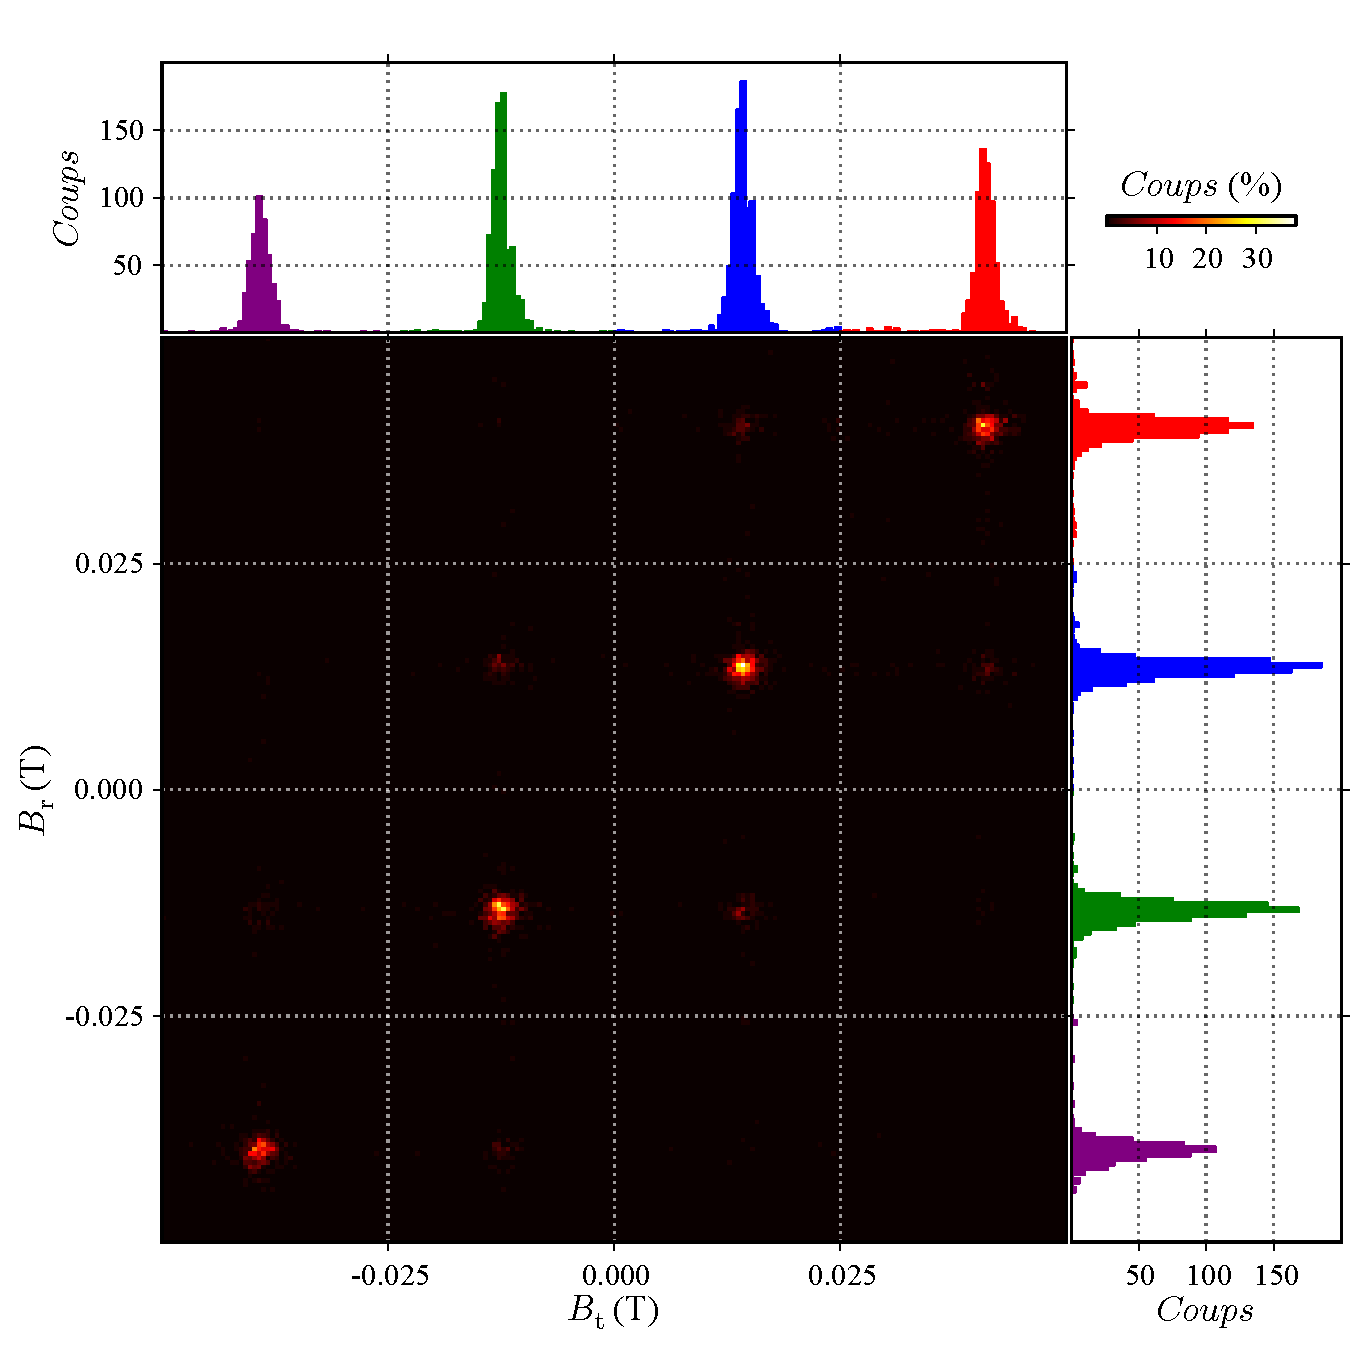
\includegraphics[scale=0.45]{Resultats/Hist2D/Hist2D.pdf} 
\caption{La cartographie couleur en deux dimensions représente l’histogramme de corrélation des champs de retournement ayant lieu durant la trace et la retrace. Celui-ci a été obtenu à partir de 22000 traces et retraces mesurées consécutivement, et sans temps d'attente. Les histogrammes à une dimension disposés le long des axes x et y représentent respectivement la statistique des positions en champ magnétique des retournements durant la trace et la retrace. La prépondérance des éléments diagonaux atteste de la préservation de l'état de spin entre deux mesures.}
\label{correlations}
\end{figure}


L'évolution des états du spin nucléaire est représenté à l'aide d'un histogramme à deux dimensions. Le champ de retournement de la première mesure est repéré en abscisse et celui mesuré lors de la seconde mesure est représenté en ordonnée. Dans une telle représentation, les éléments diagonaux rendent compte d'un état de spin nucléaire qui ne change pas entre les deux mesures. Les éléments hors-diagonaux représentent quant à eux, les cas où l'état de spin nucléaire varie de $\Delta m_z^I = \pm 1,2,3$, où $m_z^I$ est la projection du moment angulaire du spin nucléaire sur l'axe $z$. La Fig.\ref{correlations} présente une telle mesure pour un temps d'attente nul. Pour faciliter la lecture, les histogrammes des champs de retournement de la première et deuxième mesures ont été ajoutés.

La Fig.\ref{evolution_temps} montre l'évolution de cet histogramme en fonction du temps d'attente entre les deux mesures. Les éléments diagonaux dominent jusqu'à un temps d'attente de $20$ secondes, prouvant que le spin nucléaire demeure majoritairement inchangé sur ce laps de temps. En revanche, pour un temps d'attente de $50$ secondes, on constate que les éléments diagonaux ne sont plus prépondérants, signifiant le perte de l'état nucléaire entre les deux mesures. De plus, la résonance correspondant à l'état de spin $|-3/2 \rangle$ domine largement, ce qui traduit la tendance du système à évoluer vers l'équilibre thermodynamique, lorsque le temps d'attente devient trop élevé. Nous reviendrons sur ce dernier point dans la suite.

Il peut être intéressant de ce demander si une partie de la décohérence observée, n'est pas induite par notre technique de mesure.

\begin{figure}[h!]
\includegraphics[scale=0.45]{Resultats/HistTime/HistTime.pdf} 
\caption{La cartographie \textbf{a} (\textbf{b}, \textbf{c}, \textbf{d} et \textbf{e}) présente un histogramme 2D rendant compte de la corrélation entre deux mesures obtenues durant la trace et la retrace, ces dernières étant séparées d'un temps d'attente de 0 secondes (5, 10, 20 et 50 secondes). La prédominance des éléments diagonaux pour des temps d'attente allant au-delà de la dizaine de seconde, démontre le long temps de vie des états du spin nucléaire.}
\label{evolution_temps}
\end{figure}

\subsection{Perturbations induites par la mesure}
Il est également important d'évaluer l'influence de la mesure sur l'état de spin nucléaire, afin d'interprété de façon pertinente l'ensemble des mesures.

\subsubsection{Procédure de mesure}
Pour cela, nous avons choisi d'utiliser la méthode présentée précédemment, en observant non plus l'évolution de l'état nucléaire en fonction du temps, mais en fonction du nombre de mesures. Autrement dit, on effectue des corrélation d'ordre supérieur.

La Fig.\ref{procedure}.\textbf{c} présente la mesure d'une corrélation au troisième ordre, dans lequel la corrélation est faites entre la mesure obtenue durant un retrace~(bleu) et une trace~(rouge) séparées par deux balayages. Bien sûr, la corrélations peut s'effectuer indifféremment entre trace et/ou retrace. En effet, puisqu'il n'y a aucun temps d'attente entre les différents balayages, traces et retraces sont équivalentes.

Nous avons utilisé les données collectées sur 22000 balayages (11000 traces et autant de retraces) effectués sans temps d'attente, et les résultats ont également été présentés à l'aide d'un histogramme à deux dimensions, en utlisant la méthode introduite précédemment, la position du retournement durant la première mesure étant représentée sur l'axe x, et celui correspondant à la seconde mesure étant représenté sur l'axe y.

\subsubsection{Résultat}
La Fig.\ref{evolution_mesures} présente cette évolution après deux~(\textbf{a}), trois~(\textbf{b}), quatre~(\textbf{c}), cinq~(\textbf{d}) et six~(\textbf{e}) mesures. On constate qu'après 4 mesures, les éléments diagonaux dominent toujours, pour ne commencer à s'atténuer qu'au bout de 6 mesures. Il est important de noter que chaque mesure est, en moyenne, séparée de 4 secondes, et donc, dans le cas de 6 mesures, cela correspond à un temps total de plus de 20 secondes. Aux vues des résultats présentés dans la section précédente, on peut donc attribuer cette diminution de corrélation dans l'état du spin nucléaire aux processus de relaxation internes, la procédure de mesure elle-même n'affectant qu'à la marge le système. 

La méthode de mesure de l'état de spin nucléaire par l'intermédiaire du QTM se révèle donc peu invasive, ce qui permet d'étudier les propriétés du système, en négligeant son influence sur ce dernier. Elle peut aussi être utilisée afin d'extraire, sans trop de perturbation, la population des états de spin nucléaire.

\begin{figure}
\includegraphics[scale=0.45]{Resultats/MesureInfl/MesureInfl.pdf} 
\caption{La cartographie \textbf{a} (\textbf{b}, \textbf{c}, \textbf{d} et \textbf{e}) présente un histogramme en deux dimensions rendant compte de la corrélation entre les états de spin nucléaire après deux (trois, quatre, cinq et six) mesures. On constate qu'après six mesures, les éléments diagonaux sont toujours dominants, démontrant la faible influence de notre procédure de mesure sur l'état du spin nucléaire.}
\label{evolution_mesures}
\end{figure}

\subsection{Extraction des populations nucléaires}
Nous avons montré qu'on pouvait, à travers un histogramme des positions en champ des renversements, facilement identifier les différents états de spin. Nous allons utiliser cette m\^eme mesure en la présentant différemment. En effet, chaque retournement au voisinage d'une résonance peut \^etre attribué à un état de spin précis, les différentes résonances ne se recouvrant pas~(cf Fig.\ref{extract_pop}.\textbf{a}). En intégrant et en normalisant le nombre de mesures obtenues pour chaque état de spin nucléaire, on peut reconstruire leur distribution. 

Cependant, cette dernière contient en fait deux distributions, l'une relative à l'état initial $J_z=-6$ et l'autre $J_z=+6$. Il est cependant possible de les différencier à partir du signe du changement en conductance $\Delta g$, comme nous l'avons déjà montré. C'est ce qui est présenté dans la Fig. \ref{extract_pop} ou l'histogramme original est montré en \textbf{a} et la population qui en est extraite en \textbf{b}, pour une mesure réalisée sans temps d'attente entre la trace et la retrace. Dans la suite, du fait d'une initialisation à champ négatif, nous prendrons toujours pour référence l'état initial $J_z=+6$, car il s'agit de l'état fondamental, plus probable, donc fournissant une meilleure statistique.

\begin{figure}
\includegraphics[scale=0.45]{Resultats/PopState/PopState.pdf} 
\caption{\textbf{a} : histogramme des champs de retournement obtenu durant la trace et correspondant à la transition $J_z = +6 \rightarrow -6$. \textbf{b} : population des états de spin nucléaire obtenue à partir de l'histogramme présenté en \textbf{a}. Du fait de la relaxation, on constate la prédominance de l'état fondamental $I_z=-3/2$ sur les autres états. Cette mesure a été réalisée sans temps d'attente entre la trace et la retrace.}
\label{extract_pop}
\end{figure}

Nous allons maintenant utiliser cette technique d'extraction des populations afin d'étudier son évolution en fonction du temps, pour deux environnements électrostatiques différents.

\subsection{Influence de la tension de grille sur la relaxation}
Dans le cadre de la spintronique moléculaire, il peut \^etre intéressant de montrer que l'application d'un champ électrique peut modifier la dynamique du spin nucléaire. On peut, par exemple, imaginer passer d'une polarisation où la relaxation est rapide, permettant une meilleure thermalisation, à une polarisation où le temps de vie des différents états est plus élevé, plus propice au processus de lecture.

Afin d'évaluer l'influence de la tension de grille sur la relaxation, nous avons mesuré l'évolution de la population des états de spin en fonction du temps, pour deux points de polarisation ($V_{\rm{g}}$, $V_{\rm{ds}}$) différents : ($-0.9\, V$, $0\, V$) et ($-0.1\, V$, $0\, V$). Pour chacun de ces points, nous avons fait varier le temps d'attente entre la retrace et la trace suivante de 0, 5, 10, 20 et 50 secondes. La population des états nucléaires a été reconstruite à partir des transitions obtenues durant la trace, en sélectionnant seulement celles correspondant à l'état initial $J_z=+6$.

Les Fig.\ref{dynamique_spin}.\textbf{a} et \textbf{b} présentent les résultats obtenus. On constate immédiatement que les deux distributions évoluent différemment. Pour la tension de grille $V_g = -0.9\,V$ la relaxation vers l'équilibre thermodynamique se fait plus lentement que lorsque $V_g = -0.1\,V$. Un analyse plus fine en grille n'a cependant pas permis de déterminer le phénomène physique rendant compte de cette dépendance.

\subsection{Détermination de la température nucléaire}
L'évaluation de la température du spin nucléaire unique est également primordiale. La température électronique de notre dilution peut \^etre évaluée à $80\,mK$ environ. Dans le cas d'une bonne thermalisation, la température du spin nucléaire devrait donc se situer aux alentours de cette valeur. Cependant, le courant traversant notre système pourrait perturber suffisamment le spin nucléaire pour le maintenir loin de cet équilibre thermodynamique. 

Pour mesurer ce dernier, nous avons choisi de nous placer sur le second point de fonctionnement pour lequel l'équilibre est atteint plus rapidement, ce qui nous  a permis de choisir un temps d'attente relativement faible pour effectuer notre étude. En effet, au vu du nombre de mesures nécessaires (22000 mesures), il est difficile d'attendre le temps nécessaire à l'équilibre thermodynamique. Nous avons choisi un compromis en prenant un temps d'attente de 10 secondes. Bien évidemment, dans ces conditions, il est impossible de déduire, directement à partir de la distribution, la température du spin nucléaire.

Pour contourner cette limitation, nous avons choisi d'utiliser une méthode indirecte. La distribution des états nucléaires a été mesurée pour plusieurs températures. La distribution observée pour $100\,mK$ a servi de référence, car celle-ci est très proche de la température électronique ($\sim 80\,mK$). La distribution ne va différer de la distribution de référence qu'à condition que la température imposée au système soit supérieure à la température nucléaire de référence obtenue à $100\,mK$.

\begin{figure}[h!]
\includegraphics[scale=0.45]{Resultats/SpinTemp/SpinTemp.pdf} 
\caption{Evolution de la population des états nucléaires pour deux points de fonctionnement différents : \textbf{a}, $V_g = -0.9\,V$; et \textbf{b}, $V_g = -0.1\,V$ (avec à chaque fois $V_{ds} = 0\,V$). Ces deux mesures montrent clairement que le système évolue vers deux équilibres thermodynamiques différents . \textbf{c}, dynamique du spin nucléaire pour un temps d'attente de 10 secondes, en fonction de la température de la dilution $T$. Lorsque l'on augmente la température, la population des états de spin nucléaire évolue vers une occupation égale de tous les états.}
\label{dynamique_spin}
\end{figure}


La Fig.\ref{dynamique_spin}.\textbf{c} présente l'évolution de la distribution à $10\,$ secondes en fonction de la température. La distribution évolue entre 100 et 200$\,mK$ et celle-ci est largement modifiée pour $T\geq 300\,mK$. Les états de plus hautes énergies commencent à se peupler pour tendre vers l'équiprobabilité aux alentours de $T=700\,mK$. On peut donc en déduire qu'à la température de base, la température d'équilibre du spin nucléaire se situe entre 100 et 200 $\,mK$, preuve que le spin nucléaire peut être refroidi de manière efficace, et ce, malgré le courant circulant à travers notre système. En effet, cette température d'équilibre est très proche de la température électronique de notre système évalué autour de $80\,mK$.
%\subsection{Perspectives}



%\appendix
%\chapter{Les aimants moléculaires}
\section{Définition}

Un molécule, pour recevoir le qualificatif d'aimant, doit remplir deux critères. Tout d'abord, elle doit posséder un moment magnétique. Celui-ci résulte, en général, de l'interaction entre plusieurs centres magnétiques et donne lieux à un configuration où la résultante des moments magnétiques des différents centres est non nulle. 

Il faut en outre que ce moment magnétique ait une orientation préférentielle, le long de laquelle il va venir s'aligner. Les deux directions associées à cette orientation représente les deux configuration d'énergie minimale séparé par une barrière de potentiel. Afin qu'un aimant moléculaire conserve ses propriétés, il faut que l'énergie associé à l'agitation thermique soit plus faible que cette barrière. Dans le cas contraire, la température suffit à retourner aléatoirement le moment magnétique.

Certains aimants moléculaire, en plus de l'axe facile, possèdent également un plan difficile dans lequel l'énergie du moment magnétique est la plus grande. Cela donne naissance à une physique beaucoup plus riche de part l'apparition de phénomènes quantiques tels que le retournement de l'aimantation par effet tunnel~(QTM) ou bien encore la phase de Berry, que nous détaillerons dans la suite.

Malgré ces restrictions, la zoologie des aimants moléculaires est plutôt riche avec des moments magnétique allant de un à plusieurs dizaines $\mu_B$.


\section{Propriétés}
Les aimants moléculaires possèdent de nombreuses propriétés susceptibles de les rendre indispensable aux dispositifs électroniques de demain. Leur taille tout d'abord, en deçà des techniques lithographique, permettrait d'augmenter les densités de stockage, chaque molécule codant une information à travers l'orientation de son moment magnétique. Un telle application est notamment motivé par le faible taux de relaxation, de l'ordre de quelques années en dessous de $2\,K$, qui permettrait d'en faire des éléments de stockage de l'information fiable.

De plus, certains aimant moléculaires peuvent être sensible à un stimulus extérieur tels que la température, la lumières, la pression, un champ électrique ou magnétique ou bien encore un déplacement de charge. Ils peuvent ainsi osciller entre deux configurations magnétiques différentes : "haut spin" et "bas spin". Ces interrupteurs moléculaires pourraient également constituer le composant élémentaires des mémoires de demain.

Les aimants moléculaires peuvent également jouer un rôle non négligeable dans l'information quantique. Cette dernière vise à utiliser les propriétés des systèmes quantiques afin d'obtenir des algorithmes plus efficaces pour la factorisation des nombres premiers~(avec des applications dans la cryptographie notamment) ou bien encore la recherche dans les bases de données. Des phénomènes quantiques tels le QTM ou bien la phase de Berry pourrait être utilisé dans ce cadre.

Nous allons maintenant illustrer certaines de ces propriétés à travers l'exemple d'un aimant moléculaire bien connu le octanuclear fer(III) oxo-hydroxo cluster dont la formule est [Fe$_8$O$_2$(OH)$_{12}$(tacn)$_6$]$^{8+}$ ou Fe$_8$.

\section{L'exemple du Fe$_8$}

\begin{figure}
\centering \includegraphics[scale=0.45]{Annexe1/FigureFe8/FigureFe8.pdf} 
\caption{\textbf{a} : énergie en fonction du nombre quantique $m_z$. Les deux orientations $m_z=\pm 10$ sont séparées par une barrière d'énergie de hauteur $|D|S^2$~\cite{Bogani2008}. \textbf{b} : diagramme Zeeman de la molécule Fe$_8$ représentant l'énergie des différents états du système en fonction du champ magnétique. Certains croisements, comme celui marqué d'un carré, sont en fait des anti-croisements traduisant un couplage entre les états. \textbf{c} : anti-croisement représentant un couplage entre les états $m$ et $m'$. \textbf{P} est la probabilité de transition entre les états $m$ et $m'$ lorsque l'on balaie l'anti-croisement en champ magnétique. \textbf{c} : mesure de l'aimantation d'un cristal de Fe$_8$ obtenue par technique micro-squid pour différentes températures. Les anti-croisements sont visibles à travers les marches qui traduisent un renversement de l'aimantation d'un grand nombre de molécules pour des valeurs particulières du champ magnétique~(extrait de \cite{MagGoesNano}).}
\label{Fe8Zeeman}
\end{figure}


Le Fe$_8$ se compose de huit atomes de fer de degré d'oxydation III, chacun de ces atomes constituant un centre magnétique de spin 5/2. De part les différentes interactions qui les lient, ils adoptent la configuration présenté dans la Fig.\ref{Fe8Zeeman}.\textbf{b} en encart avec un moment résultant total de $S=10$, le moment magnétique des deux atomes centraux se trouvant dans la direction opposée aux six atomes latéraux.

Les propriété magnétique de ce système peuvent \^etre décrite par l'hamiltonien suivant :
\begin{eqnarray}
H =  -DS_z^2 + \frac{E}{2} ( S_+^2  + S_-^2) + g\mu_b B S_z 
\end{eqnarray}
où $D$ est le paramètre d'anisotropie axiale, $E$ est le paramètre d'anysotropie transversale, $S_z$ et la projection sur $z$ du moment magnétique et $S_+$ et $S_-$ les opérateurs création anhilation.

A champ magnétique nul, les différents états magnétiques de la molécule se trouvent de part et d'autre d'un puit de potentiel, les deux états de plus basses énergie, $m_z=\pm10$ étant séparé par une énergie $D|S|^2$ où $S$ est le moment magnétique de la molécule (cf Fig.\ref{Fe8Zeeman}.\textbf{a}). Si l'énergie associé à l'agitation thermique est telle que $k_BT \ll D|S|^2$, l'aimantation de la molécule est parfaitement définie et aligné le long de l'axe $z$. Elle peut alors avoir deux orientation : \textit{up} lorsque $m_z=+10$ et \textit{down} lorsque $m_z=-10$.

Lorsque l'on applique un champ magnétique, l'énergie associée aux différents états du système va évoluer. On peut représenter cette évolution à l'aide d'un diagramme Zeeman dans lequel on représente l'énergie de chaque niveau en fonction du champ magnétique. La Fig.\ref{Fe8Zeeman}.\textbf{b} présente le digramme Zeeman associé au Fe$_8$ pour un champ magnétique allant jusqu'à $3\,T$. Un tel diagramme comporte de nombreux croisements pour lesquels deux états du système sont dégénérés.

Cependant, la présence d'un plan difficile introduit un couplage entre certains états du système. Quand ceux-ci sont en résonance~(i.e. ont la m\^eme énergie), le couplage est maximal, ce qui se traduit dans le diagramme Zeeman par ce que l'on appelle un anti-croisement. C'est notamment le cas de l'anti-croisement repéré par un rectangle dans la Fig.\ref{Fe8Zeeman}.\textbf{b}. La Fig.\ref{Fe8Zeeman}.\textbf{c} propose une vision schématique de ce dernier où $m$ et $m'$ sont les états du système loin de la résonance, $\Delta$ désigne la séparation en énergie entre les deux états et la ligne pointillé représente le diagramme Zeeman en l'absence de plan difficile.

Lorsque l'on balaie le champ magnétique autour d'un tel anti-croisement, il y a une certaine probabilité de passer de l'état $m$ à l'état $m'$ et vice-versas. Cette probabilité est régie par la formule de Landau-Zener~\cite{Zener1932} qui dépend à la fois de la séparation minimale entre les deux niveaux~$\Delta$, ainsi que de la vitesse de balayage du champ magnétique~$\frac{dB_z}{dt}$. Cette probabilité peut s'exprimer de la façon suivante :
\begin{eqnarray}
P = 1 - \exp \left( -\frac{\pi \Delta^2}{2 \hbar g \mu_B |m-m'|\frac{dB_z}{dt}} \right)
\end{eqnarray}
ou P est la probabilité de passer de l'état $m$ à l'état $m'$. On constate tout d'abord que si la vitesse est très faible, la probabilité de passer d'un état à l'autre tend vers 1. On retrouve ici le théorème adiabatique. A l'autre bout de l'échelle, si je balaie très rapidement le champ magnétique cette probabilité tend vers zéro. Tout se passe comme si le système n'avait pas eu le temps de "sentir" l'anti-croisement.


C'est lorsque le champ magnétique balaie un anti-croisement que le phénomène de QTM pourra être observé. En effet, le système pourra alors passé d'un coté de la barrière sans avoir à fournir l'énergie correspondante. Autrement dit, le renversement va se faire par effet tunnel à travers la barrière le potentiel, d'où le nom de renversement de l'aimantation par effet tunnel~(Qantum Tunneling of the Magnetization ou QTM en anglais).

Ce phénomène quantique peut être mise en évidence par une mesure de l'aimantation d'une assemblé de molécule. Une telle mesure consiste à relever l'aimantation d'un cristal moléculaire en fonction du champ magnétique. L'aimantation du cristal est d'abord amenée à saturation par l'application d'un fort champ magnétique. Celui-ci est ensuite balayé jusqu'à obtenir la saturation du cristal dans la direction opposée. Lorsque l'aimantation des molécules composant le cristal se retourne, elles modifient les lignes de champ environnante. De telle variation peuvent \^etre mesuré par une technique de micro-SQUID. La Fig.\ref{Fe8Zeeman}.\textbf{d} présente la mesure de l'aimantation d'un cristal de Fe$_8$ pour différentes températures et pour une vitesse de balayage de $14\,mT.s^{-1}$.

La courbe montre une série de marches qui sont d\^ues au retournement par QTM. Chacune d'elles correspond à un anti-croisement sur lequel l'aimantation à une probabilité élevée de transiter. Lorsque l'on diminue la température, le taux de retournement diminue car les transitions assistées thermiquement diminuent. Cette courbe devient indépendante de la température au dessous de 400\,mK et on observe les transitions correspondantes aux niveaux de plus basse énergie. 

%\chapter{Transport mésoscopique}

La physique mésoscopique traite des systèmes de petites tailles, habituellement de la dizaine ou de la centaine de nanomètres~(parfois moins). Le transport mésoscopique s'intéresse plus particulièrement à la façon dont les électrons vont pouvoir circuler mais aussi interagir dans ces structures nanométriques pour donner naissance à des phénomènes tels que l'effet Kondo~\cite{JKondo1} ou le blocage de Coulomb~\cite{Beenakker1991}. 

Nous allons dans ce chapitre aborder quelques notions de transport mésoscopique essentielles à la compréhension des résultats présentés dans la suite de cette thèse. Nous détaillerons dans un premier temps la structure d'un transistor à électron unique. Nous examinerons ensuite comment le courant circule au sein de cette structure et nous mettrons en évidence le phénomène de blocage de Coulomb. Nous aborderons également la notion de cotunneling, phénomène uniquement dû aux propriétés quantique du système. Enfin, nous introduirons l'effet Kondo en détaillant comment se dernier évolue en fonction des perturbation dû à l'environnement .

Quand cela sera possible, nous préciserons pour chacun de ces phénomènes les conditions nécessaires à leur observation ainsi que les variables expérimentales dont ils dépendent.
%%%%%%%%%%%%%%%%%%%%%%%%
%SECTION I
%%%%%%%%%%%%%%%%%%%%%%%%


\section{Le transistor à électron unique}
Dans le cadre de nos expériences, nous avons utilisé ce que l'on appelle un transistor à électron unique ou Single Electron Transistor~(SET). En général un tel système est composé d'un point quantique~(ou ilôt) connecté à trois terminaux que l'on nommera source, drain et grille~(en référence aux transistors à effet de champ). L'il\^ot est couplé à ces trois terminaux par trois capacitances : $C_g$ pour la grille, $C_d$ pour le drain et $C_s$ pour la source. De plus, des barrières tunnels entre le point quantique, la source et le drain permettent le passage d'électrons et sont caractérisées par les paramètres $\gamma_s$~(source/il\^ot) et $\gamma_d$~(drain/il\^ot). La source et le drain sont considérés comme des matériaux métalliques massifs dont les électrons obéissent à la statistique de Fermi-Dirac. Enfin, nous attribuons à l'il\^ot une taille caractéristique $L$. 

Ce système, les paramètres qui le caractérisent ainsi qu'un schéma électrique équivalent, sont représentés dans la Fig. \ref{description_systeme}. Nous allons maintenant détailler chacun de ces éléments.


\subsection{Les capacitances du système}
Trois capacitances couplent l'il\^ot central aux trois terminaux, et l'application d'une tension sur l'un ou plusieurs de ces terminaux va modifier l'énergie du point quantique qui s'écrit alors :

\begin{equation}
U = \frac{(C_sV_s + C_dV_d + C_gV_g)^2}{2C_{\Sigma}}
\text{   avec    } 
 C_{\Sigma} = C_g + C_s + C_g \nonumber
\end{equation}

Ces capacitances vont également induire un "co\^ut" énergétique à l'ajout d'un électron dans l'il\^ot central. Cet ajout est associé à l'énergie $E_c$, appelée énergie de charge, dont la valeur est donnée par :
\begin{eqnarray}
\frac{E_c}{2} = \frac{e^2}{2C_{\Sigma}} \nonumber
\end{eqnarray}

Si aucun électron de la source ou du drain ne possède l'énergie correspondante à $E_c$, ils ne peuvent plus circuler au sein de la structure. Le courant devient nul et l'on se retrouve en régime de blocage de Coulomb. Pour que cette situation puisse être observée, il faut que l'énergie thermique soit telle que $E_c \ll k_bT$.

En tenant compte de ces deux contributions, l'énergie d'un il\^ot contenant $N$ électrons et soumis aux tensions $V_g$, $V_d$ et $V_s$ est donnée par :
\begin{eqnarray}
U(N) = \frac{1}{2C_{\Sigma}} (-|e|N + C_sV_s + C_dV_d + C_gV_g)^2
\end{eqnarray}

On inclut parfois dans cette expression une charge $eN_0$ pour tenir compte de l'environnement électrostatique. Nous verrons, en abordant la notion de potentiel chimique, que seule la différence d'énergie entre les différents états de charge importe. Le décalage de charge introduit par ce dernier terme peut donc \^etre ignoré. \newline

\fbox{\begin{minipage}{0.9\textwidth}
\textbf{Remarque :} Dans les expériences de Microscopie à Effet Tunnel ou Scanning Tunneling Microscopie~(STM), seules les tensions de source et de drain peuvent \^etre modifiées. Cet inconvénient est compensé par la possibilité de modifier les paramètres de couplage $\gamma$~(que l'on détaillera dans la suite) en modulant la distance séparant la pointe de l'échantillon.
\end{minipage}}

\begin{figure}
\includegraphics[scale=0.45]{Annexe2/figure1/figure1.pdf} 
\caption{\textbf{a} : schémas d'un transistor à électron unique. \textbf{b} : schémas électrique équivalent.}
\label{description_systeme}
\end{figure}



\subsection{L'il\^ot}
On rencontre généralement trois types de système pouvant jouer le rôle de point quantique :
\begin{itemize}
\item \textbf{un gaz d'électron bidimensionnel~(ou 2DEG en anglais)~\cite{Gordon1}:} généralement une hétérostructre de semi-conducteur est utilisé pour obtenir un gaz d'électron bidimmensionnel proche de la surface. Par des techniques de lithographie, des électrodes sont ajoutées sur l'échantillon. En appliquant une tension sur ces grilles, le gaz d'électron peut \^etre manipulé pour former un ou plusieurs points quantiques connectés à plusieurs électrodes.
\item \textbf{un grain métallique~\cite{Deshmukh2002}:} un grain de métal~(souvent noble) de quelques nanomètres joue le rôle de point quantique. Ces grains peuvent \^etre notamment obtenus en utilisant les techniques d'évaporation ou d'électromigration.
\item \textbf{une molécule \cite{Reed1,Park1}:} les molécules susceptible de jouer ce r\^ole sont bien trop nombreuses pour toutes \^etre citées. On peut cependant donner quelques exemples célèbres : les nanotubes, les fullerènes~\cite{Park1}, les aimants moléculaires~\cite{Heersche2006} etc.. \newline
\end{itemize}

Dans le cas d'un 2DEG ou celui d'un grain métallique, du fait de la taille typique des échantillons~($\sim 100nm$ pour les premiers, $\sim 10nm$ pour les seconds), on observe une quantification des différents états du système. Le spectre énergétique de l'\^ilot peut s'exprimer en fonction de trois nombres quantiques $n_x$, $n_y$ et $n_z$ à travers la relation suivante:
\begin{eqnarray}
E_n = \frac{\pi^2 \hbar^2}{2m}(\frac{n_x^2}{L_x^2} + \frac{n_y^2}{L_y^2} + \frac{n_z^2}{L_z^2}) \nonumber
\end{eqnarray}
où $L_x$, $L_y$ et $L_z$ sont les dimensions caractéristiques de l'échantillon suivant les axes $x$,$y$ et $z$.

Il s'agit d'une expression très simplifiée car elle suppose une forme de potentiel de confinement difficile~(pour ne pas dire impossible) à obtenir en pratique (variation abrupte et hauteur de potentiel infini). Elle a le mérite en revanche de faire appara\^itre une deuxième condition nécessaire à l'observation de ce que l'on appelle habituellement le blocage de Coulomb quantique (par opposition au blocage de Coulomb classique où seul la quantification de la charge joue un rôle). En effet, pour résoudre le spectre énergétique de l'il\^ot, l'énergie thermique doit \^etre négligeable devant celle séparant deux niveaux, à savoir:

\begin{eqnarray}
\frac{\hbar^2}{2mL^2} \gg k_bT \nonumber
\end{eqnarray}

Lorsque des molécules sont utilisées, cette quantification apparaît beaucoup plus naturellement à travers la notion d'orbitales moléculaires. En effet, c'est sur ces orbitales que vont venir s'ajouter et se soustraire les électrons. On désigne souvent la dernière orbitale contenant un électron par HOMO~(Highest Occupied Molecular Orbital) et la première orbitale ne contenant aucun électron est désignée par le terme LUMO~(Lowest Unoccupied Molecular Orbital).

Il faut se garder cependant de penser qu'une molécule jouant le r\^ole de point quantique conserve les mêmes propriétés que cette m\^eme molécule isolée. Tout d'abord, les niveaux d'énergie sont fortement influencés par la présence des électrodes du fait de l'hybridisation. De plus, les électrodes peuvent induire une déformation de la molécule altérant la structure électronique de celle-ci. Ce phénomène est connu sour le nom d'effet Jhan-Teller~\cite{Jahn1937}. 

Nous montrerons par la suite que, dans le cadre de l'électronique moléculaire et plus particulièrement celui de la spintronique moléculaire, il est important de pouvoir évaluer l'influence de ces différents phénomènes.

\subsection{Les paramètre de couplage tunnel $\gamma_{s/d}$}

On peut voir ces coefficients comme définissant "l'aisance" avec laquelle les électrons peuvent passer par effet tunnel de la source ou du drain vers l'il\^ot et vice-versa. Le paramètre $\gamma$ rend également compte de l'hybridisation des niveaux d'énergie du point quantique avec ceux des électrodes. Cette hybridisation entraîne l'élargissement des niveaux d'énergie d'une largeur $\Delta E$ donnée par :
\begin{eqnarray}
\Delta E = h (\gamma_s + \gamma_d)
\label{hybridgamma}
\end{eqnarray}

Cette élargissement est appelé élargissement intrinsèque par opposition à l'élargissement induit par la température. On peut deviner ici une seconde condition nécessaire à l'apparition du phénomène de blocage de Coulomb, à savoir $\Delta E \ll E_c$. De plus, dans un régime de blocage fort, on a $\Delta E \ll k_bT$. Si cette dernière condition est remplie, on peut avoir accès aux distributions de Fermi-Dirac des électrodes et donc ,à la température du système.

La condition $\Delta E \ll E_c$ peut \^etre également reliée à la conductance du système. Celle-ci devient :
\begin{eqnarray}
E_c \tau_{RC} \ll \hbar \text{  avec  } \tau_{RC}=R_TC_{\Sigma}=C_{\Sigma}/G_T \nonumber
\end{eqnarray}
où $R_T$ est la résitance du système et $G_T$ sa conductance. Compte tenue de la définition de l'énergie de charge précédente, on en déduit :
\begin{eqnarray}
G_T << \frac{e^2}{2\hbar} \sim G_q
\end{eqnarray}
où $G_q$ est le quantum de conductance $e^2/ \hbar$. Pour observer le régime de Blocage de Coulomb, il faut que la conductance de mon SET soit largement inférieur au quantum de conductance ($\sim$ 76\,$\mu K$). On désigne cette situation par couplage faible.


\section{La notion de potentiel chimique}
La notion de potentiel chimique est, à mes yeux, une des notions les plus importantes afin de comprendre de manière simple et intuitive le phénomène de blocage de Coulomb. Un exemple de son utilisation dans la cadre du transport quantique peut \^etre trouvé dans la très belle et très pédagogique revue de Hanson \textit{et al.}~\cite{Hanson2007}. Dans cette section, nous allons tout d'abord présenter le concept de potentiel chimique. Nous exprimerons ensuite, à partir des considérations exposées dans la partie précédente, le potentiel chimique de la source, du drain et surtout de l'\^ilot central.

\subsection{Définition}

On recontre souvent le potentiel chimique en thermodynamique lorsqu'on s'intéresse aux systèmes ouverts échangeant des particules~(cf. ensemble Grand Canonique). Cette grandeur défini la variation d'énergie d'un système d\^u à la modification du nombre de particules qui le composent. On le trouve parfois défini comme suit :
\begin{eqnarray}
\mu = \frac{\partial U}{\partial N} \nonumber
\end{eqnarray}
$U$ étant l'énergie du système et $N$ le nombre de particules. Dans la suite, nous allons plut\^ot adopter la notation de \cite{Hanson2007} et prendre la définition suivante :
\begin{eqnarray}
\mu(N) = U(N) - U(N-1)
\label{potchimeq}
\end{eqnarray}
où $\mu(N)$ est le potentiel chimique de l'état de charge $N$, $U(N)$ et $U(N-1)$ étant respectivement l'énergie du système avec $N$ et $N-1$ particules.


\subsection{Les potentiels chimiques de la source et du drain.}
L'expression du potentiel chimique de la source et du drain est directement donnée par $\mu_i = e V_i$ ou $i=source/drain$. Il s'agit du niveau de Fermi des électrons dans la source et le drain (à ne pas confondre avec l'énergie de Fermi). La probabilité, dans un métal de niveau de Fermi $\mu_F$, de trouver un électron de potentiel chimique $\mu$ est donnée par la distribution de Fermi:
\begin{eqnarray}
p(\mu) = \frac{1}{1 + \exp{(\frac{\mu - \mu_F}{k_bT})}} \nonumber
\end{eqnarray}
où $k_b$ est la constante de Boltzmann et $T$ la température du système. On obtient donc en fonction des tensions source et drain:
\begin{eqnarray}
p_i(\mu) = \frac{1}{1 + \exp{(\frac{\mu - eV_i}{k_bT})}}
\end{eqnarray}
Cette notion est essentielle dans la détermination du courant qui traverse notre structure.

\begin{figure}
\centering \includegraphics[scale=0.45]{Annexe2/figure2/figure2.pdf} 
\caption{ \textbf{a} : probabilité d'avoir un électron de potentiel chimique $\mu$ sachant que le potentiel chimique du métal est $\mu_{\rm{F}}$ pour différent températures. \textbf{b} : évolution de l'énergie des états de charges $-1$, $0$ et $1$ en fonction de $q = -C_gV_g$. Pour des valeurs demi-entières de $q/e$, deux états de charge se retrouvent dégénérés. On parle de point de dégénérescence~(inspiré de \cite{NazaBook}).}
\label{distrib_fermi}
\end{figure}



\subsection{Le potentiel chimique de l'il\^ot}
Lorsque l'on analyse les résultats d'une expérience, toute la difficulté réside dans la détermination du potentiel chimique de l'\^ilot. Dans la partie précédente nous avons déjà fait le bilan des différentes énergies en jeu dans le système. A savoir, nous devons prendre en compte l'énergie électrostatique, l'énergie d'interaction électron-électron ainsi que la discrétisation des niveaux d'énergie dans l'il\^ot. Tout ceci donne :
\begin{eqnarray}
U(N) = \underbrace{\frac{1}{2C_{\Sigma}} (-|e|N + C_sV_s + C_dV_d + C_gV_g)^2}_{\text{couplage électrostatique et énergie de charge}}
+ 
\underbrace{\sum_{n=1}^{N} E_n}_{\substack{\text{énergie liée aux} \\\text{aux états discrets}}}
\end{eqnarray}

On peut également tenir compte de l'application d'un champ magnétique en attribuant à chaque niveau discret, une dépendance en champ magnétique :
\begin{eqnarray}
\sum_{n=1}^N E_n = \sum_{n=1}^N E_n(B) \nonumber
\end{eqnarray}
On se retrouve, d'après la définition du potentiel chimique de l'Eq.\ref{potchimeq}, avec une expression relativement simple :
\begin{eqnarray}
\mu(N) = (N-\frac{1}{2})\frac{e^2}{C_{\Sigma}}
+ 
\frac{e}{C_{\Sigma}}(C_gV_g + C_sV_s + C_dV_d)
+
E_N(B)
\end{eqnarray}

En introduisant l'énergie de charge $E_c$ introduite précédemment, nous pouvons réécrire la relation sous la forme:

\begin{eqnarray}
\mu(N) = (N-\frac{1}{2})E_c
- 
\frac{E_c}{|e|}(C_gV_g + C_sV_s + C_dV_d)
+
E_N(B)
\label{pot_chim}
\end{eqnarray}

L'énergie $E_c$ est donc l'énergie d\^u à la répulsion Coulombienne qui sépare deux potentiels chimiques d'état de charge consécutifs.


\section{Le blocage de Coulomb}
Pour rendre l'exposé qui va suivre plus clair, nous allons le décomposer en trois parties. Dans la première partie, nous analyserons les conditions à remplir pour qu'un électron du drain puisse aller dans l'il\^ot. Dans la deuxième, nous ferons de m\^eme pour la source. Enfin, nous exploiterons les résultats obtenus pour en déduire les conditions nécessaires à la circulation d'un courant. Afin d'adapter les solutions trouvées aux conditions expérimentales, on posera $V_s = 0$ car dans la grande majorité des dispositifs, une des électrodes est directement connectée à la masse. Ce qui donnera $V_d=V_{ds}$, $V_{ds}$ étant la tension appliquée à l'échantillon.

\subsection{Charge de l'\^ilot par le drain}
Supposons l'\^ilot dans l'état de charge $N-1$, pour passer à l'état de charge $N$, il faut qu'il y ait au moins un électron dans le drain dont le potentiel chimique soit égal à $\mu(N)$. Il nous suffit d'observer la courbe de la Fig. \ref{distrib_fermi}.a pour comprendre que cela suppose :
\begin{eqnarray}
p(\mu) > 0 \Longrightarrow  -|e|V_{ds} \geq \mu(N) \nonumber
\end{eqnarray}

Ce qui conduit à la relation suivante :
\begin{eqnarray}
-|e|V_{ds} \geq (N-\frac{1}{2})\frac{e^2}{C_{\Sigma}}
-
\frac{|e|}{C_{\Sigma}}(C_gV_g + C_sV_s + C_dV_d)
+
E_N(B) \nonumber
\end{eqnarray}

En tenant compte des conditions $V_s= 0$ et $V_{ds} = V_d$ évoquées plus haut, cette relation peut se réécrire:
\begin{eqnarray}
V_{ds} \leq \frac{1}{C_g + C_s} \left\lbrace C_gV_g - \frac{C_{\Sigma}}{|e|}\left(E_N(B) + (N-\frac{1}{2})E_c \right) \right\rbrace 
\end{eqnarray}

La zone de transition entre charge et décharge de l'\^ilot dans le plan ($V_g$,$V_{ds}$) est délimité par une droite dont la pente $\dfrac{C_g}{C_g + C_s}$ dépend des différentes valeurs de capacitances du système.


\begin{figure}
\includegraphics[scale=0.45]{Annexe2/figure3/figure3.pdf} 
\caption{\textbf{a} : représentation de la charge et de la décharge de l'il\^ot dans le plan ($V_g$,$V_{ds}$). Le régime de blocage de Coulomb est représenté par les situations 1 et 2. Un courant est mesuré dans les situations 3 et 4. \textbf{b} : m\^eme digramme obtenue en mesurant la conductance différentielle $dI/dV$ en fonction des tension $V_g$ et $V_{ds}$. La valeur de la conductance différentielle est basse pour les zones sombres et élevée pour les zones claires.}
\label{charge_discharge}
\end{figure}



\subsection{Charge de l'il\^ot par la source}
Un raisonnement similaire au précédent conduit à la relation suivante :

\begin{eqnarray}
V_{ds} \geq -\frac{1}{C_d} \left\lbrace C_gV_g + \frac{C_{\Sigma}}{|e|}\left( E_N(B) + (N-\frac{1}{2})E_c \right) \right\rbrace
\end{eqnarray}


La pente $-\dfrac{C_g}{C_d}$ correspond alors à la charge ou la décharge de l'il\^ot par la source (cf Fig.\ref{charge_discharge})

Nous pouvons également déduire de ce qui précède une deuxième relation importante. Deux points de dégénérescence sont séparés par une tension de grille $\Delta V_g$ que l'on peut relier aux paramètres du système par la formule suivante:
\begin{eqnarray}
\frac{C_g}{C_{\Sigma}} |e| \Delta V_g = E_c + \Delta E
\end{eqnarray}
où $\Delta E = E_N(B) - E_{N-1}(B)$ est l'écart entre deux niveaux d'énergie du spectre discret.



\subsection{Condition de circulation du courant}

Si l'on reprend les deux paragraphes précédents, on peut envisager les quatre situations représenté sur la Fig. \ref{charge_discharge}. Dans les situations un et deux, l'état de charge de l'il\^ot est bien défini et on se trouve dans le régime de blocage de Coulomb. Dans la situation 3, les électrons circulent du drain vers la source. Un courant négatif est mesuré. Dans la situation 4 les électrons circulent de la source vers le drain. Un courant positif est donc mesuré.

Souvent, les mesures ne se font non pas en courant, mais en conductance différentielle $dI/dV$. Cetre mesure est préférée à celle en courant DC car elle peut \^etre faite par un technique de détection synchrone~(lock-in en anglais) qui à l'avantage de fournir des mesures plus "propres" et donc plus facilement exploitables. Une simulation d'une telle mesure obtenue par la méthode des équations pilotes est présenté dans la  Fig.\ref{charge_discharge}.b. Les différentes zones décrites précédemment sont séparées par de grandes variations dans la conductance différentielle mesurée.\newline


\fbox{\begin{minipage}{0.90\textwidth}
\textbf{Remarque :} dans le cas d'une tension source-drain nulle, la condition de circulation de courant impose $\mu(N)=0$ soit $U(N)=U(N-1)$. Les deux états de charge sont dégénérés et on parle alors de point de dégénérescence. Un représentation de l'énergie $U(N)$ pour différents états de charge est représenté dans la Fig.\ref{distrib_fermi}.b.
\end{minipage}}



\section{Etats excités et transport}

Dans de nombreux cas, une transition d'un état de charge à l'autre ne peut pas être associée à un unique potentiel chimique du fait de la présence d'états excités pour l'un ou les deux états de charges. Il faut donc prendre en compte toutes les transitions afin de déterminer correctement la signature du transport. Pour illustrer ceci, nous allons prendre un exemple simple dans lequel une boite quantique oscille entre les états de charges $N=0/1$. De plus, nous tiendrons compte du spin de l'électron. 

On va distinguer deux transitions : la transition d'un état de charge $N=0$ à un état de charge $N=1$ avec un état de spin up~($0\rightarrow +$) sera associée au potentiel chimique $\mu_{+}$; la transition d'un état de charge $N=0$ à un état de charge $N=1$ avec un état de spin down~($0\rightarrow -$) sera quant à elle associée au potentiel chimique $\mu_{-}$. Sans champ magnétique appliqué, le potentiel chimique $\mu_{+}$ possède la m\^eme énergie que le potentiel chimique  $\mu_{-}$.

Si l'on applique un champ magnétique au système, du fait de l'effet Zeeman, la dégénérescence des deux états de spin est levée (cf Fig. \ref{charge_discharge}.b). Les deux potentiels chimiques $\mu_{-}$ et $\mu_{+}$ n'ont plus la même énergie. Le premier correspond désormais à la transition entre deux états fondamentaux~($EF(0)\rightarrow EF(1)$). Le second correspond à la transition de l'état fondamental de $N=0$ à l'état excité de $N=1$~($EF(0)\rightarrow EE(1)$).

On peut construire deux jeux de diamants de Coulomb, l'un correspondant à $\mu_{-}$ et l'autre à $\mu_{+}$~(cf Fig. \ref{charge_discharge}.a en bleu et rouge respectivement). Cependant, dans les zones de blocage associé au diamant de la transition $EF(0)\rightarrow EF(1)$ (représenté ici par le potentiel chimique $\mu_{-}$) , aucun courant ne peut circuler (zone grisée dans la Fig.\ref{charge_discharge}.a). Les bords de diamant situés dans cette zone doivent apparaître en pointillé car ils ne correspondent pas réellement à une modification du courant.

De part cette construction, on constate que l'intersection entre les bords de diamants de la transition $EF(0)\rightarrow EE(1)$ et ceux de la transition $EF(0)\rightarrow EF(1)$ donne une lecture directe de l'effet Zeeman (cf Fig. \ref{charge_discharge}.a). On peut, par une mesure de transport, faire la spectroscopie du point quantique en fonction du champ magnétique.

 Cependant, dans la plupart des cas, les états N/N+1 possèdent tous deux des états fondamentaux et des états excités et l'analyse de la signature du système en transport devient plus difficile. Ces différentes configurations sont notamment traitées par Hanson \textit{et al.}, et un exemple peut \^etre trouvé dans l'analyse du $N@C_{60}$ proposée dans \cite{Grose2008}.

\begin{figure}
\includegraphics[scale=0.45]{Annexe2/figure4/figure4.pdf} 
\caption{ \textbf{a} : diagramme de stabilité tenant compte des états fondamentaux et excités. L'influence du champ magnétique est directement mesurable au niveau des croisement des bords de diamant qui nous donnent une lecture directe de l'énergie de Zeeman $E_z$. \textbf{b} : diagramme Zeeman de l'état de charge N=1. L'application d'un champ magnétique lève la dégénérescence entre les deux spins de l'énergie Zeeman $E_z$. \textbf{c} : potentiel chimique correspondant à la transition 0/1. L'influence du champ magnétique vient levé la dégénérescence des deux états de spin et donc des deux potentiels chimiques correspondants.}
\label{etat_excite}
\end{figure}

\section{Cotunneling}
Nous avons vu jusqu'à maintenant que dans les zones de blocage de Coulomb, l'état de charge du système est fixe du fait de l'énergie de charge. En effet, l'ajout d'un électron supplémentaire aurait un "co\^ut" énergétique trop grand pour le système. Cependant, de part les inégalités d'Heinsenberg, un système peut outrepasser cette limitation pendant un temps très court. L'ordre de grandeur de ce temps dépend de l'énergie nécessaire et est donné par la relation :
\begin{eqnarray}
\tau \simeq \frac{\hbar}{E_c} \nonumber
\end{eqnarray}


\begin{figure}
\includegraphics[scale=0.45]{Annexe2/figure5/figure5.pdf} 
\caption{\textbf{a} : représentation du cotunneling dans le plan ($V_g$,$V_{ds}$). Ce dernier est responsable de la présence de courant dans les zones de blocage. Ce courant peut varier au sein de cette zone comme le montre les deux niveaux de gris. \textbf{b} : représentation des trois temps du cotunneling inélastique. L'état final de l'il\^ot est de plus haute énergie que l'état initial. \textbf{c} :  représentation des trois temps du contunneling élastique. L'énergie de l'il\^ot entre l'état initial et l'état final est identique.}
\label{cotun}
\end{figure}


Une façon de voir le phénomène est de dire que pendant le temps $\tau$ un électron est entré dans le point quantique pendant qu'un autre en est sorti, d'où l'appellation de "cotunneling". Si un m\^eme état de charge possède plusieurs états~(fondamentaux et excités), on peut imaginer deux situations. Dans le premier cas, l'électron entrant vient occuper un état de m\^eme énergie que celui de l'électron sortant et dans ce cas on parle de cotunneling élastique. Si l'électron entrant occupe un état d'énergie plus élevée que l'électron sortant, alors on parle de cotunneling inélastique. Dans le deuxième cas, cette différence en énergie que l'on notera $\Delta E_{cot}$ dans la suite doit être fournie au système. Ce rôle est assuré par la tension $V_{\rm{ds}}$ et pour qu'un processus inélastique ait lieu, il faut donc que :
\begin{eqnarray}
|e|V_{\rm{ds}} \geq \Delta E_{cot}
\end{eqnarray}

Dans le cas du cotunneling élastique cette condition est toujours remplie. C'est ce phénomène qui donne le fond de conductance. Dans la zone de blocage de Coulomb, on va donc observer des zones avec des valeurs de conductance différentielle différentes~(cf nuance de gris Fig.\ref{charge_discharge}.a). Dans le cas présenté ici, la limite entre les deux zones permet une lecture directe de l'effet Zeeman $\Delta E_z$. Encore une fois, il s'agit ici d'un cas simple avec un unique état excité. Un étude plus complexe peut \^etre trouvés dans \cite{DeFranceschi2001} ains que dans l'article en fin de thèse concernant la molécule d'endofullrène.\newline

\fbox{\begin{minipage}{0.9\textwidth}
\textbf{Remarque :} Je voudrais ici insister sur la différence entre la spectroscopie en tunneling et celle en cotunneling. La première s'intéresse aux transitions entre deux états d'énergie relatif à deux états de charges différents. Il faut donc "deconvoluer" le signal pour pouvoir analyser le spectre des deux états de charge. Dans le cas du cotunneling, on peut accéder directement aux spectres d'un état de charge donné. Les règles de sélection des transitions sont également différentes. Dans le cas du tunneling, on doit avoir $\Delta m = \pm 1/2$. Pour le cotunneling, cette règle de sélection devient $\Delta m = 0 \text{ ou } \pm 1$. Il peut arriver que des états inaccessibles par une spectroscopie en régime de tunneling soient en revanche accessibles par une mesure en régime de cotunneling. Une comparaison des deux méthodes peut \^etre trouvée dans l'article en fin de thèse ainsi que dans la thèse de Nicolas Roch.
\end{minipage}}


\section{Effet Kondo}

Tout comme le blocage de Coulomb, l'effet Kondo a d'abord été mesuré sur des échantillons macroscopiques consistant en un metal massif contenant des impuretés magnétiques. En mesurant la conductance de ces échantillons, les expériences avaient montré une anomalie. Celle-ci qui aurait d\^u diminuer durant le refroidissement ne suivait cette tendance que jusqu'à une certaine température pour augmenter à nouveau. Ce problème est resté insoluble pendant quelques années jusqu'au modèle proposé par Jung Kondo en 1964~\cite{JKondo1}. Ce modèle est relativement simple à concevoir mais en revanche très difficile à résoudre car faisant appel à la physique à $N$ corps. Dans ce modèle, les électrons de conduction viennent se coupler de façon antiférromagnétique aux impuretés du métal de telle sorte que le moment magnétique total devient nul. Chaque impureté agit donc comme un centre de diffusion très actif diminuant d'autant la conductance du système. La physique à $N$ corps apparait au travers des électrons de conduction. En effet, l'impureté magnétique interagit avec un grand nombre d'électrons que l'on désigne par le terme de "nuage Kondo". Le seul problème du modèle à l'époque, c'est qu'il prevoit une divergence de la conductance quand la température tend vers zéro. Il faudra attendre encore quelques années avec la théorie de renormalisation~(NRG en anglais) proposée par Wilson~\cite{Wilson1975}, pour résoudre complètement le problème.

Récemment la physique mésoscopique a permis de mettre à la disposition des théoriciens des modèles plus simples à résoudre dans lesquels le nombre d'impuretés magnétiques pouvait être réduit à l'unité et le couplage aux électrons pouvait être contrôlé de manière précise. Les 2DEGs, par exemple, permettent un contrôle quasi-parfait de ces différents paramètres. La littérature est riche en articles et revues de toutes sortes couvrant de nombreux aspects de l'effet Kondo. Notre groupe à notablement contribuer à l'investigation de cette physique au travers notamment de l'étude de la transition de phase quantique~\cite{Roch2008} et de l'effet Kondo sous écranté~\cite{Roch2009}. Cependant, je ne traiterai pas en détail de ces effets.

\begin{figure}
\includegraphics[scale=0.45]{Annexe2/figure6/figure6.pdf} 
\caption{\textbf{a} : évolution de la température Kondo en fonction du paramètre $\epsilon_0$. Celle-ci est minimale pour une valeur $\epsilon_0=-0.5$, ce qui correspond au centre d'un diamant de Coulomb. Elle est maximale pour $\epsilon_0=0$ ou $-1$, c'est à dire au niveau des points de dégénérescence. \textbf{b} : représentation schématique des différents paramètres du phénomène Kondo.}
\label{Kondo_param}
\end{figure}


Je voudrais en revanche dresser quelques généralités de l'effet Kondo dans les transistors moléculaires. Comme j'ai expliqué précédemment, l'effet Kondo~(de spin) réside dans le couplage entre une impureté magnétique et les électrons de conduction. Dans notre système, cette impureté peut être jouée par un niveau ne contenant qu'un seul électron non apparié. Il s'agit donc d'une impureté de spin $1/2$. Cette impureté est couplée aux électrons de la source et du drain. Le couplage anti-ferromagnétique n'est effectif qu'en dessous d'une température caractéristique nommée température Kondo et noté $T_K$ dans la suite. Cette température $T_K$ dépend principalement de trois paramètres : l'énergie de charge $E_c$, le couplage aux électrodes $\gamma$ et la différence en énergie entre le potentiel chimique du point quantique et le niveau de Fermi des électrodes. Ces trois paramètres sont représentés sur la Fig.\ref{Kondo_param}.b et sont liés par la relation suivante:
\begin{eqnarray}
T_K \sim \frac{\sqrt{\gamma E_c}}{2} \exp(\frac{\pi \epsilon_0(\epsilon_0 + E_c)}{2\gamma E_c})
\end{eqnarray}

Première constatation, plus l'énergie de charge $E_c$ est grande, plus la température Kondo sera élevée. C'est ici que réside un des avantages des transistors moléculaires comparativement aux 2DEGs. Les énergies de charge sont en général beaucoup plus élevées ce qui peut conduire à des $T_K$ de l'ordre de quelques dizaines de Kelvin. On remarque également que lorsqu'on s'éloigne d'un point de dégénérescence~(les trois potentiels chimiques sont alignés), $\epsilon_0$ augmente et donc la témpérature Kondo diminue pour atteindre son minimum au centre du diamant~(cf Fig.\ref{Kondo_param}.a). On peut donc moduler $T_K$ par l'intermédiaire de la tension de grille.

L'effet Kondo se traduit dans nos structures par une augmentation de la conductance, contrairement à ce qui avait été observé dans les matériaux massifs. En effet, la forte interaction des électrons de conduction avec le point quantique va grandement augmenter les évènements tunnels d'ordre plus élevé~(cotunneling d'ordre supérieur). Ceci peut être vu comme l'apparition d'une densité virtuelle d'état dans l'\^ilot alignée avec le niveau de Fermi des électrodes. Cela se traduit dans les mesures de transport par une conductance non nulle à tension source-drain proche de zéro à l'intérieur des zones des blocage. 

Des perturbations extérieures comme la tension source/drain~($E \sim eV_{\rm{ds}}$), la température~($E \sim k_bT$) ou bien encore le champ magnétique~($E \sim g \mu_bB$) peuvent venir modifier la conductance mesurée. On peut discerner deux régimes :
\begin{itemize}
\item $E \ll k_bT_K$ : dans ce cas, la conductance est donnée par $G(E) = G_0(1-C (E/k_bT_K))^2$, $C$ étant un nombre qui dépend de la perturbation appliquée ainsi que de la géométrie du système.
\item $E \gg k_bT_K$ : on obtient la dépendance suivante : $G(E) = 1/\ln^2(E/k_bT_K)$. C'est ce régime qu'avait décrit Kondo.
\end{itemize}
Afin de décrire le régime intermédiaire, il est nécessaire de faire appel à la technique du groupe de renormalisation numérique, NRG en anglais. Nous verrons dans la partie résultat comment cette sensibilité aux perturbations peut \^etre utilisée pour évaluer l'énergie d'interaction des électrons du point quantique avec un moment magnétique proche.
%\chapter{\'Equation pilote}
Une manière plus précise de poser le problème du courant, comparativement à celle présentée dans l'Annexe A, est d'utiliser la méthode des équations pilotes. On peut diviser la procedure à suivre en trois étapes. La première étape consiste à déterminer les différents états possibles de l'\^ilot, de leur attribuer à chacun une probabilité et de mettre en évidence ensuite les différentes relations de transition d'un état à l'autre. Une fois ceci fait, il faut déterminer les paramètres physiques permettant le passage d'un état à l'autre en exprimant les taux de transition que l'on notera $\Gamma$. Enfin, à partir des taux de transitions et des différentes probabilités d'état, on peut exprimer le courant circulant dans le système.

\section{Les différents états du système et leur probabilités}
On suppose ici que l'état de charge de l'\^ilot est soit $N=0$ soit $N=1$. Si l'on tient compte de l'état de spin de l'électron, l'on peut associer à chacun de ces états une probabilité (P$_0$,P$_-$ et P$_+$ respectivement) en attribuant un $+$ pour l'état spin up et $-$ à l'état de spin down. On peut facilement établir entre ces probabilité les relations suivantes:

\begin{eqnarray}
\frac{dP_0}{dt} &=& \Gamma_{+ \rightarrow 0}P_+ + \Gamma_{- \rightarrow 0}P_-  -(\Gamma_{0 \rightarrow +}P_0 + \Gamma_{0 \rightarrow -}P_0) \nonumber \\
\frac{dP_\pm}{dt} &=& \Gamma_{0 \rightarrow \pm}P_0 - \Gamma_{\pm \rightarrow 0}P_\pm \nonumber
\end{eqnarray}
ou $\Gamma_{\alpha \rightarrow \beta}$ est le taux de transition de l'état $\alpha$ à l'état $\beta$. En régime permanent, les différentes probabilités ne dépendent plus du temps et on peut donc en déduire les relations suivantes :
\begin{eqnarray}
P_0 &=& \frac{\Gamma_{+ \rightarrow 0}P_{+} + \Gamma_{- \rightarrow 0}P_{-}}{\Gamma_{0 \rightarrow -} + \Gamma_{0 \rightarrow +} }\\
P_{\pm} &=& \frac{\Gamma_{\pm \rightarrow 0}}{\Gamma_{0 \rightarrow \pm}}P_0 
\end{eqnarray}

Ce qui peut être reformuler de la façon suivante:
\begin{eqnarray}
P_0 &=& \frac{1}{1 + \frac{\Gamma_{0 \rightarrow +}}{\Gamma_{+ \rightarrow 0}} + \frac{\Gamma_{0 \rightarrow -}}{\Gamma_{- \rightarrow 0}}} \\
P_{\pm} &=& \frac{\Gamma_{\pm \rightarrow 0}}{\Gamma_{0 \rightarrow \pm}}P_0 
\end{eqnarray}


Il nous faut maintenant exprimer les taux de transition $\Gamma_{0 \rightarrow \pm}$ et $\Gamma_{\pm \rightarrow 0}$ en fonction des paramètres du système. 

\section{Détermination des taux de transfert}
Nous allons tout d'abord nous intéresser au taux de transfert $\Gamma_{0 \rightarrow \pm}$ car le raisonnement à faire est très proche de celui effectué dans l'Annexe A dans le cadre des potentiels chimiques. 

Comme nous l'avons déjà montré plus haut, il y a deux façons de charger l'\^ilot : par la source ou par le drain. On a donc :
\begin{eqnarray}
\Gamma_{0 \rightarrow \pm} = \Gamma_{0 \rightarrow \pm}^s + \Gamma_{0 \rightarrow \pm}^d
\end{eqnarray}
où nous avons diviser le taux de transfert en un taux de transfert source et un taux de transfert drain. Il s'agit donc de trouver dans la source (ou le drain) un électron dont le potentiel chimique correspond à la transition $0\rightarrow \pm$. Nous noterons le potentiel chimique associé à cette transition $\mu_{\pm}$ dans la suite. 

Son expression peut facilement se déduire de l'Equ.\ref{pot_chim} et exprimer sous la forme suivante :
\begin{eqnarray}
\mu_{\pm} = \frac{1}{2}E_c - \frac{E_c}{|e|}(C_gV_g + C_sV_s + C_dV_d)~ \pm \underbrace{ \frac{1}{2}g \mu_B B}_{\text{terme Zeeman}}
\end{eqnarray}
ou  $\mu_B$ et le magnéton de Bohr, $g$ est le facteur de Landé et $B$ est le champ magnétique appliqué au système.

Si on se réfère au paragraphe précédent, le probabilité de trouver un électron dans la source ou dans le drain dont le potentiel chimique est égal à $\mu_{\pm}$ est donnée par :
\begin{eqnarray}
p_i(\mu_\pm) = \frac{1}{1 + \exp{(\frac{\mu_\pm - eV_i}{k_bT})}}
\end{eqnarray}
ou $i=source/drain$. 

Du fait de la présence d'une barrière tunnel entre la source ou le drain et l'\^ilot, cette probabilité doit être pondérée par un terme relatif au couplage que l'on notera $\gamma_i$ ou $i=source/drain$.
On peut donc écrire:
\begin{eqnarray}
\Gamma_{0 \rightarrow \pm} =& \Gamma_{0 \rightarrow \pm}^s + \Gamma_{0 \rightarrow \pm}^d  \nonumber \\
 =& \gamma_s p_s(\mu_\pm) + \gamma_d p_d(\mu_\pm)
\end{eqnarray}

Par un raisonnement identique on peut déterminer $\Gamma_{\pm \rightarrow 0}$. La seule modification au raisonnement est qu'il faut cette fois-ci qu'un état soit libre dans la source ou dans le drain ce qui correspond à une probabilité de :
\begin{eqnarray}
1 - p_i(\mu_\pm) &=& 1 - \frac{1}{1 + \exp{(\frac{\mu_\pm - eV_i}{k_bT})}} \nonumber \\
 &=& \frac{\exp{(\frac{\mu_\pm - eV_i}{k_bT})}}{1 + \exp{(\frac{\mu_\pm - eV_i}{k_bT})}}
\end{eqnarray}
ou $i=source/drain$.
En effectuant cette subtitution, on trouve facilement :
\begin{eqnarray}
\Gamma_{\pm \rightarrow 0} =& \Gamma_{\pm \rightarrow 0}^s + \Gamma_{\pm \rightarrow 0}^d  \nonumber \\
 =& \gamma_s \{1 - p_s(\mu_\pm)\} + \gamma_d \{1-p_d(\mu_\pm)\}
\end{eqnarray}
Nous avons désormais tous les éléments pour exprimer le courant circulant dans notre système. C'est cette dernière étape que nous allons aborder maintenant.
\section{Détermination du courant}
De part la loi de conservation, on peut calculer indifféremment le courant au niveau de la source ou au niveau du drain. Si l'on se place du c\^oté de la source, on peut voir que le courant est composé d'une composante positive de part les électrons qui quittent la source pour l'\^ilot, et une composante négative  de part les électrons de l'\^ilot qui se déchargent dans la source. Ces deux composantes peuvent s'exprimer de la façon suivante:
\begin{eqnarray}
I = |e| \gamma_s [(\Gamma_{0 \rightarrow +}^s + \Gamma_{0 \rightarrow -}^s) P_0 - \{ \Gamma_{+ \rightarrow 0}^s P_{+} + \Gamma_{- \rightarrow 0}^s P_{-}  \}]
\end{eqnarray}


On peut voir dans la Fig. \ref{SimulatedCoulombMap} le courant correspondant ainsi que sa dérivée relative à la tension $V_{ds}$ dans le plan ($V_g$,$V_{ds}$). Le tracé a été fait sans champ magnétique appliqué.


\begin{figure}
\begin{center}
\includegraphics[scale=0.5]{Annexe3/figure1/figure4.pdf} 
\caption{Courant correspant à un état de charge (0,1) dans le plan ($V_g$,$V_{ds}$) sans champ magnétique}
\label{SimulatedCoulombMap}
\end{center}
\end{figure}

\subsubsection{Quelques remarques}
Il convient toutefois de faire quelques remarques sur cette méthode des équations pilotes. Tout d'abord, nous n'avons pas tenu compte des relaxations à l'intérieur de l'\^ilot. Pour inclure de tel phénomène, il faudrait introduire des taux de transfert du type $\Gamma_{\pm \rightarrow \mp}$. De plus, afin que dans le cas d'un système isolé, l'on retrouve une distribution de type Bolzman, il faudra s'assurer que ces deux taux de transfert obéissent à la relation suivante :
\begin{eqnarray}
\frac{\Gamma_{+ \rightarrow -}}{\Gamma_{- \rightarrow +}} = \exp(\frac{\mu_{+}- \mu_{-}}{k_bT}) \nonumber
\end{eqnarray}

Deuxième remarque, l'élargissement des niveau au sein de l'\^ilot n'est pas pris en compte. Dans le régime fortement bloqué que nous avons choisi comme modèle ici, cette hypothèse est raisonnable. 

Troisième remarque, la méthode de l'équation pilote n'est valable que dans le cas d’événements tunnel des électrons indépendants les uns de autres. Cette méthode ne peut donc pas \^etre utiliser dans le traitement du cotunneling.

>>>>>>> redaction

\bibliographystyle{unsrt}
\bibliography{citations}

\end{document}
